\documentclass[12pt,titlepage]{report}
\usepackage{latexsym,graphicx,amsmath,amssymb,graphics,lscape,rotating,fancyhdr,hyperref,setspace,harmony,PDFpages,indentfirst,multicol,multirow,array,makeidx,longtable,caption} 
\usepackage[top=1in, bottom=1in, left=1in, right=1in]{geometry}
\pagestyle{plain}
\linespread{1.7}
\makeindex
%\oddsidemargin  0.0in \textwidth      6.5in
%wasysym,stmaryrd,gensymb,musictex,

%TODO: all footnotes currently hyperlink to p. 1???

\begin{document}
%\begin{titlepage}
\author{Andrew Jones}
\title{Harmony and Statistical Temporality: Jazz Syntax from Corpus Analytics}
%\includegraphics{Princeton.png}
\maketitle
%\include{Thesis_Title}
\setcounter{page}{1}
\pagenumbering{roman}
\tableofcontents
\newpage
\listoffigures
\newpage
%\centerline{Abstract}

\centerline{Harmony and Statistical Temporality: Toward Jazz Syntax from Corpus Analytics}

\centerline{Andrew Daniel Jones}

\centerline{2017}

The study of jazz harmony treats the configuration and concatenation of chords within a phrase, performance, tune, style, or genre.  Harmonic analysts typically seek to segment musical surfaces into collections of notes sounded (nearly) simultaneously, and these chords receive labels imbricated in a representation system capturing (and partially defining) their structural properties and functional uses.  Since at least the 1970s, music theorists have drawn on paradigms from linguistics to describe patterns and norms in the deployment of the resulting chord objects.  If jazz (and music generally) is language-like, then the normative or allowable orderings of chords in time might bear some structural resemblance to the \emph{syntax} of well-formed sentences.  This dissertation questions and reframes the concept of harmonic syntax, drawing on a corpus of jazz piano performances and elementary machine learning to construct data-driven chord categories which generalize across traditional notions of harmonic progression and function.

In Chapter 1, I argue that traditional, roman-numeral type data representations cannot provide a ground for assessing extant theories of syntax, linguistic or otherwise.  An examination of the labeling and parsing procedures employed by a range of jazz theorists suggests that content-based chord labeling, which implicitly or explicitly identifies chord similarity based on the pitch content of individual verticalities, both cuts across and pre-supposes assumptions regarding the contextual behavior of the resulting chord categories.  After placing these latent syntactic theories in dialog with Chomskyan linguistics and recent computational work, I suggest that comparatively content-free chord labeling agnostic about the structure and deployment of the chords represented can underpin statistical claims regarding a surface-oriented local harmonic syntax.

Chapter 2 pursues such chord labeling in the context of voicings and locally transposed scale-degree sets observed in the Yale Jazz MIDI Piano corpus (YJaMP).  Relaxing chord labeling assumptions regarding rooted, tertian-stack, diatonic chord structures extends chord labels to a wide array of harmonic objects.  I frame the process of turning musical surfaces into harmonic objects with semiotic terms taken from Paul Kockelman, and I claim that algorithmic parsing of MIDI performance data can produce chord labels uniquely suited to the contextual chord categorization of Chapters 3 and 4.  Algorithmic processes here and elsewhere in the dissertation do not explain how humans perceive or conceptualize jazz piano syntax; rather, they provide a minimally-circular way to specify a meaning for chord labeling claims that is temporally sensitive and syntactically productive.

Chapter 3 provides a framework for investigating the temporal behavior of the generalized chord objects identified in Chapter 2.  Taking the traditional $ii$ chord as a case study, I challenge traditional notions of ``progressions" as bigram adjacencies.  Attending to the probabilistic statistics for chords following $ii$ at time delays of up to five seconds, I suggest that the contextual behavior of voice-leading neighbors (like other $ii$ chords) and syntactic progression destinations (like $V$ chords) can provide temporal probability templates against which other chord behaviors may be measured.  Drawing on time series analytical approaches common in machine learning, I show that principal component analysis (PCA) allows the automated extraction of these templates from the statistics for $ii$ or any other chord.  The resulting principal components provide a computational translation of analytical intuitions regarding phonetic-scale and syntactic-scale harmonic progressions.

Chapter 4 generalizes the PCA-reduced temporal statistics for $ii$ to the full set of YJaMP scale-degree sets, introducing a quantitative basis for comparing the behavior of arbitrary chord structures across multiple time scales.  With time series statistics embedded in the chord representation, simple metrics and machine learning methods then permit surprisingly sensitive chord categorization schemes.  I show that agglomerative hierarchical clustering reproduces human analytical expectations regarding syntactic category formation, and na\"{i}ve supervised classifiers like k-nearest neighbors can place new or lower-probability chords into the resulting framework with low computational overhead.

Chapter 5 places the categorization of Chapters 2-4 back in the context of formalist music theories, drawing on critiques from Richard Wollheim and Paul Kockelman to indicate that the data analytical pipeline in these pages avoids many common kinds of circularity while also limiting its human interpretability.  I mean the representation and classification scheme advocated here to serve as a starting point, not an ending, and I suggest several modes of algorithmic-human semiotic communication which might yield productive observations regarding jazz syntax.  In a way, I situate syntactic descriptions of temporal progressions as emerging from the relations between agents suited to different tasks -- and I hope to spur harmonic claims more accountable to the means of their own production than to the assumed properties of pre-existing harmonic objects.
%\newpage
%\listoftables
%\newpage
%\newcommand{\mathsym}[1]{{}}
%\newcommand{\unicode}{{}}
\setcounter{page}{1}
\pagenumbering{arabic}
\chapter{Syntax, Labels, and Jazz}

NOTE: STILL NEEDS SUBSTANTIAL REVISION (9/16/2016)

\section{Jazz Harmony and Syntax}
%Mehegan's call to figured bass
In the first volume of his incredibly thorough pedagogical series \emph{Jazz Improvisation}, John Mehegan makes a series of bold claims regarding jazz harmony.  Here is a summary of two of these claims, from which and against which I hope to stake out my goals and methods in analysis of jazz harmony:
\begin{enumerate}
	\item Jazz harmony ``is classical harmony following the identical rules and conventions found in a Bach fugue, a Mozart sonata, a Brahms rhapsody."\footnote{Mehegan 1959, p.\ 7.}
	\item ``The use of chord letters among musicians may seem strange when one considers that an organized method of spelling any musical function has existed for some two hundred years-- Figured Bass... In other words, the jazz musician plays by the natural system of figured bass."\footnote{Ibid., p.\ 8.}
\end{enumerate}
Mehegan's project is to describe the jazz piano repertoire in a manner systematic enough to allow pianists to replicate the stylistic harmonies, voicings, rhythms, and melodic lines of prominent performers.  This teaching machine hums along quite well, if the praise of performers and theorists who have worked with it is taken as its output.\footnote{The series is explicitly endorsed in prefaces and introductions by Leonard Bernstein (Vol.\ 1), Horace Silver (Vol.\ 3), and Bill Evans (Vol.\ 4), among others.}  The two claims above give us a glimpse under the hood of the machine, and I consider them emblematic of two recurring themes in jazz harmonic studies.  Claim (2) is primarily one of chord labeling, and I will return to it in \S 2 and 3 below.  Claim (1), regarding the ``rules and conventions" of jazz and classical music, seems to me to indicate something about the allowable patterns of harmonic progression in both genres.  The chords literally deployed in ``classical harmony" and jazz are not usually expected to be the same,\footnote{For example, the primarily triadic surfaces of western common practice tonality seem to differ from the extended voicings frequently found in jazz performances.} so Mehegan's claim seems to mean that the rules and conventions are an abstraction from the musical surface, in both cases.  Tonal theories which abstract away from the surface particulars in some way in order to reveal harmonic rules and conventions have often been described as theories of \emph{syntax} since the early 1960s.\footnote{Following the publication of Chomsky 1957 and 1965, music theory works like Winograd 1968, Lerdahl and Jackendoff 1977, and Steedman 1984 draw on syntactic terms and methods.  See \S 4 for an overview of this line of thought.}

My aim here is to produce a robust and flexible method for investigating jazz syntax.  Theories which address stylistic chord progressions in jazz already exist; some of them explicitly invoke syntax, while others do not.  To contextualize my own pursuit of jazz syntax, I will briefly summarize extant harmonic approaches ranging from the purely pedagogical to the abstractly theoretical.  The limitations of and assumptions behind these theories will then motivate a more complete statement of my proposed project in \S 2.

\subsection{Pedagogical Approaches}
%Mehegan (though not really), Coker, Levine, Russell
Pedagogical approaches to jazz harmony usually aim to turn non-jazz musicians into jazz musicians, assuming the abilities to read music notation and handle instrumental technique and instructing the player as to what chords and melodies he or she may use to play in various jazz styles.  Mehegan's manual does this primarily via transcription.  He explains a chord labeling technique (his ``figured bass," which will occupy the majority of \S 3 below) and provides instructions for how to realize his labeled chords on the piano.  With these instructions on the table, he can provide self-composed practice exercises and transcriptions of famous tunes, teaching primarily by example instead of through the explication of syntactic theories.\footnote{Mehegan appeals to chord function and circle-of-fifths progressions to justify his chord labeling techniques, and these statements might reveal a latent theory of syntax lurking behind his examples.  For now, it suffices to say that Mehegan's chord labeling work is closely linked to functional and syntactic concerns but spends little time explicating them.  (See \S 3.)}

%Coker
Works like Coker's \emph{Improvising Jazz} (1964) provide a chord labeling system plus a harmonic theory meant to summarize which kinds of progressions show up in jazz and distill them down to a few rules.  Learning only the ``chord symbols and chord structures found in jazz," Coker claims, would be like ``learning the alphabet and vocabulary of a foreign language and, without knowledge of the syntax or structure, attempting to speak the language."\footnote{Coker 1964, p.\ 71.}  This quasi-linguistic syntax and structure is captured by Coker's categories of chord function, each of which is indexed by a collection of relevant roman numerals (RNs).  The simplest form of this functional syntax can be based entirely on chords labeled V$^{7}$, II$^{m7}$, and I$^{M7}$, which ``comprise approximately 75 per cent of all chords."\footnote{Ibid., p.\ 75.}  These chords progress along the circle of fifths such that each chord's root descends by a fifth to the next appropriate chord: hence, the all-pervasive II-V-I progression in jazz.

If we label the chords we find in a jazz tune as stacks of thirds with roots indicated by RN, Coker explains that we will find patterns of chord configurations (that is, their pitch structures) and chord successions (that is, the progressions from harmony to harmony).  The tonic family consists of major seventh chords and ``minor tonics" (consisting primarily of minor triads with an added sixth and major-minor seventh chords); these chords carry connotations of stability.  ``The minor sevenths," as a class of chord configurations, ``function as \emph{subdominants}," in that they are ``remote from the tonic and act as a secondary tonic."\footnote{Ibid., p.\ 71.}  Dominant sevenths lean strongly toward tonics, rounding out the functional categories necessary to account for harmonic phrases.  This identification of chord configuration with function (where function seems to mean ``role in a harmonic progression," determined largely by what chords progress to and from a given harmony) helps Coker to interpret strings of chord symbols as RNs.  If minor sevenths usually function as subdominants, and II is the most common subdominant, we should guess that the appropriate label for Am7 is II$^{m7}$, context permitting.\footnote{I note here, in passing, that Coker invokes intuitions about syntax in order to help him make labeling decisions; to use the resulting patterns of labels as proof of the syntax would be circular.  This is not a unique occurrence in jazz chord labeling practices.}  With these instructions in mind, let us try to identify the functional syntax of a very brief example, given in Figure 1.
%FIGURE 1: Levine Figure 3-1, p. 17
\begin{figure}
	\centering
	\caption{The first two bars of Hill-Robinson's ``Old Folks," as annotated and included in Levine 1989, p.\ 17.}
	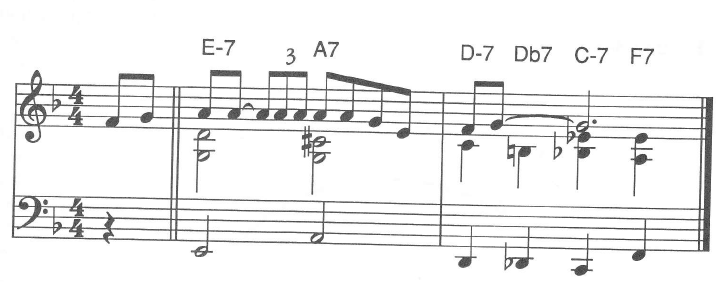
\includegraphics[width=5in]{levine_31.png}
\end{figure}

We first notice that most of the chords, as indicated by the associated chord labels, are incomplete; while the A7 chord contains root, third, fifth, and seventh, most of the other chords lack a fifth, and the ``D$\flat$7" chord also lacks a third.  If we are to apply Coker-style RNs, we will have to treat them as categories where entities like $(EGD)$ and $(EGBD)$ can both be called some kind of minor seventh chord.\footnote{Coker devotes little prose to voicing and omitted notes, but he does include a helpful Appendix B of suggested voicings; see pp.\ 83-84.}  The implied structures of the first two chords would then lead us to label them as II$^{m7}$ and V$^7$ in the key of DM.  The dominant chord should bring back the tonic chord, but what follows is a minor seventh chord (D-7) instead of a major or major-minor seventh.  For Coker, are these three chords a functional II-V-I progression?  The second bar contains two more minor seventh to dominant seventh progressions, the first of which does not reflect root motion on the circle of fifths.  Coker ultimately accounts for progressions like D$^{m7}$-D$\flat^7$-C$^{(M)7}$ by placing chords like $\flat$II$^7$ into the ``dominant" category on the basis of their intervallic structure and use, rather than their root motion.\footnote{See the table of equivalent functions given on p.\ 80.}  He does not, however, tell us whether we should call the D-7 in our example a tonic minor seventh (I$^{m7}$ in D), a subdominant minor seventh (II$^{m7}$ in C), or both.

%Levine
The example itself, the first two bars of Hill-Robinson's ``Old Folks," is annotated by Mark Levine and included in \emph{The Jazz Piano Book} (1989).  Like Coker 1964, Levine 1989 is a pedagogical treatise for the aspiring jazz player.  But instead of focusing on functional families of RNs, Levine identifies chords and progressions based solely on their most frequent usages.  This occasionally aligns him with Coker's subdominant-dominant-tonic (SDT) paradigm (as in his Chapter 2), but on other occasions it leads Levine to identify principles dictating chord progressions based on voicing or voice-leading concerns.  His Figure 3-1, reproduced as my Figure 1 above, is given an explanation of this type: while we might find II-V-I progressions in the passage, the more important observations, to Levine, are the root descents by fifth (except for the tritone substitution D$\flat^7$) and the consistent voice-leading pattern whereby the seventh of each chord descends by step to the third of the chord that follows.  The remainder of his work provides case studies of many chords and voicings which fall outside standard tertian labels and SDT harmony, and his approach is notable for its pluralism.\footnote{These case studies lead Levine to speculate about the best ways to label and explain such sonorities, and the results are sometimes thorny.  See \S 3 below for an illustrative example.}  While Levine's bag-of-tools approach provides helpful windows into particular forms of jazz harmonic practice, it does not provide a generalizable method for understanding the rules and conventions in play in many circumstances outside of his case studies, and it does not attempt to replace SDT syntax with any other conceptual framework.

Coker's conceptual simplicity and Levine's descriptive pluralism both fail to help us in the case of Figure 2, the opening 8 bars of Thelonious Monk's solo performance ``Memories of You."  For Coker to interpret RN functional progressions from the chord symbols supplied by the transcriber, he would first need to account for cases where the chord symbols themselves are wrong or misleading.  In m.\ 6, where is the $\flat$5 of the ``D$\flat 9\flat 5$" chord?  And what differentiates it from an inverted E$\flat^{7\flat 5}$ chord?  Even if the chord symbols all accurately represented Monk's musical surface, the unusual chord voicings and pitch structures would prevent us from assigning clear RNs or SDT functional labels.  Levine's attention to voicings might help us to identify a few more likely chord structures.  His observation in chapters 7 and 8 that dominant chords often replace a 5th with a 13th and employ a $\flat$9th might help us to contextualize the E13$\flat$9 of m.\ 5 as an altered dominant of the following Am chord;\footnote{See Levine 1989, pp.\ 41-58.} this functional association is strengthened by the circle-of-fifths root motion.  If one wanted to continue that reading, the ``D$\flat$9$\flat$5 C9" of m.\ 6 might be contested in favor of D9 (with no 3rd) preceded by a chromatic embellishing chord (E$\flat$7$\flat$5/D$\flat$). That would produce a descending 5ths sequence in mm.\ 5-8, starting on B and ending on F$^{M9}$ (the global tonic) in m.\ 9.   But such a reading does not demonstrate the necessity of a particular syntactic principle.  Rather, it \emph{assumes} syntactic principles and attempts to reduce the surface to those assumptions.
%FIGURE 2: Monk's ``Memories of You," the weird chord in m. 5
\begin{figure}
	\centering
	\caption{The opening 8 bars of Thelonious Monk's solo performance ``Memories of You."  Transcription taken from \emph{Thelonious Monk plays standards}.}
	\includegraphics[width=6.5in]{diss_prospectus_monk.png}
\end{figure}

%Russell
Of course, pedagogical manuals like Mehegan's, Coker's, and Levine's are only indirectly meant for analytical tasks, and their descriptions of harmonic progressions in jazz can train jazz musicians without providing a method for investigating cases like Monk's above.  Some pedagogical works even seem to directly contradict the inclinations of analysts while aiding the performer: George Russell's \emph{Lydian Concept of Tonal Organization} (1953) employs an infamously idiosyncratic RN notational system to lay out the basis for his highly influential chord-scale theory.  Russell provides instructions for determing the ``parent scale" of every chord.  This parent scale will allow the improviser to construct melodic lines which sound appropriate over the harmony under consideration.  Russell determines the parent scale for a chord by seeing which scales can accomodate the notes of the chord most readily.  He then assigns the chord a RN based on its intervallic distance from the ``lydian tonic" of that scale.

The melodic possibilities for improvisers are rich, but the implications for RN syntax are dire.  Both chords of an E$\flat ^7$-A$\flat^{M7}$ progression, for example, draw notes from the D$\flat$ Lydian parent scale.\footnote{For Russell's description of E$\flat^7$ and the D$\flat$ Lydian scale, see pp.\ 4-15.  Note that my hypothetical A$\flat^{M7}$ could also be based on the tonic of the A$\flat$ Lydian scale; Russell will later appeal to this fact and calculate chord-to-chord distances based the distance between the parent scales of chords, rather than the distance between the chords within a single Lydian parent scale.}  Based on the distances of the chord roots above the Lydian tonic (D$\flat$), Russell might initially seem to suggest RNs II$^{(7)}$ and V$^{(M7)}$ (in D$\flat$ Lydian) where most analysts would indicate V$^{(7)}$-I$^{(M7)}$ (in A$\flat$ Major).  Since A$\flat$ Major and D$\flat$ Lydian share the same diatonic collection, this amounts to a change of centricity, and the RNs correspondingly don't seem to align with their traditional uses.

To partially mitigate this, Russell postulates a separate ``over-all parent Lydian Chromatic Scale," in which he tracks chord-to-chord motions within a piece; the key of the piece is meant to correspond to the Lydian tonic of the over-all parent Lydian Chromatic Scale.\footnote{The Lydian Chromatic Scale is simply a somewhat-misleadingly named chromatic scale.  It receives its unusual moniker by subsuming the (variously altered) Lydian scales which share its Lydian tonic.  See Lesson II, pp.\ 9-15.}  Chord progressions are then captured in Russell's system by attending to the distances between the parent scales of each chord relative to the over-all parent Lydian Chromatic Scale.  This rather baroque method of chord relation only allows Russell to specify suggested chord relations as those whose parent scales bear ``close relationships."\footnote{See Lesson VIII, pp.\ 42ff.}  Since the Lydian scales with tonics separated by a fifth will only differ by one accidental, the resulting measure of closeness will be identical to the usual circle-of-fifths distance.\footnote{To put this another way, Russell's change of centricity from the Ionian to Lydian modes is independent of the voice-leading distance between diatonic collections.}  A descriptive syntax drawn from Russell's system will share closeness measures with more traditional RN users, but the ``rules and conventions" of the syntax will not align with classical conventions or help us to disambiguate difficult cases like Figure 2.

For each of the authors above, syntactic progressions in jazz seem to consist of root motions along the circle of fifths lensed through a series of additional constraints.  For Coker, differing chord qualities (minor seventh, dominant seventh, and so forth) give rise to SDT functional categories indexed by RNs.  Motion between categories often consists of root motion by fifths, but specific exceptions are made to accommodate cases where the chord \emph{functions} as an S, D, or T without matching the expected RN labels.  For Levine, circle of fifths root motion can be lensed through an idiosyncratic plurality of voicings and voice-leading techniques to produce differing progressions.  As I will show in \S 3 below, Levine readily relaxes root motion by fifth to describe harmonic patterns which seem to reflect some other kind of functional orientation, the identification of which usually depends on bass motion and voice leading.  Russell's motion by fifths is lensed through parent Lydian Chromatic scales, permitting wide improvisation but only imprecise notions of chord-to-chord syntax.  These models allow their audiences to generate convincing jazz, but they struggle to produce a generalizable description of harmonic syntax capable of parsing difficult or ambiguous pieces.  In search of analytical applications, we may turn to theoretical works less concerned with pedagogy.

\subsection{Theoretical/Analytical Approaches}
%Martin, Larson, Strunk?
Henry Martin's 1980 dissertation begins by stripping his description of harmonic progression in jazz all the way down to the circle of fifths.  Rather than modifying tonal models to account for unusual substitutions, Martin observes that the chromaticism of many jazz performances ``seems to suggest no prior diatonic model at any level."\footnote{Martin 1980, p.\ 7.}  With the possibility of many applied and altered dominant chords, substitutions involving chords taken from divergent diatonic collections, and chromatic root motions, jazz harmony may require descriptive tools from outside the tonal workshop.  To make matters more complicated, Martin notes that triads are often rare or nonexistent in jazz performances, replaced instead by extended chords which frequently omit fifths and ``are often not dissonant at any structural level."\footnote{Ibid.}  Tertian, tonal RN models are not guaranteed to get us very far.

After these caveats, Martin explains that partially-tertian extended chords, which he considers the norm in many jazz styles, can usually still be arranged in such a way that a root may be determined-- usually as the lowest pitch of a stack of thirds.  Moreover, the roots of these chords in jazz tend to progress by fifth or by semitone.  In claiming the functional equivalence of these root motions, Martin elevates the tritone substitution of $\flat$II$^7$ in place of V$^7$ to a general syntactic principle.  With this syntactic rule in play, Martin turns to a description of the voicings and voice-leadings most commonly employed for each extended chord type, separately describing the idiomatic ways in which seventh chords, ninth chords, eleventh chords, and so forth participate in syntactic root motions.  To analyze a particular harmonic progression, all the Martinian analyst needs to do is thus choose the degree to which extended chords are in play and look for the appropriate voice-leading patterns and root motions.  No RN background is required; the resulting harmonies are sufficiently constrained by the root motion and voice-leading paradigms.\footnote{In fact, Martin seems to think that the types of chord structures which appear over bass notes may be determined by the equivalence of fifth/semitone root motion and efficient voice leading.  ``For example," he says, ``the two possible roots line successions are by perfect fifth or semitone; the constructed harmonies must be compatible with either mode of succession" (p.\ 30).}

In later work, Martin explains that the circle of fifths ``is useful in understanding jazz harmony because it offers a simple picture of harmonic motion in instances where traditional roman numeral designations may be unnecessarily complicated or less apt."\footnote{Martin 1988, p.\ 12.}  Unfortunately, the circle of fifths itself proves insufficient to explain cases of differing chord quality or ambiguous roots.  I consider Martin's conscientious consideration of extended chord voicings admirable and worthy of emulation, but his reliance on the fifth/semitone circle leads to some handwaving over progressions that look like IV-V, and his tertian constructions are not readily generalizable to non-tertian sonorities.\footnote{See, for example, Martin 1988 p.\ 10, where he claims that IV chords are enough like II$^{m7}$ chords that they usually need not be considered separately.}  For Martin to connect these cases to his syntactic rules, he must provide derivations meant to reduce them to the simpler cases he considers.  To call a IV chord an incomplete II$^{m7}$ chord, Martin must hypothesize an absent root, and to account for quartal harmonies, he would need to rearrange the pitches in register and possibly remove some of them.  Both of these activities would bring the music within reach of his analytical system, but neither would demonstrate that the syntactic rules of his system operate in these contexts.\footnote{I will return to what I consider to be the perils of reduction immediately below and also at greater length in \S 4.}

%Larson (Strunk?)
Steve Larson attempts to systematize the process of removing difficult-to-explain notes by appealing to Schenkerian principles.  In his \emph{Analyzing Jazz -- A Schenkerian Approach} (2009), based on his dissertation research, Larson defends his extension of Schenker's tonal analysis techniques into jazz.  As part of the second chapter's methodological exploration, the consonant or dissonant status of extended harmonies appears to be a thorn in Larson's side.  Citing earlier Schenkerian work by Strunk (1985), Larson claims that many of the ninths, elevenths, and thirteenths of jazz are motivated by purely melodic concerns, rather than as part of chordal harmonies.  He acknowledges their frequent appearance in jazz while simultaneously downplaying their harmonic importance: ``Although these notes may receive greater emphasis and may be treated more freely in modern jazz than in classical music, their basic meaning remains the same: they derive their meaning from more-stable pitches at deeper structural levels."\footnote{Larson 2009, p.\ 6.}  Larson admits the existence of some ``polychords" and ``color" dissonances in the music of Monk, but by and large does not allow non-triadic tones to hold harmonic importance.\footnote{This stands in stark contrast to McGowan 2008, who claims that some non-triads (like the major seventh chord) are treated as fundamentally stable in jazz, requiring no dissonance resolution on any structural level.}

A more thorough critique of the syntactic implications of this view is included in \S 4 in the context of the Schenkerian techniques of Lerdahl and Jackendoff.  Here, it suffices to say that a reductive Schenkerian approach like Larson's does not seem capable of producing any harmonic syntax other than the assumed Schenkerian tonal harmony to which the jazz examples are reduced.  This is the easiest way in which we might interpret Mehegan's claim that the rules and conventions of jazz harmony are identical to those of western classical harmony-- if we ignore all the notes that cause the chords to differ from their earlier counterparts, it is possible to shoehorn the rest into extant tonal theory.  This does not seem productive, to me, as it leads us to reduce away exactly those notes which seem to make jazz harmony so interesting.  In providing a series of Schenkerian reductions away from these harmonies, Larson can demonstrate that it is possible to fit the jazz surface to a classical background with an appropriate system of erasures replacing ``dissonant" tones with their ``more stable" neighbors, but he cannot show that the harmonic progressions of jazz are best described in this way or account for the particular deployments of extended voicings.  Put more provocatively, we cannot expect to find new syntactic principles by reducing away anything which does not conform to the old ones.

\section{Components of Harmonic Theory: Labels and Syntax}
Instead of assuming a tonal syntactic background and reducing jazz harmonic surfaces to it, my project aims to demonstrate syntactic behavior drawn from the surfaces themselves.  Like the work of the theorists above, I intend to construct categories of chord function, but they will not be defined \emph{a priori} by chord quality or RN label; instead, I will separate the labeling of jazz harmonies from syntactic assumptions and look for patterns of harmonic progression in a large corpus of jazz solos.  By examining chord-to-chord motions without reference to a tonal center, diatonic collection, or tertian chord construction, I will provide a method for investigating the functional behavior of any common type of chord structure employed in a jazz style.\footnote{While the corpus I am envisioning should be easily customizable, including the capability to restrict results to certain artists or communities, the exact styles represented will depend on my ability to obtain and encode transcriptions.}  Like Levine, I will describe non-tertian sonorities based on their functional deployment in progressions, but my results will be based on corpus data and will demonstrate a consistent and syntax-free chord labeling system.  Like Martin, I will take extended chords seriously, looking for the most common chord-to-chord voice leading patterns for each type of chord configuration.  And as Mehegan's claim (2) implies, I will produce a theory of jazz figured bass, though its labeling and syntactic categories will differ completely from Mehegan's.  A more complete statement of my project appears in \S 5.  Before presenting it, I will tackle the two components of my methodology separately.

\S 3 begins by interrogating Mehegan's claim (2).  I will discuss chord labeling techniques employed by theorists like Mehegan and Levine in an attempt to show that the choice of label for many jazz chords is not unique.  In the case of RN labeling, deciding on one label over another seems to be primarily based on syntactic intuition.  Since the resulting labels depended on an assumed syntax for their production, they cannot be used as evidence for the syntax itself without begging the question of where the syntax came from in the first place.  This section will motivate the syntax-free labeling I introduce in \S 5.

\S 4 will turn to the concept of syntax itself.  If, as I claimed in \S 1 above, the background ``rules and conventions" of classical and jazz harmony (to which Mehegan's claim (1) refers without explicit reference to syntax) have often been implicitly considered a form of syntax, the roots of this usage lie in \emph{linguistic} theories of syntax and their importation into music theory in the latter half of the twentieth century. The influence of Chomskyian generative grammars will help us make sense of how theorists conceptualize ``rules" of syntax which do not immediately appear on musical surfaces.  I will connect the deep and surface structures of Chomskyan generative grammars to theories based on Schenkerian principles and question whether such theories can demonstrate harmonic syntax.  Questioning the importation of Chomsky's structural levels into music in general, I will advocate replacing generative, deep-structural tools with Markovian, surface-structural ones, particularly in computational corpus-analysis settings.

In \S 5, I then aim to propose a corpus analysis project which draws on non-generative theories of syntactic structure to produce a syntax-free labeling system for chords and a functional description of harmonic succession in jazz free of the epistemological pitfalls of either generative linguistics or roman numeral analysis.  My modern-day jazz ``figured bass" will hopefully allow me to assemble categories of functional chord motion based solely on the musical data at hand.  The resulting harmonic syntax will reflect the properties of the jazz corpus employed, rather than the preconceptions of any particular tonal labeling system.

\section{Chord Labeling}
I consider the process of labeling Mehegan employs to be a case study which reveals the difficulties of determining chord identity.  Mehegan's claim (2) proposes a jazz ``figured bass," but his subsequent presentation only partially conforms to the figured bass tradition.  To build his figured bass, Mehegan immediately (and somewhat unexpectedly) imports roman numeral (RN) analysis from the western music theory tradition, conflating two strains of thought with different histories and grounding assumptions.  Notably, the 17th and 18th century figured bass tradition to which Mehegan presumably refers did not employ or require roman numeral labels of any sort.\footnote{For typical eighteenth century examples of the figured bass tradition to which I refer, see Heinichen 1711 and 1728 and Mattheson 1739.  By the mid-eighteenth century, thorough-bass manuals imply recognition of fundamental bass principles, and notational systems begin to make systematic use of RNs with Vogler 1776.  While figured bass and fundamental bass are brought into contact via RNs in this and later works, RNs themselves do not constitute a formative or crucial part of the figured bass tradition.}  Mehegan's reason for employing them in the context of figured bass is primarily one of convenience, as he claims that ``with figured bass one spelling using numbers can be used for twelve keys, since the relationships in one key obtain  for all other keys."\footnote{Mehegan 1959, p.\ 8.}  Instead of specifying a literal bass line (as in 17th/18th-century figured bass practice), Mehegan opts to employ a roman numeral stand in.  This provides musicians a way to memorize chord relationships without making reference to any particular key, which allows for easy transposition when working with a shifting ensemble of players with different backgrounds and preferences.  Mehegan criticizes lead sheet notation, which, as he points out, does not provide this transpositional convenience.\footnote{By ``lead sheet notation," Mehegan means harmonic short hand like ``A$^{\flat 7 \sharp 11}$," which would later be epitomized by the underground ``Real Book" circulations begun at Berklee and adopted and licensed by Hal Leonard in 2004.}  This appears to be the most common justification given in the jazz literature for the use of RNs, and it appears to be the primary motivation behind Mehegan's figured bass.

%Assumptions of Mehegan's RNs (at least initially)
When treating root position diatonic seventh chords relative to a common global key center, RNs can unambiguously indicate figured bass.  To generate a suitable label, all the player needs is to look at the bass note of the chord, calculate its (diatonic) distance from the key center, write a roman numeral to represent this distance (``Distance can best be described by number"\footnote{Mehegan 1959, p.\ 8.}), and then indicate with figures what notes appear above this bass note.  This is an appropriate and useful application of figured bass, and it relies on several assumptions.  When Mehegan applies RN $\alpha$ to a chord $X = (x_1,x_2,x_3,x_4)$, he implicitly claims the following:\
\begin{enumerate}
	\item There exists a tonic note $y_1$ such that we may construct a chord $Y = (y_1,y_2,y_3,y_4)$ and label it I
	\item The note $y_1$ is the tonic note of a diatonic collection, and the bass note $x_1$ of chord $X$ lies $\alpha -$ I diatonic steps above $y_1$
	\item The upper voices of chord $X$ may be derived from the diatonic scale of $y_1$; this is done by stacking three diatonic thirds above the bass note $x_1$, unless otherwise specified.  (This produces, in Mehegan's terms, ``scale-tone seventh chords."\footnote{Ibid., p.\ 11.})
\end{enumerate}
In other words, the importation of RNs brings with it assumptions of key centricity,\footnote{I will define this below, but note that I do not mean key \emph{specificity}-- RNs assume no key in particular, but they do assume that there is one key center. Mehegan does not provide much guidance as to how we might determine the key center of a passage.  In most of his examples, he presumes the key is obvious.  This, alongside his aversion to minor keys, leads to some odd analyses: lesson 22, for example, describes an unproblematic d-minor tune with RNs taken exclusively from FM, yielding many odd IIIx - VI$^{+6}$ progressions.} diatonic collection, and chord construction.  Before we examine Mehegan's subsequent use of RNs, I might pause here to describe these three assumptions in terms similar to those used by Dmitri Tymoczko in \emph{A Geometry of Music}.  In chapter 1, Tymoczko conjectures that most music we would call ``tonal" bears five important features: conjunct melodic motion, acoustic consonance, harmonic consistency, limited macroharmony, and centricity.\footnote{See Tymoczko 2011, chapter 1, especially pp.\ 3-7.}  Of these, the assumptions I listed above most immediately involve the last three.

%Description of centricity, diatonicity, and chord construction, bringing in Dmitri
Assumption (1) maps directly onto Tymoczko's description of centricity.  In general, the tonal center $y_1$ can be asserted with or without a coherent diatonic setting; in some circumstances, the identification of a tonal center may boil down to a simple statistical claim.  If pitch $y_1$ appears more frequently than any other pitch, we might be inclined to recognize it as a tonal center.  Many other criteria might be brought to bear on this determination: the harmonies deployed, metric structure, melodic shaping, dynamic or agogic accents, texture and instrumentation, or formal structure might all contribute to (or problematize) the identification of a tonal center.  In principle, however, no one of these indicators in particular is required.  In analogy with geometry, the tonal center is merely a choice of the origin point for our coordinate system; we will reckon the distances of other notes based on $y_1$, and we need not make any particular assumptions regarding diatonicity, function, or syntax to do so.

%Monk example of the difficulty of stack-of-thirds labeling
Assumption (3) links the centered, diatonic collection to the construction of the chord $X$.  Given a RN $\alpha$, we may construct a chord in Mehegan's system by moving $\alpha$ diatonic steps above the tonic and then stacking three diatonic thirds.  Conversely, when we see a stack of diatonic thirds, Mehegan instructs us (in the simplest case) to identify the diatonic scale from which the chord tones are drawn and apply a RN label accordingly.  This assumption, taken at face value, restricts the domain to which RNs may be applied in jazz; the chord construction of non-tertian voicings may fail to provide an adequate basis for Mehegan's RNs.  For an example, we can return to the opening run through the changes of Thelonious Monk's solo performance ``Memories of You" (Figure 2 above).  The transcription I have excerpted provides a quixotic lead sheet symbol for the chord on the downbeat of measure 5.  Examining the chord in isolation, we immediately realize we cannot directly satisfy assumption (3), since the pitch classes present cannot be generated by stacking diatonic thirds atop the bass -- in fact, we cannot even rearrange the voices to see a well-formed seventh chord built by stacking thirds on any note of the chord.
%FIGURE 1: Monk's ``Memories of You," the weird chord in m. 5
%\begin{figure}
%	\centering
%	\caption{The opening 8 bars of Thelonious Monk's solo performance ``Memories of You."  What chord falls on the downbeat of measure 5?}
%	\includegraphics[width=6.5in]{diss_prospectus_monk.png}
%\end{figure}

Stepping outside of the literal instructions I have so far attributed to Mehegan,\footnote{Mehegan himself soon steps outside this procedure, to his credit; see below.} the closest we might get would be to rearrange the chord as $(G, B\natural, F, A)$ and parse it as some kind of inverted G chord missing a fifth and with an added ninth.  The lead sheet, however, considers the chord a ``Bm7$\flat$5(add$\flat$6);" while this notation does not reflect the fact that the ``Bm7" lacks a third, it does capture the contextual root motion as part of an embellished sequence of descending fifths.\footnote{This reading runs into the same problems identified in \S 1.1 above, especially regarding the interpretation of the ``D$\flat$9$\flat$5 C9" chord.}  This kind of contextual analysis, however, appeals to an observed pattern of \emph{use}, rather than the literal construction of the pitch class set, to help apply a label to the chord.  I will return to this as a grounding for the notion of ``function" over the course of my dissertation, but for now it suffices to notice that this parsing is well beyond the instructions provided (or even permitted) by Mehegan's system, formally speaking.

This is not to say that application of RNs will be impossible in such cases, but rather that the application of \emph{these particular} RNs will be impossible.  Unless a passage displays centricity, diatonicity, and tertian chord construction, Mehegan's RNs do not necessarily apply.  Many scholars will relax one or more of Mehegan's three assumptions above in order to reconfigure RNs in the context of a new or less frequently explored repertoire, performing this conceptual shift explicitly or enacting it behind the scenes.

The news that quite differently-defined entities may masquerade (or brilliantly function) under the name ``roman numeral" will come as no surprise to those familiar with the jazz theory literature.  In fact, RNs often appear in implicitly or explicitly different formulations within a single work by a particular scholar.  To assess the syntactic claims of jazz theorists regarding the deployment of chords labeled by RNs, we must first understand what these RNs specify and how they are produced, lest we misinterpret them as syntax-free labels we can use as evidence for our harmonic theories.  One of my purposes here, then, is to examine the definitions and uses of RNs in the work of several prominent jazz theorists.  I will allow this collection of writings to guide me in mapping out what parts of the jazz repertoire may benefit from the application of RNs.  As I attempt to describe these theorists and their work in terms of the assumptions of centricity, diatonicity, and chord construction, I hope to suggest an alternative, more flexible formulation-- one which might remove tonal assumptions from the labeling.

\subsection{In Search of Roman Numerals}
%Review of jazz theorists (and their associated repertoires) to see how these assumptions play into their use of RNs.  Mention that Mehegan starts to get confusing when he switches to fundamental bass (inverted chords).  Start with Mehegan as he confuses his concept of figured bass, changing his definitions for RNs.
Mehegan steps away from the RN definition set out in his introduction and first three ``lessons" almost immediately.  After constructing the diatonic (``scale-tone") seventh chords by following the procedure outlined above, he shows how five qualities of seventh chord are produced in this manner (major, dominant, minor, half-diminished, and diminished); due to the coordination of diatonicity and centricity, each RN necessarily results in one particular quality of seventh chord.  ``In other words," Mehegan writes, ``The I chord is always \textsc{major}, the II chord is always \textsc{minor}, the III chord..." \footnote{Mehegan 1959, p.\ 19.}  Again: given a key center and a diatonic collection, each RN uniquely defines a particular chord.

In lesson 4, Mehegan introduces commonly ``altered" notes into his scale-tone seventh chords.  ``Jazz harmony is extremely chromatic," he writes, ``and it is important to be able to build any quality at any point in the scale."\footnote{Ibid., p.\ 21.}  A RN no longer requires one and only one chord; now, the RN label may include a list of symbols indicating which quality alterations are present (in his system, these include symbols like x, m, $\phi$, and o).  This addition widens the applicability of Mehegan's RNs while retaining his figured-bass orientation; the RNs themselves function as (particular) key-free stand-ins for bass notes, and the alteration letters function as symbolic figured bass numbers.  Chords are still stacks of thirds built on scale tone bass notes some number of diatonic steps away from a tonal center.  The stacks of thirds themselves, however, are no longer necessarily drawn from the same diatonic scale as the key center or the chordal bass-- or indeed from any diatonic collection, as seen in the chord $(C,E\flat,G\flat,A)$, which Mehegan labels ``Io" in CM.\footnote{Vol.\ 1, p.\ 22.}

%Unpack ``traditonal RN theorists" more? I use A&S to distinguish between RNs and figured bass, but I could go back to more historical sources.
In lessons 5-7, Mehegan finally relaxes the condition of diatonicity completely, instructing the reader how to build seventh chords of any quality over a bass note any distance from the key center (such as $\sharp I$, $\flat VI$, and so forth), and the condition of tertian chord construction partially, demonstrating how stack-of-thirds chords can have non-thirds added to them (especially sixths above the bass).  At this point, Mehegan has a fully functional figured bass notational system requiring only key center and partly-tertian chord construction; the initial diatonicity is no longer necessary.  Identifying literal bass notes instead of roots, his RNs notate a kind of thoroughbass, rather than a fundamental bass, and they leave open the possibility of added non-tertian upper voices.  I note that, as such, his RNs do not yet behave in the way that traditional RNs (i.e., those from the classical tradition) do.  Consider the contrasting case of the standard textbook picture of root-centric inversional categorization provided by textbooks like Aldwell and Schachter, in which ``the roots can by indicated by roman numerals, and the inversions, if any, by figured-bass symbols."\footnote{Aldwell \& Schachter 2003, p.\ 55.}  Drawing on the tradition of Weber and Vogler, Aldwell and Schachter explain that ``Roman numerals and figured-bass symbols show very different things.  Roman numerals indicate the \emph{roots} of the chords and the scale degrees on which they fall.  Figured-bass symbols are calculated from the \emph{bass tones}, not the roots, so that we do not need to think of the chord roots to realize a figured bass."\footnote{Ibid.}  For the first 20 lessons of Mehegan's work, this distinction is ignored.

My rather pedantic summary of these opening lessons is to this end: lesson 21 lays bare a conflict between figured bass and traditional roman numeral theory.  Entitled ``Inversions," lesson 21 suddenly identifies chords by their roots rather than by their bass notes, though Mehegan does not describe the notational shift in these (or any) terms.  Now the labeling system faces a serious ambiguity which surfaces in a large number of jazz theories (and some classical ones).  To put it in a simple form: what is the RN label for the chord in Figure 3?
%FIGURE 3: (CEGA) CHORD
\begin{figure}
	\centering
	\caption{Is this common chord a triad in root position with an added sixth, or a seventh chord in first inversion?  On what grounds should we make this decision?  Does the distinction matter for assembling a theory of syntax?}
	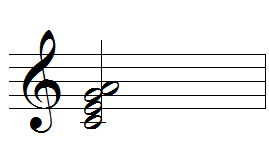
\includegraphics[width=1.6in]{diss_prospectus_cega.png}
\end{figure}

Up through section 20, Mehegan has labeled such chords (in the key of CM) as I$^{+6}$.  Beginning in section 21, we should be inclined to apply the label VI$^6_5$.  Even assuming a stable and unambiguous key center (here, CM), the literal notes of the chord no longer suffice to determine its proper label; the exact same chord in Figure 3 receives the label ``I+6" on p.\ 30, while it is parsed as ``Am$^6_5$" on p.\ 45 (corresponding to VI$^6_5$ in our hypothetically-unambiguous CM key).  Chord identity is now fundamentally fuzzy,\footnote{I mean ``fuzzy" in the mathematical, set-theoretic sense; some II chords may now seem ``more-II-like" than others.  This concept is fruitfully imported into the music theory literature by papers like Quinn 1997 and 2001.} as non-tertian pitch structures may be identified as root-position triads with added notes (in figured-bass terms) or as inverted triads with or without added notes (in fundamental-bass terms).

%Bring in discussion of function here?
In the case of Figure 3, the labeling distinction seems to have little impact on a resulting theory of syntax.  In the western classical syntax assumed by Mehegan, both VI and I$^{+6}$ (to keep Mehegan's terms) have a kind of ``tonic function" in the music of Chopin and other romantic composers, if we partake of the functional harmonic tradition traceable back to Riemann.\footnote{Tonic, subdominant, and dominant functions are first systematically laid out in Riemann's \emph{Vereinfachte Harmonielehre oder die Lehre von der tonalen Funktionen der Akkorde} of 1893.}  In Riemann's usage, the two chords are similar in that they are closely related: one is the relative minor (or major) of the other.  This claim of similarity does not require an examination of the actual successive deployment of these chords (i.e., their behavior in chord progressions), but rather a process for reducing one to the other used to construct a kind of structural equivalence class.  To Riemann, this similarity gives rise to the fact that I and VI are used in similar progressions-- and it is to this shared pattern of use that scholars usually refer when they discuss ``functional" harmony.\footnote{See, for example, Tymoczko 2011 \S 6.4 (pp.\ 212-214) and Chapter 7 (pp.\ 226ff).}  

Mehegan seems to use an adjusted and more specific notion of function, claiming that ``I$^{+6}$ is also VI$^{6}_5$, but the function of the chord is usually an adjusted I chord rather than an inverted VI chord."\footnote{Mehegan 1959, p.\ 47.}  This ``tonic function" has no necessary connection to the labeling procedure he employs, and it is evidently tied to the behavior of the chords in harmonic progressions-- their syntax.  To borrow terms from the linguistics I will discuss below (in \S 4), users of Riemannian function and Mehegan's function both construct syntactic categories, ``phrase constituents" of sorts which characterize the categories' members by the well-formed progressions in which they are involved.  In saying that the function of an ``adjusted I chord" differs from that of ``an inverted VI chord," Mehegan seems to make a subtle distinction between two different musical parts of speech.  The rules of a harmonic syntax should teach us how to order the things we identify as phrase constituents; if those things are categories of chord function, then we need a lexical classification scheme (telling us which kinds of chord fall into each category) and a set of syntactic progression rules (telling us which progressions are well-formed).

In this case, the lexical categories into which the ambiguous chord could be placed are likely to behave similarly with regard to the rules of the syntax.  This means that our labeling decision has a relatively small impact on what kind of syntax we are likely to describe for a passage (or style) in which the chord of Figure 3 features.  And aside from function, we might expect to use the assumptions of centricity and chord construction to help break the label degeneracy.  If the key center is $CM$, chords built on scale degree $\hat{1}$ are probably (though not necessarily) more frequent than chords built on scale degree $\hat{6}$, and if the most common chord construction involves placing the root in the bass, we ought to be willing to label the chord I$^{+6}$.  This might get us out of trouble in comparatively simple cases.\footnote{Note that the problem multiplies as even diatonic cases become more ambiguous.  An analogous appeal to centricity and root-position chord construction might lead us to label $CM: (F,A,C,D)$ as IV$^{+6}$ instead of II$^{6}_5$, though this might suggest that we acknowledge a much wider application of IV \emph{vis-a-vis} II than is commonly accepted in the literature. And what about the chord $(E,G,A,C)$?  Even if we are certain that the key is CM, is this some kind of inverted I$^{+6}$ (for which our symbols would fail us-- perhaps I$^{+6,6}$ or I$^{6,+4}$), or a VI$^{4}_3$?  Or, less probably, if we take Mehegan's supposed figured bass very literally, is this some kind of III$^{\sharp 5, +4}$?}  Consider, however, the more difficult case given in Figure 4, where centricity and chord construction are unlikely to help us and the consequences of our labeling are significantly greater for our resulting syntactic description.
%FIGURE 4: SOME COMPLICATED NON-TERTIAN CHORD THAT MIGHT BE AN INVERTED CHORD
\begin{figure}
	\centering
	\caption{An ``E Phrygian" chord, used in Mark Levine's introduction to Sus and Phrygian chords.}
	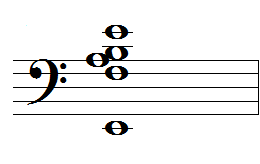
\includegraphics[width=1.6in]{diss_prospectus_ephryg.png}
\end{figure}
%Footnote it someplace: \footnote{Levine 1989, p.\ 25.}

In cases like these, the application of RNs can result in many different labels, depending on which assumptions and procedures we preference.  The chord does not immediately appear tertian in construction; no amount of inversion will allow us to rearrange this verticality as a stack of thirds.  The general reaction to non-obviously tertian or diatonic chords in jazz seems to consist in producing a story of its generation in which the ``unusual" sonority is neutralized by its reduction to more ``normal" chords, a sort of modern-day replication of Riemann's tendency to reduce chromatic chords to expected functions.  Mehegan's text does not provide one for the chord of Figure 4, which rose to prominence only in the 1960s, so we might return to the later work of Mark Levine for help.

\subsection{Use vs.\ Pitch-class content}
Levine employs primarily lead sheet notation for his examples, eschewing RNs whenever possible.  To make sense of the chord in Figure 4, Levine starts by notating a ``G7" chord.\footnote{Levine 1989, p.\ 25.  It is worth noting that his G7 chord contains the registrally-ordered pitches (GFABE); the re-ordered stack of thirds would be (GB-FA-E), where I have placed hyphens in the place of omitted notes.  ``G7" thus stands as a rather incomplete (or at least classically atypical) description of the chord, which contains no fifth and an added ninth and thirteenth.}  Levine considers this to be a dominant seventh chord, thanks to its structural major third and minor seventh above the root.  Inverting the G7 to place the E in the bass, according to Levine, changes the function of the chord: ``Even though G7 is a V chord in the key of C, the V-I relationship here is between E and A."\footnote{Ibid.}  Here, we see one of Levine's rare appeals to RNs.  Evidently, while the \emph{configuration} of this chord (that is, the pitch and interval content) does not indicate its syntactic role as V in A (it is missing a third, fifth, and seventh), its \emph{function} is nevertheless a dominant one in this key, and Levine likens it to a classical ``Phrygian" cadence.\footnote{This dominant flavor might come from the $\flat$9 above the bass; Levine constructs dominant sevenths with this interval in chapter 8 (see p.\ 49).}  When Levine uses the term ``V," he establishes a lexical category quite different from the vertical structure-oriented categories seen in Mehegan's work: here, the pitch class set entirely matches that of a G7 (up to Levine's voicing options, not rehearsed here), but the ordering and deployment of the set instead places it into the category of a V chord in A-- despite its missing third and seventh, two notes considered important to a chord's functional identity.  We seem to be forced to label the chord either by its pitch content or by its use, and the resulting application of RNs is left ungrounded.  ``V" may no longer resemble a diatonic, tertian seventh chord, but rather a lexical category of morphologically dissimilar entities which function in similar ways.

In the context of a passage in AM, the choice of label for this chord provides ideas of syntax which differ more than in the case of Figure 2 above.  If we choose to label it as an inversion of G7, our syntactical parsing will reflect a RN motion $\flat$VII-I; if we choose E Phrygian, the ``root" motion between two chords will instead lead us to describe the harmonic progression as some kind of V-I motion.  The resulting theory of syntax will be guilty of question-begging; in assembling the labels off of which the syntactic observations will be based, we must invoke the contextual syntax itself to override or augment a pitch class set-based lexical classification scheme.

In order to explain away the pitch class content of chords like this when placing them in a structurally-unexpected lexical category (like one based on the V function), analysts employ a variety of reductive techniques designed to account for the disparity between a chord's contents and its use-based label.  Syntactic demonstrations drawing on methods like those of Mehegan and Levine would then trace the following path:
\begin{enumerate}
	\item Begin a description of jazz syntax by categorizing chord-to-chord successions.
	\item Establish figured bass-oriented labels based on centricity, diatonicity, and tertian chord construction (though the latter two of these assumptions can be relaxed); implicitly identify fundamental bass (via root tones) with figured bass (via bass tones).
	\item Notice that non-tertian and/or non-diatonic pitch stacks lead to fundamental bass ambiguity; figured bass and structural descriptions no longer capture intuitive sense of use (or lexical categories representing function).
	\item Abandon figured bass labeling in an attempt to indicate function; create generation/reduction procedures relating non-tertian/non-diatonic pitch stacks to centered, diatonic, tertian chords.
	\item Demonstrate syntactic function from the resulting labels-- though our assumptions about the expected nature of such syntax strongly informed our application of these labels in the first place.
\end{enumerate}

At stake here is not merely what notation we use to describe the E Phrygian chord.  Any syntax which purports to describe well-formed sequences of RN lexical categories based on centricity, diatonicity, and tertian construction will stumble with chords whose functional use seems to defy those structural categories, whether due to voicings, alterations, or some contextual phenomena.  It seems that the search for RN-based syntax requires syntactic assumptions for the generation of RNs.  If we wish to test a jazz repertory for syntactic progressions, we will need to first identify lexical categories in some more neutral way.

\section{Syntax in Music}% Syntax(es) and Musical ``Depth"}

In claiming identical ``rules and conventions" for jazz harmony and classical harmony, Mehegan's claim (1) subsumes several separate statements about conventional similarity.  First, it implies that the individual genres of Bach fugues, Mozart sonatas, and Brahms rhapsodies each have relatively homogeneous ``rules and conventions."  Second, it implies that these three sets of conventions are instantiations of an overarching set of rules called ``classical harmony;" while Brahms sounds like Brahms and Bach like Bach, there is some shared backdrop of harmonic processes at play in the works of classical composers.  Third, it implies that jazz music partakes of a homogeneous set of rules and conventions called ``jazz harmony."  Lastly, statement (1) above explicitly claims that the set of rules of this general jazz harmony are identical to the set of rules for general classical harmony.

I am deliberately (and somewhat unjustly) interpreting Mehegan's claim literally in order to indicate the complicated and potentially-contradictory conditions a harmonic theory must meet in jazz or any other music.  Mehegan does not pursue a monolithic and faceless jazz harmony; rather, in the remaining volumes of his work, he describes the practices of several prominent jazz pianists\footnote{In Vol.\ 3 consists entirely of individual studies devoted to Teddy Wilson, Art Tatum, Bud Powell, George Shearing, and Horace Silver, and Vol.\ 4 foregrounds the work of Oscar Peterson and Bill Evans.} in order to articulate a network of harmonic conventions, some of which are shared between many groups of performers (such as the A and B voicings of Vol.\ 4), and some of which are more typical of one practitioner or form of jazz practice than of others.\footnote{Some of the individualized tendencies Mehegan identifies relate to patters of alteration.  For example, Mehegan claims that some of Bud Powell's ``persistent idioms" consist of deploying raised 4th and 7th degrees and both raised and lowered 2nds above the root over ``Dominant Chords" (Vol.\ 3, p.\ 120).  Mehegan thinks that the structure of a dominant seventh chord exists behind (in some conceptual sense) the chords deployed by Powell and others, but that the notes which appear in the actual voicing of the chord and the resulting melodic lines are more a matter of individual preference.}  Mehegan clearly thinks that a relatively coherent set of harmonic ``rules" regarding chord structure and succession sits in the shared background of these forms of practice, but he also seeks to articulate differing interpretations of these rules.  Just as ``common practice tonality" provides a set of guidelines within which Bach fugues, Mozart sonatas, and Brahms rhapsodies participate with different conventions and practices, a successful theory of jazz harmony must describe a shared set of jazz harmonic rules, if one exists, and also allow us to describe the practices of particular jazz ``communities," be they geographical, temporal, or abstractly metaphorical.

To borrow a concept taken from Richard Wollheim and developed Whitney Davis, I might describe Mehegan (and Coker, among others) as a type of \emph{latent formalist}.  Latent formalists seek to describe a form of artistic practice by appealing to a language-like system underlying the surface organization and configuration of works.  A latent formalist description of a work then appeals to a set of syntactic rules which make the surface intelligible.  Mehegan thinks that each jazz musician he seeks to describe has a distinctive harmonic style composed of elemental techniques rendering it sensible and recognizable, a ``rule-book" providing ``a general method of [musical] composition."\footnote{Davis 2011, p.\ 59; I have replaced Davis's term ``pictorial" with ``musical," which I do not think changes the spirit of his remarks.}  ``Latent Formalism," as Davis describes it, ``claims to reconstruct the system behind such methods, the recipes and rules."\footnote{Ibid.}  Like Davis's latent formalists, the task of many jazz theorists seems to be to replicate the methods of jazz pianists by providing syntactic rules distilled from observation of the works themselves.

What is the nature of these harmonic rules and conventions?  The history of writing about music is littered with both typological and contextual laws meant to indicate which sonorities are appropriate or pleasing and when they might be deployed.  In the typological genre, I count traditional dicta regarding consonance and dissonance\footnote{For a good overview of these kinds of claims from a jazz perspective, see McGowan 2008.  We might also call arguments over whether a sound is musical or not (say, a lawn mower) similar in structure.} and restrictions on what kind of verticality is or is not permitted in ``musical" utterances generally-- rules of the form ``tritones, bird song, and car horns are not permitted in civilized music, while major and minor triads are."  Mehegan makes a claim of this nature when he asserts that ``Chords of less than a seventh are insufficient for jazz."\footnote{Vol.\ 1, p.\ 11.}

On the contextual side, I refer to descriptions of permissible sequences of verticalities-- rules of the form ``vertical array X may [not] follow vertical array Y."  Appealing to the circle of fifths, Mehegan offers contextual rules like ``III normally moves to VI."\footnote{Vol.\ 1, p.\ 158.  In \S 3, I will unpack the assumptions behind Mehegan's RN notation; for now, we may assume that III and VI refer to seventh chords built on the third and sixth scale degrees within a stable key.}  Whether based on supposedly natural laws, spiritual guidance, or examination of a specific repertoire, these ``laws" aim to articulate a set of constraints within which harmonies and their juxtapositions are recognized as appropriate and musical.  To phrase this in a more provocative way: these laws outline criteria for the well-formedness of harmonic successions.  They might be seen to form the basis for treating ``a work of art as if it had a linguistic identity or at least a language-like identity" -- the harmonic forms deployed by musicians are then ``constituted within the system in the same way as a well-formed sentence might be spoken by someone who knows the grammar of a language."\footnote{Davis 2011, p.\ 58.}  As a latent formalist like Mehegan considers the well-formedness of harmonic successions, he analogizes the process of constructing a solo to that of constructing a linguistic utterance.

\subsection{Well-Formed Language and Linguistic Components}

To describe the search for harmonic rules as the establishment of criteria for well-formedness is to partake of a twentieth-century music theoretical tradition whereby terminology and methods are imported from linguistics (and through linguistics, mathematics and formal logic); in music, as in so many other fields of the humanities, this means almost exclusively to borrow from the fertile and divisive ideas of Noam Chomsky.  Chomsky's \emph{Syntactic Structures} (1957) and \emph{Aspects of the Theory of Syntax} (1965) lay the groundwork for a structural and quasi-cognitive model explaining (or at least describing) the distinction between well-formed and malformed utterances in spoken or written language.  In these early works, Chomsky partitions linguistic performance into three interlocking components: the phonological, the semantic, and the syntactic, the last of which is of primary interest to him.\footnote{Chomsky 1965, p.\ 16.}  In language parallel to that of Mehegan, Chomsky defines syntax in passing:

``[This study] will be concerned with the syntactic component of a generative grammar, that is, with the rules that specify the well-formed strings of minimal syntactically functioning units (\emph{formatives}) and assign structural information of various kinds both to these strings and to strings that deviate from well-formedness in certain respects."\footnote{Ibid., p.\ 3.}

This ``definition" itself includes the term syntactic, so I might rephrase it in simpler language to remove some of the ambiguity: the syntactic component contains the rules that specify the well-formed ordering of whatever objects for which ordering carries structural importance.  For the syntax Chomsky describes, formatives are words composed of phonemes, and sentences constitute well-formed strings of these formatives.  The rules to which Chomsky refers and the ``structural information of various kinds" are not contained in the sentences of the language explicitly; rather, the grammar hypothesizes them and judges their accuracy and usefulness by its resulting ability to generate all and only well-formed strings.

As I see it, the structure of this syntax is informed by two key observations.  First, some English sentences can be grammatical without being sensible; the well-worn example is Chomsky's novel sentence ``Colorless green ideas sleep furiously."\footnote{Chomsky 1957, p.\ 15.}  For Chomsky, this sentence can be parsed syntactically with little problem; the subject is a noun phrase in which colorless and green are adjectives modifying ideas, and the adverb furiously modifies the action of ideas (sleep).  Semantically, however, this sentence fails to satisfy a literally-minded listener.\footnote{Though other scholars and artists have offered abstract or metaphorical interpretations of the sentence in an effort to render it ``sensible."}  This type of semantically-malformed sentence differs from syntactically-malformed sentences like ``Furiously sleep ideas green colorless"\footnote{Chomsky 1957, p.\ 15.} or ``sincerity frighten may boy the."\footnote{Chomsky 1965, p.\ 76.}  If sentences may be syntactically acceptable without being semantically parseable, the two linguistic components must be separable, at least to some degree.  Accounting for this phenomenon leads Chomsky to posit a deep syntactic background independent of and as input to semantic processing.

Chomsky's second guiding insight is the recognition that many apparently different sentences can be well-formed and convey the same semantic content.  That is, the differing ``surface structures" and phonological interpretations of sentences like ``I expected a specialist to examine John" and ``I expected John to be examined by a specialist" nevertheless correspond to identical deep structures upon which their semantic equivalence seems to be based.\footnote{Chomsky 1965, p.\ 22.}  Chomsky's syntax must now perform a difficult double duty: it must determine the phonetic interpretation (the sounding order and cadence of phonemes) as well as the semantic interpretation (some information regarding a referential claim to ``meaning") while preserving the possibility of similarity in one domain alongside difference in the other.  ``Consequently," he writes, ``the syntactic component of a grammar must specify, for each sentence, a \emph{deep structure} that determines its semantic interpretation and a \emph{surface structure} that determines its phonetic interpretation.  The first of these is interpreted by the semantic component; the second, by the phonological component."\footnote{Chomsky 1965, p.\ 16.}  Having isolated the syntactic component of linguistic ability, Chomsky partitions it into distinct levels, one of which must necessarily stand as an abstraction from the observed ``surface."

At this point, it might be productive to take a brief aside in the form of a series of caveats for those of us interested in applications of Chomsky to music theory.  First, Chomsky's model of linguistic components and their ordered interrelation sparked a fierce debate centered around the competing view of semantics as a generative ground for syntax, rather than as a recipient of syntactic structure as input.\footnote{For an eloquent exposition of this position, see Jackendoff 1990.  The resulting ``Linguistics Wars" are well-documented in Harris 1993.}  Second, it is not entirely clear to what degree jazz (or any music) functions as a language; does it have semantics distinct from syntax, for example?  And third, Chomsky continued to develop and modify his views over the next three decades, complicating or undermining some aspects of his early syntactic system.  While many of the structural specifics I will discuss below change between \emph{Syntactic Structures} and \emph{The Minimalist Program}-- sometimes, I will argue, in ways significant to music theory-- the general model of linguistic components outlined above emerges largely unscathed.  The nature of Chomsky's alterations involve primarily the syntactic component itself, into which I will now dip.  As incentive, I offer a provocation: the first importations of Chomsky's linguistic ideas into music theory happened in the works of authors like Winograd (1968) and Lerdahl and Jackendoff (1977 and 1983), well before the emergence of the ideas associated with Chomsky's Minimalist Program.  If Chomsky himself critiques some aspects of his early thoughts on syntactic structure, then perhaps we, too, could benefit from turning a critical eye on the linguistic machinery we borrow to make sure it isn't out of date; the parts that wear out over time may help us to identify breaking points in music theory-- and perhaps in the analogy between music and language in general.

\subsection{The Syntactic Component: How Deep?}
In order to account for the two observations I highlight above, Chomsky's syntactic component (as interpreted in Chomsky 1957 and 1965) must support two representational levels-- a ``surface" level fed to the phonological component and a ``deep" level given as input to the semantic processing faculties.  Under the influence of symbolic representations of mathematical logic, Chomsky seeks to account for well-formed strings by showing that they can be generated by a small number of ``rewriting rules" which replace one symbol with another; on a deep level, rewriting rules allow for the elaboration of one phrase constituent into others, and on a surface level, rewriting rules allow for the modification of one or more phonemes/morphemes.\footnote{Chomsky's argument for the conceptual primacy of these rewriting rules seems to be a combination of an appeal to intuition plus a demonstration of effective results.  See, for example, Chomsky 1965: ``It seems clear that certain kinds of grammatical information are presented \emph{in the most natural way} by a system of rewriting rules, and we may therefore conclude that rewriting rules constitute part of the base of the syntactic component" (p.\ 67; emphasis mine).}  Repeated application of rewriting rules from an initial symbol for ``sentence" yields the iconic syntactic derivation trees prominent in Chomskyan linguistics.  Chomsky's sentence derivations proceed from the top down in that the initial sentence symbol is rewritten into symbols like ``NP and VP," each of which can be rewritten by other rules into phrase structures of essentially arbitrary complexity.

This arbitrary complexity worries Chomsky, to some extent, who thinks that any grammatical theory should, on some level, significantly simplify the plethora of phrases accessible to and generatable by the grammar.  In order to winnow down the number of rewriting rules and phrase structures to what he considers to be a cognitively-plausible core, Chomsky separates the phrase constituent rewriting rules of the deep structure from what he terms to be ``grammatical transformations," which produce the surface structure.  All simple sentences, he claims, can be generated by the essential rewriting rules of the deep syntactic ``base"-- loosely, these sentences form the kernel of the language.\footnote{Chomsky later nuances this, claiming that some transformational rules (that is, rules outside the base rewriting rules, proper) are ``obligatory," while others are ``optional"; the revised kernel, then, consists of sentences to which the obligatory transformations have been applied (cf. Chomsky 1965).}  The strings generated by the rewriting rules of the deep syntactic structure determine the semantic interpretation; these strings need not, however, appear directly on the (phonological) surface, since subsequent transformations may change numerous properties of the string ranging from word ordering to activity/passivity to tense constructions.\footnote{``Thus the syntactic component consists of a base that generates deep structures and a transformational part that maps them into surface structures.  The deep structure of a sentence is submitted to the semantic component for semantic interpretation, and its surface structure enters the phonological component and undergoes phonetic interpretation" (Chomsky 1965, 135).}  To tie this configuration to the two guiding observations I noted above: the possible syntactic nature of non-semantic utterances can be derived from the proper arrangement of phrase constituents arising from the syntactic base (but improperly submitted to the semantic component), and the semantic correspondence of differing phonetic structures is accounted for by their shared deep structure (but different application of transformation rules in the generation of their surface structures).  If Chomsky can reduce many \emph{a priori} different sentences to a small number of deep structures and a collection of shared transformational rules, he can demonstrate an attractive simplicity to his grammatical theory and a comparatively low cognitive demand.

Chomsky contrasts this approach with what he views as the position of modern structural linguistics, claiming that ``one might briefly characterize the syntactic theories that have arisen in modern structural (taxonomic) linguistics as based on the assumption that deep and surface structures are actually the same... The central idea of transformational grammar is that they are, in general, distinct and that the surface structure is determined by repeated application of certain formal operations called ``grammatical transformations" to objects of a more elementary sort."\footnote{Chomsky 1965, 16-17.}  Chomsky polemicizes against this ``taxonomic" linguistics; to him, any structural system which does not reduce many differing sentences to a small(er) number of deep structures must become complex and unwieldy, at best, and inaccurate, at worst.  The different ``branching off points" of Chomsky's semantics and phonetics, so to speak, can be accommodated in a syntactic system with a single structural level only clumsily.  Treating the surface as the structure of grammatical importance leads to a system that is both semantically and cognitively dubious.

\subsection{Structural Levels and Music}
%This appealed to theorists
The linguistic description of this multi-level, generative apparatus, where the ``deepest" level of structure is an abstraction from the surface but is thought to give rise to the surface in some way, seems to have come as both an exciting development to computer scientists with interests in language/music processing and as a relief to music theorists familiar with western tonal harmony-- especially to those who aligned themselves with the tools of Heinrich Schenker.  Early Schenkerians ranging from Salzer and Schacter to Forte long postulated distinct harmonic structural levels as the basis for their descriptions and explanations of tonal compositions.\footnote{For representative examples, see Salzer and Schachter 1989, Forte 1959, and Forte and Gilbert 1982.}   At the same time that Chomsky's early syntactic work began to revolutionize linguistics, Forte praised Schenker's ``achievement-- which might be termed the deepening of musical understanding through the discovery of the principle of structural levels."\footnote{Forte 1959, p.\ 4.}  As Forte reads it, a Schenker graph consists of a tripartite structure, where ``the lowest staff contains the major surface events... Schenker has designated this level as the \emph{foreground}," while ``on the upper staff, he has represented the fundamental structural level, or \emph{background}, which controls the entire work."\footnote{Ibid., p.\ 8 (emphasis Forte's).}  Despite complicating factors introduced by the middleground, consisting of ``structural events which lie immediately beyond the foreground level,"\footnote{Ibid., p.\ 8.} in some intermediate space between the governing background and the perceptual foreground, the direct similarity to Chomskyan syntax seems clear: the sounded surface structure is somehow generated from an abstracted background, which may itself underpin several seemingly-distinct utterances (be they sentences or pieces).

The planting of Chomskyan seeds in this structurally-fertile soil resulted in an overlapping array of approaches:\footnote{For a helpful overview of early approaches to Chomsky-influenced musical grammars, see Roads and Wieneke 1979.}  where generative syntax met Schenker, scholars pursued projects attempting to formalize harmonic structural levels in music;\footnote{The touchstone for this approach is the work of Lerdahl and Jackendoff, discussed below.} where generative syntax met the influence of symbolic representations and computational methods, scholars applied Chomskyan generative tools in the absence of explicitly Schenkerian methods and tailored them toward the use of computers in the analysis and production of music.\footnote{Explicitly generative but not necessarily Schenkerian projects of this style include Winograd 1968, Laske 1972 and 1975, and Steedman 1984; this thread may be later traced through Keller and Morrison 2007 and Rohrmeier 2011.}  After discussing each of these in turn, I will highlight the work of theorists who employ some concepts of grammatical syntax in a computational setting without importing Chomskyan generative structural levels; it is into this last camp which my project aims to fall.\footnote{See \S 4, where I will discuss statistical approaches which lack aspects of multi-level generative structure.}

Lerdahl and Jackendoff 1977 confronts the dual lineage of Schenker and Chomsky directly.\footnote{This early work is modified and included in the greatly expanded \emph{Generative Theory of Tonal Music} of 1983, but the methodological positioning \emph{vis a vis} linguistics remains unchanged.}  Lerdahl and Jackendoff's project is motivated by the observation that much previous (tonal) music theoretical work lacks systemic formalization.  ``Even Schenker's theory," they note, ``which can be construed as having much in common with the generative approach to linguistics, is at bottom inexplicit."\footnote{Lerdahl and Jackendoff 1977, p.\ 112.}  To emulate the success of Schenker's ideas while rendering his analytic method more explicit, Lerdahl and Jackendoff's stated methodology is ``patterned after the methodology of linguistics in that we demand strong motivation, formal rigor, and predictive power for every part of the theory," though they claim that they ``do not approach music with any preconceptions that the substance of [their] theory will look at all like linguistic theory."\footnote{Ibid.}  While the actual content of their systemic observations will be new, the authors follow a Chomskyan program of study in attempting to produce a set of formal rules (a grammar) which generate (in the predictive, rather than literal sense\footnote{Lerdahl and Jackendoff are careful to distinguish ``generate" in the mathematical sense from its more colloquial use, reminding readers that a generative theory of music need not produce any actual music.  Their goals are to produce a \emph{strongly generative} system, which provides structural descriptions to every musical utterance, rather than a \emph{weakly generative} system, which could generate a set of phrases but not necessarily their structural description.}) competent musical utterances.

The resulting generative rules are partitioned into several categories, much like the elements of Chomsky's grammatical apparatus:  ``the rules which assign structural descriptions are categorized as \emph{well-formedness rules}, which assign possible structures, and \emph{preference rules}, which select coherent structures from possible structures.  In addition, \emph{transformational rules}, which convert structures into other structures, are needed for special cases (such as elisions) not generated by the well-formedness rules."\footnote{Lerdahl and Jackendoff 1977, p.\ 116.}  For a given musical utterance, the well-formedness rules generate an array of possible structural descriptions which resemble parsing trees.  These trees attempt to abstract from the surface down to a description of the most important events by removing one level of surface elaboration at a time.  Not all of the resulting trees allowed by the well-formedness rules will appeal to the intuitions of an educated listener equally, however; the preference rules are meant to differentiate between structural descriptions along a scale of plausibility.  This differs somewhat from early-Chomskyan generative linguistics, where a sliding scale of grammaticality plays no explicit role.\footnote{See, for example, the claims of innovation and justification for preference rules in Lerdahl and Jackendoff 1985, especially pp.\ 154-157.}

Jackendoff, a prominent linguist and student of Chomsky's, is certainly no stranger to generative linguistics, and his importation of generative terminology and concepts like well-formedness, transformational rules, and parsing trees comes with a series cautionary tales meant to intercept misreadings of generative terms and structures.  In particular, Lerdahl and Jackendoff warn against the facile identification of the Schenkerian background with Chomskyan deep structure, writing that ``neither the underlying levels in our reductions nor Schenkerian ``background" levels are deep structures in any sense analogous to deep structures in linguistics.  Rather, they are analogous to stages of phrase-structure analysis as represented in linguistic trees."\footnote{Lerdahl and Jackendoff 1977, p.\ 163.}  But Lerdahl and Jackendoff read the trees themselves as reflecting a relational/inclusional difference, ``since musical trees represent elaborations rather than ``is-a" relations among grammatical categories."\footnote{Lerdahl and Jackendoff 1977, p.\ 163.}  As they see it, the branching of the top level of a linguistic phrase-structure tree reflects that sentence S ``is a" NP plus a VP; this differs from a Schenker-style reduction, in which lower levels on the tree represent ``elaborations" of higher levels, which themselves are sounding entities, rather than categories.  ``Our musical trees," they write, ``do not involve grammatical categories.  The fundamental relationship which they express is that of a sequence of pitch events as being an \emph{elaboration of} a single pitch event.  The \emph{dominating} event, that of which a sequence of events is an elaboration, is always one of the events in the sequence; the remaining, \emph{subordinate} events in the sequence are heard as relatively ornamental.  ``Reduction" -- the process of recursively substituting single events for sequences of events -- can be thought of as the inverse of elaboration."\footnote{Lerdahl and Jackendoff 1977, p.\ 129.}

When confronted with a musical surface requiring harmonic parsing, then, Lerdahl and Jackendoff reduce away elaborating harmonies one at a time, moving up the tree and revealing ``dominating" events (note: not categories like NP and VP\footnote{The repeated assertion that placing a harmonic label like ``I" high up in a generative structural tree is not a categorical claim should perhaps be taken with a grain of salt; Lerdahl and Jackendoff see this move as elevating a literal and aural ``I" to a place of higher prominence, while I might instead argue that this merely establishes and labels a category of surface structures beneath it on the tree which can elaborate ``I."}) which bear syntactic relations to one another determined by the deep-structural principles embodied in the well-formedness rules.  The principles of underlying harmonic syntax, however, are not demonstrated, but assumed; one of the important areas left ``open" in the most complete statement of their project, \emph{A Generative Theory of Tonal Music}, is ``the wholesale assumption of traditional principles of harmony and voice leading."\footnote{Lerdahl and Jackendoff 1985, p.\ 154.}  It is these syntactic assumptions, alongside the authors' multi-faceted treatment of time spans and rhythmic parameters, which will directly inform the choice of dominating events during reduction.  If we wish to study harmonic syntax, the musical challenge to which a system built along these lines must rise centers precisely on the notion of reduction.  If (1) it were somehow obvious that the most important rules of harmonic convention were quite different from how they appear on musical surfaces and (2) there were a systematic and relatively assumption-free way to tell which surface features are dominating (in the above sense), perhaps we could provide a systematic account of harmonic structure which connects the well-formedness rules to the musical surface.

In other words, it seems that a \emph{prima facie} generative approach to music which borrows Chomskyan methodology (like a deep structure consisting of well-formedness rules) and inherits Schenkerian structural levels and reduction techniques cannot help us to understand syntax from first principles; rather, the process of reduction itself depends, to some extent, on the application of pre-existing notions of syntax.  In attempting to build a system of well-formedness rules and test them on well-known musical examples, Lerdahl and Jackendoff cannot simultaneously test the assumed rules of harmonic syntax themselves.  If the program produces an unusual or intuitively undesirable structural parsing, the authors adjust the well-formedness rules, preference rules, and transformations appropriately rather than consider changes to the paradigms of harmonic succession which inform their decisions.  While this is not undesirable for a theory of structural levels, it is undesirable for an investigation into the nature of syntax, and the issue comes down to the criteria of evaluation for the system's efficacy: the way to test a generative system like that laid out in \emph{GTTM} is to ``run" it on a corpus of musical examples and check how well the results match the intuitions of trained analysts.  But if the system's output structural analyses match well, that only means that it is possible to built a set of reduction rules which fit the surface data (that is, the pieces) to a hypothesized set of harmonic conventions.  In particular, it says nothing about whether there might be other sets of harmonic conventions that, when coupled with a differing generative system, might provide equal or better analyses.  In the classical case, where the general conventions of harmonic succession are widely accepted, this is no large road block, but in cases like jazz, the results could be unnecessarily reductive: even if a system of generative rules can fit the surfaces of jazz performances to the harmonic conventions of western classical tonality, the necessity of those harmonic conventions instead of other ones cannot be established.  Just because the harmonic motion of jazz can be made to resemble that of the tonal common practice does not mean that the same descriptive machinery must operate under the hood.  

I tend to doubt the importance of deep-structural generative approaches to harmony, especially those which require high degrees of recursion.  My project below, however, remains partly agnostic on this question.  On first glance, my work aims to describe harmonic syntax in jazz by appealing only to the surface in a quasi-Markovian way (to be discussed below); a dedicated generative theorist might, however, choose to read my work as a more direct investigation into what kinds of syntactic objects and successions we might permit in the harmonic conventions underpinning a set of Lerdahl and Jackendoff-esque well-formedness rules.  If the harmonic surfaces of jazz performances support different categorizations, generative theorists could then choose to pursue new (and hopefully simpler) sets of transformational and preference rules, building a generative system on structures different from the roman numerals of western classical tonality.  In keeping with the Chomskyan tradition, we might compare the fit by testing the fit of each rule system to musical surfaces.

But even testing the fit of any single generative rule system to the data, apart from the potential multiplicity of deep-structural harmonic conventions, requires considerable effort.  The formalized nature of generative methods, however, are of great assistance here: computer scientists quickly discovered that many types of generative rules could be encoded into symbolic programming languages efficiently and precisely.  Chomsky's treatment of language as a formal system might thus be said to bear unexpected fruit in bringing together the quasi- Schenkerian music analysis field of inquiry with computational corpus analysis under the shared banner of generative structure.

\subsection{Computational grammars} %Generative Grammar, Computational Methods, and Music
%There are non-computational generative people in music (like L&J) as well as computational ones (like Winograd and Rohrmeier?).  Leave a real description of my corpus analysis for later?
As Lerdahl and Jackendoff assembled their (largely classical) \emph{GTTM}, researchers interested in musical applications of computer science and machine and artificial intelligence seized on many of the same Chomskyan ideas, applying their symbolic representations to both ``classical" and jazz repertoires.  Starting with the works of Winograd (1968) and Laske (1972, 1973), computational explorations of grammars seize on two characteristics of generative structures: the symbolic specificity of well-formedness rules and the hierarchical embeddings of parsing trees.  Winograd starts by assuming ``the principles explained in Forte's Tonal Harmony in Concept and Practice, simplified as necessary to meet the goal of writing an effective grammar and parsing program."\footnote{Winograd 1968, p.\ 5.}  Directly and thoroughly invoking Chomsky, he then employs systemic grammar to fit musical pieces to agreeable harmonic structural parsings.  Numerically encoding musical notes, Winograd postulates well-formedness rules meant to generate the musical surface, complete with ``realization rules" similar to Chomsky's transformational rules.\footnote{Winograd 1968, p.\ 10.}  His computer deploys the realization rules in an attempt to produce ``a single `best' parsing (i.e. most in accord with the logic of tonal harmony)."\footnote{Winograd 1968, p.\ 30.  Winograd considers the selection of the ``best" parsing a semantic problem, and he ties it directly to harmonic function.  Observing that one chord can have many different functions in different tonal contexts, he identifies semantics as something separate from chord structure, formally speaking.  In this way, he seems to entangle syntax and semantics to a more significant extent than Chomsky's work does: Winograd's output parsings are meant to include function, so his ``syntactic" parser must really also rely on or include ``semantics," by his definitions.  I am unsure whether harmonic function is analogous to a semantic concern rather than a strictly syntactic one, but carrying the syntax/semantics distinction over into music in this way seems to cause more problems than it solves.  In particular, if function is a semantic notion, then what is left for syntax to specify?}  His system shares with Lerdahl and Jackendoff the goal of strongly generating harmonic structural parsings, and his computational methods are, in principle, generalizable to a large corpus.  They will not, however, aid in our investigation of ``the logic of tonal harmony," since they refer to Forte's assumed tonal logic both while producing all possible parsings and while selecting the ``best" one.

Encouraged by Winograd's ability to computationally parse complex surfaces into deep syntactic structures and realization rules, Mark Steedman pursues similar goals in a jazz context in both linguistic terms (1984, 1996) and in directly computational ones.\footnote{See Granroth-Wilding and Steedman 2012.}  In his earlier work, Steedman generates harmonic parsings by hand for what he identifies as the most commonly deployed forms of the 12-bar blues, postulating a shared harmonic background (roughly I-IV-I-V-I) and constructing a set of transformational rewriting rules to account for many surface variants.  Each chord in the deep structural progression may take part in a series of branching and substitution procedures, producing language-like hierarchic embeddings. The same hierarchical structure makes its way into Steedman 1996 and Granroth-Wilding and Steedman 2012, but with updated linguistics, imported probabilistic computational methods, and a more ambitious goal-- that of producing an automated harmonic analysis routine.

In the latter of these, Forte's harmonic system is replaced with a \emph{tonnetz}-like system inspired by just intonation and indexing chords only by their root.\footnote{See Granroth-Wilding and Steedman 2012 \S 3, ``A Model of Tonality."}  Localized motions in the resulting tonal space stand as well-formed deep structures.  Drawing on methods established in Steedman 1996, the authors then construct the lexicon for a combinatory categorial grammar (CCG), a grammar where utterances are assembled out of item-to-item structural constraints contained in the choice of lexical category.\footnote{As an example, a chord parsed into the category ``Dom" would be deployed directly before a chord from the ``Ton" category, where both categories are defined by the relationships between the roots of the chords placed in them.}  A CCG partially defines its categories by the combinations in which category members participate.  This functional orientation is similar to that employed by Levine and other theorists when grouping chords by behavior, rather than by configuration.

Steedman and Granroth-Wilding, however, choose the categories of their CCG in advance, anticipating the kind of syntactic model they expect to use.  They then annotate jazz scores by hand, providing ``gold standard" parsings in terms of their CCG categories.  The statistics generated from this process (like how often category A progresses to category B or C) train the CCG how to produce the most probable node expansions-- that is, the most probable re-writing rules which expand one lexical item from the CCG into multiple such items.  This probabilistically-trained CCG engine is turned loose on jazz standards and allowed to generate its best guess for harmonic structural parsings.  By now, my uneasiness with this syntactic demonstration is predictable.  If Granroth-Wilding and Steedman choose their CCG lexical categories in advance and annotate their musical data in terms of these categories, they still must make labeling decisions of the kind interrogated in \S 3 above.  The nature of the lexical categories will inform the resulting syntactic parsings.  Since the authors aim to demonstrate analytical parsings from an assumed underlying syntax, this method is effective.  But the syntax is still fit to the surfaces, rather than extracted from them.

More recently, the work of Martin Rohrmeier has continued the tonal generative investigations of Steedman and Lerdahl and Jackendoff.\footnote{See Rohrmeier 2007 and 2011 for a non-computational generative theory and Rorhmeier et al.\ 2013 for a description of hierarchical, generative musical grammar in the context of implicit learning.}  Rohrmeier argues that hierarchical tree structures capture and display tonal harmonic parsings uniquely well, and that the complexity of harmonic phrases exceeds our ability to parse them based only on chord-to-chord successions observable on the musical surface.\footnote{``...[T]he complexity of the underlying principles of structure building... exceeds Markov or finite-state models... Furthermore, linguistic as well as musical syntax is governed by tree structures and underlying recursive structures or grammars as part of their principles of structure building" (Rohrmeier et al.\ 2013, p.\ 3).  Rohrmeier makes similar claims elsewhere.  While Chomsky spends a great deal of time showing the inadequacy of Markov and finite-state models in the context of English, it is unclear to me that Rohrmeier 2007, Lerdahl and Jackendoff 1983, and Steedman 1984 establish this inadequacy in the case of musical harmony.}  While some of Rohrmeier's work explores the possibility of non-generative harmonic parsings,\footnote{See, for example, Rohrmeier's computational exploration of Markov models and Dynamic Bayesian Networks in Rohrmeier and Graepel 2012.} the majority of it accepts the framework taken from Chomsky and put forth by Lerdahl and Jackendoff and Steedman.

My skepticism of this framework is based on a couple of questions.  First, Chomsky introduced the separation of deep structure from surface structure to account for the shared semantics of dissimilar surfaces.  In music, I fail to see an equivalent motivation.  There may be cases where we might benefit from describing some shared quasi-semantic identity between two different harmonic progressions, but it does not seem to me that musical phrases have parseable meanings and referents in which to ground such semantic judgments.  Musical configurations might be thought to convey only syntactic configuratedness, rather than separately syntactic and semantic configuratedness.  In analogy with Chomsky's ``Colorless green ideas sleep furiously," can we construct harmonic progressions which make syntactic sense but violate some set of semantic considerations?

Second, Dmitri Tymoczko has called into question the plausibility and relevance of hierarchical recursion in tonal harmony.\footnote{See Tymoczko 2010.}  He notes that the hierarchical tree structures required by parsings like Rohrmeier's greatly exceed accepted linguistic trees in terms of recursive complexity, and that this sophistication is necessitated by our inability to parse harmonic progressions without them.  Echoing Chomsky, Tymoczko notes that ``In natural languages, it is impossible to recover the meaning of a sentence without recursive parsing;" the case of music, however, differs, since Tymoczko's results ``suggest that music can be comprehended according to local nonrecursive theory."\footnote{Tymoczko 2010, p.\ 4.}  Taking aim at Lerdahl and Jackendoff, Tymoczko claims that they ``provide few arguments, and little evidence, either against the traditional approach or for their recursive alternative; instead, recursive organization is explicitly assigned the status of a fundamental hypothesis."\footnote{Tymoczko 2010, Supplementary Materials, p.\ 9.}

If the appeal to recursive generative grammar is unmotivated by either arguments against local harmonic grammar or appeals to Chomskyan syntax/semantics separation, it seems more productive to me to consider localized approaches to chord-to-chord succession.  The most promising candidate for a computational mechanism oriented in this direction is the sort of Markovian approach advocated by Tymoczko 2010, though this work and others relies on RN labeling to make its claims.  Ian Quinn makes similar local harmonic grammar claims in the context of syntax-free labeling, and it is in this context that I wish to place my project.\footnote{See Quinn 2010 and Quinn and Mavromatis 2011.}

Quinn 2010 makes use of figured-bass labels which describe each chord as a set of pitch classes above the bass and relates adjacent sonorities to one another by comparing the interval between their respective bass notes.\footnote{This notation appears in my project, and another description of it is found in \S 5 below.}  Each verticality can be given such a representation without reducing away any of its notes on the basis of syntactic preconceptions.  Quinn tallies up every progression between these verticalities, clustering the results to look for patterns of harmonic behavior.  The resulting lexical categories assemble themselves on the basis of the chords' behavior-- they are not pre-defined, as in Granroth-Wilding and Steedman 2012 or Coker 1964.  The progression statistics generated in this way display the syntactic behavior of the corpus in question, rather than showing that the corpus can be fit to an assumed syntactic background.  This local grammar steers clear of my objections to generative grammatical investigations of syntax and frees its labeling from syntactic intuitions: on this basis, it should finally be possible to demonstrate an accurately descriptive theory of harmonic syntax.

\section{Toward a Corpus-driven Jazz Figured Bass}

%Announce goal of section: provide corpus-based alternative to RNs for the purposes of syntax investigation
Given my proposed skepticism of RNs as syntax-data, I would like to follow the procedures of Quinn 2010 to identify statistically significant chord constructions (and groups thereof) from examples of jazz practice identified and labeled in what I consider to be a more syntax-neutral way.  Working from transcriptions of jazz performances ranging from Art Tatum to McCoy Tyner,\footnote{I am operating under the assumption that I can build a corpus of piano repertoire; full-ensemble transcriptions may be more difficult, and the details of the corpus are still developing.  Many transcriptions of piano solos are available; making them machine readable will be a challenge which may or may not impact my choice of repertoire.} I will encode machine-readable scores into some python-based music21 format-- preferably musicXML.  Music21 will then ``salami-slice" the resulting scores into consecutive verticalities, following a similar methodology to that laid out in Quinn and White.\footnote{Essentially, each time a new note sounds, the computer will take a snapshot of the verticality sounding at that moment, as described in Quinn 2010, \S 1.1.  The use of the term ``salami slice" for this process appears to be a later (and as yet unpublished) addition.}  Each salami slice will receive a label, the format of which I describe below.

%Give examples of why the labeling system should be key-neutral and innocent of both diatonic collections and particular chord constructions
First, I would like the labeling system to be largely key-neutral.  Theorists like Henry Martin have long noted the tendency of jazz players to employ chord progressions in which roots descend by fifths or semitones, even in cases where the resulting chords fall outside the reach of traditional diatonic harmonies.\footnote{See Martin 1980 for the first application of these ideas; his relatively assumption-free examinations of harmonic progression influence my search for functional categories.}  Applying RNs to these progressions forces us to make difficult decisions about the local keys in which to label chords outside the global (or at least ``globaler") key.  For example, which of the following RN labels is (1) more helpful and (2) more likely to generate a meaningful theory of jazz syntax?

\begin{align*}
CM: III \rightarrow \flat III \rightarrow II \rightarrow \flat II \rightarrow I \\
CM: III \rightarrow dm: \flat II \rightarrow I \rightarrow CM: \flat II \rightarrow I \\
dm: II \rightarrow \flat II \rightarrow I \rightarrow CM: \flat II \rightarrow I
\end{align*}

In cases like this, key seems to be an emergent property; certain chord progressions suggest or project a sense of key, perhaps due to enculturation and statistical learning practices, while others do not.  The choice of one of these descriptions over another is essentially a claim of statistical prevalence: preferring option (3) over option (1), for example, implicitly claims that the progression II$\rightarrow \flat$II$\rightarrow$I is ``more common" (or better captures normative jazz syntax, whatever that might be) than the progression III$\rightarrow \flat$III$\rightarrow$II.  Since the application of RNs requires the assumption of some at least rudimentary key center, such cases will force us to make a potentially artificial choice between several \emph{a priori} equally-applicable labels.  I would like my salami-slice labeling system to capture such chord motions without assuming any key centers, allowing the observation of one or many key centers without requiring the selection of any.

Second, the labels should be independent of any diatonic collection.  While traditional RNs assume the existence of chords composed of diatonic notes and built on diatonic scale degreees, theorists like George Russell attempt to expand diatonic chord labels via alterations.  In Russell's case, the result is the production of a ``Lydian chromatic scale" with the RNs $\{$I, $\flat$II, II, $\flat$III, III, IV, $\sharp$IV, V, $\sharp$V, VI, $\flat$VII, VII$\}$.\footnote{Russell 1953, p.\ 9.}  While there may be good reasons to employ such labels in particular musical contexts, I see no reason why a syntax-free labeling system should prefer $\flat$II or $\sharp$V over $\sharp$I and $\flat$VI.  Even when a tonic center seems strongly implied, jazz performers may produce chord progressions which make use of bass notes drawn from non-diatonic scales.  If RNs index (diatonic) ``scale steps," what RNs should be given to each step of the pentatonic collection $(CDEGA)$-- should we employ (I, II, III, V, VI) or (I, II, III, IV, V)?  And in an otherwise consistently pentatonic context, what label would a chromatically-altered chord built on $F\sharp$ receive-- $\sharp$IV (relative to C diatonic), $\flat$V (relative to the scale step collection (I, II, III, V, VI)), $\flat$IV (relative to the scale step collection (I, II, III, IV, V)), or something else?  Any labeling system which makes reference to diatonic scale steps, even with alterations, will run into such problems as soon as the music at hand deviates from clear diatonicity.

Third, syntax-free labels should be independent of any particular chord construction, tertian or otherwise.  This point should be more readily accepted by jazz theorists than either of my previous constraints.  Predictably, shedding the assumption of tertian construction renders our labeling system flexible enough to describe dense, chromatic clusters, quartal stacks, and ``extended" chords.  Less obviously, structure-free labeling may help us better describe and understand harmonies usually designated as tertian.  While theorists like Mark Levine start by describing chords as stacks of thirds, they often advocate the deletion of one or more chord tones (especially the chordal fifth) so frequently as to suggest a general rule: ``tertian" chords are stacks of thirds, except the fifth is unnecessary.  But if chords like $(GBF)$ turn out to be more common than chords like $(GBDF)$, is it helpful to describe the former as an incomplete or modified form of the latter?  ``Tertian" chords linked by tone-removal and cardinality change may well participate in similar syntactic progressions, in which case I should like our labeling system to demonstrate this-- not assume it.

%Introduce figured bass labels free of assumptions of centricity and diatonicity
With these constraints in mind, I think it both possible and prudent to construct a jazz ``figured bass" more in line with the figured bass tradition than Mehegan's, freeing it from RNs and making labeling assignments for chords based solely on their bass notes and the intervals present above them.  To avoid traditional figured-bass assumptions of a particular key, these labels should be profoundly relative in orientation; rather than identifying bass notes as scale degrees within an assumed key or as particular pitch-classes, I propose to label them based on their chromatic distance from the bass notes of their immediate predecessors.  This could be accomplished by assigning an arbitrary label $b_1 = 0$ to the first bass note of each performance; the second bass note $b_2$ would then be defined by the number of (positive or negative) semitones by which we would need to transpose $b_1$ in order to reach $b_2$'s pitch level; the third bass note $b_3$ would be defined by the number of semitones by which we would need to transpose $b_2$, and so on.  Note that while this notation seems only to relate each bass note to its closest neighbors, it actually preserves the possibility of consistently and simply calculating distances $d$ between any two bass notes $b_i$ and $b_j$:

\begin{equation*}
d(b_{i},b_{j}) = \sum_{n=i+1}^{j} b_n
\end{equation*}

If we wished to assign some $b_i$ a status as scale degree $\hat{1}$ of some diatonic collection, we could reckon all other distances in a passage of music by their distance from this tonic, converting my $b_n$ labels into traditional scale degree labels.  Crucially, my notation \emph{permits} such assignments of centricity and diatonicity without \emph{requiring} them.

Just as I would like to replace Mehegan's quasi-figured bass RNs with my key-free contextual bass line, I propose to translate his upper-voice symbols into more readily generalizable numerical format.  Instead of listing the generic intervals present above the bass (or root, depending on where in Mehegan's text you look) and assuming diatonicity, my symbols will list the chromatic distances above the bass in semitones.  This will represent the actual voicings of the chords in the corpus of study, no matter how unusual; instead of comparing jazz chords to an \emph{a priori} standard chord structure, I will aim to deduce the most common structures from the corpus and study their behavior.  If centricity, diatonicity, and tertian (or other) chord structure are emergent properties of the jazz corpus, my notational system will permit their discovery without first tainting the data.

One advantage of this labeling system is its automatability.  Instead of labeling verticalities by hand, I will employ my computer, which has a tough time making intuitive key and root choices but is very good at labeling intervals.  Python will salami-slice the digitized corpus and track the ``chord progressions."  I place this term in quotation marks, since my usage of it differs somewhat from traditional implications; I mean that I will track pairs of consecutive verticalities each time there is a change in any one of the notes in the chord as voiced.  The resulting progression statistics, I hope, will enable me to assemble lexical categories of chord identity based on statistics of functional behavior.  The \emph{configuration} of the chords (that is, their resemblance to triads, consonance, or construction parameters) will not determine their categories-- rather, their \emph{function} will (that is, their statistically-prevalent syntactic deployment).  In essence, my project will assemble the lexicon and syntactic rules from the data at the same time: chords will be grouped together and placed into categories based on similarity of (emergent, rather than assumed) functional behavior, and the syntactic rules will relate those categories to one another.  

The plan is thus to re-label jazz harmonies in a syntax-neutral way and assemble a subsequent theory of syntax from statistically-based category construction.  The musical data for these categories (i.e., the corpus) can be manually restricted to jazz subgenres, or they may show behavioral clustering without analyst input.  The results will be compared to traditional theories of jazz syntax, particularly those relying explicitly or implicitly on western-classical RN analysis.  Perhaps the resulting categories will predominantly reflect root motions, bass motions, voice-leading parsimony, chromatic alteration, or some other conceptual similarity.  If, as Mehegan claims at the start of his work, the rules of jazz syntax are comparable those of the western classical tradition, my results should demonstrate it; and where jazz diverges from classical expectations, my modified figured bass should allow us to build new, detailed models appropriate to any desired community and free of both ad-hoc reductive derivations and circular analytical assumptions.

\subsection{Dissertation Structure}
I currently envision dividing the dissertation into four parts:
\begin{enumerate}
	\item The first chapter will expand \S 1 above to function as a jazz harmony literature review and motivate the search for a new theory of jazz syntax.
	\item Chapter 2 will use the labeling inconsistencies of \S 3 to motivate and accomplish a corpus-based search for what kinds of harmonic objects appear in the data.  What are the most common vertical objects? Do they seem to account for harmonies, melodies, or both?  Some of these will likely resemble traditional triads and seventh chords, but others likely will not.  I will offer explanations for what these other chords are and give examples of them in context.
	\item The third chapter will clarify the notions of syntax taken from \S 4 above and investigate the motion between vertical chord-objects.  Examining localized chord transition statistics, I will aim to identify categories of functional behavior.  If the resulting lexical categories seem to share any similarities in \emph{configuration} (above their similarities in \emph{use}), I will use these similarities to explain the categories themselves.  Likely candidates include efficient voice-leading patterns, frequently occurring bass motions, and types of substitution.
	\item The last chapter will attempt to show how these results can be customized to any repertoire.  Restricted to a single musician, like McCoy Tyner or Art Tatum, or to a community, like New York in the 1960s, function-based syntax analysis should yield different structures of interest and different patterns of syntactic deployment.  The results will go well beyond II-V-I in an attempt to characterize the harmonic richness of jazz in a pluralistic, non-reductive way.  This pluralism may well have pedagogical ramifications, as students might learn to employ more specifically stylistic verticalities and progressions in place of complex modifications of traditional syntax.
\end{enumerate}
%intro, syntax, literature, contra-L&J, setting the stage
\chapter{Objectifying Jazz Harmony}

%Gjerdingen's bias complaint
In his recent work, Robert Gjerdingen summarizes the process of musical corpus analysis and issues a warning to its practitioners:\footnote{\cite{gjerdingen2014}, p.\ 193.}
\begin{quote}
``A simple recipe for doing a corpus study of any type
might read as follows:
\begin{enumerate}
	\item Define the set of elements believed to occur within
the corpus.
	\item Calculate appropriate statistics on the time series of
those elements.
	\item From those statistics, deduce pertinent norms or
rules for the corpus.
\end{enumerate}
While stages 2 and 3 may be amenable to numerical
methods and explicit algorithms, stage 1 may not. It is
thus often at stage 1 that the researcher makes decisions
that reveal a presentist or historicist bias."
\end{quote}

As Gjerdingen rightly notes, analysts often -- or perhaps \emph{must} -- make choices about the nature of the objects and processes under study well outside the frame of data-driven or statistical testing.\footnote{Recall, for example, Chapter 1's description of non-recursive roman numeral studies (\cite{tymoczko2010local}) hierarchical phrase parsing (\cite{rohrmeier2007}), and generative blues progressions (\cite{steedman1984}), each of which requires object assumptions to get off the ground.}  In the context of jazz, a researcher might produce a statistical model of chord-to-chord jazz progressions which is admirably agnostic about the types of progressions likely to result -- but which assumes as a starting point that chords have very particular properties arising from the history of music theory and the affordances of printed or digitized scores.  If the objects of harmonic importance are assumed to be consonant, tertian stacks, with unambiguous roots in the bass, whose notes sound at precisely the same moment, and which might be decorated with a variety of comparatively-unimportant embellishing tones, an analyst can generate certain kinds of statistics describing their behavior.  There is no guarantee, or at least no empirical guarantee, that the resulting statistical picture reflects categories particularly relevant to the corpus at hand.  If analysts are not to allow statistical methods to shoehorn particular data into pre-chosen categories, we must provide ways of specifying and generating categories of chord object from the data in as transparent a way as possible.

To bring chord categories into the light of day, I propose representations connecting observable pitch features to chord objects to which they might be seen to refer in productive ways.  Starting from chord definitions similar to those found in the jazz theory literature, I consider both voicings and scale-degree sets as potential categories permitting communication between algorithmic statistics and human interpreters.  Two productive results ensue.  First, I show that it is possible to re-create many of the chord categories currently employed with a minimum number of prior assumptions; second, I isolate harmonic objects for syntactic study in later chapters.  In this way, I mean the title of this chapter in a very literal sense: what follows is a discussion of how to make at least two kinds of objects out of jazz performance data.

%Corpus analysis + Kockelmanian semiotics can unpack and potentially avoid this problem
Gjerdingen's step (1) above implicitly questions ontological assumptions regarding harmonic processes, and as I unpack some of its implications for jazz syntax, I will frame the complicated relationship between harmonic objects and the selection and representation of their indices in semiotic ontological terms taken from linguistic anthropologist Paul Kockelman.\footnote{I refer especially to \cite{kockelman2013} and \cite{kockelman2013anthropology}.  For a formal introduction to the relevant models, see the former; for an example of their application, see the latter.} The abstract terminology and unusual ontology that result arise as both a consequence and motivation.  My concern is to produce as clear an \emph{epistemic} pathway as possible and to see what ontological structure results.  Rather than starting with traditional assumptions about chords, scales, and non-harmonic tones, and then trying to find a pathway to connect those abstractions to musical surfaces or analyses, I want to align a jazz harmonic ontology with a corpus statistical epistemology as closely as possible.  Doing so may require re-configuring traditional ontological assumptions about harmony (jazz or otherwise).

\section{Voicing Seventh Chords}
%Introduce seventh chords as ``fundamental"
Jazz theory manuals tend to emphasize a tripartite typology of chord types, where the basis of most jazz chords can be described in terms of seventh chords in a way analogous to traditional triadic descriptions of western art music.  As Henry Martin notes,
\begin{quote}
``Triads are not necessarily normative.  In fact, they are relatively rare in some styles where three types of seventh chords are the most common harmonic entities (major-seventh, minor-seventh, and dominant-seventh)."\footnote{\cite{martin1980}, p.\ 7.  Martin's dissertation is the most sustained, serious treatment of strict quality-centric chord category formation I have seen in the jazz literature.  For similar typological claims, see \cite{mehegan1959} and \cite{levine1989}.}
\end{quote}
As soon as Martin postulates these objects, he specifies that their traces in actual performance have particular properties: ``The perfect fifths within many jazz chords," Martin explains, ``are often unnecessary for the specification of harmonic type."\footnote{\cite{martin1980}}  Rather, the root, third, and seventh are assumed to be the primary determiners of chord identity.  An imagined jazz performer starts from a sequence of chord symbols, envisions these crucial members of each chord, and then chooses additional notes to fill out or embellish each sonority.

Most jazz manuals move on to offer nuanced advice regarding what notes to add.  Mark Levine's ``chart of the \emph{possible} notes that you can add to three-note minor seventh, dominant seventh, and major seventh voicings," shown in Figure~\ref{levineextensions}, is typical of the genre.\footnote{The quote and chart both come from \cite{levine1989}, p.\ 33.}
\begin{figure}
	\caption{Mark Levine's chart of possible additions to the common three-note seventh chord voicings.}
	\label{levineextensions}
	\centering
	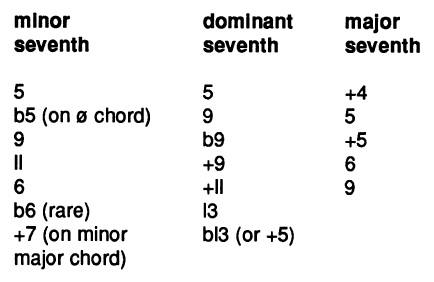
\includegraphics[width=3.1in]{levineextensions.jpg}
\end{figure}
There are a variety of ways through which it might be possible connect this simple model to jazz performance data.  Translated into corpus-analytic language, these traditional chord-quality voicing rules can be tested against the data of the Yale Jazz MIDI Piano (YJaMP) corpus.  An algorithm may look for root-third-seventh voicings (with various added tones) as signs standing for the seventh chords Martin places at the bedrock of jazz syntax.

In the presence of possible added tones, root determinations may be ambiguous or impossible to automate (or even hand-annotate consistently).  To sidestep this issue, I ask a simpler but analogous question: what chords occur in the YJaMP corpus which contain the three identifying chord tones listed above voiced in root-third-seventh ascending register within an octave?  For example, using a labeling system in which voicings are described by their semitonal distances above the bass note, what kinds of voicings contain $[0,4,10]$?

\begin{table}
\caption{Frequently-occurring corpus slices including $[0,4,10]$ voicing subsets.  These primarily include traditional dominant seventh chords with various added tones.  Note the traditionally unexpected appearance of $[0,4,10,17]$.  On what basis do we teach students to ``avoid" this natural 11?  What is its nature?}
  \centering
\begin{tabular}{l | l | l}
\hline\hline
Voicing & Counts & Additions \\ [0.5ex]
\hline
$[0, 4, 10]$ & 358 &  \\ 
$[0, 4, 10, 19]$ & 62 & add \nth{5} \\ 
$[0, 4, 10, 22]$ & 52 & double \nth{7} \\ 
$[0, 4, 10, 15]$ & 42 & $\sharp$\nth{9} \\ 
$[0,4,10,16]$ & 41 & double \nth{3} \\ 
$[0,2,6,12]$ & 40 & double \nth{7} \\ 
$[0,4,7,10]$ & 36 & add \nth{5} \\ 
$[0,4,10,21]$ & 36 & add \nth{13} \\ 
$[0,4,10,14]$ & 30 & add \nth{9} \\ 
$[0,4,10,13]$ & 29 & add $\flat$\nth{9} \\ 
$[0,4,10,17]$ & 23 & add \nth{11} \\ 
$[0,4,10,20]$ & 21 & add $\sharp$\nth{5} \\ 
$[0,4,10,18]$ & 21 & add $\sharp$\nth{11} \\ 
$[0,4,10,26]$ & 20 & add \nth{9} \\ 
$[0,4,10,28]$ & 20 & double \nth{3} \\[1ex]
\hline
\end{tabular}
\label{[0,4,10]}
\end{table}

Table~\ref{[0,4,10]} lists the most frequent voicings with dominant-seventh subsets.  To minimize reductive assumptions about non-harmonic tones, I search through ``salami slices" advocated by White and Quinn, verticalities generated from a na\"{i}ve approach agnostic about which pitches in a given stack should or can be disregarded.\footnote{For a full treatment of salami slice ideology, see \cite{wq2017}.}  As an algorithm thinly ``slices" the YJaMP performance corpus, it tracks each appearance and disappearance of a pitch, treating each resulting verticality as a potential chord, regardless of its pitch content.\footnote{White and Quinn trace their use of salami slices to comments by Ligeti; see \cite{wq2017}.} The most frequent chord additions match recommendations like those of Figure~\ref{levineextensions} almost precisely: chord tones like root, third, fifth, and seventh are added or doubled; diatonic extensions like 9 and 13 are added; alterations like $\sharp 9$, $\flat 9$, $\sharp 5$, and $\sharp 11$ are common.  The only place where the table of common voicings appears to disagree with received wisdom is in the frequent appearance of $[0,4,10,17]$, an apparent natural 11 chord.  What is the status of this observed sonority?

Levine, among many others, advocates against the ontological primacy of such sonorities.  Giving an explicit reason to discount this ``unusual" chord (but frequent slice) requires a kind of two-step ideological appeal to reduction like the following:
\begin{enumerate}
	\item This chord contains a dissonant or quality-ambiguating minor 9th between its third and eleventh, rendering it problematic and giving it some kind of unstable acoustical status.
	\item The chord cannot fulfill its usual harmonic function as is: instead, it likely functions as some kind of passing or neighboring chord in the context of a less-problematic, more-normative dominant sonority.
\end{enumerate}
A corpus-supported analog to step (1) is unclear, and it would likely fall prey to Gjerdingen's analyst-bias objections.  Claims of problematic consonance and dissonance would require psycho-acoustical modeling, appealing to measurable properties of sounded chords and human responses to them.  Such studies are more common in the classical literature, but some jazz work in this direction has begun to appear.\footnote{The auditory perception foundations of this kind of work stretch back to \cite{helmholtz1863}.  For an overview of sound  and critical band hearing research from the first half of the twentieth century, see \cite{scharf1961}; the later work of Plomp and Levelt aims this apparatus toward tonal consonance (see \cite{plomp1965}).  \cite{longuet1979} is emblematic of the turn taken when computational resources meet acoustics in a musical context, while a thorough treatment of modern psychoacoustics in common-practice classical music theory can be found in \cite{parncutt2012}.  \cite{mcgowan2008} engages with Helmholtzian perception in the context of jazz consonance and dissonance, but it draws on few of the empirical or computational tools of the above sources.}  Any corpus analytical claim regarding the impact of acoustical consonance on chord usage, if not accompanied by psycho-acoustical justification, would encode the analyst's expectations regarding jazz syntax into the data selection process, biasing any results meant to indicate how voicings appear in the corpus.  Pitch-based corpus statistics regarding which voicings are most common or important cannot be filtered for psycho-acoustic properties without biasing the results toward the whatever preconceptions the analyst chooses to encode.

A corpus of performances can be made to suggest lines of reasoning like (2); a tally of what kinds of voicings tend to follow $[0,4,10,17]$ provides a cursory suggestion as to its use.  If this voicing tends to progress to subsequent harmonies in a way strongly similar to (or different from) other dominant voicings, it may (or may not) stand in for Martin's dominant seventh chord category, despite Levine's intervallic contraindications.

Figure~\ref{[0,4,10,17]} shows the most common voicing salami slices to appear within 50 slices of $[0,4,10,17]$.\footnote{Note that this flexible span reflects the appearance or disappearance of any single note 50 consecutive times.  At extremely quick tempos or during fast runs, 50 slices could pass in a couple of seconds; at slow tempos or during moments of stasis, the same number of slices might cover tens of seconds (or, formally, an arbitrarily long time).}  Each destination slice is indexed here by both its semitonal voicing structure and the number of semitones its bass lies above or below the bass note of $[0,4,10,17]$.  For example, the most common nearby destination slice is the voicing $[0,1,5]$, the seventh, root, and third of a major-seventh chord in registrally-ascending order (see the yellow line in Figure~\ref{[0,4,10,17]}). The seventh of this destination chord (found in the bass) lies a major third above the bass of the preceding $[0,4,10,17]$ chord (hence the initial 4-semitone entry in the relevant parenthesis).  While the slice counting algorithm has made no assumptions of any kind about key, this ``progression" implies traditional root motion down by fifth, indicating that $[0,4,10,17]$ most frequently appears in the context of dominant-tonic motion.  Crucially, this dominant-tonic motion typically occurs on a time scale of many (18-30) slices; during that span, the ``unusual" voicing has plenty of opportunities to ``resolve" or clarify its status: melodic motion might connect it to a more normative dominant-seventh, like $[0,4,10,14]$, or a consonant dominant triad, like $[0,16,19]$ (see the blue line in Figure~\ref{[0,4,10,17]}).  Due to the wide variety of destination voicings found after $[0,4,10,17]$, this is comparatively weak support for the two-step reduction outlined above, but it does indicate the form such an appeal might take in corpus analytic terms.  An analysis based solely on voicing structure produces an observation defying the properties of the voicing model, so the analyst turns to some behavioralist reduction criteria to normalize the results.

\begin{figure}
	\caption{Following slice behavior for $[0,4,10,17]$ voicings.  The voicing appears most frequently in the neighborhood of $[0,1,5]$ voicings a major third up (yellow line), implying its participation in $V^7 \rightarrow I^2$ dominant-tonic progressions.  But salami slice adjacencies also imply intra-syntactic progressions at shorter scales; the blue line plots the appearance of $[0,16,19]$, the dominant triad sharing a bass note and root with the preceding $[0,4,10,17]$.}
	\label{[0,4,10,17]}
	\centering
	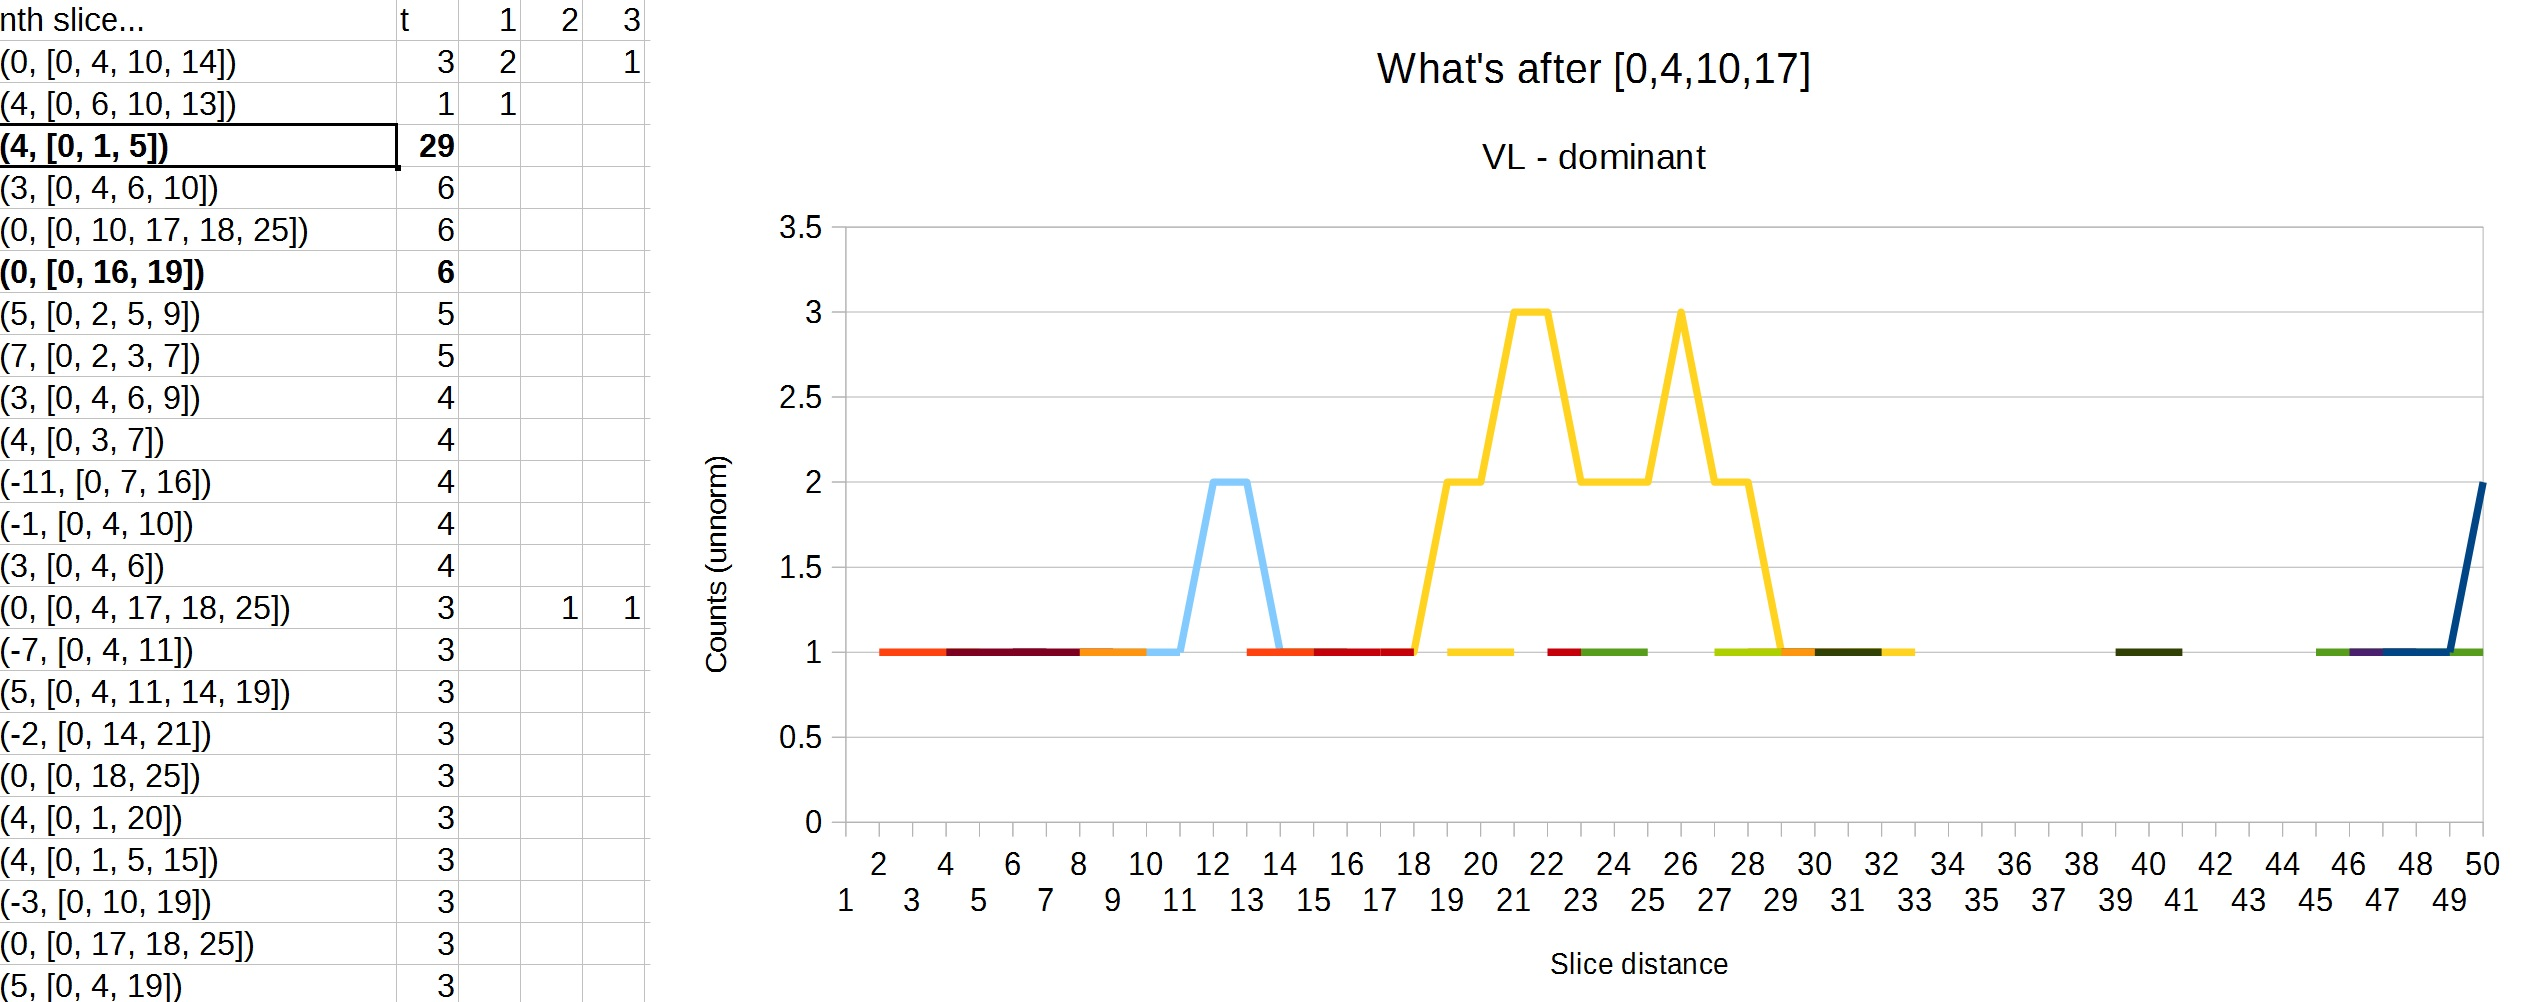
\includegraphics[width=6in]{041017_behavior.jpg}
\end{figure}

This procedure relies on a particular type of descriptive and explanatory model, and it still encodes analytical (and ontological) preconceptions regarding chord structure and harmonic progression.  To produce claims of this kind, there must exist a small number of frequently-employed chords of some ideologically-approved structure (i.e., seventh-chords with approved extensions and alterations) and a set of reduction techniques designed to render sounding sonorities of other types analytically (or at least syntactically) unimportant.  Identifying a voicing and deducing the properties of voicing types requires some minimal ontological framing, and other harmonic tasks may or may not be possible within the same frame.

\section{Selecting Objects of Harmonic Significance}
%Introduce and unpack Kockelman's semiotic diamond
The analytical pathway from abstract seventh chords to actual voicing statistics given in the preceding section relies on a selection process similar to those captured by \cite{kockelman2013} in his Figure 2.6, reproduced as Figure~\ref{kockelman} below. 

\begin{figure}[h]
	\centering
	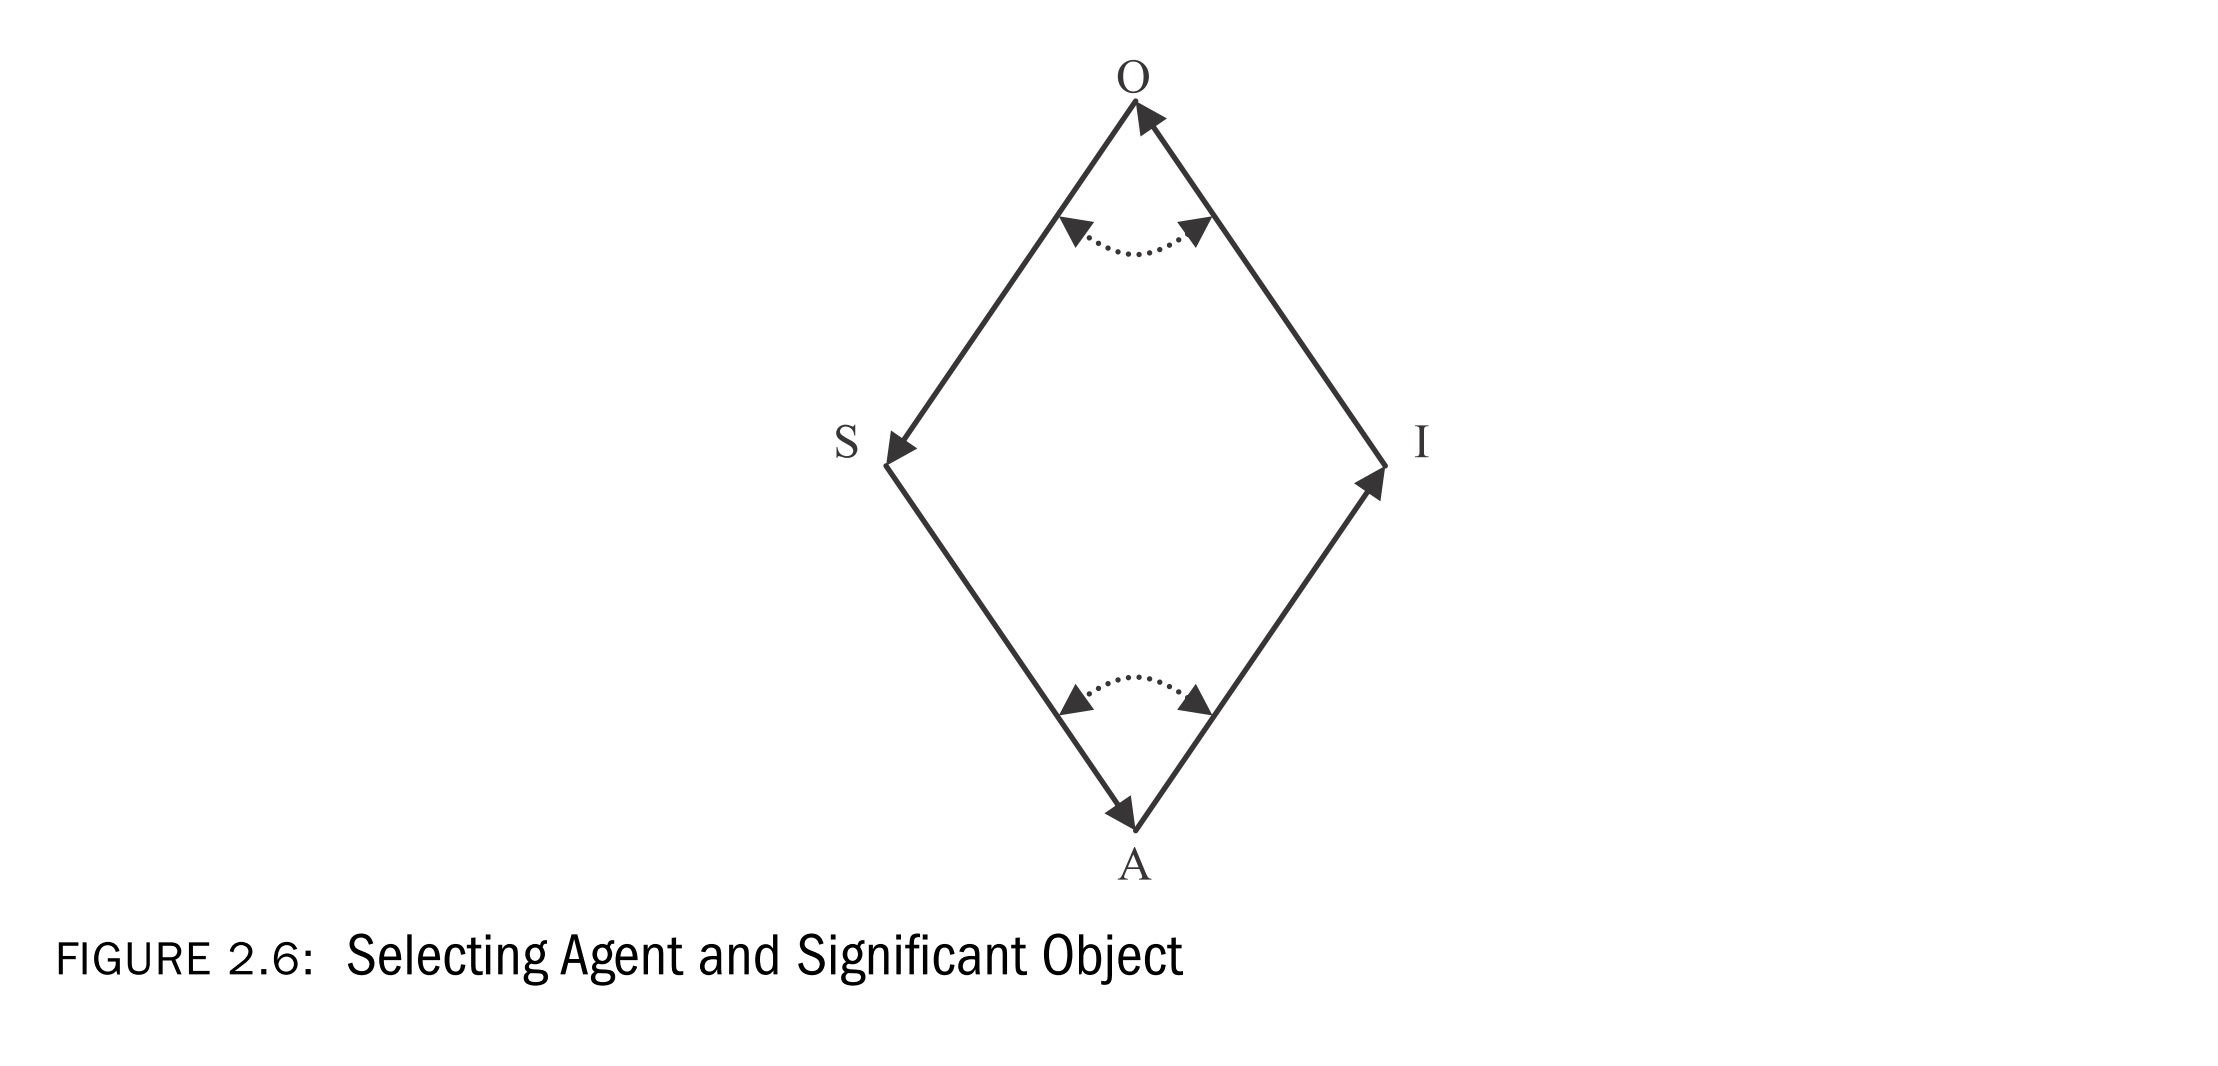
\includegraphics[width=6in]{kockelman_model.jpg}
	\caption{Figure 2.6 from \cite{kockelman2013}, a general model for the ``relation between relations" inherent in selection.  The significant object (O) and selecting agent (A) are codetermined by their relations to observable signs (S) and resulting interpretants (I).}
	\label{kockelman}
\end{figure}

This figure diagrams a flexible kind of ontological framing for semiotic processes involved in labeling, interpretation, and analysis in general.  At the top and bottom corners of this diamond, music analysis like that of the previous section places the abstract chord objects ($O$) postulated as harmonic categories (like Martin's ontologically-basic seventh chords) and the analytical agent seeking to identify, transform, and react to those objects ($A$).  The analyst does not observe the postulated objects ($O$) directly, but rather through certain traces or signs ($S$) found in the performance data, whether the engagement with those performances is acoustical (for a listening agent or pianist), visual (for a score analyst), or digital (for a corpus analyst).  The analyst observes these signed traces and produces interpretants ($I$) that make sense given the presumed existence of $O$.  These interpretants might be roman numerals that an analyst assigns to particular sonorities to represent the category of harmonic object to which they belong, or they may be expectations regarding subsequent objects which might be sounded in a performance, among other possibilities.

In a very basic analysis, the analyst might encounter a root-third-seventh voicing like $[0,4,10]$ and interpret it as a sign $S$ for an abstract (and inherently unobservable) ``dominant seventh chord" object $O$.  The analyst might then apply a roman numeral interpretant like $V^7$ to a particular location in the score and begin looking for the next syntactically-appropriate chord.  For Kockelman, the interpretant ``makes sense in the context of $S$ from the standpoint of $A$."\footnote{\cite{kockelman2013}, p.\ 17.}  The agent/analyst $A$ selects certain indices $S$ by turning signs into actions.  But Kockelman also describes the properties of the \emph{object} through a parallel and codetermined process: just as the interpretant $I$ makes sense from the standpoint of $A$ in the context of $S$, ``$I$ makes sense in the context of $S$ given the properties of $O$."  Here, $V^7$ only ``makes sense" in the context of $[0,4,10]$ if the roman numeral object has properties like identifiable root, chord structure, relationship to a key, surface segmentation, and so forth.  The resulting ``relation between relations" (the dotted lines of Figure~\ref{kockelman}) underpins semiotic processes of selection and significance, since the sense-making of $I$-given-$S$ requires and produces both a selecting agent and a significant object -- though the ontological structure from which the object $O$ arises can only be accessed, described, or interpreted by $A$ indirectly, through actions based on signs.

The flexible framework of Figure~\ref{kockelman} applies to a huge variety of selection processes, including many contexts where musical actions are taken.  In the case of actual performance, a jazz vocalist may interpret heard sonorities $S$ as indicating that a pianist is playing a kind of dominant seventh chord object $O$, and the vocalist might then choose to sing certain notes well-suited to that chord and expect and prepare for certain kinds of (say, tonic) sonority to sound after a particular time delay.  The fact that these actions make sense from the perspective of the singer (given the original heard sonority) is thoroughly entangled with the fact that the resulting actions make sense with respect to the properties of $O$ given the presence of $O$'s significant indices $S$.

Crucial to Kockelman's description of selection and significance is the claim that all agents performing (re)actions \emph{must do so under some ontological assumptions}, whether they are conscious or unconscious, enminded or embodied.  For an analyst to assign a roman numeral to a sonority, the analyst must partake of an ontology in which a variety of sonorities map to each roman numeral on the basis of their pitch class content as tokens of a type or individuals of a kind.  The analyst's interpretant (i.e., ``$V^7$," or ``look for a subsequent tonic") makes sense if and only if the kind ``dominant seventh chord with a root on scale degree five" has properties underpinning the identification of sonority/sign $S$. To use recursive language echoing Kockelman's own descriptions, the relation between the analyst-interpretant relation and the sign-analyst relation mirrors the relation between the interpretant-object relation and the object-sign relation.  Selecting a labeled kind correlated to a set of signed indices relies on and produces an ontological system.  

%Modes of ontological transformativity
Kockelman's careful attention to signed indices and acted interpretants as integral components of semiotic processes allows him to typologize their potential ontological impacts.  Consider three ``modes of ontological transformativity," to adapt part of Kockelman's typology to a music-analytical case:\footnote{The most direct analog to this discussion surrounds Table 1.2 in Chapter 1 of \cite{kockelman2013}.}
\begin{enumerate}
	\item The presence of certain notes in a voicing may change the analyst's ontological assumptions about what kinds constitute and apply to the individual sonority: ``The sign $[0,4,10]$ makes me think this sonority is a dominant seventh chord."
	\item The presence of certain notes in a very large number of similar voicings may change the analyst's ontological assumptions about what notes or intervals make up a particular kind: ``Many sonorities seem similar to $[0,4,10]$ in some important way but carry indices $[0,4,10,15]$, so perhaps a property of dominant seventh chords as a kind is that they may contain a $\# 9$ above the bass."
	\item The presence of certain unfamiliar voicings in frequent but unfamiliar patterns may change the analyst's assumptions about what voicings and harmonic objects make up a particular style or musical world: ``Many voicings do not neatly align with qualities of seventh chord, so perhaps seventh chords are not the objects (or are not the \emph{only} objects) I should react to or label."
\end{enumerate}
Transformations of type (1) here correspond most directly to undergraduate-style harmony assignments, where student analysts map observed traces to stable, received chord categories.  Transformations of type (2) constitute much of the academic music theory literature, where professional analysts logically induce pitch-based patterns of behavior from a particular corpus given a mostly-stable set of ontological kinds.  Both of these modes of ontological transformativity are well-suited to corpus analysis relaying on the ``numerical methods and explicit algorithms" Gjerdingen describes as appropriate for two-thirds of his recipe.  Gjerdingen's bias objection primarily concerns transformations of type (3), where the categories signed and represented by the statistically-tallied indices themselves change.  And the avoidance of such changes is impossible, since selecting agents produce and are imbricated in their own ontologies -- to get any selection and response procedure off the ground, the analyst must encode some set of ontological assumptions.  Where Gjerdingen says this reveals a ``presentist or historicist bias," we might say that this reveals the necessity (and inescapability) of ontological framing in analytical processes.

%aligning relations between relations
If the properties of the object ($O$) and the actions of the agent ($A$) are entangled across a semiotic process of selection and significance, the signed indices ($S$) to which the agent reacts ($I$) may be framed in a variety of ways; analysis will not consist of unearthing pre-existing harmonic objects, but rather of framing a harmonic ontology in which the properties assigned to chord objects align with the interpretants produced by the agent(s).  Different agent-interpretant relations -- different types of action or expectation taken or embodied by the analyst -- may relate more directly to certain kinds of object-sign relation than to others.  This alignment of relations between relations guides the framing of this dissertation and results in a close focus on the relays between computational category formation and temporal statistics.

\section{Harmonic objects and interpretants}
%lay out several analytical interpretants and the object-sign framings best related to them
Modes of harmonic analysis with different interpretants and objects can be framed accordingly.  Four are shown in Table~\ref{frames}.
\begin{table}%[h]
  \caption{Four framings of harmonic analysis generating (and requiring) different semiotic ontologies.}
  \centering
\begin{tabular}{>{\raggedright}p{1.6in} |>{\raggedright}p{1.8in} | >{\raggedright\arraybackslash}p{1.8in}}
\hline\hline
Interpretant & Signed Indices & Harmonic Object \\ [0.5ex]
\hline
Identifying a voicing structure & Intervals above the bass at a particular time & Pitch verticalities \\ \hline
Postulating a scale & Pitch class frequencies over time & Macroharmonic collections \\ \hline
Assigning a traditional roman numeral & Keys, pitch-class sets, reduction rules & Tertian scale degree stacks \\ \hline
%Choosing a key & Scales and articulated centricity & Tonics and modes \\
Interpreting a chord's syntactic function & Scale degree sets over time & Categories of similar scale degree sets \\[1ex]
\hline
\end{tabular}
\label{frames}
\end{table}
An analyst seeking to identify a type of voicing, following the directions of Martin and Levine, assumes (and produces) a class of pitch verticalities ($O$); the decision to place a given sonority into such a class (be they quality-based, cardinality-based, or otherwise) makes sense to the analyst given its intervals above the bass ($S$) and the existence of voicing classes ($O$) with certain intervals above the bass as properties.  This analytical process requires minimal temporal data, as the sonority's voicing structure can be gleaned from an extremely brief snapshot of a score or fragment of an audio recording, but it still assumes some temporal properties as the basis for its ontology: voicings as pitch verticalities are typically represented as simultaneities, when actual performance traces will surely exhibit slight onset time differences between each of the notes ``in" a voicing.

On another temporal scale, an analyst postulating a scale underpinning a certain passage of music assumes (and creates) limited macroharmonic collections of pitch classes that can be related to musical surface signs in particular ways; if pitch-class distributions can lead the analyst to produce a scale, then the scale object can be given such a surface distribution as a property or signed index.  In this case, as in the voicing case, the method by which the agent produces an interpretant from signed indices aligns with the properties assigned to the objects in the resulting semiotic ontology.

To assign a roman numeral or interpret a chord's syntactic function requires a more complex ontology, where the semiotic relations between the objects' properties and the agents' interpretants become less direct.  For a traditional roman numeral to ``make sense" to an analyst, she must postulate the existence of keys and pitch-class sets standing in some relation to one another.  To label the (untransposed) pitch class set $[0,4,10]$ as $V^7$ is also to assume (or create) a kind, ``$V^7$," connected to signed indices in some meaningful way.  The nature of this connection, the sense-making of ``$I$ in the presence of $S$ given the properties of $O$," is codeterminate with the with the sense-making of ``$I$ in the presence of $S$ from the perspective of $A$."  The precise way in which the analyst turns surface signs into interpretants (analytical symbols and expectations) may be thought to generate (and respond to) the way harmonic object categories relate to their signed indices (pitch and temporal properties) -- undermining any assumptions regarding the ``real" or analyst-independent nature of chord categories $O$.

On this basis, roman numeral analysis as an interpretive act fractures into several separate semiotic processes with their own distinct ontological conditions.  If the analytical interpretant produced ($V^7$) makes sense to analyst $A$ because it consists of a tertian stack of dominant seventh quality built on scale degree $\hat{5}$ of the local key, then the semiotic kind to which the individual sonority has been assigned carries properties based solely on its pitch class structure and relation to a key.  But if the same analytical interpretant is produced through some other relation to pitch and time indices, the kind $V^7$ may participate in an entirely different ontology permitting entirely different properties and modes of proof.  In particular, if $V^7$ makes sense to analyst $A$ \emph{because the observed sonority ``behaves like" other chords of kind $V^7$}, the ontological structure embedding the kind $V^7$ changes quite radically.  The relation between kind $V^7$ and its indices can no longer be captured by pitch class structure and key relation; instead, it requires additional -- and potentially conflicting -- knowledge about temporal progression or syntactic function.  As the last line of Table~\ref{frames} indicates, the interpretation of a chord's syntactic function treats more than a sonority's pitch structure as indices; such an interpretant also involves the agent's knowledge regarding what chords tend to succeed the given sonority at certain time scales.

The same human analyst may produce interpretants over-determining the properties assigned to harmonic categories at various levels of ontological transformativity.  Observing a chord's pitch-class structure or that it almost always precedes a stable tonic might lead the analyst to recognize it as part of the kind $V^7$, an ontological transformation of mode (1) above.  Or the repeated observation of those indices might lead the analyst to decide that they stand as properties of the kind $V^7$, a mode (2) transformation.  Or the analyst's concern that many chords which display some of the expected indices but not others (say, common progression behavior but unfamiliar pitch class structure) might lead to a re\"{e}valuation of the ontology framing the kind $V^7$, producing a kind category at a higher (or overlapping!) ontological level like ``dominant function," where progression behavior constitutes the signed indices producing interpretants, relegating exclusively pitch-structural indices to kinds like $V^7$.  In such an ontology, interpretive acts like ``this chord is a $V^7$" and ``this chord has dominant function" would partake of separate ontologies, rely on distinct types of evidence, and involve different analytical skills.

%transition to particular corpus-analytical harmonic analysis framings.
Some of the most-maligned limitations of computational methods -- their blessed ignorance of musical context and their blind reliance on the digital representation of the corpus -- can prove crucially useful for the generation of particular and consistent semiotic ontologies.  While human-generated interpretants like ``this sonority is a $V^7$" or ``this chord typically precedes tonic" can reference categories over-determined by their relation to indices of varying modality, algorithmic statistics and machine learning methods can be forced to produce interpretants which make sense only and precisely in the context of particular sets of indices.  With a Python implementation of an algorithm as agent $A$ in Figure~\ref{kockelman}, the direct relation between the sense-making of $I$ in the presence of $S$ from the perspective of $A$ and the sense-making of $I$ in the presence of $S$ given the properties of $O$ is strictly enforced.  The algorithm can only assign properties to object categories based on the input indices it observes -- it knows no other possible features of the object than the signs encoded in the corpus's representation.  

The remaining sections of this chapter provide examples for how such algorithmic work might ``object"-ify the YJaMP corpus.  Given interpretants designed to operate at different time scales and with different analytical aims, different computational processes are employed to ensure that the interpretant-agent-sign relations are precisely co-generated with the interpretant-object-sign relations.  The categories used to describe harmonic objects in the corpus generate different ontologies in different analytical circumstances.  Statistics regarding voicings and scales suggest future analytical projects based on YJaMP or other corpora, while temporal encodings of scale degree sets lay the groundwork for the generalized harmonic progressions of chapter 3 and the syntactic category formation of chapter 4.
 
\section{Voicings revisited}
%voicings in general, supporting and complicating Levine with more ontology
To return to the voicing statistics of Tables~\ref{[0,4,10]} and \ref{[0,4,10,17]}, we can now distinguish their different framings.  In the first case, the algorithm-as-analyst produced frequency statistics of different $[0,4,10]$ superset voicings as interpretants.  As a necessary correlate to these statistics, it assumed (or created) an ontology of voicing objects with particular properties: members of the category tallied contain an $[0,4,10]$ pitch subset, where the sounding pitches necessarily overlap in time (though they need not all begin at the same moment).  There are many subtle consequences of this ontology, like the fact that it captures voicings which may not have traditional syntactic significance (like $[0,4,10,17]$), or that a particular voicing might belong to a large number of categories.  Tables~\ref{[0,4,11]} and \ref{[0,3,10]} provide other interpretants from within the same framing: frequently-occurring corpus slices containing $[0,4,11]$ (major seventh) or $[0,3,10]$ (minor seventh) subsets.  These statistics contain further ambiguities of the same kind, but they generally support the added voice instructions given by Levine, among others.

%Check the text for whether I cite/explain upper structure voicings?
\begin{table}
\caption{Frequently-occurring corpus slices including $[0,4,11]$ voicing subsets.  These include traditional major seventh chords with various added tones, but also other traditional (``sus") and non-traditional ($[0,6,10,17]$) chords.}
  \centering
\begin{tabular}{l | l | l}
\hline\hline
Voicing & Counts & Potential interpretation \\ [0.5ex]
\hline
$[0, 4, 11]$ &	197 & \\ 		
$[0, 4, 7, 11]$ &	144	& Add \nth{5}	\\ 	
$[0, 4, 8, 11]$	& 124	& Add $\sharp$5 or $\flat$6\\ 	
$[0, 4, 6, 11]$ &	115	& Add $\sharp$4	\\ 	
$[0, 4, 5, 9, 16]$ &	89	& \nth{2} inversion, add \nth{5}, doubled \nth{7}\\ 	
$[0, 15, 19, 22, 26]$ &	80	 & Minor \nth{7}, add \nth{9}\\ 	
$[0, 15, 19, 26]$ &	62	& Minor \nth{7}, add \nth{9}\\ 	
$[0, 5, 9, 16]$ &	61	& \nth{2} inversion, add \nth{5}	\\ 	
$[0, 1, 5, 12]$ &	57	& \nth{3} inversion	\\ 	
$[0, 6, 10, 17]$ &	57	& (?)	\\ 	
$[0, 16, 20, 24, 27]$ &	52 & US $\flat$VI	\\ 	
$[0, 4, 8, 12, 15]$ &	51	& US $\flat$VI	\\ 	
$[0, 10, 14, 17, 21]$ &	49	& Sus chord	\\ 	
$[0, 10, 14, 21]$ &	48	& Sus chord	\\ 	
$[0, 8, 12, 16, 19]$ &	45	& (?)\\ 	
$[0, 2, 4, 11]$ &	44 &	Add \nth{9}	\\ 	
$[0, 10, 14, 18, 21]$ &	38 & US II	\\ 	
$[0, 1, 5, 8, 12]$ &	38 & Doubled \nth{7}\\[1ex]	 
\hline
\end{tabular}
\label{[0,4,11]}
\end{table}

\begin{table}
\caption{Frequently-occurring corpus slices including $[0,3,10]$ voicing subsets.  These include traditional minor seventh chords, with various added tones, as well as several voicings of ``sus" chords.}
  \centering
\begin{tabular}{l | l | l}
\hline\hline
Voicing & Counts & Potential interpretation \\ [0.5ex]
\hline
$[0, 3, 10]$ &	198	& \\ 
$[0, 7, 10, 17]$ &	93	& Sus\\ 
$[0, 3, 7, 10]$ &	91	& Add \nth{5}\\ 
$[0, 3, 5, 10]$ &	84	& Add \nth{4}(?)\\ 
$[0, 7, 10, 14, 17]$ &	58	& Sus\\ 
$[0, 4, 7, 14]$ &	46	& Major \nth{7}, add \nth{9}\\ 
$[0, 2, 5, 12]$ &	41	& Doubled \nth{7}\\ 
$[0, 7, 10, 12, 14, 17]$ &	41	& Sus\\ 
$[0, 7, 10, 14, 15, 17]$ &	39	& Minor \nth{11} or Sus\\ 
$[0, 3, 10, 15]$ &	38	& Doubled \nth{3}\\ 
$[0, 3, 10, 17]$ &	32	& \nth{11}\\ 
$[0, 3, 5, 7, 10]$ &	29	& Add \nth{4}(?)\\ 
$[0, 3, 7, 10, 14]$ &	29	& Add \nth{5} and \nth{9}\\ 
$[0, 16, 19, 23, 26]$ &	28	& Major \nth{9}\\ 
$[0, 3, 10, 14]$ &	28	& Add \nth{9} \\[1ex]	 
\hline
\end{tabular}
\label{[0,3,10]}
\end{table}

The categories produced by the algorithmic statistics carry no necessary syntactic properties, since the tallying process relied only on snapshots pitch alignment in time.  Even the quality of the resulting sonorities cannot be consistently determined; without knowledge of the local key and harmonic context, the root of a voicing like $[0,4,8,11]$ from Table~\ref{[0,4,11]} could be the bottom voice (0), in which case the chord contains a major third (4), sharp fifth (8), and major seventh (11), or it could be the second from bottom voice (4), in which case the chord contains a major third (8), perfect fifth (11), and flattened sixth (0).  There are good reasons to prefer the former interpretation over the latter, but the flexibility of tertian-stack quality and root identification renders both possible.  Since the voicing tally algorithm knows nothing about root or quality label, it remains agnostic regarding many potential chord properties: membership in the superset voicing category $[0,4,11]$ does not require major seventh quality, any particular root, or any particular syntactic function.

The category membership nevertheless implies some of those properties to a human analyst in a productive way, but this is to partake of a separate semiotic process diagrammed in Figure~\ref{kockelman_2dia}, taken from \cite{kockelman2013}.  The tallying algorithm $A_1$ observes voicing indices $S_1$ and produces superset statistics $I_1$ which make sense given the intervallic properties of the shared subset being tallied $O_1$.  The subsequent human analyst $A_2$ observes voicing superset statistics $S_2 = I_1$ and produces interpretants $I_2$ (like the quality label ``major seventh chord") which make sense in the context of the voicing statistics \emph{and} some embodied or enminded assumptions regarding root assignment or voice-leading reduction.  Since these properties are involved in $A_2$'s production of $I_2$, we might view them as generating signed objects $O_2$ with entirely different properties from $O_1$.  The communication between algorithmic agent and human agent can (or perhaps \emph{must}) produce different ontological framings.

\begin{figure}%[h]
	\caption{Figure 2.7 from \cite{kockelman2013}, a doubly-semiotic model for ``communication between conspecifics."  If $A_1$ and $A_2$ are a voicing tally algorithm and a human analyst, the statistical point of intersection $I_1 = S_2$ connects two processes generating different objects $O_1$, $O_2$.}
	\label{kockelman_2dia}
	\centering
	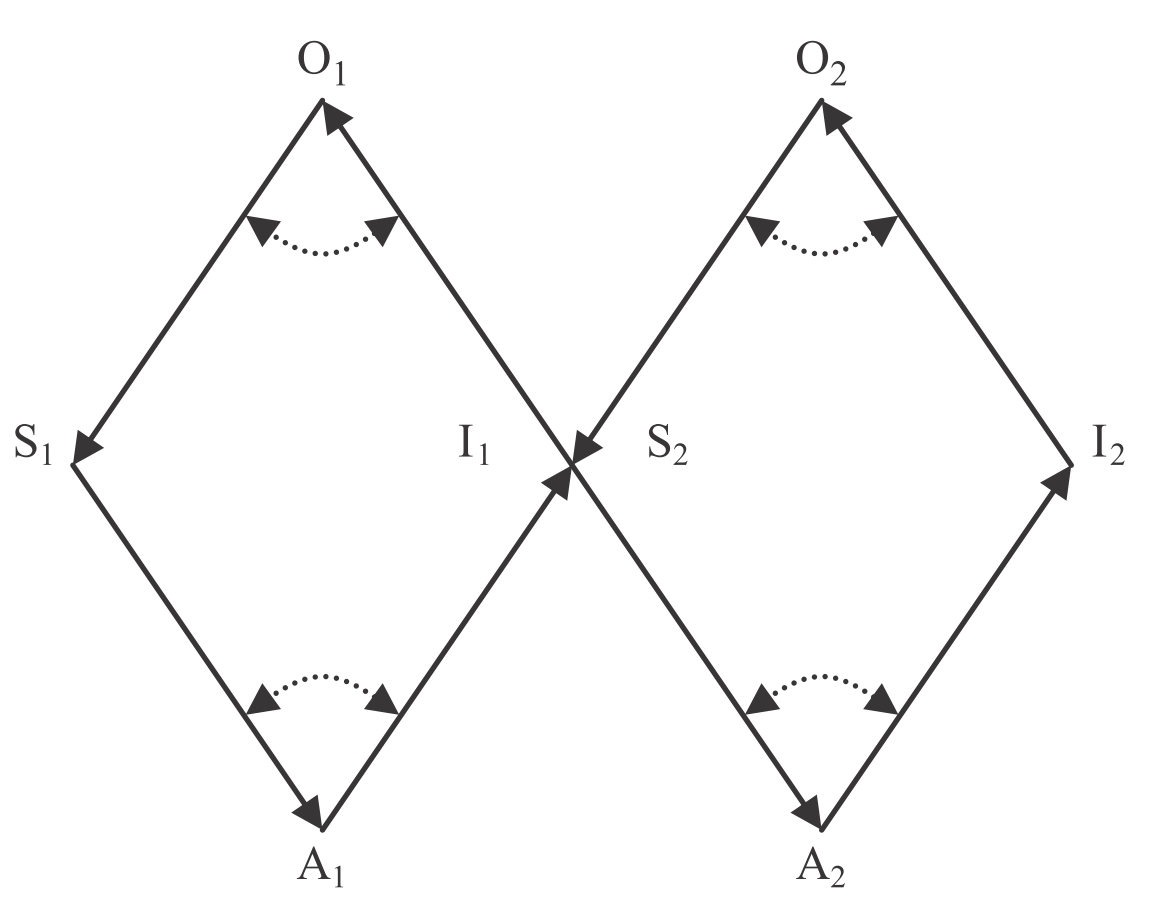
\includegraphics[width=3.5in]{kockelman_2dia.png}
\end{figure}

The potential for misinterpretation here, for ``parasitic" processes redirecting $I_1$ to some end quite different from that intended or produced by $A_1$, is clear, and it is under this condition that human-run corpus analysis must operate.\footnote{In Kockelman's terms, parasitic processes redirect or reframe semiotic processes in a variety of ways.  As formalized on \cite{kockelman2013}, p.\ 15, an object ``considered as a means to an end" (that is, as a tool for mapping $S$ to $I$) ``is a second (or an intermediary), but insofar as it implies (embodies or indexes) other ends it might be directed to serve... it is a third (or mediator).  The parasite is whatever inhabits such implications."  I will return to the implications of this claim in the concluding chapter.}  The above statistics for root-third-seventh voicing subsets imply that Levine's added tone descriptions are apt, but the price of escaping circularity in data selection is ontological instability.

Just as na\"{i}ve voicing superset tallies can be made to lend performance data driven support to three-note voicing and added tone prescriptions, the same algorithm can connect Levine's ``A" and ``B" left-hand voicings to potential chord qualities.  In Chapter 7 of his \emph{Jazz Piano Book}, Levine formalizes a harmonic progression technique designed to project $ii$-$V$-$I$ chord qualities through efficient voice leading within a single (typically left) hand voicing.  Compacting the chord changes into a single hand ``gives your right hand the freedom to play the melody or improvise," and Levine cites their occasional use by Tatum, Garner, Jamal, and Garland and attributes their codification to Bill Evans and Wynton Kelly.\footnote{\cite{levine1989}, p.\ 41.}  The left-hand voicings (LHV) present a challenge to traditional tertian-stack analysis, since they lack what Levine perceives to be the ``root" of each chord.\footnote{This is not to say that no theoretical justifications for the LHV in tertian contexts exist in the literature; Levine himself offers specific contextual justifications, while Quinn provides a general framework flexible enough to account for the LHV with generic intervals and contrapuntal rules (see \cite{quinn2017}, \S 4).}  While a bass player may pick up the roots during combo gigs, the LHV have nevertheless become a fixture of solo piano performance, and they appear frequently in the YJaMP corpus.  The two sets of efficient LHV from Levine's chapter seven are reproduced in Figures~\ref{levine_Avcg} and \ref{levine_Bvcg}.

\begin{figure}%[h]
	\caption{The ``A" left-hand voicings from Figure 7-2 of \cite{levine1989}.}
	\label{levine_Avcg}
	\centering
	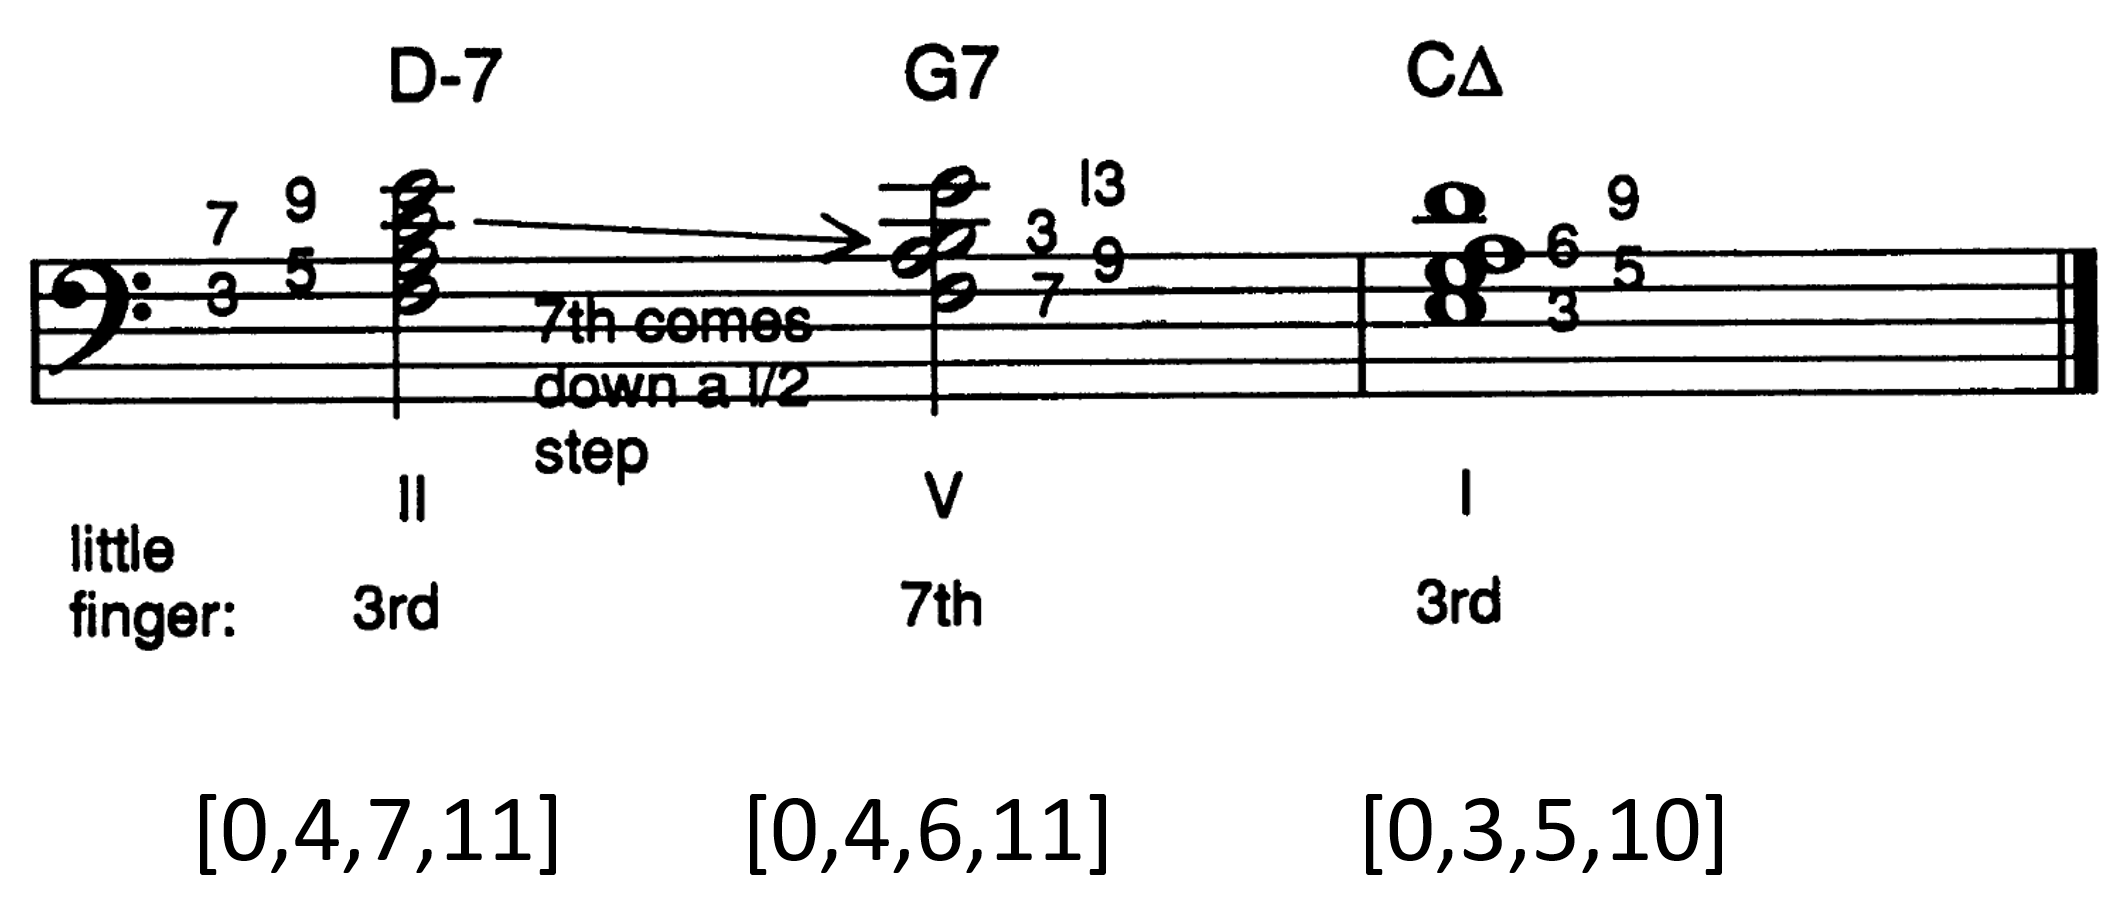
\includegraphics[width=4in]{Levine_Avoicings.png}
\end{figure}
\begin{figure}%[h]
	\caption{The ``B" left-hand voicings from Figure 7-4 of \cite{levine1989}.}
	\label{levine_Bvcg}
	\centering
	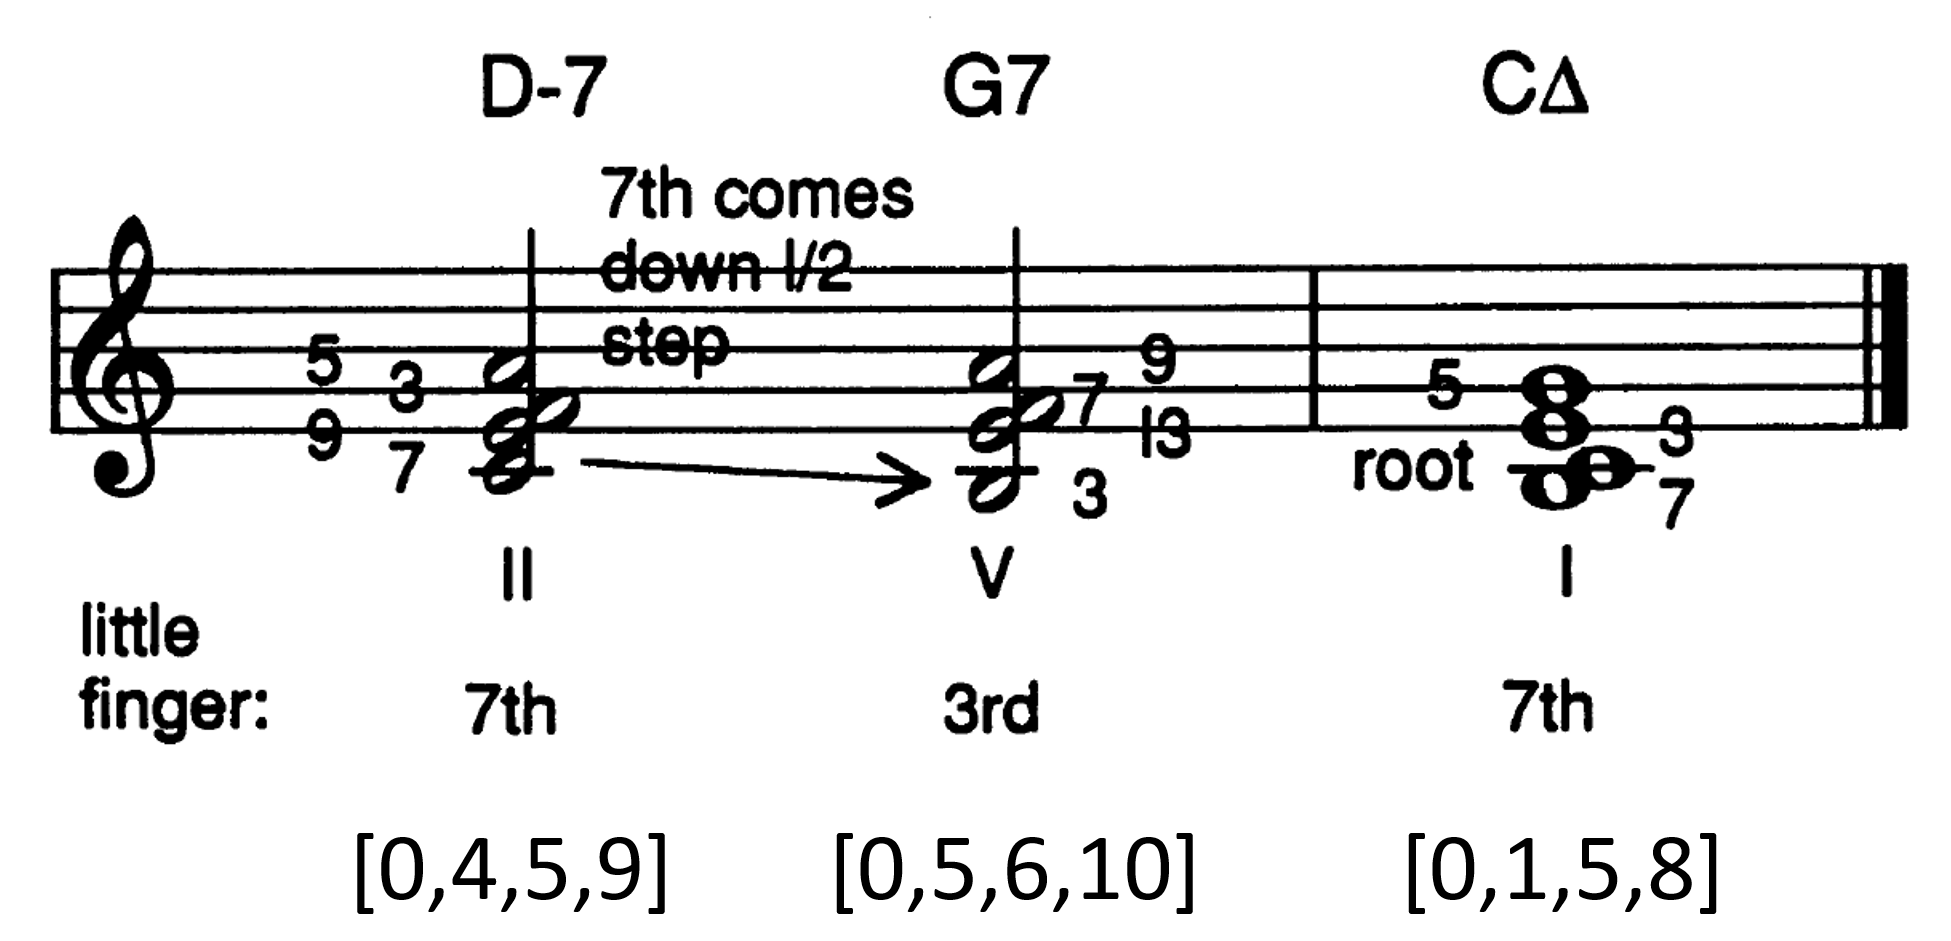
\includegraphics[width=4in]{Levine_Bvoicings.png}
\end{figure}

The intervallic structures of the A and B voicings differ from the qualities of the chords Levine intends them to index, represent, or support.  The $FM^7$ chords meant to be played in the syntactic context of ``$D-7$" can be represented with semitonal voicings $[0,4,7,11]$ and $[0,4,5,9]$, and the $G7$ voicings lack a $G$ but sound the appropriate $BF$ tritone alongside presumed chordal 9ths and 13ths.  Levine's imagined pianists run the semiotic analytical process backwards, in a way: the pianist $A$ sees chord symbols like $D-7$ or $G7$ on a lead sheet and produces voicings as interpretants.  These voicings make sense in the context of the chord symbols from the perspective of the pianist given categorical objects signed or indexed by the chord symbols: $D-7$ and $G7$ must refer to flexible collections of notes or chords for which the A and B voicings serve as adequate (or at least acceptable) responses.  Pianist-analyst communication, along these lines, might be mapped back onto Figure~\ref{kockelman_2dia}; in the left diamond, the pianist $A_1$ turns lead sheet signs into voicings ($S_1 \rightarrow I_1$), while in the right diamond, the analyst $A_2$ turns voicings back into chord symbols of some kind ($I_1 = S_2 \rightarrow I_2$).  The alignment of the framed objects $O_1$ and $O_2$ depends on the particular ways in which $A_1$ and $A_2$ make sense of their interpretants within particular (and perhaps quite different) ontologies.

To attempt to tally the appearances of Levine's left-hand voicings in YJaMP is to interpose (at least) a third diamond -- and a third agent -- into the middle of the communicative semiotic chain.  Pianist $A_1$ turns many chord symbols into many voicings; algorithm $A_2$ turns many voicings into statistics regarding common supersets; analyst $A_3$ turns those statistics into observations regarding added tones, chord quality, and categories of substitutability.  Far from collapsing the distinction between $O_1$ and $O_2$, numerical models here multiply it.  We might be inclined to tack on yet another diamond before the others, where a tune writer turns imagined, composed, or improvised sonorities into lead sheet symbols-- in which case the entire communicative enterprise might suggest a kind of philosophical fictionalism, where each agent's actions are embedded in an ontology appealing to certain kinds of harmonic objects as a convenient way to facilitate the production and communication of their own interpretants.  Embracing a music theoretical fictionalism similar to Hartry Field's nominative philosophy of mathematics would amount to claiming that roman numeral models (or chord categorical claims, more generally) provide a reliable and convenient communicative framework consisting of literal falsehoods.\footnote{I note in passing that since music theory seems to rely more heavily on first-order logic than second-order, it may be a more appropriate domain for Field's construction than mathematics, the second-order logical constraints of which have generally limited Field's acceptance by the field.  See \cite{field1980}.}  To adopt complete skepticism regarding chord categories as referring to anything existing independently in the real world would amount to a very high mode of ontological transformativity, in Kockelman's terms.\footnote{While acceptance of this position is not strictly required by my project here, I align myself in this direction, and I think it can be read out of work like \S 1 of \cite{quinn2017}.}  All this to say: using corpus statistics to assess the appropriateness of the left-hand voicings as descriptors of piano performance is like standing on a stool balanced on a chair placed on a crooked floor.\footnote{Passionate defense or criticism of musical corpus analysis seems to depend on whether one thinks the analyst in this precarious position is trying to reach the ceiling or the floor.}  So it is deceptive and surprising how straight-forward the results appear.

\begin{table}%[h]
  \caption{Supersets of of Levine's $ii$ ``A" left-hand voicing (LHV) $[0,4,7,11]$.}
  \centering
\begin{tabular}{l| l | l}
\hline\hline
Voicing & Counts & Potential interpretation \\ [0.5ex]
\hline
$[0,4,7,11]$ & 199 & Major seventh or $ii$ LHV\\
$[0,15,19,22,26]$ & 117 & LHV + added root = minor ninth \\
$[0,10,14,17,21]$ & 58 & Major ninth in inversion, or sus? \\
$[0,1,5,8,12]$ & 51 & Major seventh with doubled 7 \\
$[0,2,4,7,11]$ & 47 & Major seventh add 2 \\
$[0,3,7,10,14]$ & 36 & LHV + added root = minor ninth \\[1ex]
\hline
\end{tabular}
\label{a_ii_lhv}
\end{table}

In Figure~\ref{a_ii_lhv}, I turn the superset voicing statistics produced algorithmically for all the appearances of $[0,4,7,11]$ corpus-wide into interpretations invoking chord quality and added tones.  The most frequent voicing containing $[0,4,7,11]$ as a subset is the four-note voicing itself.  These sonorities likely occur in contexts where we might interpret them as root-position major seventh chords, so their frequent appearance neither supports nor undermines the claim that $[0,4,7,11]$ can appear in place of something like a $ii$ minor seventh chord.  But the second most common superset voicing, sounding 117 times in the corpus, resembles precisely the kind of minor ninth chord Levine suggests will result from the addition of a chord root.  The intervallic $[0,4,7,11]$ structure appears in the upper voices ($[15,19,22,26]$), and the bass of the voicing sounds a minor tenth below; if the former is a major seventh voicing, like $(F,A,C,E)$ in Figure~\ref{levine_Avcg}, then the added root produces a minor seventh chord with an added ninth, like $(D,F,A,C,E)$.  The most frequent way to add any additional voices to $[0,4,7,11]$ produces precisely the quality Levine predicts, as does the sixth most frequent ($[0,3,7,10,14]$, which reduces the minor tenth from the previous voicing to a minor third).  $[0,1,5,8,12]$ and $[0,2,4,7,11]$ could appear in the context of a major seventh or the minor seventh LHV, where the extra voice functions as a doubled seventh and added second (in the $M7$ case) or doubled ninth and added eleventh (in the rootless $m7$ case), respectively.

The quality of the third most common voicing superset of $[0,4,7,11]$ is formally ambiguous but pragmatically identifiable.  $[0,10,14,17,21]$ contains an intervallic $[0,4,7,11]$ as its upper voices and adds a bass note a minor seventh below -- if the $[0,4,7,11]$ is the $(F,A,C,E)$ of Figure~\ref{levine_Avcg}, then this added bass produces $(G,F,A,C,E)$.  An elementary harmony student might readily identify this sonority as an $F$ ninth chord in fourth inversion, while an experienced jazz analyst might point to the wide spacing between the bass and the upper voices as evidence that this label is unproductive.  The added voice bears no particular resemblance to the $ii^7$ chord suggested by Levine's LHV, but it does appear in precisely this form in his Figure 4-3, reproduced here as Figure~\ref{Gsus}.  Here, Levine annotates the figure to identify the $D-7$ LHV in the upper $[0,4,7,11]$ subset, but he describes the full voicing as an archetypal ``Gsus" chord.  As Levine explains the labeling and use of this chord, he presents the results of of a multiply-framed ontology: ``$F/G$ describes exactly what's happening... an $F$ triad in the right hand over the note $G$ in the left hand.  $D-7/G$ describes the \emph{function} of the sus chord, because a sus chord is like a $II-V$ progression contained in one chord."\footnote{\cite{levine1989}, p.\ 23.}  He attributes the popularization of sus chords to Coltrane and Hancock, and he notes that it may be used with the dominant chord produced by 4-3 resolution or without one.

\begin{figure}
	\centering
	\caption{Figure 4-3 from \cite{levine1989}, a ``Gsus chord."  The upper four voices appear in other contexts as a major seventh chord or the A LHV for a minor seventh chord.}
	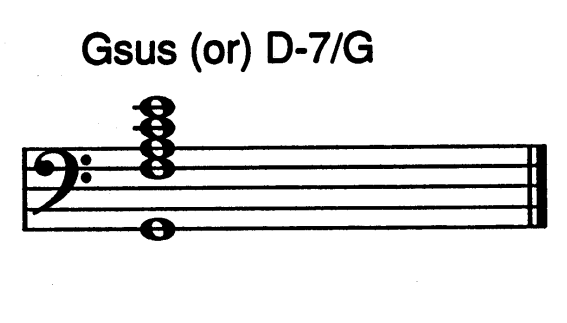
\includegraphics[width=2in]{levine_43.png}
	\label{Gsus}
\end{figure}

Levine's labels refer to (and within) two separate semiotic structures: $F/G$ is an interpretant produced by an agent (something analogous to a ``voicing algorithm" $A_1$ in Levine's brain) in response to voicing and pitch content, while a different agent (a ``function algorithm" $A_2$) uses nearly identical nomenclature ($D-7/G$) to index some property of the chord's function.\footnote{I mean this analogy to ground the semiotic processes involved in producing labels -- not as some cognitive description of Levine or any other analyst.  As Chapter 5 explains, the utter simplicity of algorithmic agents lends itself unusually well to explicit semiotic framings.}  Levine explains this function in strictly pitch-based terms -- ``your right hand plays a common $D-7$ left-hand voicing... over a $G$ root," and ``the $II-V$ progression in the key of $C$ is $D-7$, $G7$" -- but the functional interpretant is \emph{not} produced simply by analyzing intervallic voicing and pitch structure.\footnote{\cite{levine1989}, p.\ 23.}  Rather, Levine's presentation relies on a functional ontology in which $ii$ minor seventh chords have a property of leading to $V$ dominant sevenths in tonally syntactic progressions.   Despite the student analyst's observation that this sonority consists exclusively of pitch classes belonging to $F^9$, the voicing and progression behavior of $[0,10,14,17,21]$ leads Levine to produce $D-7/G$ as a functional interpretant.  

In a way, this sus-usage of $[0,4,7,11]$ remains true to the ethos of Levine's left-hand voicings.  Table~\ref{a_ii_lhv} assessed how frequently the LHV appeared as the upper voices of a minor seventh chord (typically preceding a dominant $V$, for Levine), but my interpretation of one of its statistics implied that the voicing also frequently appears as the upper voices of a sus chord (typically preceding or replacing $V$, for Levine).  In both cases, Levine carefully assigns a root to the chord, and in both cases the root is determined not by pitch content but by the typical behavior of the chord in tonal progressions.  This appeal to participation in certain kinds of syntactic progressions as a basis for the assignment of harmonic kinds will provide the basis for Chapters 3 and 4.

Figure~\ref{a_V_lhv} provides a simpler statistical portrait of the supersets for $[0,4,6,11]$, the left-hand A voicing Levine suggests for $V$.  Each of the ten most frequent appearances of a $[0,4,6,11]$ superset either (1) doubles a voice at the octave, (2) adds a chord extension appropriate to a dominant seventh with $[0,4,6,11]$ as its upper voices, or (3) adds the root required to turn $[0,4,6,11]$ into a fully-voiced dominant seventh (9,13) chord.  The superset data indicates that $[0,4,6,11]$ tends to appear in fewer contexts than $[0,4,7,11]$, both in terms of overall frequency and interpreted quality.  The voicing superset statistics for the B voicings, given here as Figure~\ref{b_ii_lhv} and \ref{b_V_lhv}, fit a similar narrative.  In each of these cases, the performance data indicates that Levine's left-hand voicings often appear as the upper voices of chords with the qualities he predicts.

\begin{table}%[h]
  \caption{Supersets of of Levine's $V$ ``A" left-hand voicing (LHV) $[0,4,6,11]$.}
  \centering
\begin{tabular}{l| l | l}
\hline\hline
Voicing & Counts & Potential interpretation \\ [0.5ex]
\hline
$[0,4,6,11]$ & 160 & LHV \\
$[0,4,6,11,18]$ & 31 & Voice 3 doubled \\
$[0,4,6,11,23]$ & 28 & Voice 4 doubled \\
$[0,2,4,6,11]$ & 23 & LHV + added root = dominant seventh (9,13) \\
$[0,4,6,11,16]$ & 22 & Voice 2 doubled \\
$[0,4,6,11,21]$ & 18 & LHV of $V$: added fifth \\
$[0,10,14,16,21]$ & 16 & LHV + added root = dominant seventh (9,13) \\
$[0,4,6,11,26]$ & 14 & LHV + added root = dominant seventh (9,13) \\
$[0,4,6,11,20]$ & 14 & LHV of $V$: added \# 11 \\
$[0,1,5,7,12]$ & 13 & Voice 1 doubled \\[1ex]
\hline
\end{tabular}
\label{a_V_lhv}
\end{table}

\begin{table}%[h]
  \caption{Supersets of of Levine's $ii$ ``B" left-hand voicing (LHV) $[0,4,5,9]$.}
  \centering
\begin{tabular}{l| l | l}
\hline\hline
Voicing & Counts & Potential interpretation \\ [0.5ex]
\hline
$[0,4,5,9]$ & 476 & Major seventh or $ii$ LHV \\
$[0,4,5,9,16]$ & 124 & Voice 2 doubled \\
$[0,4,5,9,19]$ & 107 & $ii$ LHV: added 11 or M7 add 9 \\
$[0,4,5,9,21]$ & 87 & Voice 4 doubled \\
$[0,4,5,9,17]$ & 69 & Voice 3 doubled \\
$[0,4,5,9,28]$ & 67 & Voice 2 doubled \\
$[0,7,11,12,16]$ & 65 & Voice 3 doubled \\
$[0,10,14,15,19]$ & 65 & $ii$ LHV: added root \\[1ex]
\hline
\end{tabular}
\label{b_ii_lhv}
\end{table}

\begin{table}%[h]
  \caption{Supersets of of Levine's $V$ ``B" left-hand voicing (LHV) $[0,5,6,10]$.}
  \centering
\begin{tabular}{l| l | l}
\hline\hline
Voicing & Counts & Potential interpretation \\ [0.5ex]
\hline
$[0,5,6,10]$ & 62 & $V$ LHV \\
$[0,5,6,10,20]$ & 17 & LHV + added root = dominant seventh \\
$[0,6,11,12,16,20,23]$ & 15 & Voice 3 doubled; if $V$ LHV: added \# 11, 13 \\
$[0,5,6,10,18]$ & 10 & Voice 3 doubled \\
$[0,5,6,10,17]$ & 10 & Voice 2 doubled \\
$[0,5,6,10,29]$ & 10 & Voice 2 doubled \\
$[0,5,6,10,27]$ & 8 & $V$ LHV: added fifth \\[1ex]
\hline
\end{tabular}
\label{b_V_lhv}
\end{table}

To assess the functional behavior of these chords -- whether they \emph{behave like} a $ii$ or $V$, instead of merely resembling one -- requires (more) engagement with keys and temporality.  A maximally transparent form of functional data mining would restrict itself to evidence like that given in Figure~\ref{[0,4,10,17]}, which implied local dominant-tonic relations directly from temporal voicing data and without the need to impose judgments regarding key.  But the claims of  Figure~\ref{[0,4,10,17]} are based on extremely slim data -- a handful of observations for each transition.  The pianists recorded in YJaMP use such a wide variety of voicings that tracking the progression behavior of each one individually would require a far larger corpus.\footnote{If the number of distinct voicings employed scales roughly linearly with the number of pianist-hours recorded, no corpus of any size could produce the relevant statistics.  I assume, however, that the number of distinct voicings will level off much faster than the number of recordable performances, rendering the problem accessible at large scale.}  As Levine already implies by describing ``voicings" in terms of their progression behavior relative to local key centers, transposing the wide variety of possible voicings relative to their local keys greatly reduces the size of the computational alphabet -- and generates a new ontological framing amenable to syntax.

\section{Scale degrees and key finding}

Since many corpus analysts view their computational tasks as attempts to replicate the cognitive properties of a human listener or analyst, the algorithmic assignment of keys to passages of music sits at the heart of a wide variety of otherwise disparate harmonic analysis projects.  Starting at least as early as the (human) experimental work of Krumhansl, Schmuckler, and Kessler of the 1980s, keyfinding studies typically assume that key determinations arise at least partly in response to pitch-class distributional patterns.\footnote{See \cite{krumhansl1982} and \cite{krumhansl1990}.}  Whether generated by probe-tone studies of perceived stability or key-appropriateness for particular chords and pitch classes (Krumhansl 1990), melodic pitch class statistics from the Essen folk music corpus (Aarden 2003), or polyphonic pitch class frequencies from 18th and 19th-century art music (Aarden 2003, Bellmann 2005, Temperley 2007), key profiles generally assume the form of a twelve-dimensional probability distribution indicating the likelihood or prevalence of each pitch class given a particular key.\footnote{See \cite{krumhansl1990}; \cite{aarden2003}; \cite{bellmann2005}; \cite{temperley2007}, Ch. 6.  Automated key-finding based on statistics other than pitch class distributions can also yield excellent results, as in \cite{quinn2010}, but this study constitutes a significant outlier in the literature.} The specific parameters vary from profile to profile, but the general results for western tonal repertoires tend to resemble Figure~\ref{krumhansl} (reprinted from \cite{krumhansl1990}), whether arising from perception studies or corpus statistics.

\begin{figure}%[h]
	\centering
	\caption{Figure 3.3 from \cite{krumhansl1990}.  The relative frequencies for each pitch class relative to the local tonic (given as $C$, on the horizontal axis) for several small corpora (circles, triangles, and squares) and human perception studies (diamonds).}
	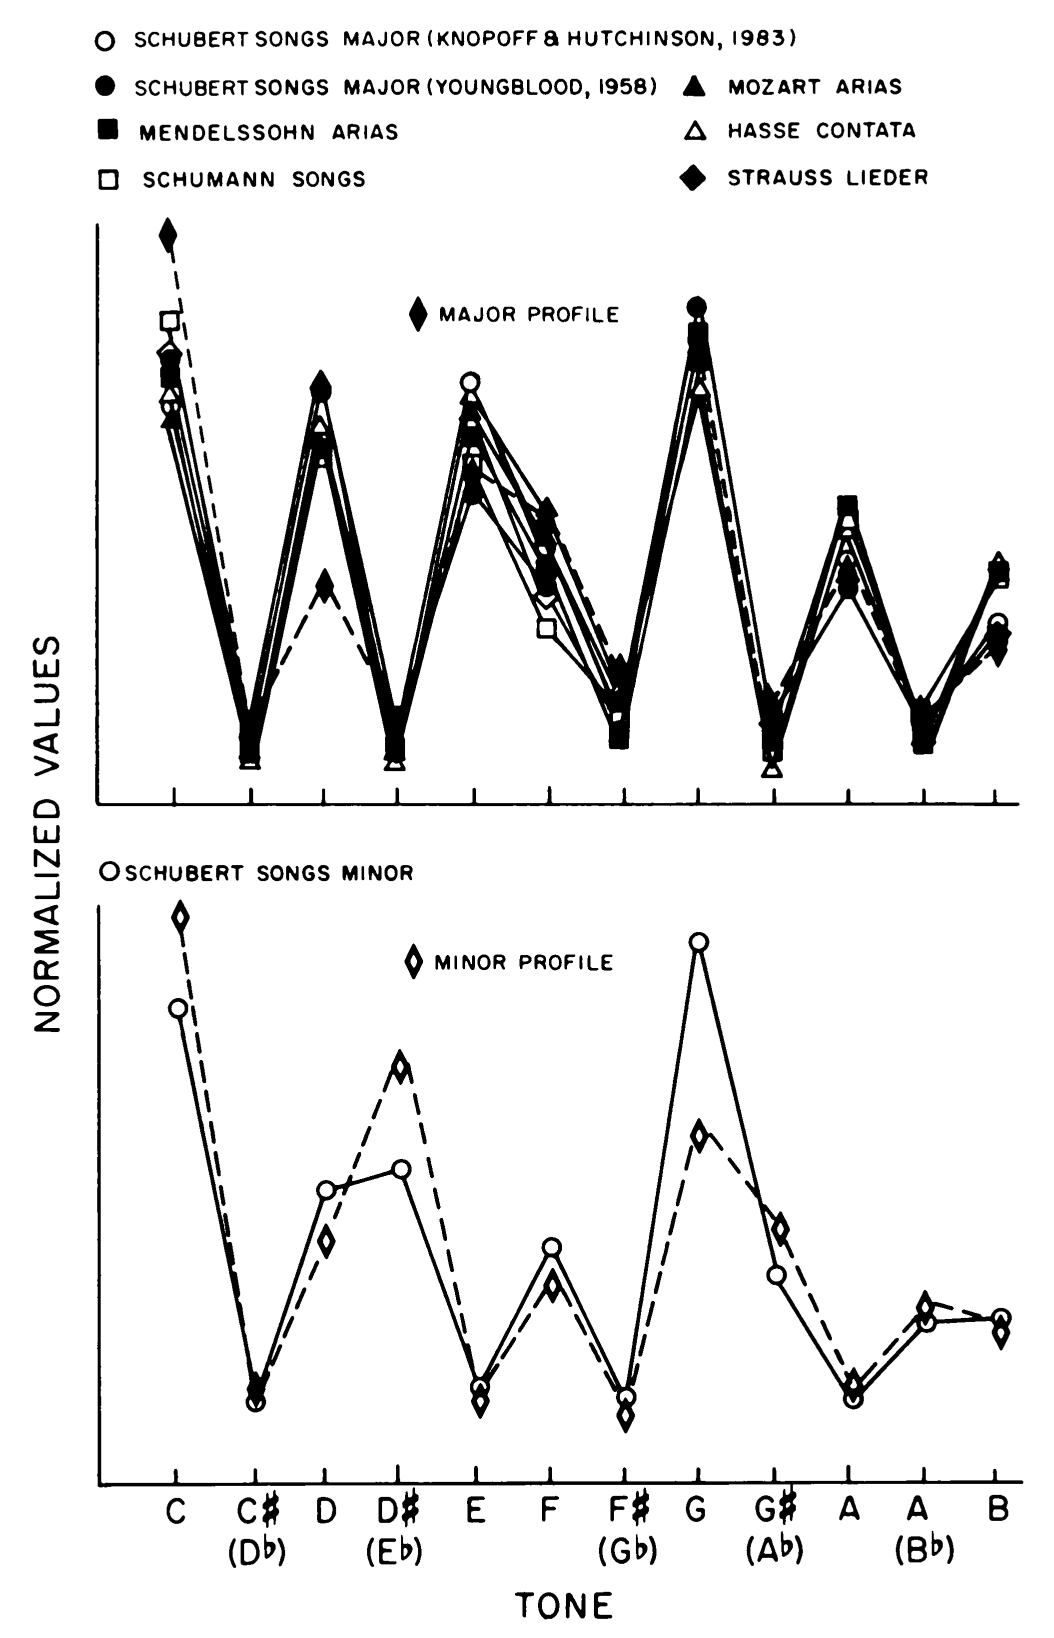
\includegraphics[width=4in]{krumhansl.png}
	\label{krumhansl}
\end{figure}

Figure~\ref{krumhansl} presents similarly-shaped profiles generated in distinct ways.  The diamond-dotted ``major" and ``minor" profiles plot a stability or goodness-of-fit rating listeners assigned each pitch class when played in the context of the relevant key.  A higher vertical axis value for these curves indicates that the experimental subjects considered the pitch class very stable or appropriate to the key, while lower values indicate the opposite.  The curves delineated by circular, triangular, or square dots plot a normalized measure of frequency of appearance for each of these pitch classes in key-analyzed corpora from different composers.  The absolute scale is unimportant -- the major contribution of Figure~\ref{krumhansl} is to indicate the relative importance of each scale degree to a local key and to show a close fit between profiles generated from perception studies and those generated from pitch class statistics.\footnote{For further experimental details, see \cite{krumhansl1982}; for wider context, see \cite{krumhansl1990}.}

Armed with these (or similar subsequent) major and minor key profiles, key-finders typically tally the pitch class distributions for a given musical passage and use some basic quantitative methods to select which assumed tonic's profile would produce the best fit.  Any key-finding algorithm written along these lines needs three essential inputs:
\begin{enumerate}
	\item A selected passage for which the key is desired but not known
	\item A set of theoretical key profiles
	\item A goodness-of-fit measure by which the statistics from (1) can be compared to (2)
\end{enumerate}
%first: the perpexity-based segmentation process
These inputs correlate to a segmentation problem, a parameterization problem, and an optimization problem, respectively.  While some studies approach segmentation (1) with broad heuristics, like using the pitches of an entire piece\footnote{\cite{krumhansl1990} or the first and last 8 measures of each piece\footnote{\cite{albrecht2013}}, others chop each piece into many parts and assign a probable key to each.\footnote{See \cite{temperley2007}; \cite{white2013}.}  As Temperley notes, segmenting a piece into many consecutive ``windows" allows a key-finding model the flexibility to identify modulations.\footnote{\cite{temperley1999}, pp.\ 78-81.}  But while Temperley makes a convincing case for the necessity of windowed segmentation in key finding, he provides no real heuristic for the determination of window size.\footnote{See \cite{temperley1999}, p.\ 81, for example, where ``Segments of about 1 measure -- typically between 1 and 2 s long -- proved to be about optimal..."  This heuristic carries over to \cite{temperley2007}.}  Most windowed key-finding algorithms choose a set number of measures, beats, or note onsets as an appropriate window, despite Temperley's caveat that ``[t]his also means that the tempi chosen for pieces may affect the program's analysis."\footnote{\cite{temperley1999}, and see also the eight quarter-note window employed in \cite{wq2017}.  Sliding these fixed windows through the corpus with an incrementing interval of a quarter note allows White and Quinn to determine modulations over durations shorter than eight quarters.}

Setting a window size by measures or beats runs the risk of attempting key assignments for segments of radically different cardinality.  Fortunately, a performance corpus like YJaMP affords the examination of timing data taken directly from note onsets, bypassing notational questions regarding measure lines, beats, or notated tempi.    Figure~\ref{cardinalities} displays the output of a simple counting algorithm;\footnote{This windowing code and other key-finding methods discussed here are available at \href{github.com/andrewdjones/YJaMP_Analysis}{github.com/andrewdjones/YJaMP\_Analysis}.} for temporal window sizes of 400ms, 800ms, 1.6s, and 3.2s, the algorithm tallies the number of windows with each pitch-class cardinality corpus wide.  On average, 400ms windows tend to capture pitch-class sets of cardinality 3-5, the smallest cardinalities at which we might expect to find traditional chord objects carrying harmonic information, while windows of longer duration gradually increase in average cardinality.  Windows of 1.6 seconds tend to contain about 7 pitch classes -- the start of what we might call the scalar regime -- and 3.2 second windows begin to approach the 12-tone aggregate.

The smooth logic of these curves hides reasons for the key-finder to worry.  If the corpus is segmented into 400ms segments, some of them will contain only two pitch classes -- likely too few for any meaningful key assignment -- while others contain seven or eight.  Algorithms segmenting windows based on a particular number of note onsets might seem to solve the problem, but they prove highly sensitive to repetitions and decorative figurations.\footnote{For an example of repetition-sensitivity for small windows, see Chapter 6 of \cite{temperley2007}.  While Temperley advocates ignoring repetitions to mitigate the problem, I retain this information and adjust the window sizes accordingly.}

To account for both disparities, I employ a key-finding algorithm with a variable window size set through distributional means.  Collections of pitches well-suited to key-finding will contain an instance or two of several pitch classes, consisting neither of one pitch class (potentially repeated many times) nor the undifferentiated aggregate.  If all twelve pitch-classes appear, they should appear with different relative frequencies, or else the key-finder will make a pseudo-random choice.  Rather than requiring a particular number of notes per window, my key-finding algorithm calculates the average perplexity of segmented pitch-class distributions for a range of possible window sizes for each tune; it then selects whatever window size results in an average perplexity closest to that of the key profiles.

%cardinality at time scale stats (could be remade to look better)
\begin{landscape}
\begin{figure}
	\centering
	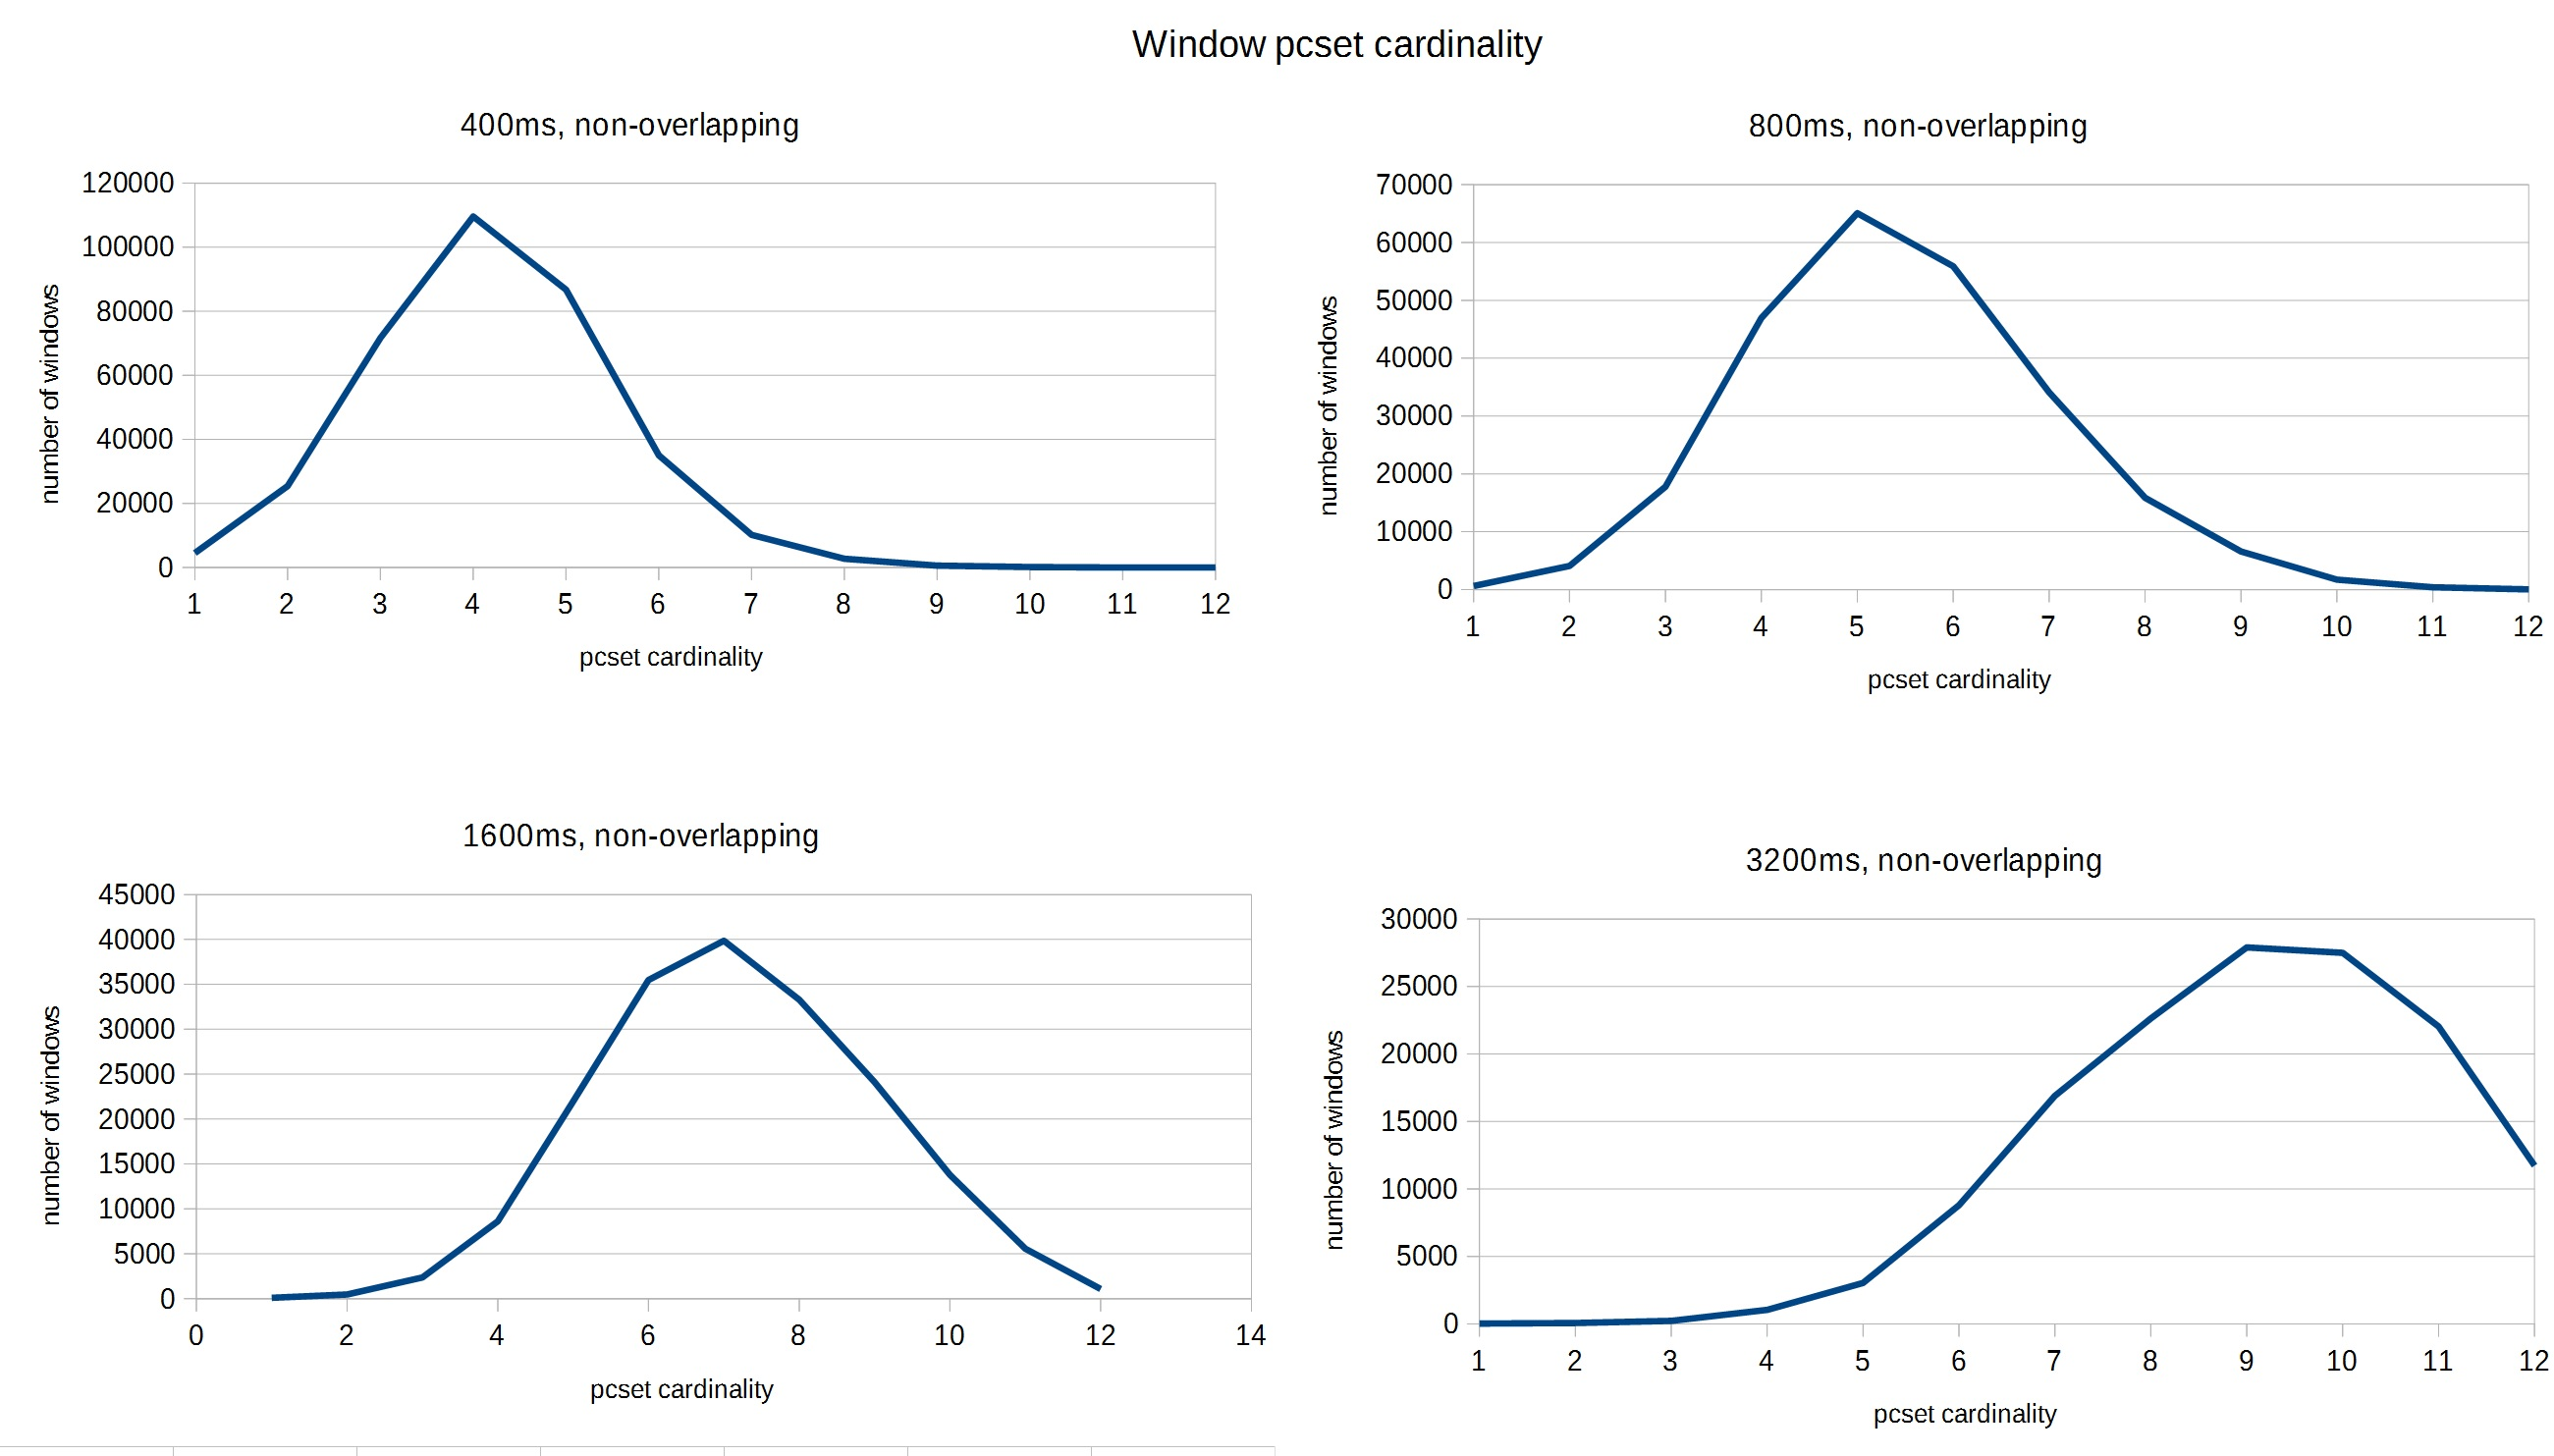
\includegraphics[width=8in]{cardinalities.jpg}
	\caption{Average pc-set cardinalities for four window sizes.  As window size increases, so does average cardinality.}
	\label{cardinalities}
\end{figure}
\end{landscape}

%perplexity and entropy
Perplexity, alongside its information-theoretical partner entropy, can be used to provide a measure of the diversity or disorder of a probability distribution.  A perfectly flat pitch class distribution, which would resemble a horizontal line on Figure~\ref{krumhansl}, corresponds to a high perplexity, where each of the twelve pitch classes would be equally likely to appear -- if asked to guess the pitch class of a particular note in the passage, the distribution would do a pretty (in fact, maximally) poor job.  The distribution for a passage consisting of a single pitch class would have a very low perplexity, indicating that the distribution could predict a particular note in the passage with extremely high certainty; if the passage's pitch-class distribution consisted of $100 \%$ $C$ and $0 \%$ for every other pitch class, it would be maximally ordered and perfectly predictive over the passage.

Key profiles like the Krumhansl-Schmuckler, Aarden-Essen, Temperley-Kostka-Payne, or Bellman-Budge resemble neither case.  These distributions encode information regarding the relative importance of different pitch classes, so their pitch ``guesses" will not be completely random, as they would be in the flat-distribution, high-perplexity case.  But each of these key profiles also encodes non-zero probabilities for all twelve pitch classes, acknowledging that the determination of a passage's key does not preclude the appearance of any member of the aggregate.  Key profiles imply that the pitch-class distributions of tonal music are partially ordered and partially disordered -- not in music theoretical senses of higher/lower pitch, syntax, or voice leading, but in the sense that tonal passages typically contain pitch classes appearing in unequal relative proportions predictable in advance.

The perplexity $PP$ of a probability distribution $p$ may be calculated from its entropy $H(p)$:
\begin{equation}
PP = 2^{H(p)} = 2^{-\sum_{x} p(x) \log_2 p(x)}
\end{equation}
The summation here takes each possible value $x$ (in the pitch-class case, there are 12) and adds up the sum of the value's probability $p(x)$ times the logarithm of its probability $\log_2 p(x)$.  In the flat-distributional case where each of the 12 pitch classes is equally likely, this reduces to the maximum perplexity of a key profile:
\begin{align*}
PP &= 2^{-\big(\frac{1}{12} \log_2 \frac{1}{12} + \frac{1}{12} \log_2 \frac{1}{12} + ...\big)} \\
 &= 2^{-12\big(\frac{1}{12} \log_2 \frac{1}{12}\big)} \\
 &= 2^{-\log_2 \frac{1}{12}} = 2^{\log_2 12} = 12
\end{align*}
Heuristically, perplexity tells us that the model is like the roll of a $PP$-sided die; in the flat-distributional case, predicting a single pitch would be literally equivalent to rolling a fair 12-sided die.  At the other extreme, a minimally-perplexed probability distribution containing a single pitch class with $100\%$ probability has a perplexity of 1 -- its predictions are like rolling a single-sided die.

To match a given passage's pitch-class probability distribution perplexity to that of a key profile, I note that the Bellman-Budge profile yields a perplexity of approximately 8.1 -- similar to that of rolling an 8-sided die.\footnote{Other profiles yield very similar perplexities.  For example, I generated pitch-class profiles for each tune head in the corpus, assembling statistics based on hand-annotated keys in order to produce a ``YJaMP key profile."  The resulting vector hewed fairly closely to Bellmann-Budge (\cite{bellmann2005}), both in terms of its perplexity and the distribution's overall shape.  For code details, see jazzKey.py at \href{github.com/andrewdjones/YJaMP_Analysis}{github.com/andrewdjones/YJaMP\_Analysis}.}  Whichever segmentation window size produces probability distributions with perplexities closest to that value is likely the most appropriate for each recording.  The duration of these windows ranges from a couple of seconds in fast tunes to 30 seconds or more in ballads.

%sliding and cosine optimization
Optimizing the resulting choice of key for each window proceeds in two steps.  First, the key-finding algorithm segments a window of the perplexity-calculated duration and compares its pitch-class distribution to the Bellman-Budge profiles.  I assume that key-to-key variance in profiles is small, so the algorithm sees the same major mode profile and minor mode profile for each possible tonic.  It then choose whichever Bellman-Budge transposition minimizes the cosine distance between it and the window's distribution.  The cosine distance measures the directional alignment of the two twelve-dimensional vectors, discounting their magnitude; this encodes the notion that the absolute frequencies of appearance for pitch classes in the window and profile matter less than their proportional relation to one another.\footnote{Formally, the cosine distance $\cos(\theta)$ between two pitch class vectors $\mathbf{p_1}$ and $\mathbf{p_2}$ is $\cos(\theta) = \frac{\mathbf{p_1} \cdot \mathbf{p_2}}{\| \mathbf{p_1} \| \| \mathbf{p_2} \|}$, the dot product of the vectors divided by the product of their magnitudes.  This approach is similar to but distinct from the Euclidean metric advocated in \cite{albrecht2013}.}  Second, following \cite{wq2017}, the key-finder slides the window through the composition by a small durational increment and re-calculates the best-fit key at each step.

%Sliding, interonsets, and chord temporal stability
Setting this sliding increment impacts both the rate at which the algorithm produces key changes and, more subtly, the ontology in which chords are embedded.  Generally speaking, key assignments change as new pitch classes modify the locally-windowed distribution, and the window sliding increment represents the shortest possible time scale over which the algorithmic agent looks for such changes.  But short-duration, absolute time sliding increments also challenge the temporal stability of chord objects, since the limiting case (say, an increment of 1ms) might well separate pitches we (or an algorithm) might otherwise count as part of the same ``chord" into several different windows.  As a consequence of YJaMP's MIDI encoding, the temporal quantization performed by printed scores never aligns near-simultaneities into exact verticalities -- so the choice of what to call a ``chord" must be made on temporal and distributional grounds.

%Describe inter-onset plot
Figure~\ref{io_plot} plots inter-onset times between the individual pitches of the YJaMP corpus.  Taken directly from the MIDI onset times for each piano key struck, this plot displays how many note-to-note inter-onsets appear in the corpus for a range of possible times stretching from 0ms up to 500ms.  Toward the far right of the figure, an inter-onset time of 450ms indicates a comparatively long gap between two key strikes, while inter-onsets toward the left of the figure indicate nearly simultaneous strikes.  Since the MIDI piano setup loses accuracy below about 5ms, the erratic behavior of the plotted distribution between 0-10ms should be taken with a grain of salt.  At spans above 10ms, however, a relatively smooth distribution emerges, where a very large number of inter-onsets at short times decreases rapidly to a local minimum around 50-60ms.  At durations longer than this scale, the number of inter-onsets displays a slight increase; it only returns to the 50-60ms local minimum around 200ms, after which the long tail tapers off.

I note that this distribution intuitively matches what we might expect from superimposing two separate distributions -- one chi-squared like (for $k=1$), with a maximum at $t=0$ms, and one normal or Gaussian-like, with a mean around $t=130$ms.  The populations represented by the two distributions might then map onto the temporal behavior expected of intra-chord inter-onsets, like fast melodic runs or pitches rolled but struck nearly simultaneously, and inter-chord onsets, as when one roughly simultaneous chord sounds some temporal delay after another.  To posit Figure~\ref{io_plot} as arising from the statistics of two different populations is to enunciate an ontological framing for chords: under such a description, chords consist of sets of pitches struck very close to one another (that is, within about 50ms) which tend to be separated from one another by 50-200ms.  Chords might be thought to ``stabilize," temporally speaking, around 50ms.\footnote{Empiricists and interpreters alike tend to locate the shortest span for human auditory attention in this regime; Justin London and Michel Chion cite 100ms and 40ms, respectively. (\cite{london2012}, p.\ 28; \cite{chion2016}, p.\ 24.)  Note that neither kind of analyst does so on the basis described here.}  As a result, the shortest-duration objects the algorithms of Chapters 3 and 4 tally as ``chords" are the contents of 50ms time windows.

\begin{figure}
	\centering
	\caption{A plot of note inter-onsets versus time for pitches in the YJaMP corpus.  Two types of behavior appear: decreasing counts as time increases, for very short times, and increased counts between 50ms and 200ms.  Below about 5ms, the MIDI piano's accuracy becomes erratic and suspect.}
	\label{io_plot}
	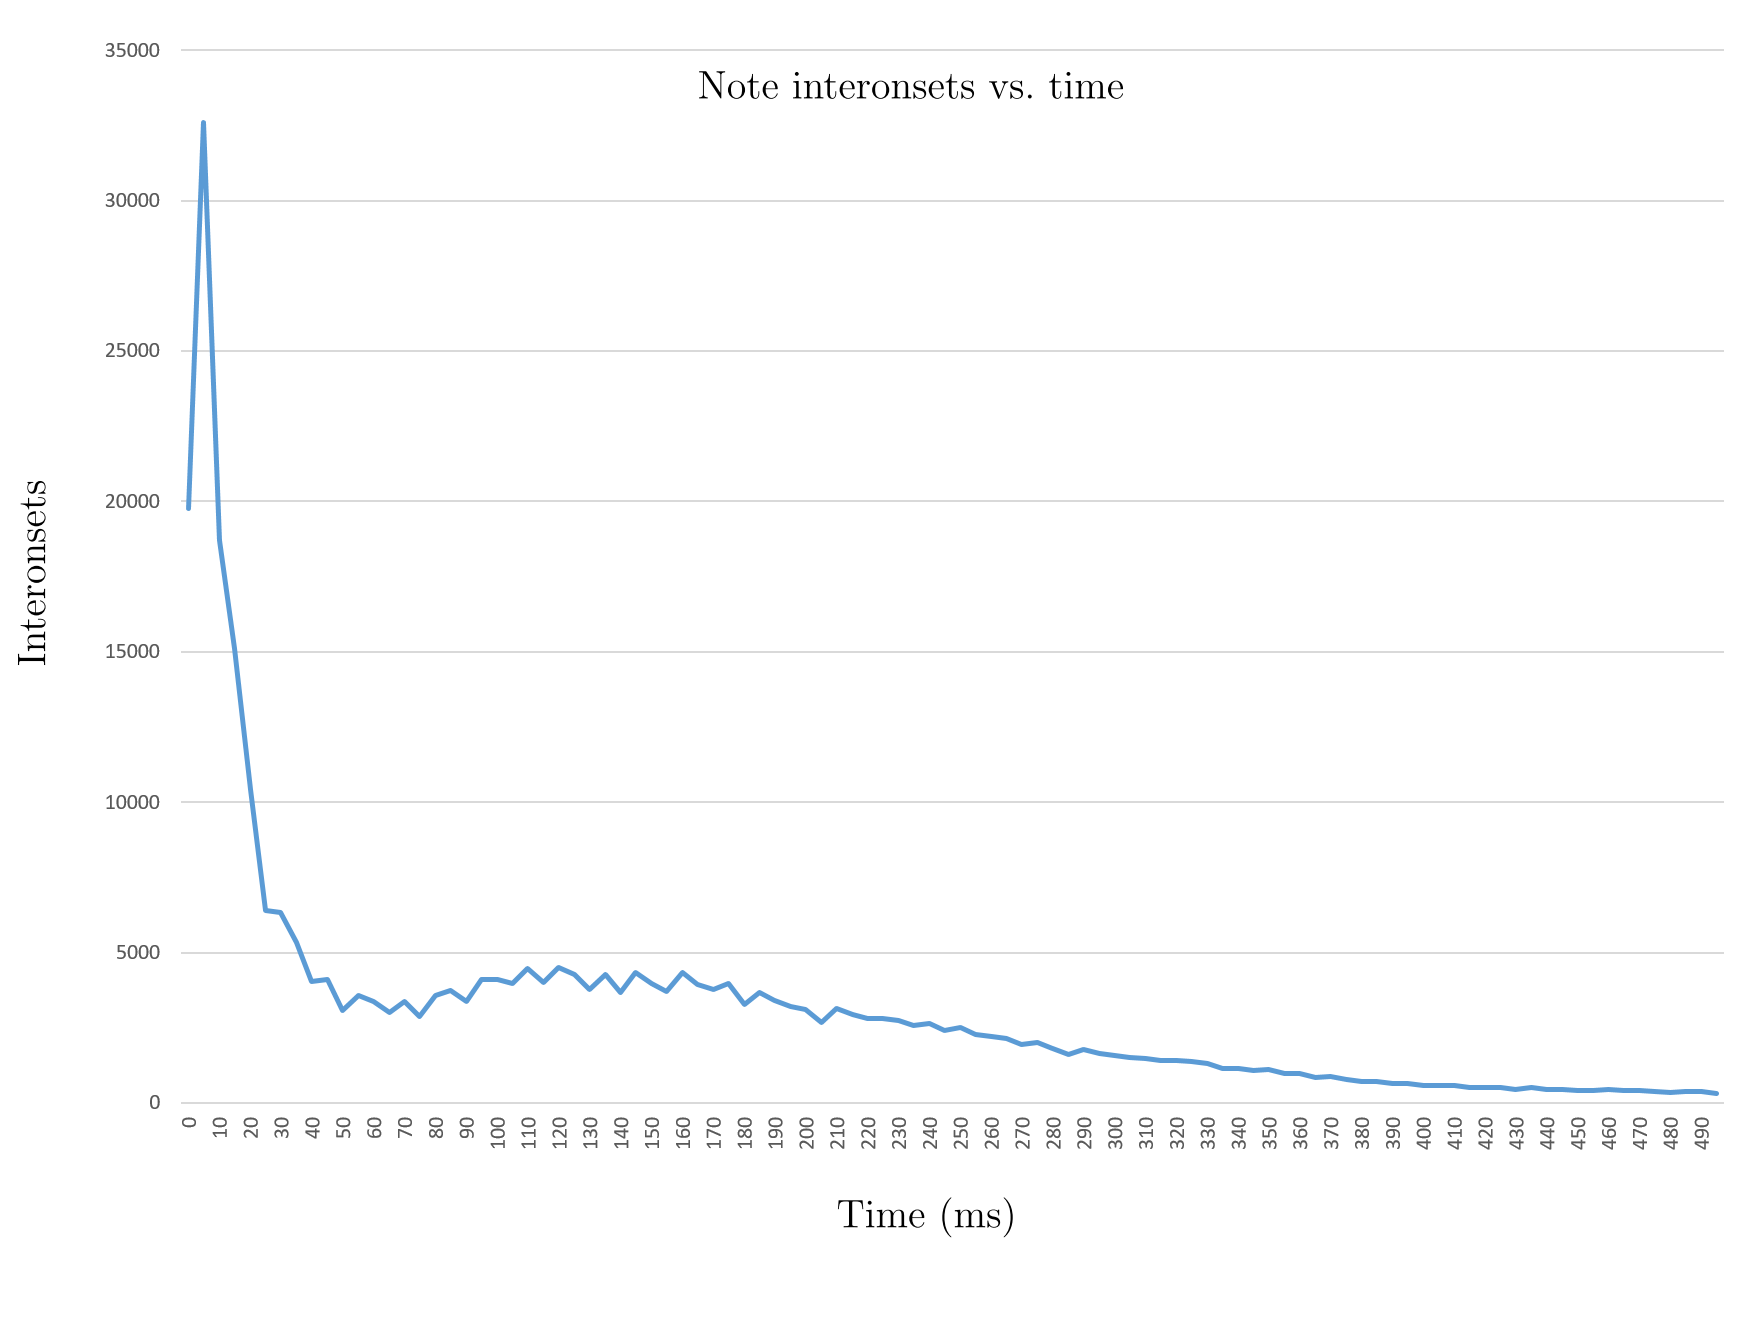
\includegraphics[width=5.9in]{io_plot.png}
\end{figure}

%sliding increment from perplexity change
The status of the 50ms inter-onsets also has ramifications for window perplexity. At very short window sizes (below 50ms), the average perplexity across all windows in a given performance levels out at approximately the average number of pitches sounding at any given moment.  For each recorded track, there is then some slightly larger window size at which the average perplexity begins to increase over this baseline level.  The time scale at which average window perplexity first increases by $30\%$ over its short-duration (ca.\ 50ms) value sets the sliding increment for the segmented windows in the key-finding algorithm.  We might think of this sliding increment, which varies from track to track, as the shortest time scale at which chords might be expected to change at the track's performance tempo. 

%confidence
As a result, each ``chord" in a tune ends up in several possible windows of the same duration.  Since the key-finding algorithm assigns a best-fit key for each window, each chord may have several different possible key assignments.  To disambiguate, the algorithm employs a confidence measure: the degree to which a given key assignment outperforms the model's next-best guess.  Since the predicted key for a window corresponds to the minimum cosine distance ($d_1$) between the window's distribution and the possible key profiles, the model's next-best guess is the key with the second-shortest distance ($d_2$).  One measure for the confidence of the model's guess is then $1 - d_1/d_2$, which approaches 1 when the best guess is very close to the window distribution and the second-best is very far.  If no windows containing a particular chord have confidences higher than $30\%$, I mark the key as ambiguous; otherwise, the key-finder tags the chord with the local key from the window yielding the highest confidence value.

%problematize/ontologize
It is worth asking whether this ``key" assignment really says the same thing as a human-annotated one.  ``Key" in general stands for a complex concept entangling macroharmony and centricity, to borrow Tymozcko's formulation regarding limited pitch class collections with some tonic.\footnote{See \cite{tymoczko2010}, especially Chapters 1 and 5.}  Human listeners or analysts presumably consider voicing, cadence and phrase structure, metric placement, and many other factors when determining a passage's key.  Key-finding algorithms based on pitch-class profiles, however, employ algorithmic agents instead of human ones, and the properties of the resulting key determinations are grounded only in the indexical signs the algorithm uses to make its decisions.  When an algorithmic key-finder of this kind $A_1$ and a human agent $A_2$ both determine that a passage of music ``is in" a particular key, the interpretants refer to objects ($O_1$, $O_2$) with necessarily different semiotic ontologies.  For the algorithm, keys do not have properties like ``indicated by many $ii-V-I$ progressions" or ``signaled by passages ending with a cadence in the tonic" (though pitch-class translation of the former might find indirect support in the passage's pitch class statistics).

I do not claim that each key assigned to a passage by the algorithm corresponds to the kind of key object a human would assign, but rather that the automated key assignments afford certain kinds of indexical inquiry.  If a human analyst assigns a key to a passage by noticing what appears to be a $V-I$ progression, the resulting representation of the data already encodes chord-behavioral assumptions grounded in the way the agent turns signed indices into key interpretants.  This is excellent for the accuracy of key identification, but it introduces potential circularity if the analyst then tries to determine what harmonic progressions occurred in the passage.  When an analyst states that $V-I$ has an important progression status in any given key, the claim reflects both the properties of the key category and the response to indices by which it is observed and assigned.  If an algorithmic agent of the kind above can be made to say that $V-I$ has an important progression status in any given key, the claim rests on a different semiotic structure -- with no \emph{a priori} knowledge about what kinds of progression index a key, key profile-tagged corpora can provide an important ground for claims regarding tonal syntactic progressions.

%set up transposition to scale degree sets
With these keys in hand, chapters 3 and 4 pursue inquiry of this type.  To isolate syntactic progressions relative to some local key, the key-finding algorithm assigns keys to each chord in the music and converts all pitch-class sets into local, chromatic \emph{scale-degree sets}.  Each scale-degree set consists of the semitonal pitch-class set data transposed relative to the local key.  Relative to the local tonic (set as chromatic scale degree 0), Table~\ref{sds} shows the most frequent scale-degree sets of cardinality 4 or greater found in YJaMP.

\begin{table}
\caption{The most common locally-transposed scale-degree sets in the YJaMP corpus with cardinalities larger than 3.}
  \centering
\begin{tabular}{l | l | l}
\hline\hline
Scale-degree set & Counts & Potential interpretation \\ [0.5ex]
\hline
$[0, 4, 7, 11]$ &	2783	& $I^7$ \\
$[0, 4, 5, 9]$ &	2217	& $IV^7$\\
$[2, 4, 7, 11]$ &	2110	& $iii^7$\\
$[0, 2, 4, 7]$ &	1924	&\\
$[0, 2, 5, 7]$ &	1878	&\\
$[0, 3, 7, 8]$ &	1804	& $\flat VI^7$\\
$[0, 4, 7, 9]$ &	1712	& $vi^7$\\
$[0, 2, 5, 9]$ &	1659	& $ii^7$\\
$[0, 5, 7, 9]$ &	1253	&\\
$[0, 3, 5, 7]$ &	1252	&\\
$[0, 2, 7, 9]$ &	1238	&\\
$[0, 2, 4, 7, 11]$ &	1165 &	$I^9$\\
$[0, 2, 7, 8]$ &	1128	&\\
$[0, 2, 7, 11]$ &	1114	&\\
$[2, 5, 7, 11]$ &	1105	& $V^7$\\
$[0, 4, 5, 7, 9]$ &	1093	& $IV^9$\\
$[2, 4, 7, 9]$ &	1055	&\\
$[2, 7, 9, 11]$ &	1009	& $V$ add \nth{9}\\[1ex]	 
\hline
\end{tabular}
\label{sds}
\end{table}

This seemingly-unremarkable list makes no assumptions about chord structure, consonance, or voice-leading.  Dissonant clusters are treated exactly the same as stacks of perfect fifths, pentatonic scales, and seventh chords.  No reduction of non-harmonic tones has been employed.  Nevertheless, scale-degree sets corresponding to $I^7$, the local tonic, constitute the most frequent four-note scale-degree sets in the corpus, and minor, major, and dominant seventh chords on scale degrees strongly predicted by traditional syntactic theories all appear high on the list.  As these chords were not known to the algorithmic agent making the key assignments, we might take their appearance here as confirmation that human analysts are right to connect chord progressions and keys.  Chapter 3 uses $ii$ chords to introduce methods for examining the temporal progression properties of scale-degree sets, and Chapter 4 provides methods for grouping scale-degree sets into categories based on similarities in their progression statistics.  Both of these modes of analysis rest on the particular nature of these scale-degree sets -- this particular method of turning the YJaMP recordings into harmonic objects.  Just as the first half of this chapter used algorithmically-produced voicing objects to both complicate and lend support to jazz theoretical interpretants, the following chapters will treat scale-degree set objects as signed indices in an attempt to reproduce and expand traditional statements regarding syntactic progressions.  Many object-ifications of a performance corpus are possible, but the one presented here affords a particular alignment between computational semiotic processes and human-analytical ones.
	
%Chapter 2, on objects, needs a LOT.  Consider Kockelman here, alongside extensive descripton of my key-finding and parsing methods?  (That has to go somewhere, and here seems like the only place)
\chapter{Progressions}

Figure~\ref{iiprog} presents one of the most common truisms circulated regarding jazz harmony in a new form.  Each of the curves plotted here describes the statistical behavior of a chord category following the appearance of a locally-transposed $ii$ chord.\footnote{For details regarding the key-finding and local transposition, see Chapter 2.}  The details of Figure~\ref{iiprog} will emerge below, but the general form of the plot is simple: the vertical axis gives a measure of probability, while the horizontal displays time elapsed after a $ii$ chord.  Each curve tracks the probability of a particular chord appearing after $ii$ over time.

\begin{figure}
	\centering
	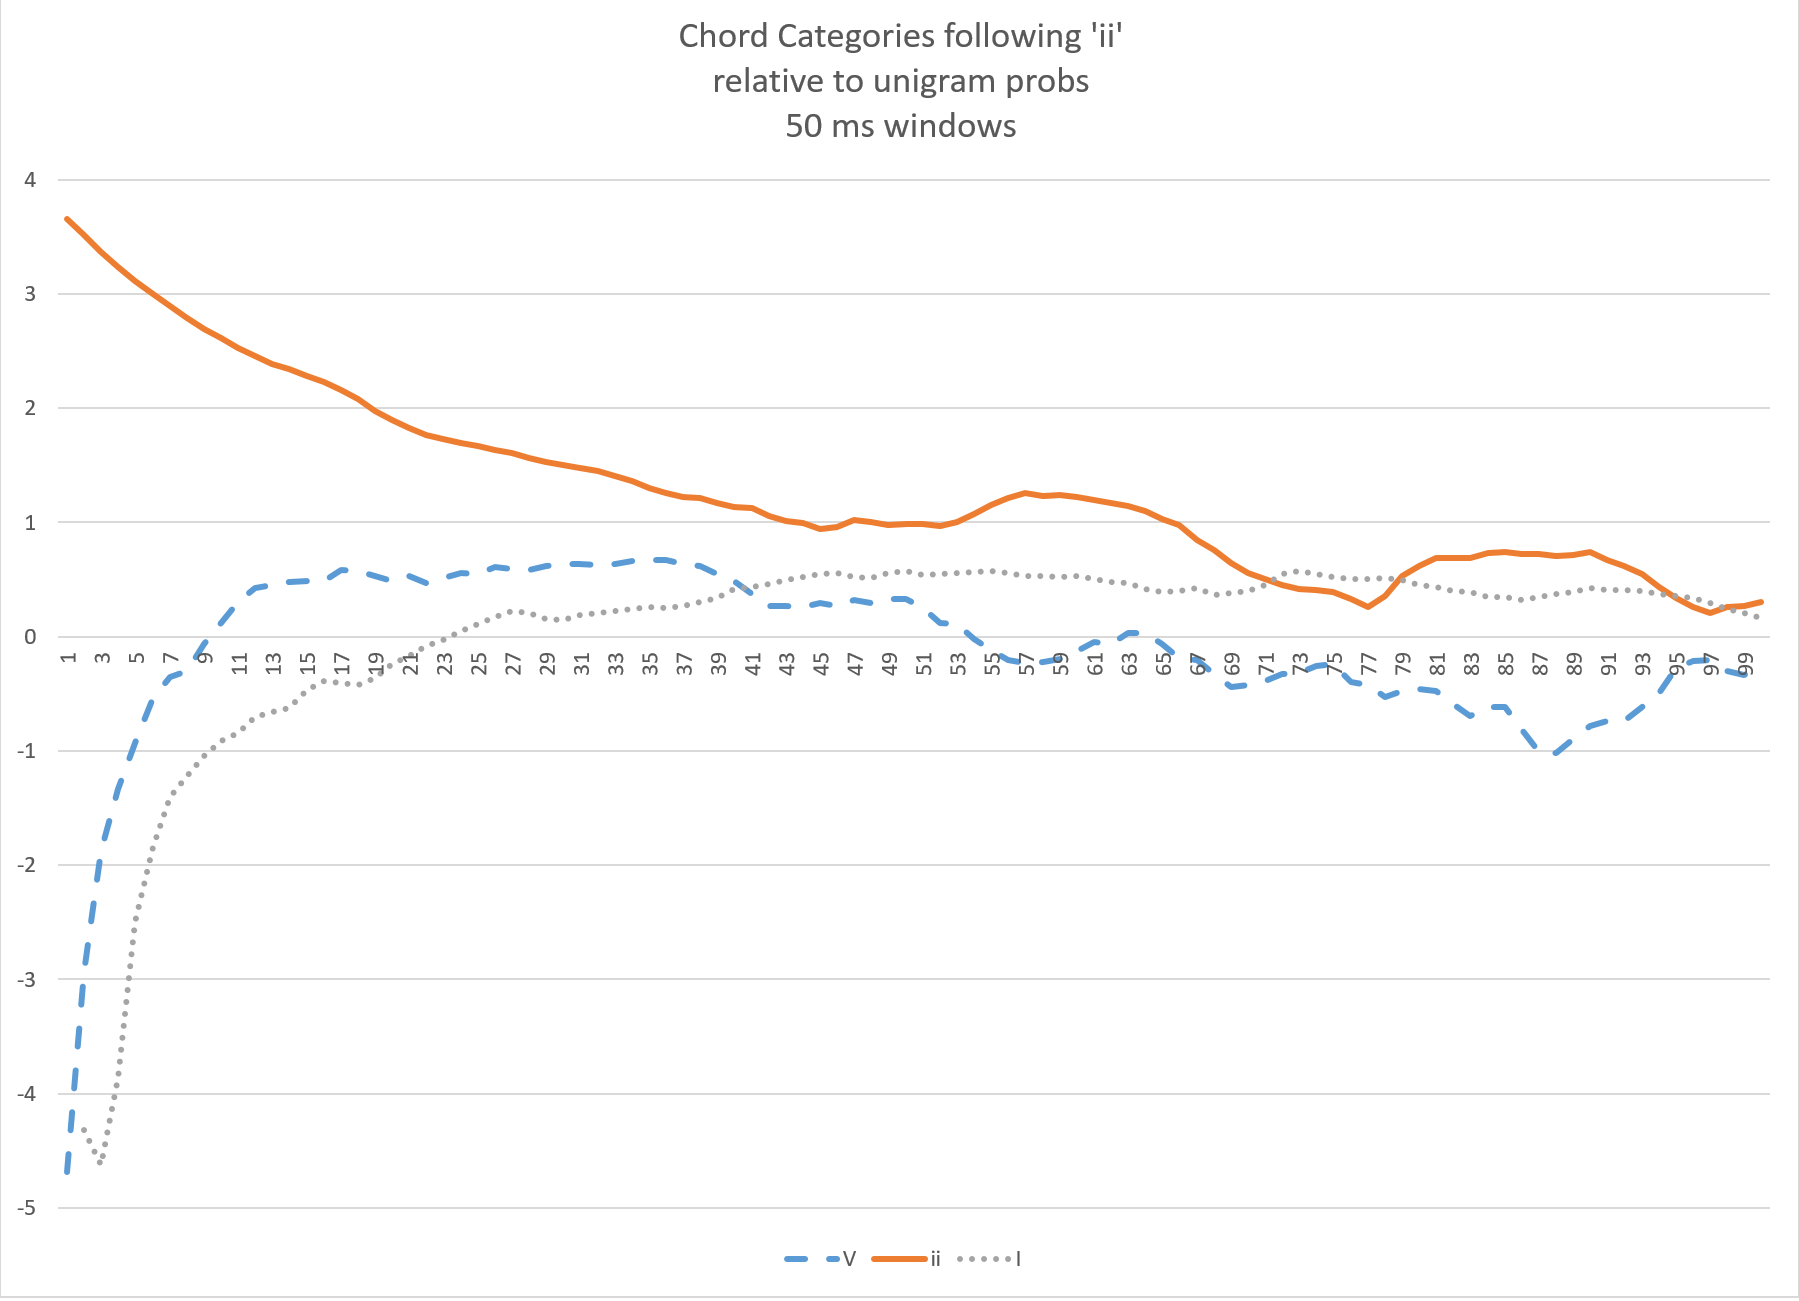
\includegraphics[width=5.8in]{iiprogressions.png}
	\caption{The unigram-relative log probabilities of $ii$ (blue, dashed line), $V$ (gray, dotted line), and $I$ (red line) versus time (in milliseconds) elapsed after a $ii$ chord in the YJaMP corpus.  Here, the categories for $V$, $ii$, and $I$ have been hand-chosen; Chapter 4 provides a means to bootstrap category formation.}
	\label{iiprog}
\end{figure}

The truism: in jazz, $ii$ often progresses to $V$ and then to $I$.  The curves of Figure~\ref{iiprog} have different shapes -- different behaviors over time -- which might be said to demonstrate and destabilize the truism in and with explicitly temporal terms.  The (gray, dotted) curve for $V$ rises to a probability peak between 500 and 2000 milliseconds, after which it slowly decreases in probability.  The (red, solid) curve for $I$ starts out less probable than $V$, but it becomes more probable as time elapses, surpassing $V$ around 2000ms.  Cast in traditional terms, these curves imply that when a $ii$ chord appears, it is likely that a $V$ chord appears some short time later, while a $I$ chord will probably appear some time after that.  This representation avoids bigram-style transitions between immediately adjacent states, instead displaying probabilistic tendencies over time.

The (blue, dashed) curve corresponding to $ii$ on Figure~\ref{iiprog} seems superfluous with respect to the truism above.  It shows that at very short times after the appearance of a $ii$ chord, another (or perhaps the same) $ii$ chord is highly probable.  When compared to the other curves on the plot, the $ii$ curve shows a very different shape and behavior.  I will return to this and the details of Figure~\ref{iiprog} in the following sections, but for now it suffices to note that this plot encapsulates at least two different scales of behavior: local reappearance of $ii$ and ``delayed" (however minimally) appearance of $V$ and $I$.  These modes of progression place it into dialog with schematic diagrams like Figure~\ref{pers}, taken from the harmonic progression work of Christopher Wm. White and Ian Quinn.\footnote{See \cite{wq2017}.}

\begin{figure}
	\centering
	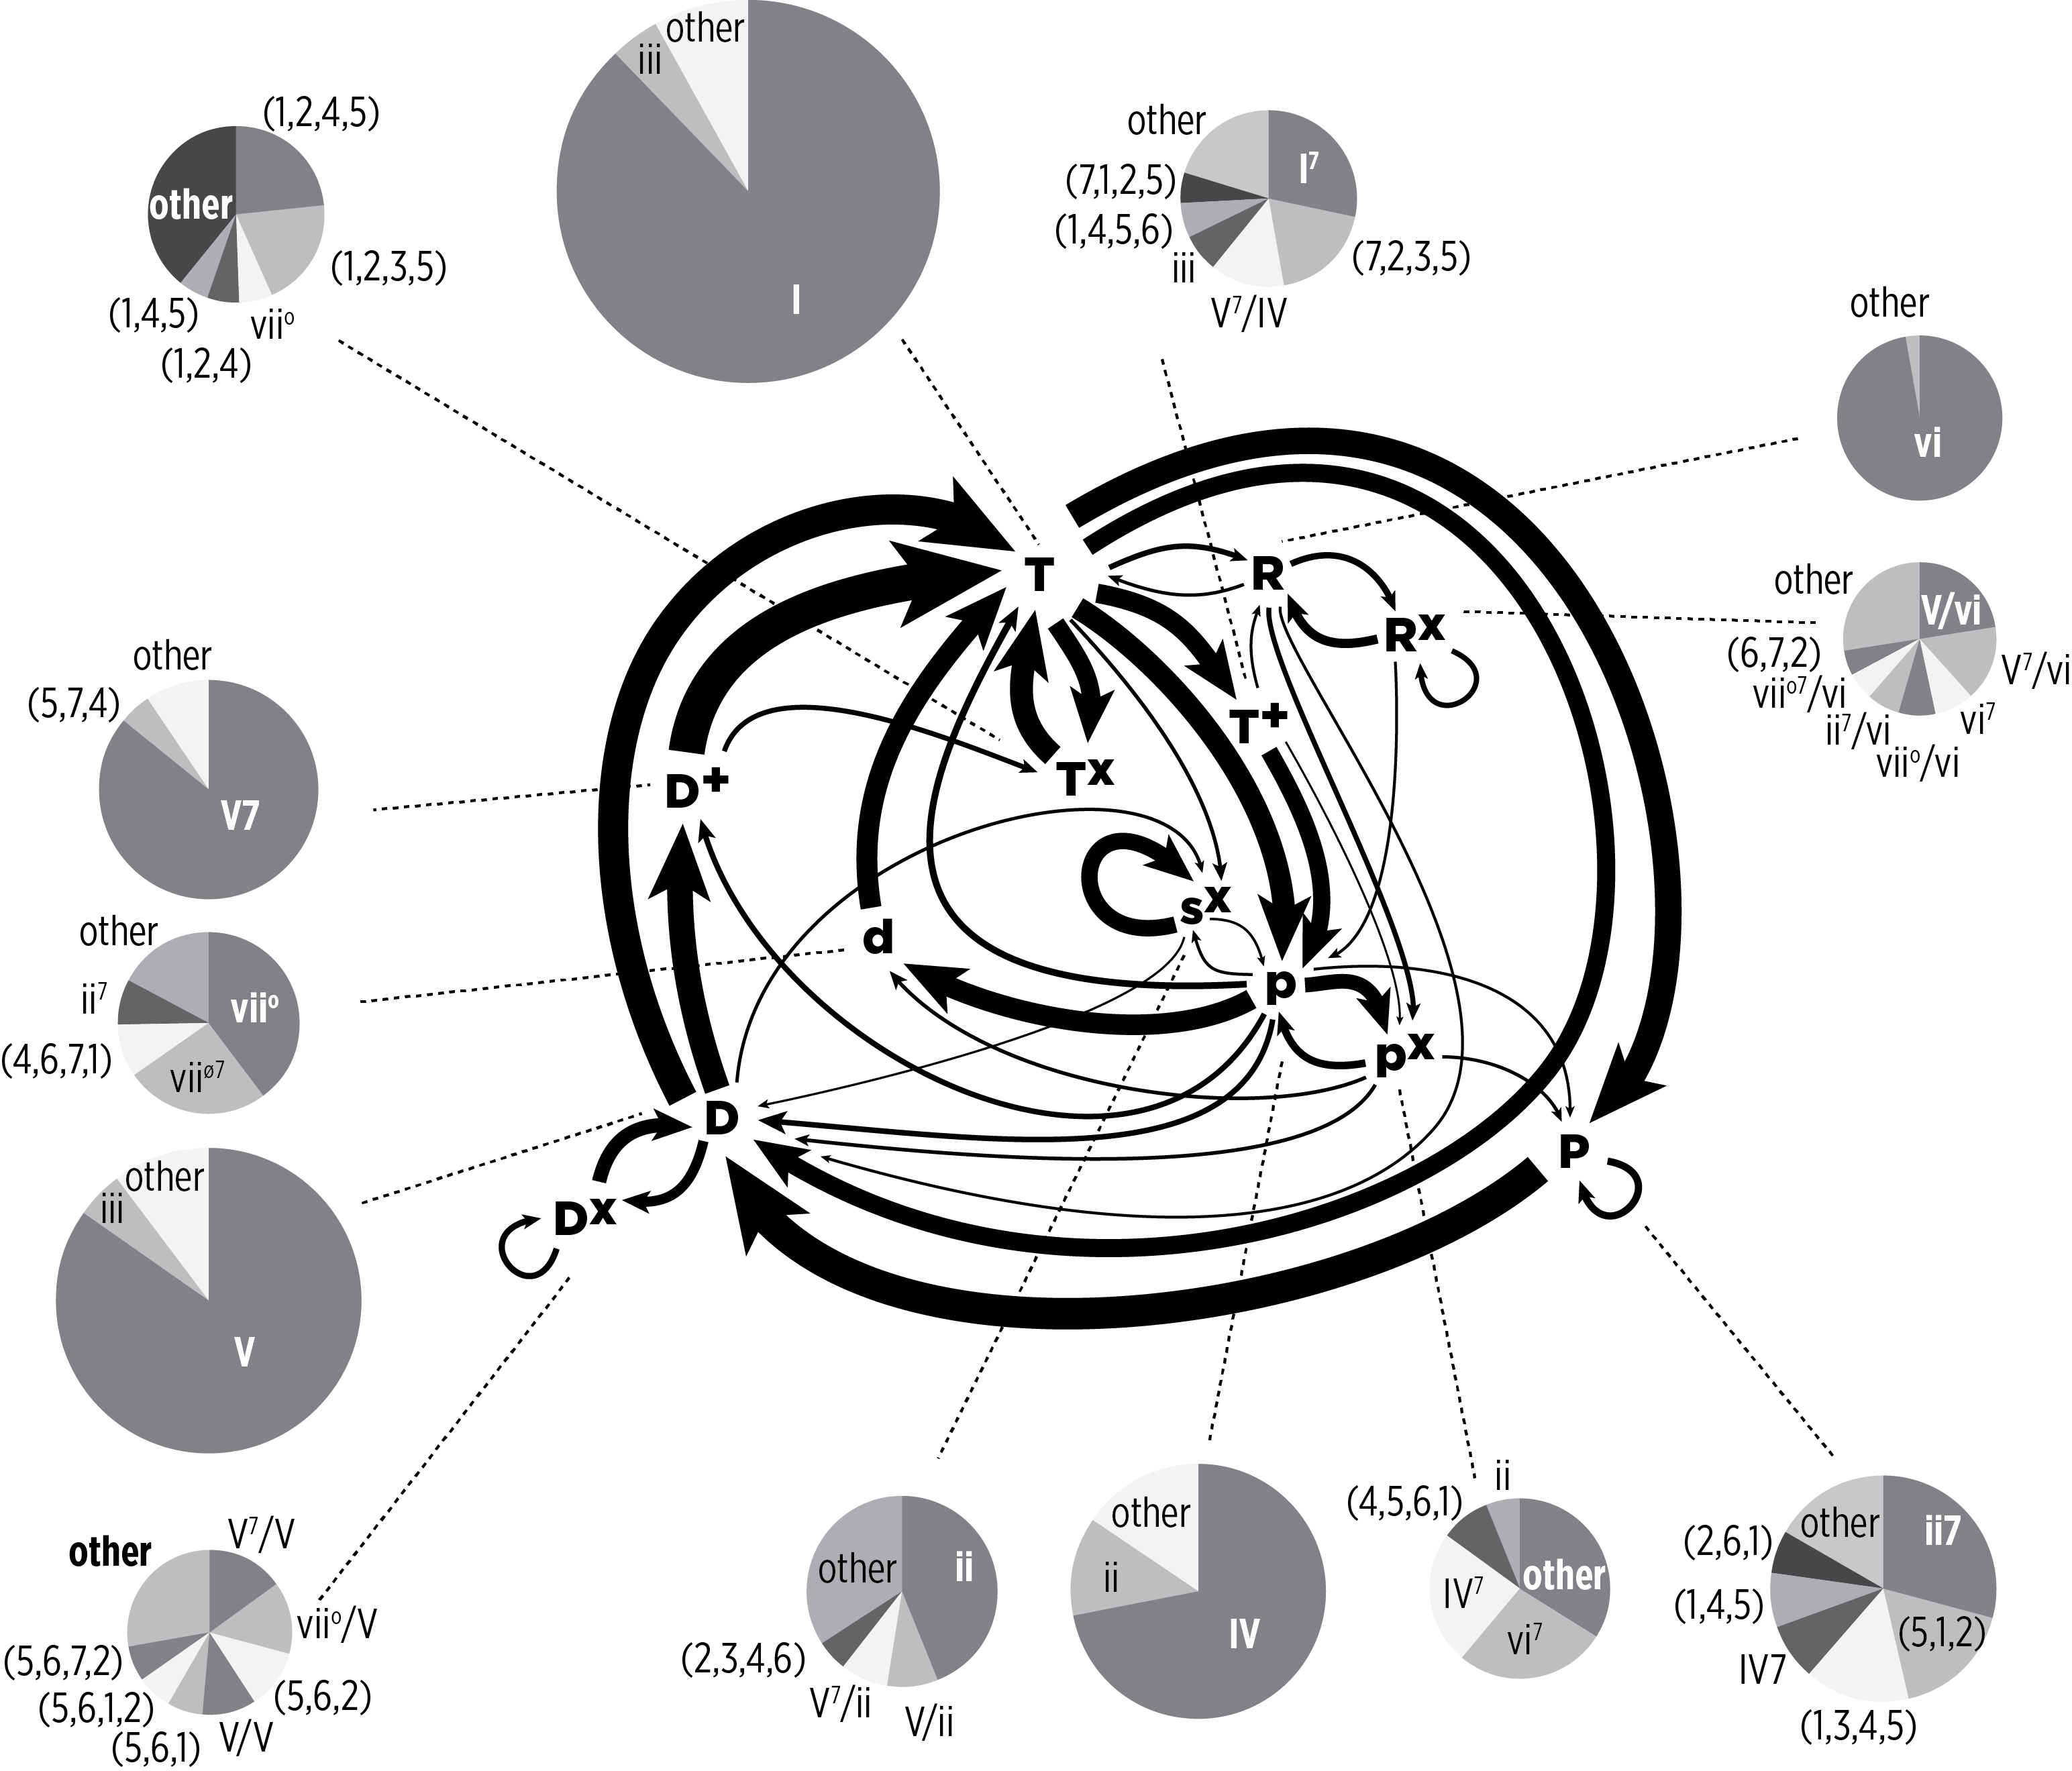
\includegraphics[width=5.5in]{WhiteQuinn_NewPersimmon.png}
	\caption{An empirically-derived ``persimmon" model of functional progression in the Bach chorales, taken from \cite{wq2017}.  Dotted lines indicate chord membership within functional categories.  Solid arrows indicate category-level progressions, whether function-preserving (self-progressions) or not (syntactic progressions).  While this diagram encodes progressions on different time scales, neither the progressions nor the functional categories engage with the temporal structure of the data.}
	\label{pers}
\end{figure}

On its most basic level, the ``persimmon" of Figure~\ref{pers} includes a combination of pitch-based chord labels (roman numerals) and functional categories ($T$, $S$, $D$, $P$, and $R$) linked by a variety of arrows.  For each functional category, the dotted lines on the figure provide a mapping indicating the kinds of chords likely to appear as members of the category.  Between categories themselves, solid arrows indicate common functional progressions.  Some progressions are from one syntactic function to another -- say, $T \rightarrow P$ or $P \rightarrow D$ -- while others indicate ``self-progressions" like $T \rightarrow T^x \rightarrow T$.  Each arrow thus corresponds to a chord transition, an immediately-adjacent bigram, and the actual pitch content of such a transition can be drawn from the pie-chart distributions relevant to each category.

Figure~\ref{iiprog} shows something similar to the solid, functional progression arrows on the persimmon, though it replaces the bigram orientation with a more explicit engagement with time.  While Figure~\ref{pers} indicates that $ii^7$ as predominant (P) frequently progresses to $V$ as dominant (D), Figure~\ref{iiprog} indicates temporal limits to such a claim; at very short and very long time scales, the $ii$ chords captured by Figure~\ref{iiprog} hardly progress to $V$ in any significant way, and it is only in a certain temporal regime that the $ii \rightarrow V$ syntactic progression claim seems to live.

This chapter provides a case study exposing the machinery behind and implications of Figure~\ref{iiprog} and its ability to describe multiple \emph{temporal progression regimes} within a single statistical framework.  Examples of short-timespan self-progressions (like the blue $ii$ curve) and moderate-timespan syntactic progressions (like the gray $V$ curve) motivate the automated extraction of chords to which $ii$ tends to ``progress" at different time scales.  Principal component analysis (PCA), a frequent tool in computational time series analysis, will aid in reducing the temporal complexity of the many possible chords succeeding $ii$ at many possible scales.  A consideration of the most common ways $ii$ chords progress in time will suggest the possibility of ``bootstrapping" our types of progression, unearthing different temporal progression regimes without analytical inputs and directly from the statistical properties of YJaMP's solo piano performances.\footnote{The use of ``bootstrap" here draws on a long computational tradition of responding to a clear problem: if programmatic algorithms generate or load outputs from a series of inputs, how can a system receive the initial impetus to get off the ground?  (For early use of the term in this manner, see \cite{buchholz1953}).  The software term ``booting" seems to draw on the computational prehistory of pulling oneself up by one's ``bootstraps.")  I hand-supply plausible chord categories here, but I intend this as an initial approximation to be modified subsequently by machine learning methods.}  The case study here serves to anchor chord progressions in a temporal framework amenable to computation, and its methods apply to any scale-degree set in the corpus.  As Chapter 4 will indicate, the resulting temporal representation both captures nuanced progression behavior for individual chords and permits the construction of syntactic categories via elementary machine learning.  In the Kockelmanian terms of Chapter 2, the algorithms of this chapter turn scale-degree set signed indices into interpretants well-suited to the algorithmic agents of Chapter 4.

\section{Chords and Time}
%Chord ``behavior" different on different time scales
%Smallest: static, mostly self-transitions, lends itself to phonetic models
%Small: local behavior, mostly voice-leading neighbors
%Middle: ``Syntactic" models apply, here; suppressions (V-IV) and correlations (V-I)
%Large: predictive power recedes to background statistics (X-...-I)

Temporality and probability lie at the heart of Figure~\ref{iiprog}'s presentation of harmonic progressions.  These two concepts are concretized by the introduction of particular harmonic objects.  In the previous section, the term ``chord category" (applied to $ii$, $V$, and $I$) reflects an artificial (but rather conventional) definition of $ii$ as a category which includes the locally-transposed scale-degree sets $[2,5,9]$, $[0,2,5,9]$, and $[0,2,5]$.\footnote{In conventional scale degree terms, these chords are $(\hat{2},\hat{4},\hat{6})$, $(\hat{1},\hat{2},\hat{4}, \hat{6})$, and $(\hat{1},\hat{2},\hat{4})$.  For further details on the production of YJaMP scale-degree sets, see Chapter 2.}  As seen in Chapter 2, these scale degree sets represent the three most common instantiations of western-classical $ii$ chords produced via algorithmic parsing of the YJaMP corpus.  Along similar lines, the $V$ and $I$ categories indicated on Figure~\ref{iiprog} contain ($[2,7,11]$, $[2,5,7,11]$, $[5,7,11]$) and ($[0,4,7]$, $[0,3,7]$, $[0,4,11]$, $[0,3,10]$, $[0,4,7,11]$, $[0,3,7,10]$), respectively.  Machine learning methods will replace these chord category assumptions in Chapter 4, but they appear here as the simplest way to connect functional category concepts from traditional harmony to computational time series analytical methods.

The horizontal axis of Figure~\ref{iiprog} represents time in milliseconds.  Strictly speaking, the plotted probabilities do not provide continuous data; instead, each 50-millisecond time window has been ``binned," where its contents are assumed to be simultaneous enough to warrant consideration as a potential chord in the way outlined at the end of Chapter 2.  The left hand side of the figure, where $t=0$, is the time at which a $ii$ chord appears; $t=500$ is 500ms later (one half second), and $t=5000$ is 5 seconds after the initial $ii$ chord.  Each point on a plotted curve indicates how much more or less likely the curve's chord is to be found $t$ milliseconds after a $ii$ chord than it is to be found in the corpus in general.  A Python algorithm finds every instance of a $ii$ chord in the YJaMP performances and tracks the time delay with which each chord appears in the subsequent 5 seconds.  A kind of composite statistical template results: given $ii$ as an ``origin chord," the algorithm returns a probability distribution for each subsequent 50ms window in which it accounts for every ``destination chord" found that long after a $ii$ chord.  These probability distributions consist of coded versions of claims like ``$t$ milliseconds after a $ii$ chord, chord $x$ appears $y$ orders of magnitude more often than it does in the corpus generally."  

This claim does not reference the absolute probability of appearance for the ``destination" chord $x$ directly, since such a statistic would not make plain the predictive or syntactic importance of $ii$ itself.  A chord highly probable (in absolute terms) at some time $t$ might reflect a high background \emph{unigram} probability independent of the nearby presence of $ii$.\footnote{For further details on the quasi-Zipfian unigram distribution of the YJaMP corpus, see Chapter 2.}  Figure~\ref{iiprog} normalizes these distributions, however, plotting the difference between two logarithmic probabilities on the vertical axis:
\begin{equation}
P(x,t) = \log_{10} \big( p(x\mid ii,t) \big) - \log_{10} \big( p(x) \big)
\end{equation}
Here, $P(x,t)$ is the relative log probability of chord $x$ at time $t$ plotted on the vertical axis of Figure~\ref{iiprog}, while $p(x)$ and $p(x\mid ii,t)$ are the probabilities of $x$ in the corpus at large and given the previous occurrence of $ii$ $t$ milliseconds previously, respectively.  Subtracting these logarithmic probabilities performs a normalization similar to dividing the (non-log) probability-given-$ii$ by the probability-in-general.  The result of the logarithmic normalization is that the positive vertical axis values of Figure~\ref{iiprog} indicate probabilities higher than the background unigram distribution, while negative axis values indicate that the given chord occurs less frequently at a given delay $t$ after $ii$ than it does in the corpus in general -- that the chord is suppressed by $ii$.  Each increase of one unit on the vertical axis corresponds to a particular chord occurring 10 times more probably at a given time $t$ than its unigram probability.

%talk about using these curves as templates for isolating types of progression behavior into different temporal regimes.
If the curves of Figure~\ref{iiprog} show the relative probabilities of three destination chords, they stand as a way of quantifying the effect of the origin chord ($ii$) on the presence of subsequent -- and not necessarily adjacent -- $ii$, $V$, and $I$ chords.  The appearance of $ii$ has one particular kind of effect at short distances: it makes other $ii$ chords much more probable.  But how many chords does $ii$ impact in a similar way, and how many kinds of effect does $ii$ have?

\begin{figure}
	\centering
	\caption{An excerpt of the temporal probability distributions for common chords following $ii$ (unigram-relative log probabilities versus time).  Traditional harmonic theory assumes the ability to reduce this complex temporal data to time-independent category transition rules.}
	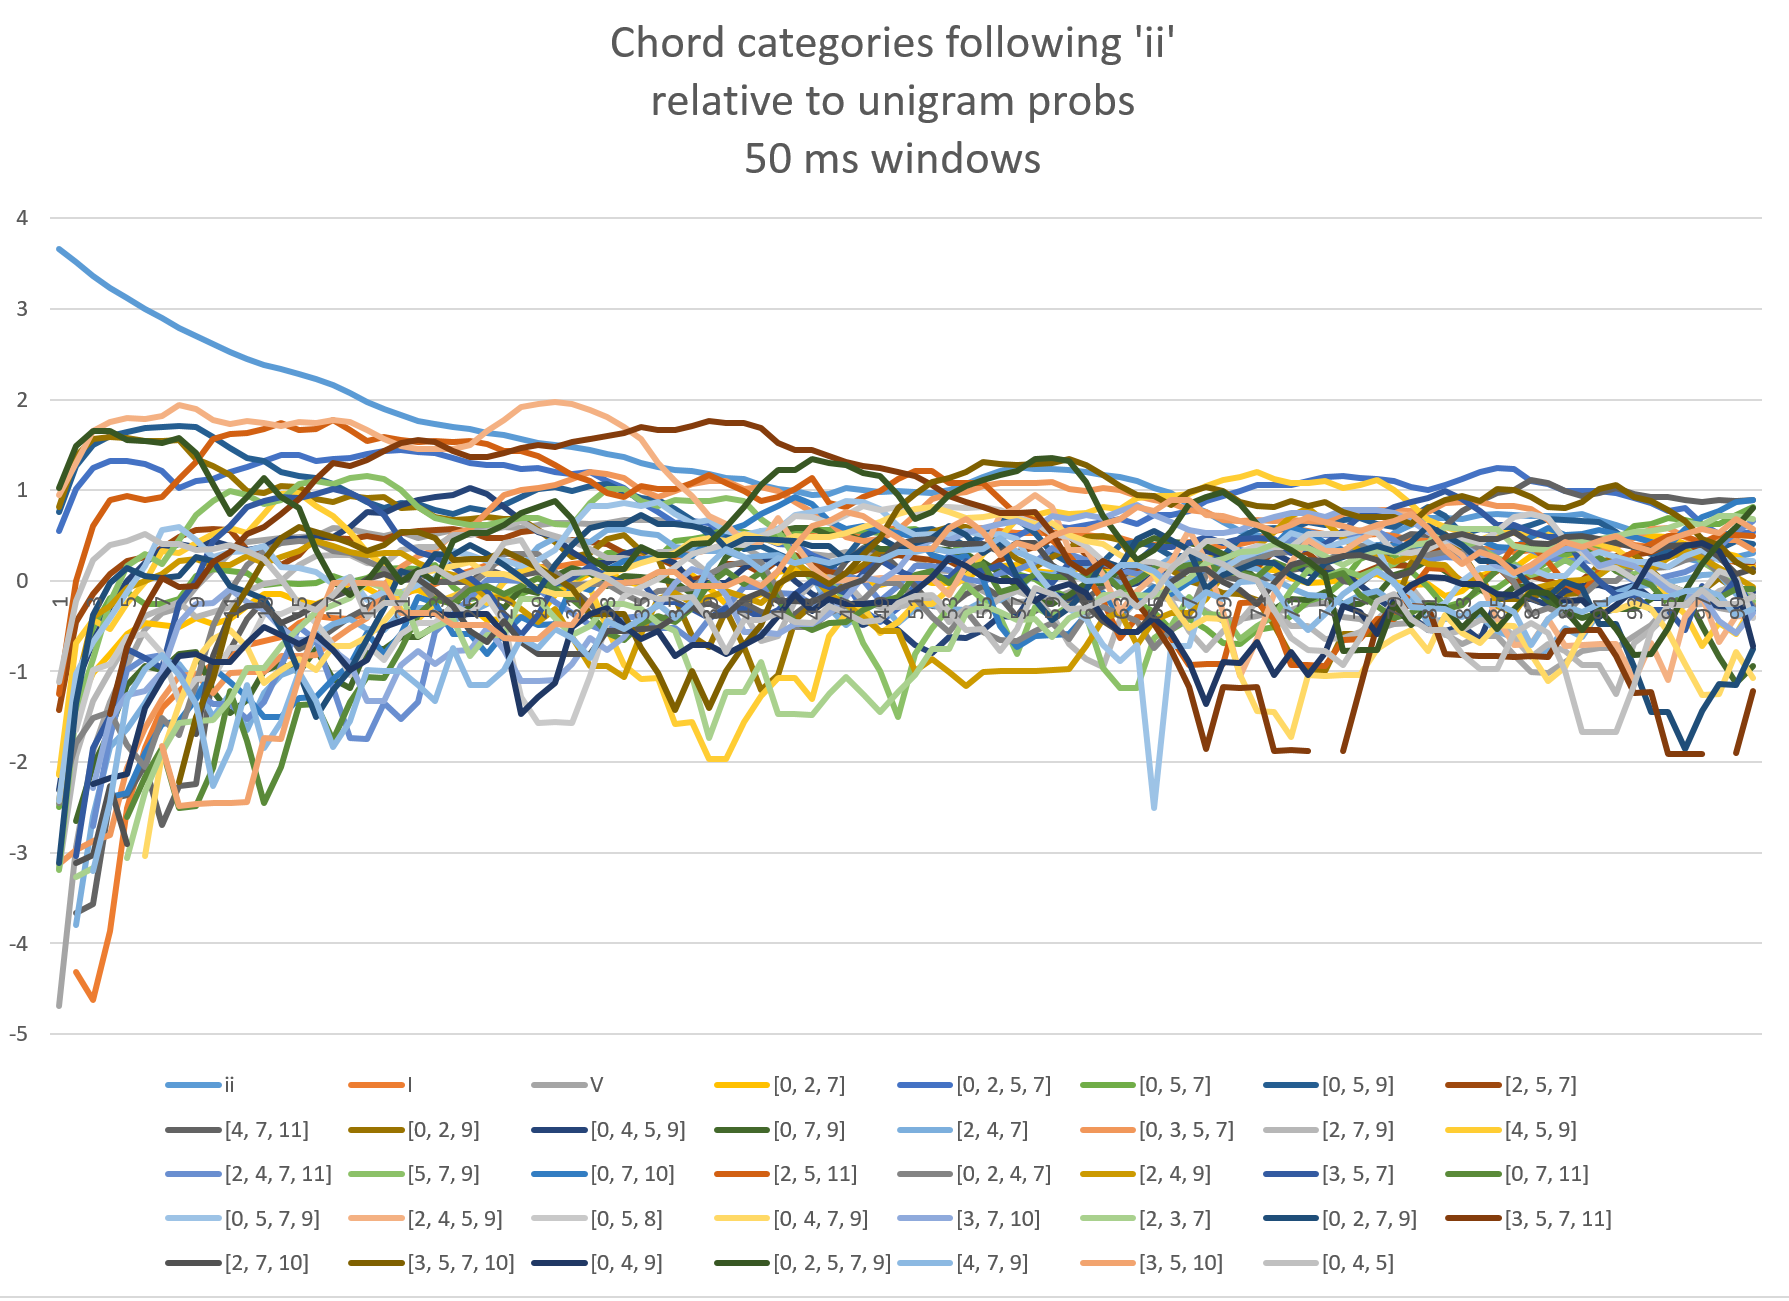
\includegraphics[width=6in]{ii_messy.png}
	\label{ii_messy}
\end{figure}

Figure~\ref{ii_messy} presents a small fraction of the destination chord probability distributions for chords following $ii$.  For many high-probability origin chord types in the corpus (like $ii$), tokens corresponding to more than 1000 distinct destination chord types appear within the 5 seconds following all of the origin chord's tokens across the corpus.  Sorting through these distributions by hand is not feasible, and many of the destination chords are low-probability objects in the first place; there is no guarantee that random fluctuations in the appearance of rare chords will tell us anything about $ii$'s syntactic properties.

But to find other chords strongly impacted by $ii$ in ways similar to the behavior displayed in Figure~\ref{iiprog}, it suffices to compare the large number of destination chord probability distributions to the (blue, gray, and red) templates provided by $ii$, $V$, and $I$.  Curves which lie close to the $V$ curve correspond to chords with temporal behavior similar to $V$ in the context of $ii$.  This sounds tautological, but an important distinction is at play: a chord with a temporal probability distribution similar to that of $V$ on Figure~\ref{iiprog} may have absolutely no discernible pitch relation to $V$ as a scale-degree set.  ``$V$-like" chords, distributionally speaking, need only \emph{act like} $V$, statistically, in the temporal context of $ii$.  In other words, an algorithmic agent calculating which destination chord probability distributions from Figure~\ref{ii_messy} lie closest to those shown in Figure~\ref{iiprog} picks out chords which display temporal behavior similar to self-progressions ($ii \rightarrow ii$), syntactic progressions $(ii \rightarrow V$), and key-appropriate non-syntactic progressions ($ii \rightarrow I$).  This readily automatable process can assemble chord progression categories on more than one time scale -- and it can be performed for any origin chord.

\section{Phonetic scale}
On the shortest of musical time scales, the $ii$ chord tends to predict itself quite strongly, and it does so with diminishing strength as time passes.  To find what other chords behave this way after the appearance of $ii$, a few lines of code iterate across all of the observed destination chord distributions.  For each destination chord $d$, the code sees an $n$-dimensional probability vector, where $n$ can range up to the value of $t/50$ corresponding to the maximum windowed time delay for which statistics are kept.  It compares this vector to the $n$-dimensional ``self-progression" prototype (the $ii \rightarrow ii$ distribution) element-wise, subtracting the log probability of the current destination chord ($p_d$) from the log probability of the $ii$ chord ($p_{ii}$) at each time window.  Summing the absolute value of all of these deviations gives a simple metric for how dissimilar the destination chord is from $ii$:
\begin{eqnarray}
p_{ii} &=& (x_1, x_2, ... ,  x_n) \nonumber \\
p_{d} &=& (y_1, y_2, ..., y_n) \nonumber \\
D_{(ii,d)} &=& \sum_{i=1}^{n} \lvert y_i - x_i \rvert
\end{eqnarray}
That is, the code subtracts the probability of the origin chord $ii$ in window 1 (0-50ms) from the probability of the destination chord $d$ in window 1, takes the absolute value of the difference, and combines the resulting distances over $n$ consecutive time windows.  Setting $n$ is a matter of taste; I have chosen here to compare curves out to where the behavior of the prototype begins to level off.\footnote{As I will discuss below, PCA serves to diminish the importance of any particular choice of $n$, though it is important to track temporal statistics far enough to capture syntactic behavior.}  Minimizing the dissimilarity $D_{ii,d}$ given by Equation (3.1) provides a list of the destination chords which best fit the short-term behavior of $ii$.  A plot of the 5 best destination chords of this type is given in Figure~\ref{ii_phonetic}.

\begin{figure}
	\centering
	\caption{The 5 destination chords for $ii$ progressions with temporal probability distributions most similar to that of $ii \rightarrow ii$ (unigram-relative log probabilities versus time).}
	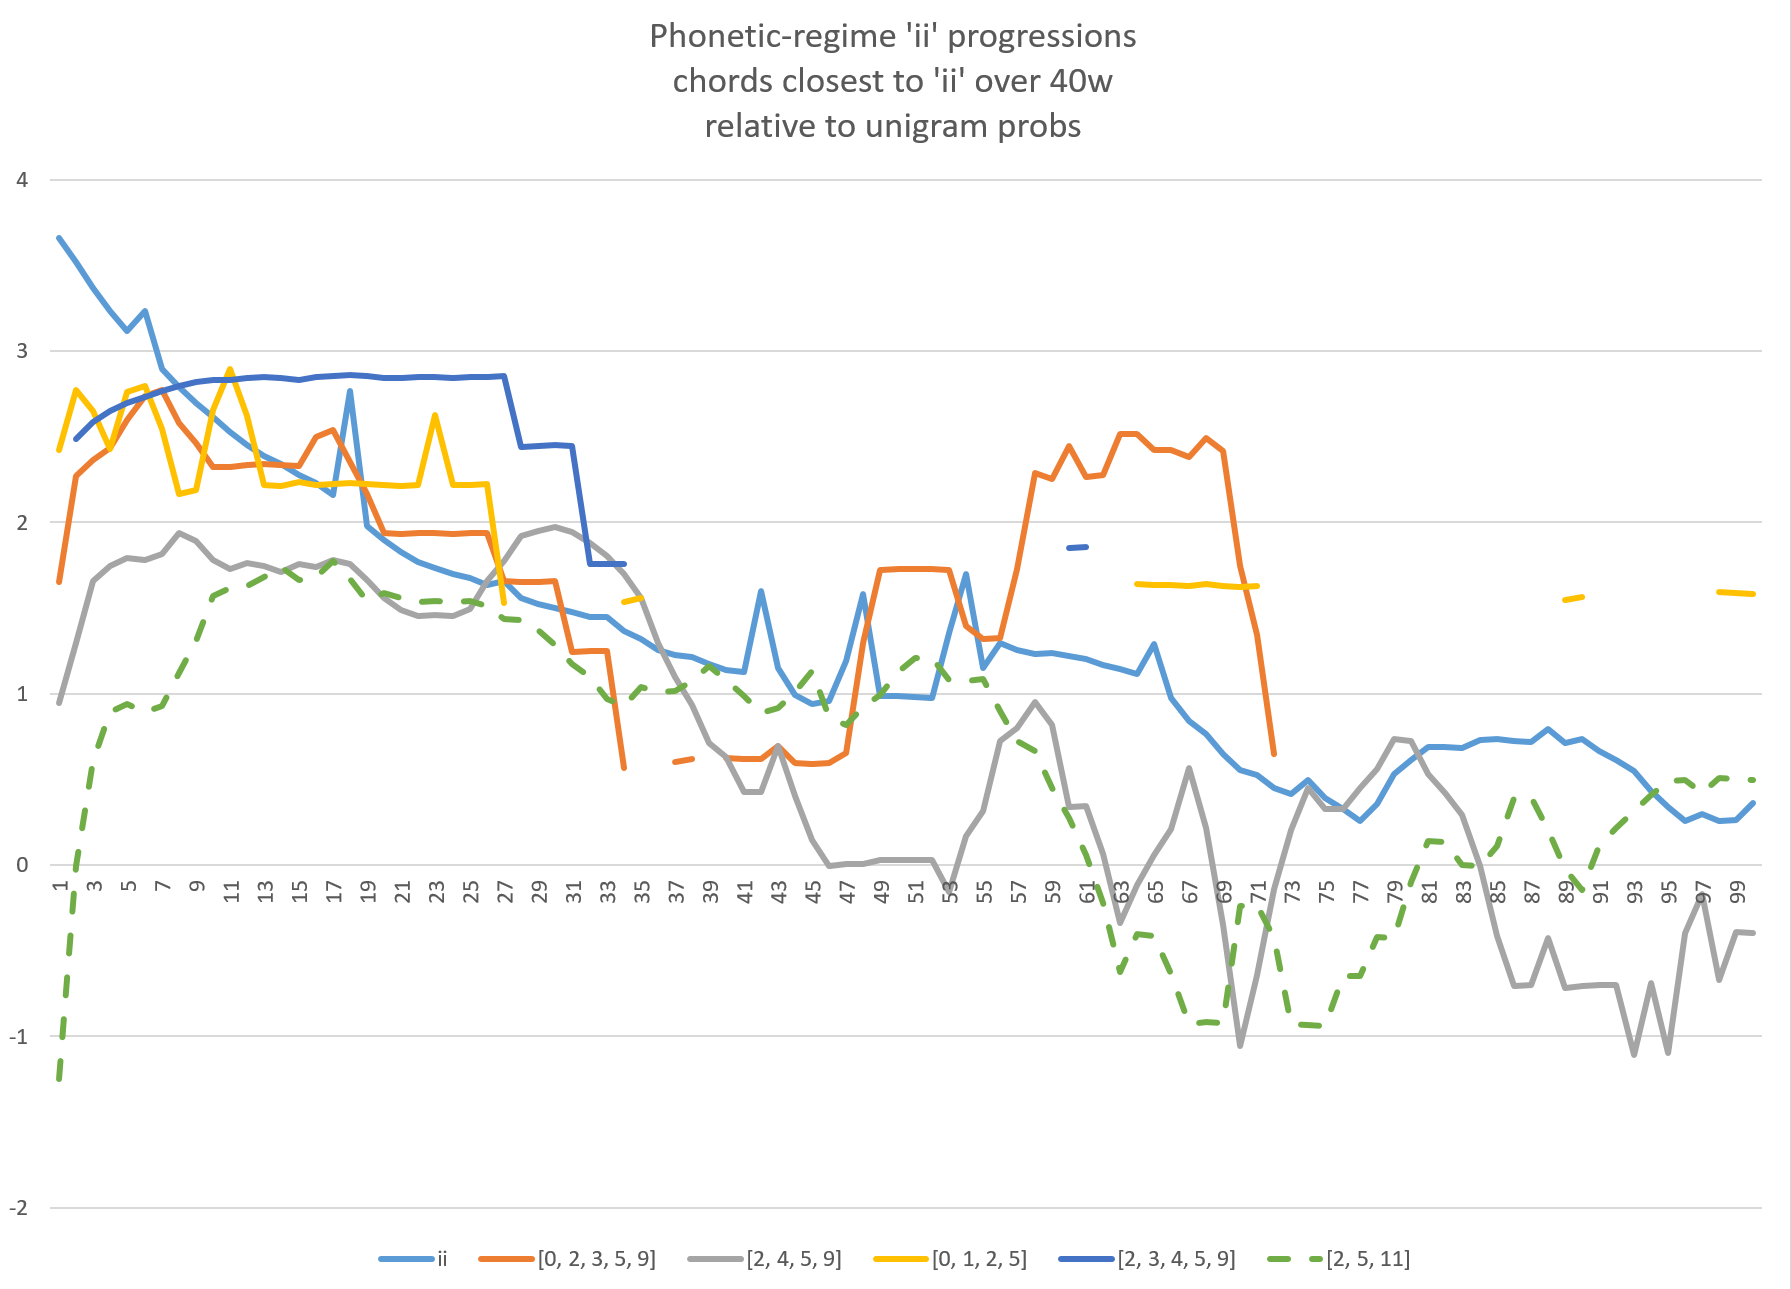
\includegraphics[width=6in]{ii_phonetic.png}
	\label{ii_phonetic}
\end{figure}

The results are striking in their predictability.  While pitch class/scale degree content played no role in the selection of self-progression destinations for $ii$, most of the destination chords with behavior most similar to $ii$ consist of some form of $ii$ chord with one or more added tones. $[0,2,3,5,9]$ and $[2,4,5,9]$ likely draw scale tones from their minor and major tonics, respectively, while $[0,1,2,5]$ and $[2,3,4,5,9]$ appear to arise from some local melodic motion.  In general, the list of self-progression partners for $ii$ suggests two rough categories of behavior:
\begin{enumerate}
	\item The destination chord may be related to the origin $ii$ chord by harmonic or quality completion.  Example: $[0,2,5] \rightarrow [0,2,5,9]$.
	\item The destination chord may be related to the origin $ii$ chord by the introduction of melodic notes. Example: $[0,2,5,9] \rightarrow [0,2,3,5,9]$.
\end{enumerate}
The two types of behavior can be combined, and there are also conditions where a self-progression may ambiguously result from either (i.e., $[2,5,9] \rightarrow [0,2,5,9]$).  In traditional music theory parlance, identifying chord ``progressions" in this context provides an alternate grounding for voice-leading or prolongational reduction rules.

In general, few of the progressions at this time scale consist of transitions which an analyst would deem sufficient to indicate a change of ``chord" or ``function."  Moreover, several self-progressions consecutively might be necessary to fill out all the pitches implied by an analyst's roman numeral.  As a result, I refer to this temporal progression time scale as the \emph{phonetic regime}, by way of analogy to linguistics.  In the way that multiple phonemes might make up a word, multiple self-progressions in this regime might make up a functional chord, and the particular ways in which phonetic regime chords are connected to one another rely on particular choices of voicing and melodic context in much the same way that the surface-level phonetic traces of linguistic syntax depend on the particulars of word order and nearby syntactic partners.  If harmonic syntax is to include primarily progressions from one function to another, then the phonetic regime provides a clean and empirically-grounded sense of the morphological transformations necessitated by concatenating syntactic partners. 

So far, I have avoided mentioning the fifth most $ii$-like member of the phonetic progression regime, shown in Figure~\ref{ii_phonetic}: $[2,5,11]$.  This chord, usually labeled $vii^{\circ}$, is not typically said to have the same function as $ii$.  Its presence on the plot might imply two things: that $[2,5,11]$ may appear as a phonetic neighbor to a more normative $ii$ chord (like $[2,5,9]$), or that destination chord curves this far below the self-progression $ii \rightarrow ii$ prototype begin to behave more like syntactic progression destinations than phonetic ones.  The $[2,5,11]$ distribution of Figure~\ref{ii_phonetic} falls almost exactly midway between the prototype curves for $ii$ and $V$ on Figure~\ref{iiprog}, and its behavior in different contexts might suggest assigning it a dual status, playing a role in the phonetic and syntactic regimes.  I mean the progression regime assignments to be fuzzy, in that limiting cases may exhibit behavior ill-captured by a single regime.

Chord category formation -- the set of decisions regarding what chords should make up a functional, syntactic category -- involves much more than a quick perusal of Figure~\ref{ii_phonetic}.  Comparing destination chord regimes across many (non-$ii$) origin chords provides a much broader data set well-suited to machine learning techniques, the results of which appear in Chapter 4.  To complete the $ii$ temporal progression case study, I turn here to another important time scale implied by Figure~\ref{iiprog}.

\section{Local syntactic scale}
Finding syntactic progressions amounts to a change in time scale.  The previous section showed that self-progression destination chords could be found by calculating which distributions most closely resembled that of $ii\rightarrow ii$ over short time scales, regardless of pitch content.  The same logic applies to functional syntactic progressions: if $ii\rightarrow V$ is a prototypical syntactic progression, destination chords at the time scale of the ``syntactic regime" should have temporal probability distributions similar to that of $V$ over moderate time scales.  Judging from Figure~\ref{iiprog}, the time scale relevant to that behavior stretches out to about 3 seconds.\footnote{Here, again, I describe the time scale cutoff intuitively, assuming that the initial suppression, sharp increase in probability, and return to unigram probability are all features of syntactic-$V$-ness.  It is unclear, in this description, if the lower-probability fluctuations at the end of the temporal tail bear important information; PCA will treat this problem below.}  Comparing all the destination chord probability distributions to $ii \rightarrow V$ over the time domain $(0,3000ms)$, we can again extract those most similar.  The seven best-fitting curves appear in Figure~\ref{ii_syntactic}.

\begin{figure}
	\caption{The 7 destination chords following $ii$ with syntactic regime probability distributions most closely resembling that of $ii \rightarrow V$.  Chords resembling both $V$ (solid curves) and $IV$ (dotted curves) appear to behave similarly.}
	\label{ii_syntactic}
	\centering
	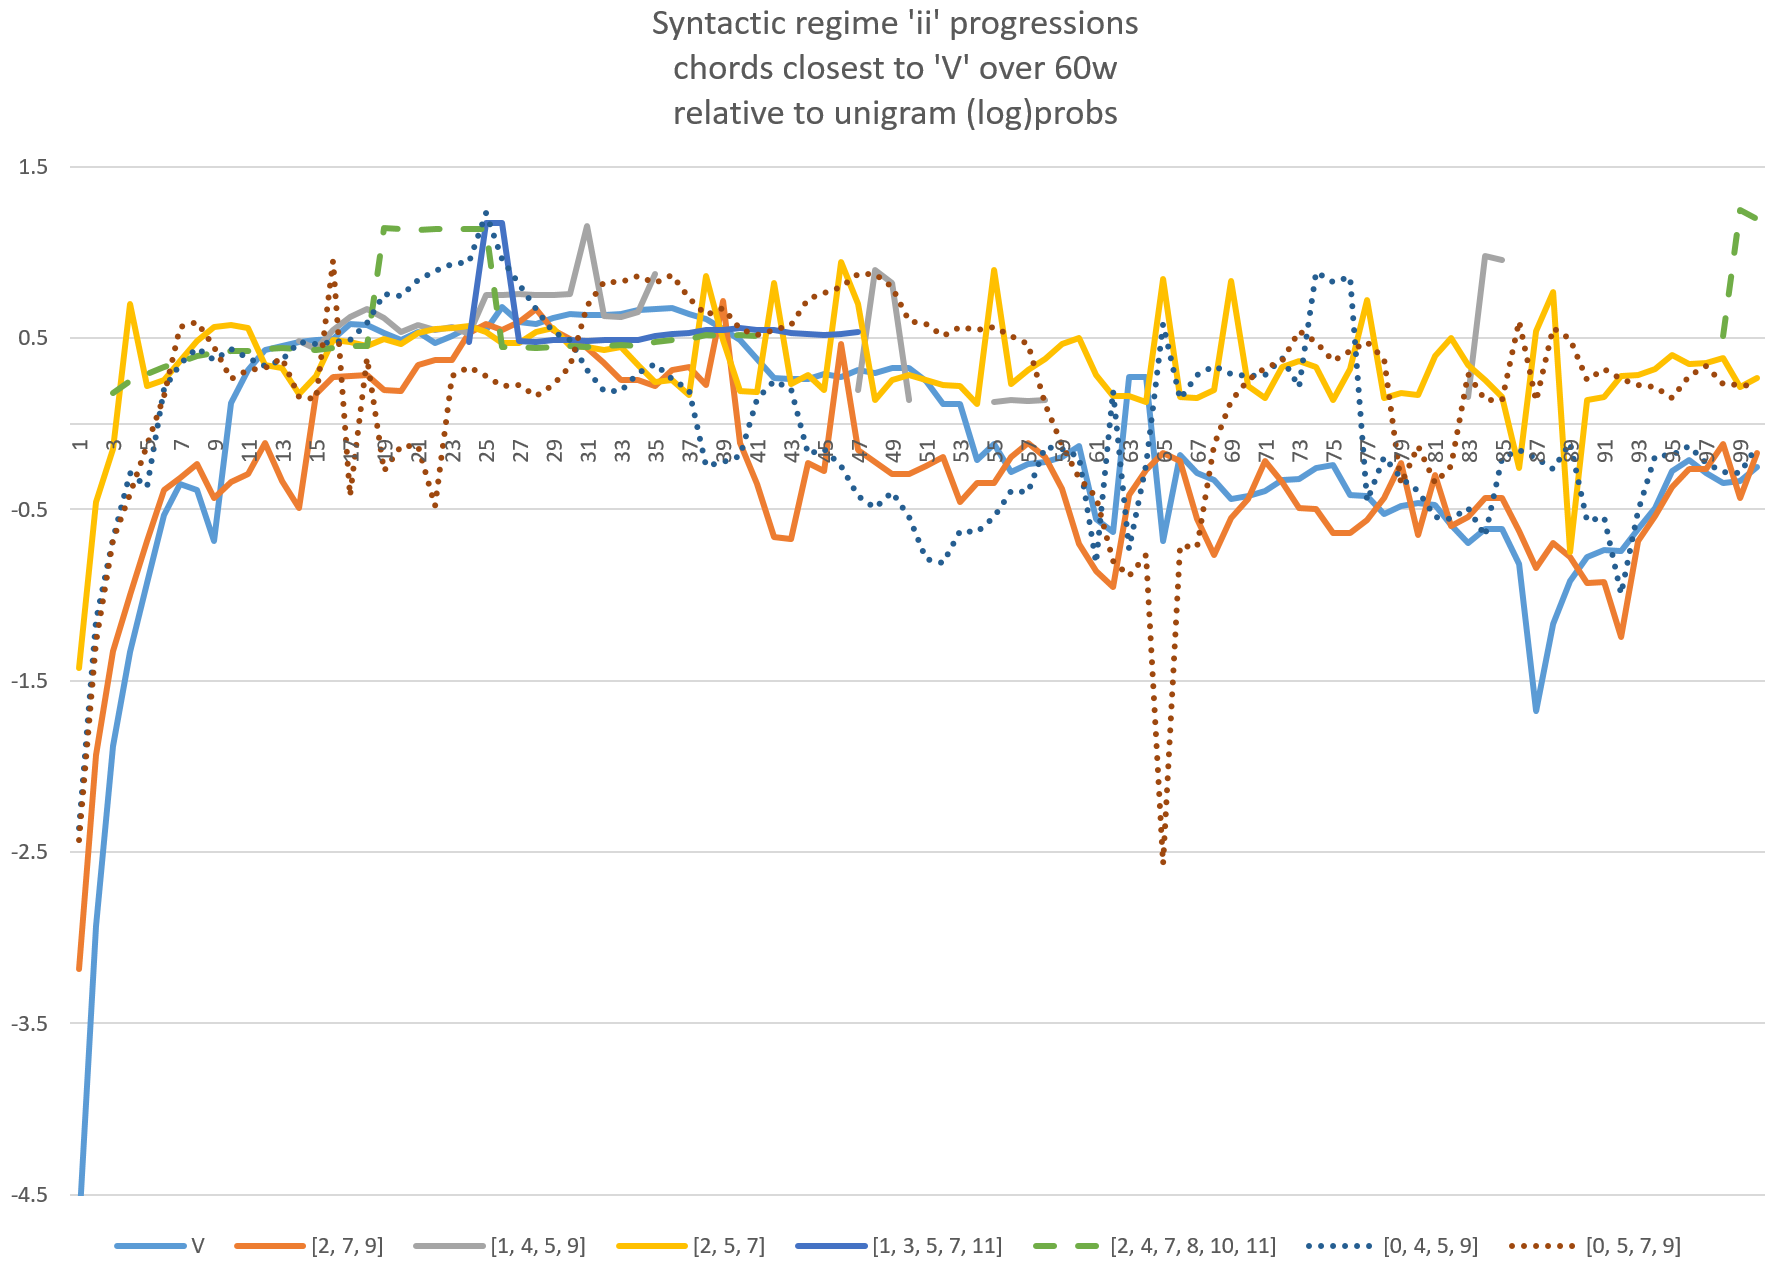
\includegraphics[width=6in]{ii_syntactic.png}
\end{figure}

Many of the destination chords which most closely mimic $V$ in this context are chords we might think of as phonetically-related to $V$ proper (see the solid curves on Figure~\ref{ii_syntactic}).  $[1,3,5,7,11]$ can be parsed as a $V^{\sharp 11 \flat 13}$, and $[2,5,7]$ may function as an incomplete $V^7$.  $[2,7,9]$ might be related to $[2,7,11]$ by melodic step, or it could be a symptom of more complicated behavior in play; $[2,4,7,8,10,11]$ is almost certainly the latter, and I have drawn it with dashes to indicate its ambiguous traditional interpretation.  But the syntactic nature of the $ii \rightarrow V$ curve does more than pick out the phonetic neighbors of $V$.  Since the temporal similarity metric assumes no pitch class or root similarities whatsoever, behavioral similarity also strongly selects another type of chord likely to follow $ii$: $IV$ chords.  Shown in the dotted curves of Figure~\ref{ii_syntactic}, $[0,4,5,9]$ and $[0,5,7,9]$ are both likely to follow $ii$ in a way similar to $V$ -- both types of chord would be deemed syntactic if found a moderate time after $ii$.

In this way, syntactic regime progression data partly reproduces and partly cuts across traditional functional harmony expectations.  Crucially, not all chords which behave like $V$ after $ii$ will \emph{always} behave like $V$; in other origin chord contexts, their behavior might be highly differentiated.  Each possible origin chord provides a distinct set of phonetic and syntactic data which might be used for functional categorization.  The $ii$ syntactic data here indicates a category of ``chords which follow $ii$ at moderate delays," of which both $IV$ and $V$ are members, but other syntactic data might distinguish the two.  In the context of $V$ origin chords, for example, the two fall into generally distinct regimes.  As Figure~\ref{V_phonetic} indicates, $V \rightarrow V$ is a phonetic-type progression, and in this regime, no chords resembling $IV$ are probable.

\begin{figure}[h]
	\caption{Phonetic regime self-progression destination chords following the appearance of $V$.  The pitch structure of these chords resembles that of $V^{(7)}$, but they appear here exclusively because their temporal statistics are most similar to those of $V \rightarrow V$ progressions.}
	\label{V_phonetic}
	\centering
	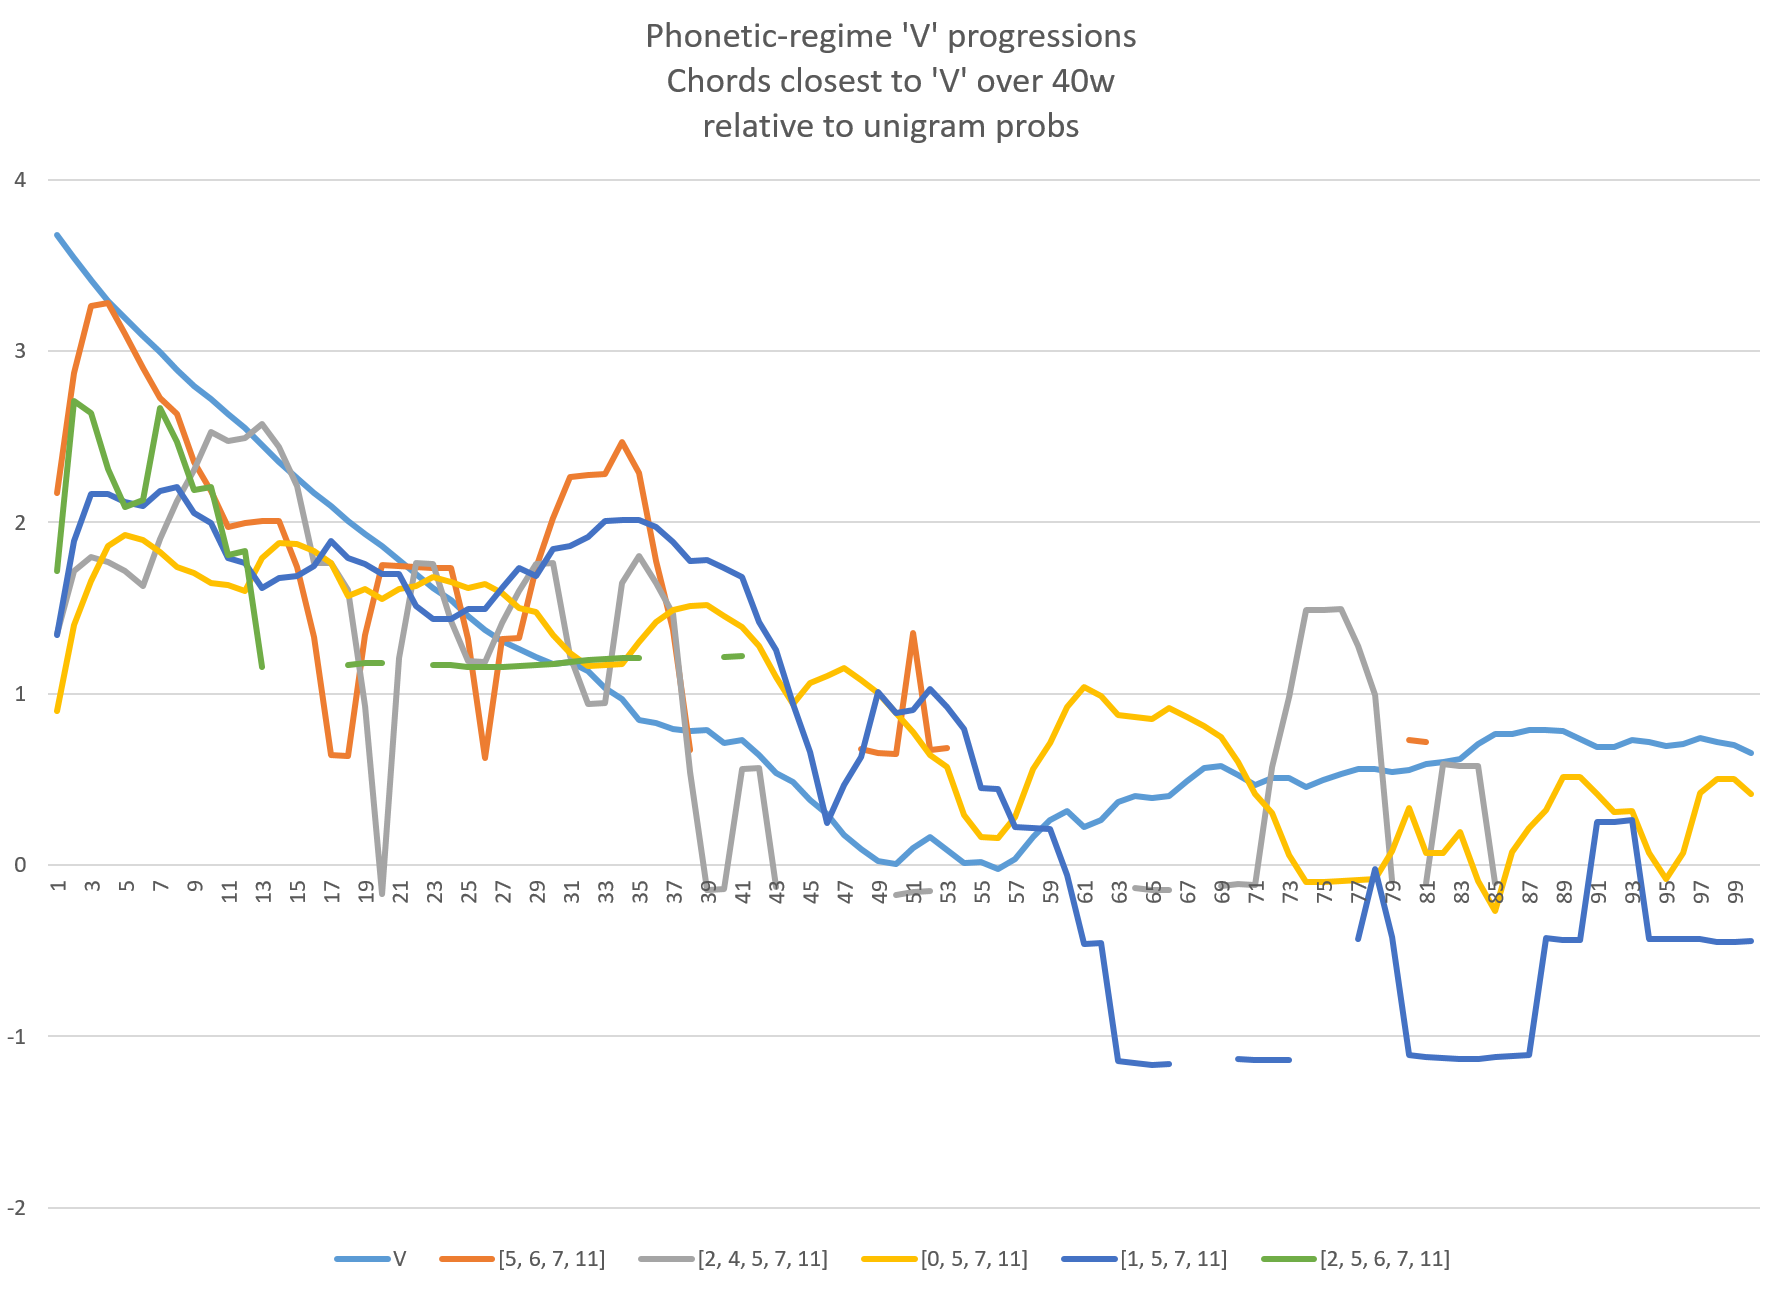
\includegraphics[width=6in]{V_phonetic.png}
\end{figure}

Syntactic regime progressions resembling $V \rightarrow I$, on the other hand, do include chords resembling $IV$, as shown in Figure~\ref{V_syntactic}.  Here, chords with temporal statistics similar to $V \rightarrow I$ cut across traditional functions and roots.  The dotted curve, $V \rightarrow [0,5,7,9]$, resembles blues progression-type motion to a $IV$ chord with an added \nth{2} or \nth{9}.  The solid curves depict ``tonic" type chords $[0,4,7,9]$ and $[0,2,3,7]$.  A human analyst might interpret the former as $I^6$ or $vi^7$, depending on its voicing, while the latter resembles a $i$ chord with added \nth{2} or \nth{9}.  But these ambiguous roman numeral assignments are unnecessary: algorithmically, these scale-degree sets participate in $V \rightarrow x$ progressions highly similar to $V \rightarrow I$, and the category of such progressions constructed here is not based on any particular chord label or root.  Figure~\ref{V_syntactic} implies other frequent progressions, as well: the red dashed curve depicts $V \rightarrow \flat III^{(M)7}$, a ``Giant Steps"-like major third progression (albeit to a major-seventh chord), while the yellow dashed curve indicates that the minor triad $[2,7,10]$ can follow $V$ in a way similar to the other destination chords plotted here.  This last progression may violate the expectations of a human analyst, indicating a site for more detailed, tune-level analysis to determine what kind of behavior is captured here.

\begin{figure}[h]
	\caption{Syntactic regime destination chords following the appearance of $V$.  Note the comparatively short time delay; $V$ does not have a strong predictive impact on the appearance of $I$ for long.  This is likely due both to the very high unigram probabilities of $I$ and $V$ and to $V$'s role in faster progressions (compared to $ii$).}
	\label{V_syntactic}
	\centering
	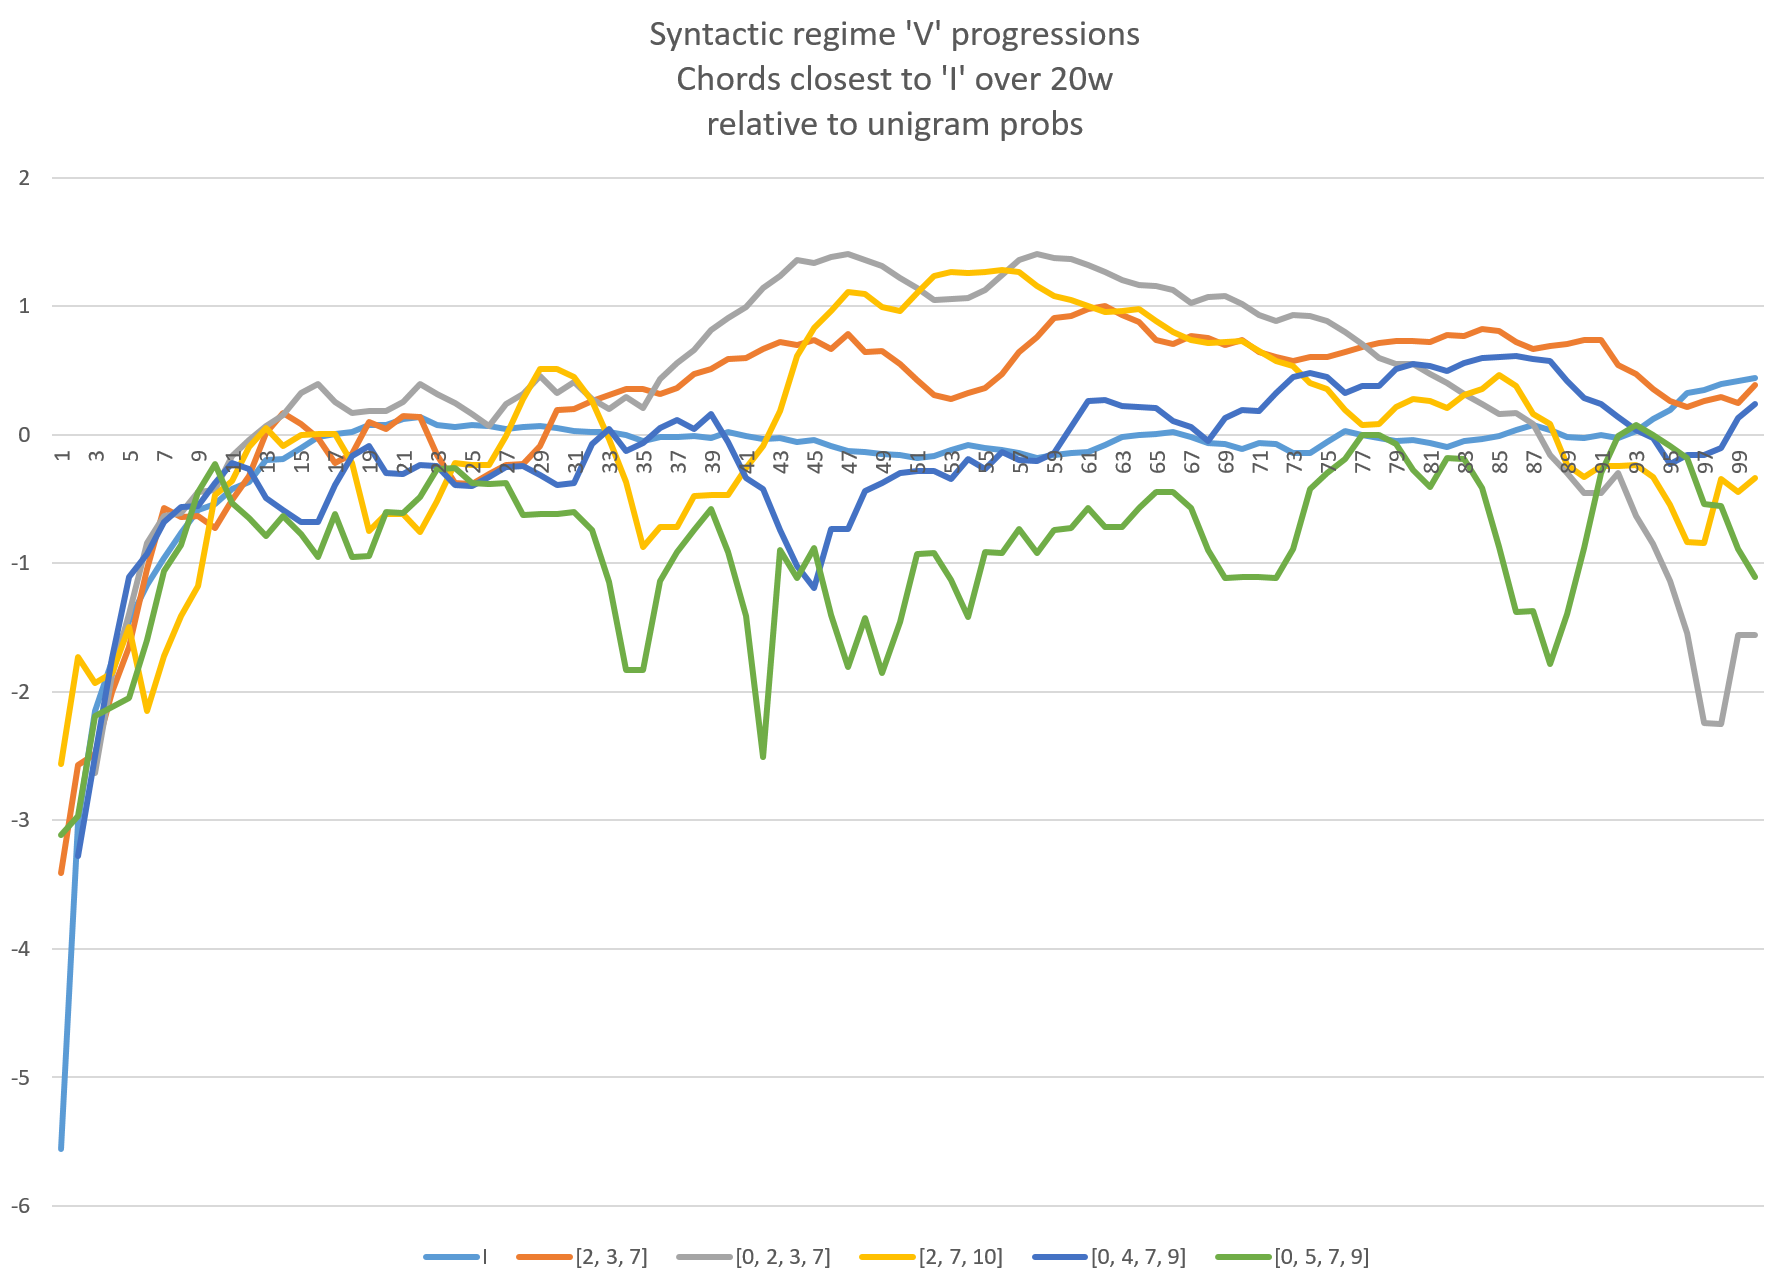
\includegraphics[width=6in]{V_syntactic.png}
\end{figure}

Approaching the phonetic and syntactic regime progressions which resemble prototypical progressions like $ii \rightarrow ii$ or $ii \rightarrow V$ for a variety of origin chords reveals a complex array of progression behaviors both expected and unexpected by a (or this) human analyst.  In these cases, interpreting a syntactic pattern from the temporal correlations between chord states involves communication between algorithmic agents and human agents with different ontological conditions for chords, keys, and progressions.  I will return to this communicative semiotics in Chapters 4 and 5.  But part of the interpretive confusion stemming from the above figures rests on their use of hand-assembled chord categories with labels like $ii,V$ and $I$.

The algorithmic agents tallying temporal statistics and extracting similar probability curves have no particular reason to identify or employ these hand-assembled categories; at the beginning of this chapter, I \emph{posited} them in order to motivate my re-description of traditional harmonic progressions in temporal terms.  But with a sense of how the temporal progression regime behavior of chords might inform syntactic category formation, Chapter 4 will use dimensional reduction and machine learning to construct new chord categories without appeals to roman numerals, root, or pitch similarity.  To enable the algorithmic agents of Chapter 4 to engage with the temporal properties of YJaMP scale degree sets, the remainder of this chapter will generalize the temporal progression regimes of the $ii$ case study above to enable their automated extraction without the necessity of \emph{a priori} intuitive prototypes.

\section{Temporal Progression Regimes}
The selection above of $ii \rightarrow ii$ and $ii \rightarrow V$ as prototypes for categories of temporal progression behavior served an important purpose.  Since probabilistic statistics connect each origin chord to a large number of destination chords, some principled method for selecting destination chords with common behaviors is necessary.  The examples used in this chapter depend on thousands of 100-dimensional vectors, each of which features its own unique shape.  Choosing temporal progression prototypes constituted a selection of shape types.  I assumed that the shapes of the $ii \rightarrow ii$ and $ii \rightarrow V$ chord distributions were common and important ones.  But the YJaMP data can suggest its own collection of shape types.

Principal component analysis (PCA) treats problems of exactly this nature in the world of time-series analysis and machine learning.\footnote{Common in the machine learning literature, PCA dates to \cite{pearson1901}.  Other machine learning techniques accomplish similar ends, and I have no proof that PCA provides optimal results -- but the structure of the time-series analytical problem here, with its presumed near-continuity between adjacent time windows, suggests the appropriateness of the tool.}  Given a data set with a high-dimensional coordinate basis -- like a set of 100-dimensional vectors -- PCA constructs a lower-dimensional coordinate system, projecting elements of the data set onto a much smaller collection of new basis vectors which best account for a maximum amount of the variance in the data.  The formal details are complex, but I offer an intuitive explanation here to connect temporal progression regimes to the PCA results.\footnote{PCA receives formal treatment in textbooks like \cite{jolliffe2002}; see especially its application to time series analysis in Chapter 12, pp.\ 299 ff.  Music theoretical projects employing PCA appear in rhythm and microtiming studies (\cite{repp1992}; \cite{benadon2015}), while the Music Information Retrieval (MIR) community applies it to extracting harmonic information and genre features from complex audio signals (see \cite{huang2014}; \cite{kaneko2010}).  My use here draws on features of both approaches.}

PCA algorithms treat a collection of observations as a sample population.  The individuals in the sample -- all the destination chords for a given origin chord like $ii$, in this case -- vary in their properties, and some are more alike than others.  After the appearance of $ii$, some destination chords will show large spikes in probability in the first few time windows compared to their corpus-wide unigram properties.  Consider how much more likely $[2,4,5,9]$ is to appear within 1.5 seconds after $ii$; Figure~\ref{ii_phonetic} indicates that it appears at this time scale almost 100 times as often as it does in the corpus at large.  But at time delays longer than about 2 seconds, $[2,4,5,9]$ displays much smaller increases in probability over its unigram statistics, crossing back and forth across 0, the value corresponding to no change from the unigram probability.  Since many phonetically-unrelated destination chords show much smaller (or nonexistent) probability spikes at this time scale, the set of all destination chords for $ii$ displays significant \emph{variance} across the first few time windows -- variance typically correlated from time window to time window, since a chord with high probability at 50ms is also likely to have a similarly-high probability at 100ms.

Conversely, at time delays beyond a few seconds, the set of destination chord probability distributions for $ii$ shows comparatively little variance, since the appearance of $ii$ has only a small impact a chord played much later.  This observation reflects the tendency on each of the log-probability plots above for destination chord probability curves to level off near zero over time.  Syntactic-regime destination chords might display yet a third kind of variance, since their probabilities might display large spikes further out in time than phonetic-regime chords and leveling off toward low-variance at later times than syntactically-unrelated chords.  The presence of many destination chords displaying these temporal behaviors will cause the overall set of all destination chords to display different patterns of temporal variance, templates capturing ways of varying in time.  PCA attempts to extract these templates by examining what combinations of time windows tend to vary together the most across the set of destination chords.  PCA ``thus can reveal whether there is more than one shared timing pattern represented in the sample," more than one way of varying over time in the presence of $ii$.\footnote{\cite{repp1992}, p.\ 240.  While Repp describes PCA in the context of expressive timing, his description of ``shared timing patterns" is still apt, here.}

Outside the temporal domain, PCA affords a geometric interpretation.  In the case of the destination chord probability distributions for $ii$, an algorithmic tallier has assigned each observation in the sample 100 coordinates, probability scores in each 50ms time window out to five seconds.  We might, with some imagination, think of each destination chord as a single point in a 100-dimensional space; the full set of $ii$'s destination chords, then, would be a cloud of such points.  Along some coordinate dimensions in that space -- like the coordinates corresponding to long times after the appearance of $ii$ -- the points of the sample cloud will be close together.  Along other dimensions, like the coordinates corresponding to very short times, the points might be quite spread out.  PCA rotates the space in which this cloud lives, identifying the ``principal axes of the ellipsoid that best approximates the cloud of data points... which coincide with the directions of maximum relative variation of the data."\footnote{\cite{benadon2015}, p.\ 25.}

The longest axis of the ellipsoid will be the direction along which the sample displays the greatest variance -- and we could imagine trivial cases where that direction is exactly aligned with one particular coordinate dimension.  If the destination chord probability distributions were identical at all time scales except for the very first time window, the direction of the first coordinate axis would account for \emph{all} of the variance in the data.  PCA could then produce a new set of coordinates which discarded 99 of the axis variables without losing any information about the differences between the distributions.  But for the actual YJaMP progression data, the distributions usually vary over all 100 time scales, many of which are non-trivially correlated.  It might be that chords in the phonetic regime primarily vary over 20 windows, and that the variance in each of those windows is strongly correlated.  If those variances are similar, a PCA algorithm will select as a basis vector -- a direction of the ellipsoid approximating the cloud of points -- some linear combination of the original axes that is maximally aligned with the direction of greatest variance.

After identifying the new axis along which the variance is greatest, the first ``principal component," PCA repeats the process to identify the other highest-variance axes such that the resulting coordinates are still independent and orthogonal.  Each further principal component calculated will capture a smaller share of the overall variance in the population, and an analyst can choose the point of diminishing returns: if 20 coordinates capture 99\% of the variance between 100-dimensional observations (like our destination chord probability distributions), the analyst has little reason to introduce the complexity of an additional 80 coordinates.  This optimized reduction in coordinate complexity is one primary benefit of PCA; the production of template-like principal components is another.

For our case, the principal components can provide automated, data-driven indications as to what different kinds of temporal progression regime there might be, and they present shape types indicative of the types of variance to expect.  Running PCA on the large number of destination chord probability distributions for $ii \rightarrow x$ decomposes the high-dimensional time-based coordinates into a low-dimensional basis of temporal progression regimes.\footnote{Many commercially available standalone software packages offer PCA support.  The implementation I employ in Python comes from the package scikit-learn.  See \cite{scikit-learn}.}  Figure~\ref{ii_pca} plots the first 5 machine-generated principal components for $ii$ chord destinations.

\begin{figure}
	\centering
	\caption{The top 5 principal components calculated from the full set of destination chord temporal probability distributions following $ii$.  The plot is of probability versus time; the legend indicates the components and their variance percentages in descending order.}
	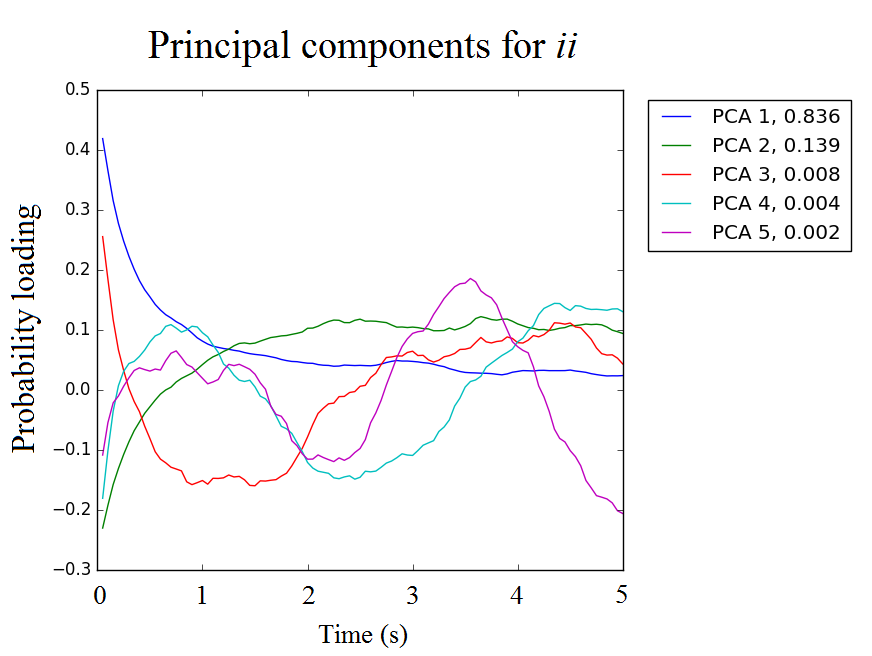
\includegraphics[width=6in]{iipca_ABS_ed.png}
	\label{ii_pca}
\end{figure}

With slight theoretical adjustments, I propose that these distribution shape classes (or, more properly, combinations thereof) can be used in place of the hand-picked $ii$, $V$, and $I$ shape templates employed earlier in the chapter for the assembly of phonetic and syntactic progression regimes.  The first principal component, the blue curve on the figure, accounts for most of the variance in the distributions; large positive and negative scores with respect to this component indicate behavior where the shorter time spans vary much more than the longer ones, which approach their unigram probabilities.  This behavior is comparable to that of the phonetic regime.  Component 2, the green curve, captures chords with large initial variance, but which level off at a non-zero log probability relative to their unigram statistics.  Chords with large positive coordinates along this component are initially suppressed but predicted later, much like non-phonetic chords that do have tonal relevance to phrases in which $ii$ appears (compare this to $ii \rightarrow I$ on Figure~\ref{iiprog}).  Components 3-5 indicate more nuanced variance behavior, though they only account for a very small percentage of the data's variance: as indicated by the legend, the lion's share of information is captured by the first two components.  Component 3, for example, resembles the exact opposite of the $ii \rightarrow V$ syntactic regime prototype.  Multiplying this component by negative one yields a template which starts with phonetic-regime probability suppression, rises to a probability peak between 1 and 2 seconds, and then falls toward the unigram probability. 

To a human analyst, these machine-generated regimes of chord behavior might seem to provide a framework subsuming both ``embellishing" and ``harmonic" progressions -- a general statistical basis for temporal progression behavior.  They rely on no particular knowledge regarding the pitch content of the chords involved, and they suggest a crude binary: that the kinds of chords traditionally reduced away as voice-leading neighbors or functional prolongations might be those which most resemble PCA component 1, while chords identified as part of syntactic progressions might score low along component one and higher along some other appropriately shaped component.

In some cases, this may be true, but it offers no proof or disproof of traditional reduction techniques.  As Chapter 4 will indicate, interpreting these components in isolation requires caution, since destination chords can be described by positive and negative multiples of each component as well as combinations of more than one.  For any given origin chord, the relationship between its principal components and reduction or progression expectations may be less clear than for the $ii$ case study presented here.  With this in mind, the immediate interpretive payoff of the components for a human analyst, though suggestive, is comparatively small.

But I will argue that the algorithmic payoff for a pipeline producing syntactic categories is large: describing an origin chord in terms of the most common ways its destination chords progress in time allows algorithmic agents to use temporal progression statistics as the basis for chord category formation.  Moreover, it does so in a way free of the bigram-like state-to-state transitions assumed in score-based, roman numeral adjacency models of harmonic syntax.  In a sense, time series analytical PCA allows the algorithmic agents to take advantage of much more information than would be encoded in merely adjacent progressions.  Generalizing across temporal regimes widens the scope of harmonic progression inquiry without invoking recursive grammars, Schenkerian prolongations, or pre-determined surface reduction rules.%this is the progressions chapter (based mostly on the ii case study)
\chapter{Clustering, similarity, and learned harmonic categories}
%Intro: claim I'll show how to extract functional syntactic clusters without assuming time scales or pitch relationships
In the last chapter, I illustrated one way to read different types of temporal progression out of statistics for hand-assembled chord categories that I labeled $ii$ or $V$ or $I$.  Given a group of ``origin chords" captured by one of those category labels, I isolated expected ``destination chords" and investigated the differences between their temporal probability distributions.  By the end of the chapter, I was in a position to ask: can we extract this type of information without knowing in advance which origin chords, destination chords, and types of temporal progression are important?  Put in computational terms, can we bootstrap both the chord categories and the temporal progression regimes?

The methods necessary to answer questions of this nature lie at the heart of the project laid out in these pages.  In chapter one, I attempted to show a circularity embedded in analytical-reductive descriptions of musical syntax employed by Lerdahl \& Jackendoff, while chapter two responded to the circularity Robert Gjerdingen identifies in a range of corpus analytical projects.  If harmonic syntax can be extracted from a corpus of performance in a non-circular way, I claim that it should be \emph{learned}, in a computational sense.  This chapter will show what a data-driven, minimally-circular pathway to syntax extraction might look like, while the concluding chapter to follow will question the benefits (and possibility) of syntactic models of a variety of types.

Running PCA on the full temporal probability distribution set for a hand-assembled origin chord category ($ii$, in the preceding chapter's case) implied that the most salient temporal progression regimes can be identified through unsupervised machine learning.  This chapter extends that observation to the formation of origin chord categories, applying similarity measures to a set of origin chord properties with careful choices of metric and basis.  Ultimately, I show that performing flattened agglomerative hierarchical clustering on PCA-reduced temporal probability distributions produces categories of chord similarity which reflect the temporal properties of the data in a robust and sensitive way, reproducing traditional notions of chord similarity and providing a framework for supportable claims of harmonic syntax.  Moreover, supervised classifier models based on the resulting category assignments indicate the potential for exploring and tagging low-probability chords.

\section{Temporal Probability Distributions: From curves to matrices}
%This step isn't formally necessary(?), but it'll really help music people, I think
%Basically just explain how you can stick all those distributions into ordered matrices
The previous chapter explained how each origin chord can be associated with a probability versus time curve for each possible destination chord it ``progresses" to within the subsequent 5 seconds.  In the case of $ii$, plotting the myriad possible destination chord curves yielded the messy Figure~\ref{ii_messy}.  Identifying which destination chords appear in similar ways visually, curve by curve, is a daunting task for such a figure, and the process of finding what other non-$ii$ origin chords have sets of destination curves similar to those of Figure~\ref{ii_messy} would be an exceptionally difficult task for a human analyst.  Aggregating data for a huge number of origin chords, however, renders the problem well-suited for clustering algorithms.

Taking a step back from the visualized destination chord probability curves, we might describe each origin chord as a site of temporal property binding.
%IF Kockelman invoked: To borrow from the ontological descriptions of objects employed by Kockelman, ``an object is just a bundle of features (or projected propensities to exhibit certain features...) relative to which an agent's sensations and instigations make sense (given some process of selection)."\footnote{Kockelmman , 2012 p.\ 18.}
Each origin chord is a harmonic object after which other harmonic objects tend to sound after particular time delays.  One way to \emph{represent} an origin chord, then, in either a semiotic or mathematical sense, is with the set of temporal statistics for what destination chords appear afterwards.\footnote{Semiotically, the temporal progression matrices are complicated signs indexing particular origin chord objects, and the semiotic relations connecting these properties, objects, clustering algorithms, and cluster assignments fit well into the ontological framework given in Kockelman 2012.  Mathematically, I do not here mean that the temporal progression matrices of this representation require any particular group properties, and I leave open what kinds of vector space would most productively ground the representation.  But the point of mathematical representation theory is clearly applicable here -- and it may even be possible to combine the predictive power of several origin chord matrices through appropriately-formalized matrix operations.  This question remains for future work.}  Just as the behavior of the $ii$ chord could be described with probability curves corresponding to the $n$ possible destination chords succeeding it, any origin chord can be associated with an $n$-by-$t$ matrix, where each of the $n$ rows is the temporal probability distribution for a destination chord over the $t$ time windows following the appearance of the origin chord.  Since every origin chord has such a matrix,\footnote{Formally, some of these matrices might be empty; if a rare chord appeared only at the very end of performances, it would be associated with no destination chords at all.  In such cases, the chord can still be described by its (empty) destination chord matrix -- the probability of any other chord at all subsequent times is zero.} we can compare origin chords to one another based purely on how similar these matrices are to one another -- requiring no knowledge at all about what pitches or scale degrees are in the origin chord, whether they form a consonant sonority, or what the ``expected" functional behavior of the chord might be.

%FIGURE NEEDED
%include plot comparison of a bunch of TPDs for one origin chord and a schematic matrix of the same data?

Associating chord identity with temporal probability distributions invokes a radical kind of behavioralism: to find what kinds of origin chords are similar to one another, corpus analysis allows us to step away from expectations regarding the pitch similarity of the chords entirely.  As far as the algorithmic work is concerned, the chords could be named with labels like $[0,2,5]$, or $[\hat{1},\hat{2},\hat{4}]$, or $(C,D,F)$, or Lucy, or any other label such that distinct scale degree sets receive distinct names, and the same statistical identity would result.

%Behavioralism (if that's a word) over pitch similarity!  Destabilizes ontology (though maybe leave that out, for now)
Characterizing origin chords entirely in terms of their temporal successors sidesteps a variety of questions regarding what descriptive basis is best.  To determine whether a chord like $[2,7,11]$ behaves more like the upper extension of $iii^7$ or the lower extension of $V^7$, we need not compare the rootedness or pitch set overlap between $[2,7,11]$ and any idealized chord labeled with a roman numeral; instead, we might look for other origin chord types that have temporal probability distributions most similar to those of $[2,7,11]$.  Automated clustering algorithms based on the temporal statistics of chord succession accomplish precisely this task at scale and in an unsupervised manner.  In the YJaMP corpus, the statistics support the claim that the pianists I recorded most often use $[2,7,11]$ in ways similar to other ``tonic-type" chords like $iii^7$, $I^6$, and $vi^7$.

\section{Progression Matrix Similarity Measures}
%Motivate matrix ordering, truncation, and temporal basis reduction
Comparing temporal probability distribution matrices requires constructing a consistent metric for quantifying the similarity of any two origin chords.  As the temporal statistics calculated from the YJaMP corpus are finely-grained and sensitive to noise, several steps must be taken to decrease noise and increase the resulting clustering algorithm's chances of discriminating between chords of analytical interest.

%Truncation and ordering
Calculated directly from the corpus, the matrices have differing sizes.  Very uncommon chords which only occur near the end of a few performances might have only a handful of distinct destination chords which ever succeed them, producing matrices with only a few rows; at the other extreme, the most common chords (like tonics) might be followed by more than 1,000 distinct chords across their many appearances in the corpus.  Additionally, some matrices are quite sparse, including nearly-empty rows for many destination chords which only appear once or twice across the entire corpus.  Truncating the size of the tracked chord lexicon and imposing a consistent row ordering across all the resulting origin chord matrices mitigate both problems.

\begin{figure}
	\centering
	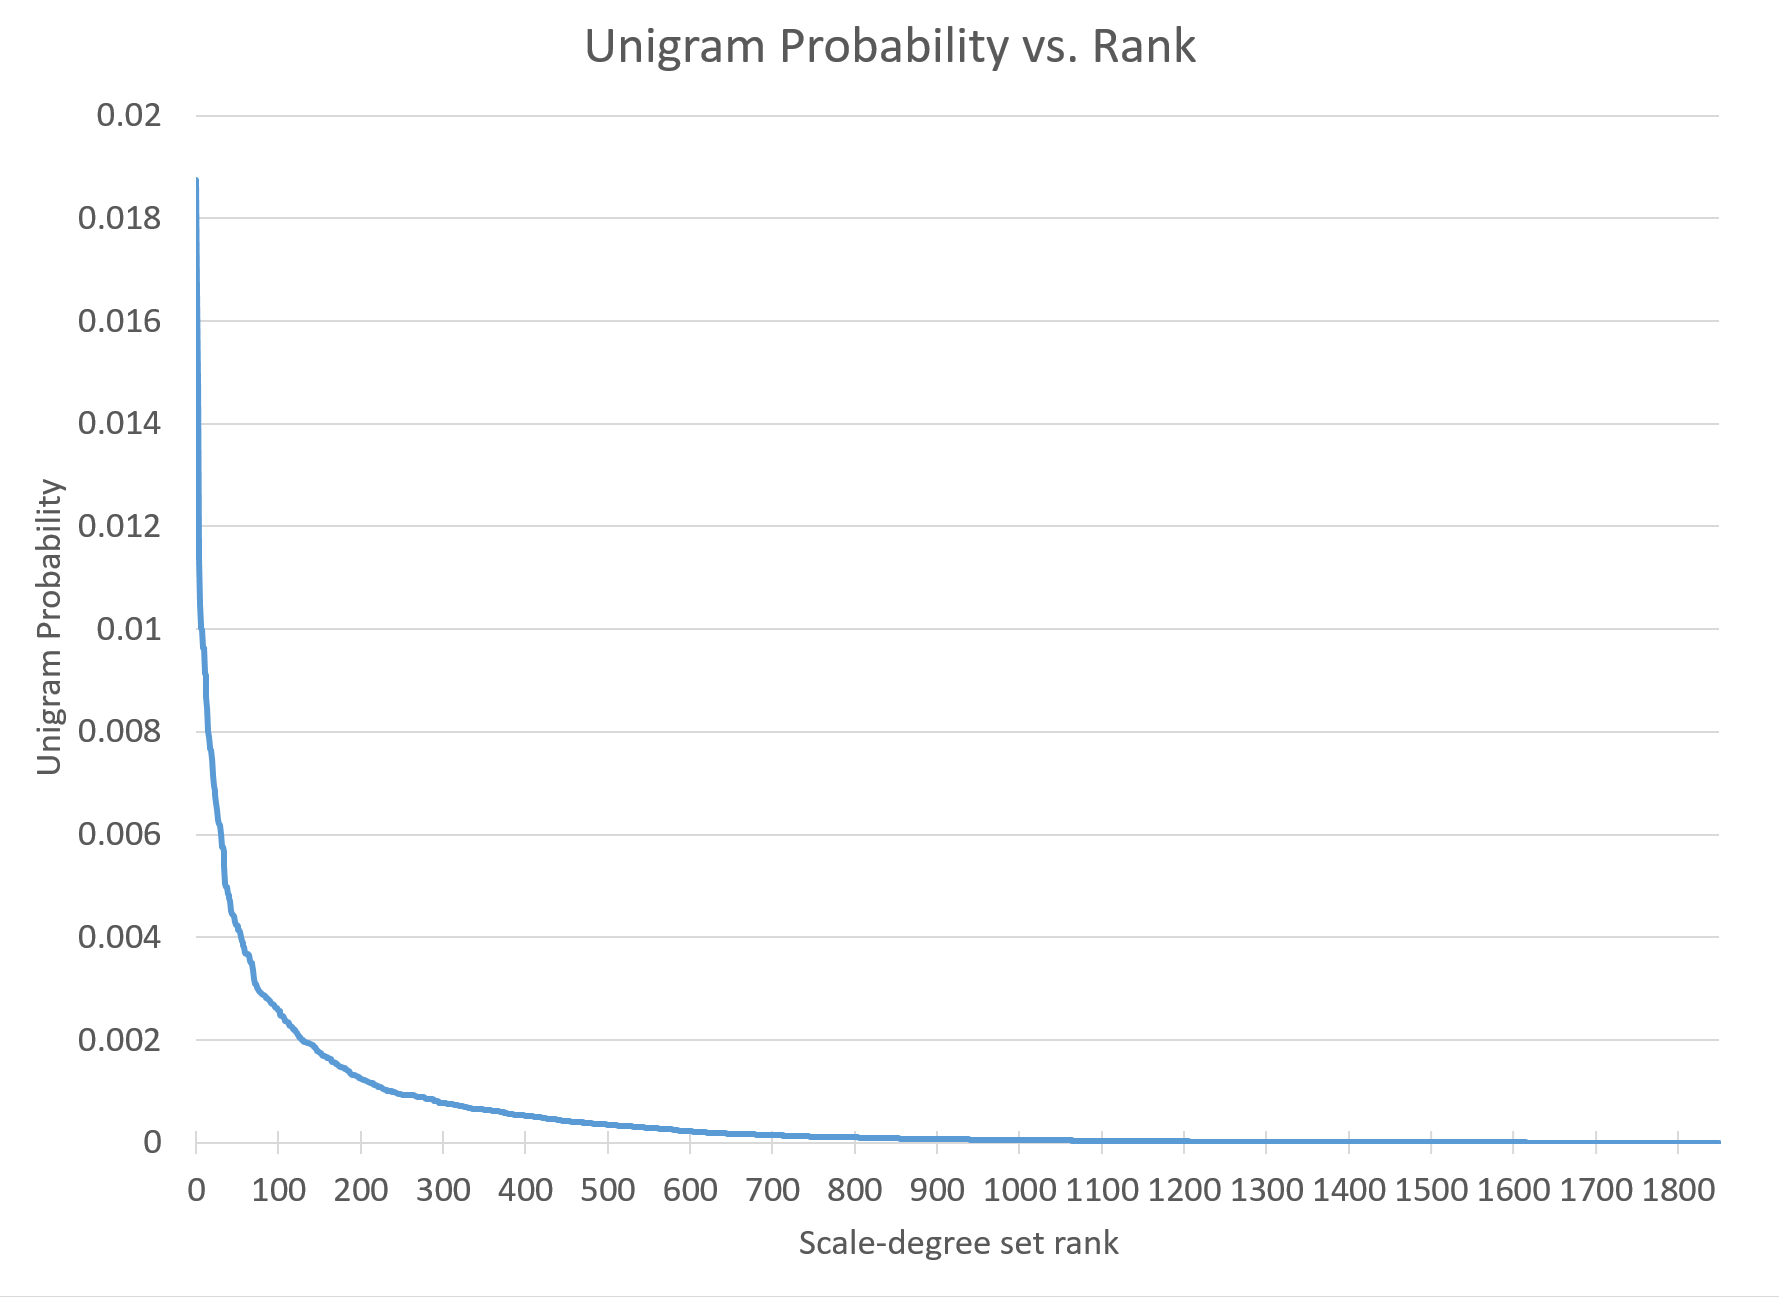
\includegraphics[width=6in]{lexicon_zipfian.png}
	\caption{The unigram probabilities for each of the 1850 distinct scale-degree sets of cardinality three or greater in the YJaMP corpus.  The scale-degree sets are ordered by descending unigram probability.  After around 200 scale-degree sets, the share of overall unigram probability captured by each new marginal set falls below $0.1\%$.}
	\label{lexicon}
\end{figure}

%Truncation and Zipf
Figure~\ref{lexicon} shows the overall unigram distribution for each of the 1850 distinct scale-degree sets of cardinality three or greater.  Like the unigram corpora of many language-like formal systems, it bears resemblance to a Zipfian distribution, where the unigram probability is inversely proportional to each chord's unigram frequency rank.\footnote{Cite some generic Zipf linguistic studies.}  For YJaMP, the distribution of Figure~\ref{lexicon} actually slopes off somewhat more slowly than a true Zipf distribution, with the leftmost part of the curve resembling $\frac{1}{r^s}$ for $0.5 < s < 1$.  For quasi-Zipfian distributions, it is common to truncate the size of the lexicon at some rank indicative of diminishing marginal probability gain. For a na\"{i}ve model consisting of only the most probable chord in the corpus -- that is, a model which predicts that every chord observed ought to be the most common chord in the corpus -- adding a second chord to the model nearly doubles the portion of the corpus data it captures.  Instead of describing the observed chord correctly only 2\% of the time, the model can now describe nearly 4\% of the observations in the corpus.  For a 200 chord model, adding one additional chord only captures at most an additional $0.1\%$.  I deem such an increase in model accuracy unworthy of the substantial increase in complexity.\footnote{Zipfian studies (and corpus-driven models in general) spend considerable time fighting over whether or not given distributions contain ``elbows," where a clear change in the first derivative of the curve signals a justifiable alphabet truncation size.  YJaMP's unigram distribution provides no obvious elbow, but the choice of precise alphabet size is a low-stakes game; choosing a number of chords slightly below or somewhat above 200 changes the ultimate category assignments made by the model by a small amount, and other alphabet size choices are defensible.}

%Manhattan metric and PCA justification
With a 200-chord lexical restriction in place, each origin chord can then be associated with an identically-sized 200 by 100 matrix; the 200 rows correspond to the destination chord probability distributions for the 200 most frequent chords in the corpus, in rank order, and the 100 columns correspond to 100 consecutive 50-millisecond time windows.  For the sake of consistency, ``empty rows" (consisting entirely of zeroes) appear for destination chords which never follow a given origin chord within five seconds.  Identically-sized matrices can be compared element-by-element, dramatically simplifying the construction of similarity metrics.  The Manhattan (or ``Taxicab") distance, a special case of the Minkowski distance metric, sums the difference between corresponding entries in two vectors or arrays.  For vectors $x$ and $y$ with $n$ dimensions each, the Manhattan distance $d_1$ is given by
\begin{eqnarray*}
x &=& (x_1,x_2,...,x_n) \\
y &=& (y_1,y_2,...,y_n) \\
d_1(x,y) &=& \sum_{i=1}^n \lvert x_i - y_i \rvert
\end{eqnarray*}
The ``Manhattan" and ``Taxicab" monikers arise from a common geometric interpretation of this distance: for the case of two-dimensional vectors $x$ and $y$, the metric is exactly analogous to the distance traveled by a taxicab between any two points on the square-block grid of Manhattan.  If no diagonal avenues are allowed, a taxi can only travel along roads which intersect at right angles; accordingly, the driving distance between any two points on the grid can be calculated from the sum of the east-west blocks and north-south blocks separating the origin and destination points.  The Manhattan metric is easily adapted to the matrix comparison task at hand -- each destination chord probability distribution is a 100-dimensional vector, and the Manhattan distance between two such vectors is the sum of the differences between each of their corresponding elements.  If each destination chord vector were viewed as the coordinates of a point in a 100-dimensional geometric space, the resulting Manhattan distance would be the number of ``blocks" traveled by a taxicab moving in one dimension at a time from one point to another.

A na\"{i}ve, element-by-element Manhattan comparison between two temporal probability distribution matrices, however, implies an identical weighting for probability differences in each time window.  While the predictive and functional properties of chords presumably diminish over time, the contributions of background noise and random variation between destination chord distributions will not.  Consider a limiting case, where the temporal probability distributions for destination chords are 1,000-dimensional vectors tracking the appearance of destination chords as late as 50 seconds after a given origin chord.  At times far after an origin chord, the destination chord distributions will almost certainly reflect the background unigram probabilities plus a contribution from small, random fluctuations uncorrelated to a particular origin chord or category.  A Manhattan metric applied to vectors in this high-dimensional space will tally increasing contributions from the random fluctuations, proportionally, drowning out the patterns in phonetic or syntactic progressions at shorter time scales.

%PCA saves the day
Just as it did in Chapter 3, PCA allows the extraction of time scales over which chords experience the highest variance with few assumptions regarding which time scales are too short or too long.  Each origin chord is associated with a matrix of destination chords, and each destination chord is represented by a row of 100 coordinates, each of which indicates the probability of the destination chord's appearance a given number of time windows after the origin chord.  But these 100 coordinates are not the only way to represent the destination chord's probability variance over time.  For each origin chord, running PCA on the set of 100-dimensional destination chords produces a set of principal components, 100-dimensional vectors themselves, capturing the combinations of time windows which account for the greatest amount of variance in the destination chord distributions.  In a way, the principal components provide ready-made templates designed to capture the most common temporal differences between kinds of destination chord behavior.  Destination chord probability distributions can then be written with a much smaller number of coordinates while losing as little accuracy as possible.  Instead of using coordinates to say ``This destination chord appears with 10\% probability at $t=1$, and 5\% probability at $t=2$, and ...", the new coordinate system might be translated to say ``This destination chord's probability curve looks like $1.2$ times the curve given by the first principal component, plus $2$ times the curve given by the second component, plus..."

In this way, each destination chord probability distribution -- each row of the origin chord's associated temporal matrix -- undergoes a basis transformation, a change in its method of coordinate description.  As described in Chapter 3, a PCA algorithm calculates the components themselves by examining coordinate variance across the full set of destination chords of a given matrix, providing one optimized set of principal components per origin chord with which to re-describe them.  And for most origin chords, especially those with high unigram probabilities, the PCA components resemble the phonetic, syntactic, and background components found for $ii$'s destination chords in Chapter 3.

Figure~\ref{PCA_examples} shows four sets of principal components capturing most of the variance in destination chord temporal probability distributions for four different origin chords.  In each case, I have retained the first three principal components.  For nearly all of the 200 most probable chords, three components are enough to capture at least 75\% of the variance in destination chord distributions; in many cases, three components capture more than 90\%.  In each plot of Figure~\ref{PCA_examples}, the components are color-coded in order of descending variance capture: the first component is blue, and typically captures more than 50\% of the variance, while the second and third components are green and red, respectively.  The horizontal axis tracks 50ms time windows, while the vertical axis indicates each component's probability loading per time window.  If an origin chord matrix contained a destination chord with a probability distribution that happened to look exactly like the first principal component, that distribution could be described in this new basis with the coordinates $(1,0,0)$ -- one multiple of the first component, and no contributions from either other component distribution.

%figure: PCA components for 4 top-200 origin chords to explain temporal basis reduction and component alignment
\begin{figure}
	\centering
	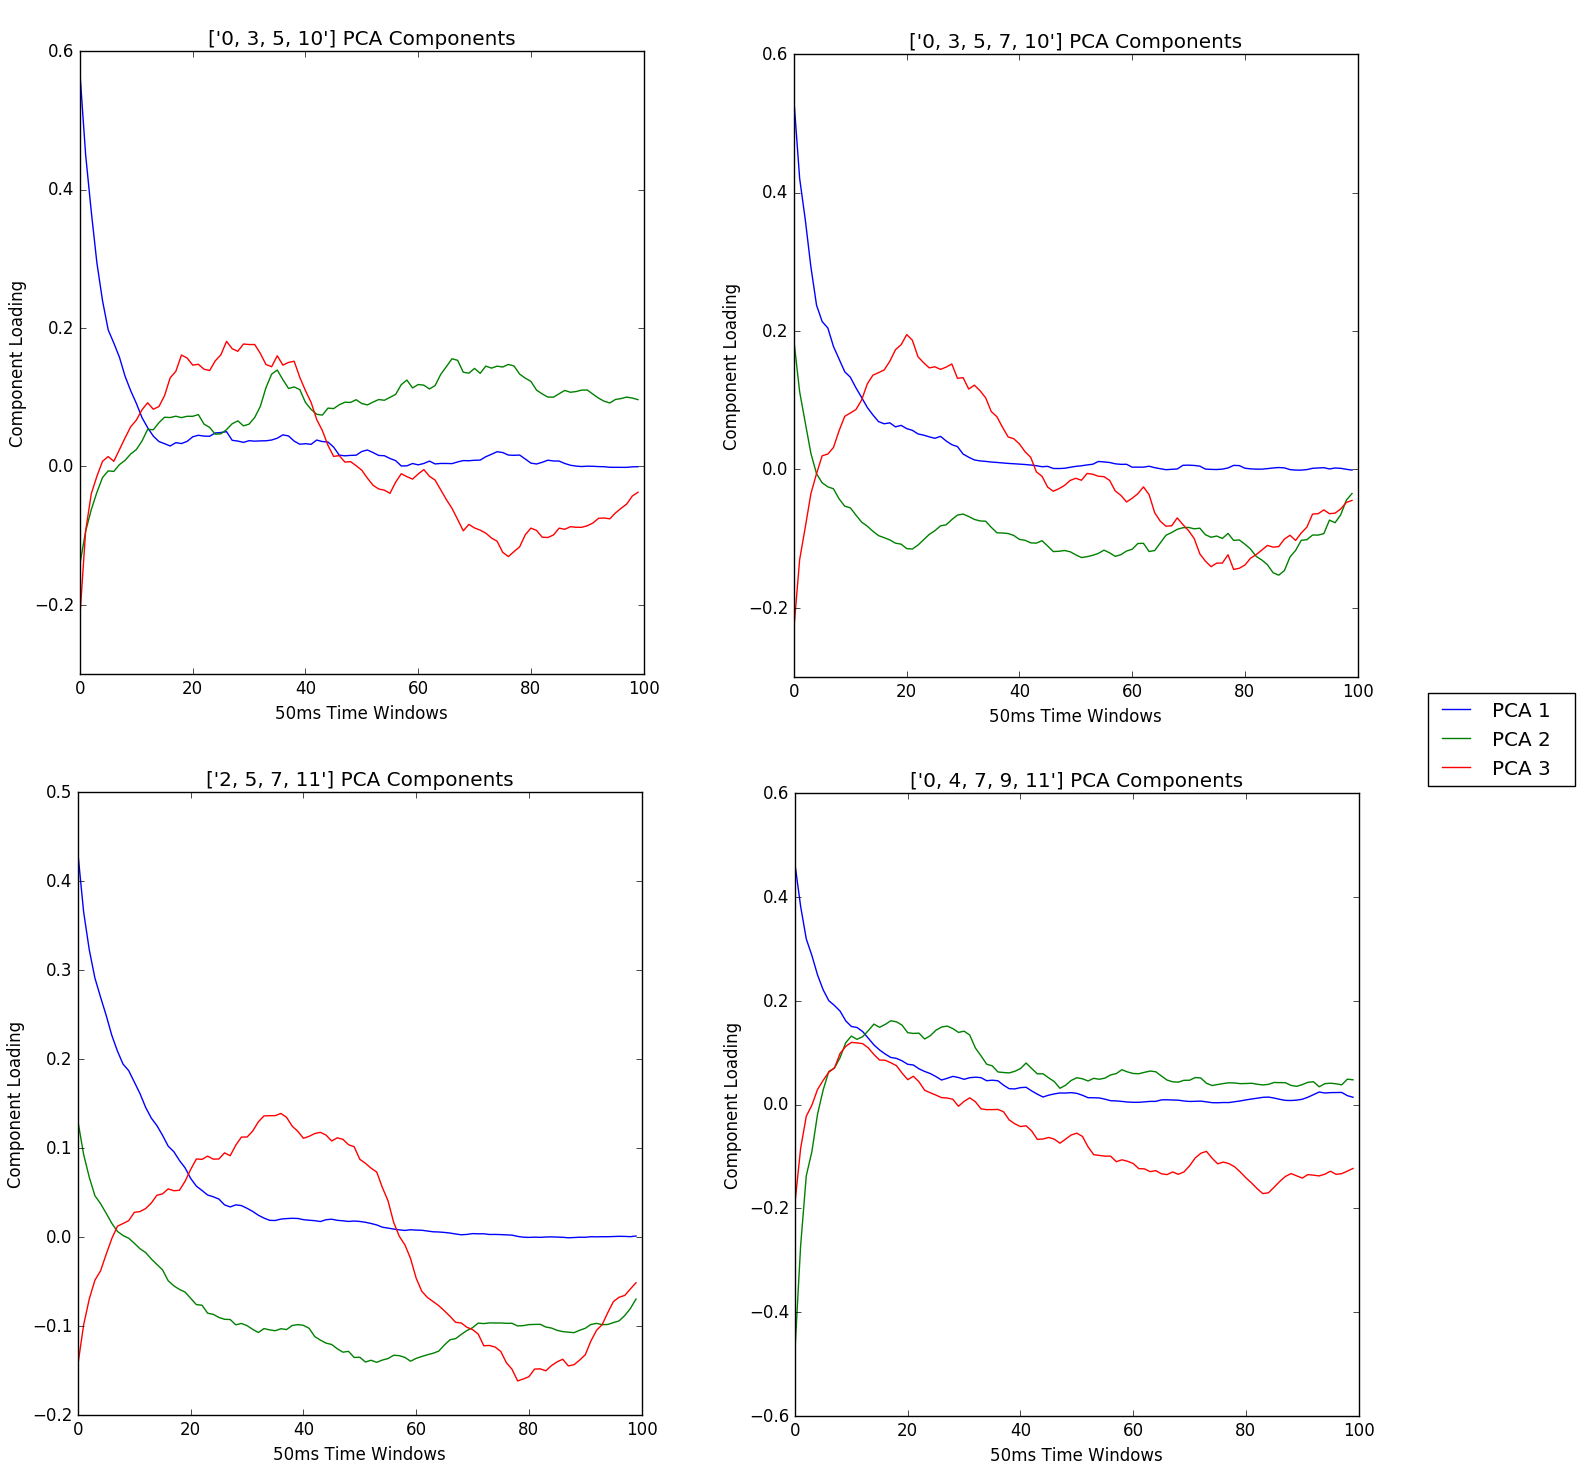
\includegraphics[width=6in]{top200_PCA.png}
	\caption{The first three principal components capturing the most temporal probability variance for four selected origin chords.  For each origin chord, the components provide a three-dimensional reduction of the 100-dimensional destination chord distributions.  Each destination chord's temporal probability distribution can then be written with only three coordinates -- the loadings for each principal component.}
	\label{PCA_examples}
\end{figure}

The top left plot in Figure~\ref{PCA_examples}, calculated from the origin chord $[0,3,5,10]$, shows principal components which directly correspond to the intuitions developed in Chapter 3 regarding temporal progression regimes.  The first (blue) component correlates high initial probability variance shortly after the origin chord with a decrease in variance over time; high coordinate values along this component capture chord behavior characteristic of the phonetic temporal regime, in which origin chords tend to progress to voice-leading neighbor destination chords with similar traditional harmonic functions over short time scales.  Compared to a randomly-chosen destination chord, a phonetic neighbor with a high PCA component 1 score would likely display a large deviation from unigram probability at short time scales, and the deviation in probability would trail off as time after the origin chord increases.  The second (green) component correlates initial probability suppression with a gradual ascent to a stable, non-zero probability value at later times, a combination well-suited to the probabilistic variance of chords common to the local key context but comparatively unlikely to occur as voice-leading neighbors to $[0,3,5,10]$.  The more complex third (red) component implies the most subtle type of temporal progression, yielding a template for destination chords which are suppressed during the phonetic regime but have higher probabilities during a finite time span afterward.  I suggested in the previous chapter that this kind of behavior captures a possible translation of ``syntactic progressions," in traditional theory parlance, where chords unlikely to serve the same local function as the origin chord are more highly probable shortly thereafter than in the long term.  Combinations of these components render the status of many destination chords ambiguous, but this simplified explanation serves to indicate the connection between principal components and destination chord probability distributions in broad strokes.

The components for the other origin chords of Figure~\ref{PCA_examples} serve to block over-interpretation of the salient features of $[0,3,5,10]$.  In each case, component one matches phonetic-scale probability expectations, but one or both of the other components appear quite different.  The nature of this difference arises from PCA itself.  If each component provides a new basis direction along which destination chords are likely to show great variance, the orientation of any particular destination chord's variance along that direction is not reflected in the principal component.  Each component captures not just one kind of probabilistic behavior, but \emph{two}: if a destination chord distribution exactly resembling the first component can be assigned PCA-basis coordinates $(1,0,0)$, a destination chord distribution showing exactly the opposite behavior -- strongly suppressed at short distances, asymptotically increasing over long durations -- could be captured by the coordinates $(-1,0,0)$.  The same component would exactly capture the probability fluctuations of the destination chord, but the relevant coordinate would carry a negative sign.

Figure~\ref{PCA_examples} thus serves as an encoded set of instructions for how to find particular kinds of chords.  To find destination chords after $[0,3,5,10]$ matching intuitive expectations for phonetic, background, and syntactic-regime progressions, the analyst should examine chords with high, positive coordinate scores along each of the three principal components.  For $[0,3,5,7,10]$, the PCA components for which appear in the top right portion of Figure~\ref{PCA_examples}, the same is true up to a correction of sign: destination chords with phonetic and syntactic regime behavior will be written with high, positive coordinates along PCA components one and three, but background-type destination chords will be written with \emph{negative} scores along the direction of PCA component two.  In other words, component two for $[0,3,5,7,10]$ resembles the mirror image of component two for $[0,3,5,10]$, its multiple by negative one, so background destination chords with positive coordinates along component two for $[0,3,5,10]$ will have similar probability distributions to destination chords with negative components along component two for $[0,3,5,7,10]$.  The same sign change describes the component difference for the bottom-left plot of Figure~\ref{PCA_examples}, $[2,5,7,11]$; like $[0,3,5,7,10]$, its second component resembles the mirror image (or negative multiple) of the second component of $[0,3,5,10]$.

The bottom-right plot, $[0,4,7,9,11]$, displays components with similar contours to the other three plots, but on a compressed time-scale.  The rate of decrease in component one and initial increases for components two and three occur much closer to the origin chord than the corresponding components for the other plotted origin chords.  This likely reflects the decreased predictive power of a tonic chord.  Within a few time windows after the appearance of $[0,4,7,9,11]$, component one indicates that voice-leading neighbors still occur with greatly increased probability, but the overall probability variance after 20 windows or so is quite small.  This provides a graphical translation of received harmonic wisdom: the appearance of a $I$ or $vi$ chord tells the analyst very little about what chords likely appear in the future, as nearly any key-appropriate chord can follow tonic chords in a syntactic phrase.

The principal components for a large number of the top 200 most probable chords in the YJaMP corpus afford observations of this nature to such an extent that the intuitive interpretation of basis components can be standardized and automated.  To see if a destination chord shows the same kind of probability fluctuations after two different origin chords, an algorithm can compare the destination chord's PCA-basis coordinates up to an overall alignment of signs.  A metric comparing two origin chord matrices, then, needs only to align the corresponding PCA components by multiplying one or more columns by negative one to achieve an imposed, standard alignment: component one starts with positive value, and components two and three start with negative values.  This alignment is arbitrary, but the resulting standardization comes at no real cost.

As a result, I compare origin chords by imposing a Manhattan metric on matrices consisting of the destination chord temporal probability distributions for the 200 most probable chords in the corpus written in a systematically-aligned, PCA-reduced basis.  Each origin chord corresponds to a matrix with 200 rows and three columns, and I employ a dissimilarity ``distance" between two origin chords defined as the sum of the absolute differences between corresponding elements in their respective matrices.  In more formal notation, the distance $d$ between chords $\alpha$ and $\beta$ is given by

\begin{equation}
d(\alpha, \beta) = \sum_{i=1}^{200} \sum_{j=1}^3 \lvert \alpha_{ij} - \beta_{ij} \rvert
\end{equation}

This distance metric remains agnostic about the pitch structures of the origin and destination chords, and it provides a (dis)similarity metric based purely on progression statistics; a larger Manhattan distance $d$ between two matrices $\alpha$ and $\beta$ correlates with a sense of increased difference between the progression behavior of the corresponding origin chords.  As the next section will show, a metric of this kind allows clustering algorithms to group origin chords together based on similarity in their overall progression tendencies, yielding a rough approximation of chord categories assembled from behavioral statistics.

\section{Clustering methods}
%with Manhattan metric in hand, explain at least flat agglomerative clustering for (functional?) categories
%go into detail about agglomerative hierarchical clustering on the topN-filtered, PCA-transformed matrices
Clustering algorithms, in their simplest form, pursue a single goal: given an array of objects described in some coordinate basis, group the objects into categories where the members of each category are ``closer" (or ``more similar") to one another than they are to members of the other categories.  Aside from the input objects, described with some consistent representation scheme, most clustering algorithms require the analyst to supply two further input choices -- a similarity metric for comparing objects to one another, and a way to determine the boundaries of each cluster.  If the input objects are represented in a basis that lends itself to a geometric interpretation (like spatial coordinates), the process of drawing these cluster boundaries may be interpreted as outlining shapes or surfaces containing the objects.  The resulting points in each category would be found close to one another, geometrically speaking -- ``clustered" together.

%hierarchical clustering in general; greedy algorithms
Hierarchical clustering algorithms approach the very complex problem of how to partition a large number of data points into clusters by splitting it into a series of simpler problems.  Starting from either of two limiting cases -- either there is only one giant cluster, into which all data points fall, or every point is its own cluster -- hierarchical clustering first either splits the giant cluster into two smaller clusters (the former, ``divisive" clustering case) or merges an individual point cluster with its closest metric-determined neighbor (the latter, ``agglomerative"  method).  As a result, the algorithm replaces the na\"{i}ve limiting case with a slightly more nuanced approximate clustering.  Repeating the split or merge step many times, hierarchical clustering gradually produces an approximation of the optimal clustering.  For each step, hierarchical clustering algorithms perform what computer scientists refer to as ``greedy" optimization, using all available dissimilarity information provided by the metric to make the best possible local decision without any consideration of its future effects; strict hierarchical clustering makes no attempt to guess in advance what cluster assignments many successive splits/merges will produce.  Due to their computationally efficient short-sightedness, greedy hierarchical clustering algorithms can occasionally get off track, producing final clusterings which poorly capture the intuitive structure of the data.

%bad results from divisive clustering?  Agglom works well; explain it
With no method for planning the end results of the greedy optimization, divisive hierarchical clustering algorithms start with a trickier task than agglomerative ones: there are many possible ways to split a large data set into two clusters, and the immediate differences between initial splits may be small.  For a noisy data set, however, many initially-productive splittings can turn out to produce ill effects in the final clustering, as data points comparatively close together might be placed into different clusters early on to optimize cluster-level criteria.  Agglomerative hierarchical clustering approaches the problem from the opposite direction.  If divisive clustering is a ``top-down" process, requiring a heuristic for how to split clusters most effectively, agglomerative clustering is a ``bottom-up" procedure, where each merge step uses the metric to determine which points 9or groups of points) are closest together.  Closely-related objects are less likely to end up placed far apart, but another kind of judgment call is still required: a linkage criterion indicating how to calculate the distance between a single data point and a cluster of arbitrary size.  If a merge operation places a point (or many points) into a cluster, it must evaluate which cluster would be the best, ``closest" assignment.  Several ways of specifying this linkage criterion are possible, but ``complete" or ``maximum" linkage provides the best results for clustering the YJaMP temporal probability matrices.\footnote{Two types of sub-optimal behavior accrue as a result of other linkage criteria: either category assignments violate a large number of syntactic expectations, or the resulting clusters differ radically in size -- one cluster might have 100 origin chords, and a dozen other clusters might contain a handful of chords each.}

Maximum linkage describes inter-cluster distance as the \emph{largest} distance between any two points in the respective clusters.  Put formally, the distance between two chord clusters $A$ and $B$ ($d_l$) can be calculated from the Manhattan-metric distances ($d_m$) between the chords in each cluster:
\begin{equation}
\label{eq:d_l}
d_l(A,B) = \max \{ d_m(c_1,c_2) \vert c_1 \in A, c_2 \in B \}
\end{equation}
Each merge step adds a single point to a cluster or combines two clusters in order to optimize the linkage criteria $d_l$.  After many such merge steps, agglomerative hierarchical clustering produces cluster assignments for the full range of observations -- in YJaMP's case, the top 200 most probable origin chords.

%now describe the results
%First, what the dendrogram even means
Running agglomerative hierarchical clustering of this kind with the sklearn (``scikit-learn") Python package produces the dendrogram given in Figure~\ref{Dend_complete}.  The 200 most unigram-probable chords are listed at the bottom of the figure in an order automatically chosen to keep cluster members adjacent to their nearest neighbors.  Each bracket on the dendrogram represents a merge operation, and the vertical-axis height of each bracket reflects the distance between its two associated ``children."  At the bottom of the figure, origin chords connected by a bracket constitute merges which associate a single chord (or ``leaf," in dendrogram parlance) with the chord deemed most similar to it -- that is, with the chord which minimizes $d_l$ in Equation~\ref{eq:d_l} above.  Higher up in the ``tree," branchings indicate merge steps where at least one of the clusters contains multiple chords.  Hierarchical clustering provides multiple levels of similarity ranging from point-to-point up to broad cluster-to-cluster comparisons.  In YJaMP's terms, this range of groupings indexes both similarity between individual chords (near the bottom of the tree) and a functional or modal organization of the origin chords into a small number of categories (near the top of the tree).

The color coded portion of the tree in Figure~\ref{Dend_complete} provides rough category assignments for the clusters.  The decision where to ``cut" the dendrogram into large-scale category clusters is comparatively arbitrary, and I impose it here via the Python package SciPy's \emph{fcluster} function, which color codes clusters based on a supplied inter-cluster distance, a particular choice of vertical-axis inter-cluster distance at which to identify categories.  I set that threshold high enough reduce the number of clusters as much as possible while minimizing the extent to which clusters containing functionally-different chords are merged.  As this is a heuristic decision, other choices of cut point are clearly defensible, and imposing them merely requires modifying the color-coding on Figure~\ref{Dend_complete}, choosing instead to categorize clusters at a slightly higher or lower location on the dendrogram.  As it stands, Figure~\ref{Dend_complete} color codes 59 potential clusters, 28 of which contain more than one chord.  The full dendrogram is difficult to read, so a series of subplots appear below.

%the big agglom clus dendrogram, at least three subplots thereof with annotation and explanation
\begin{figure}
	\centering
	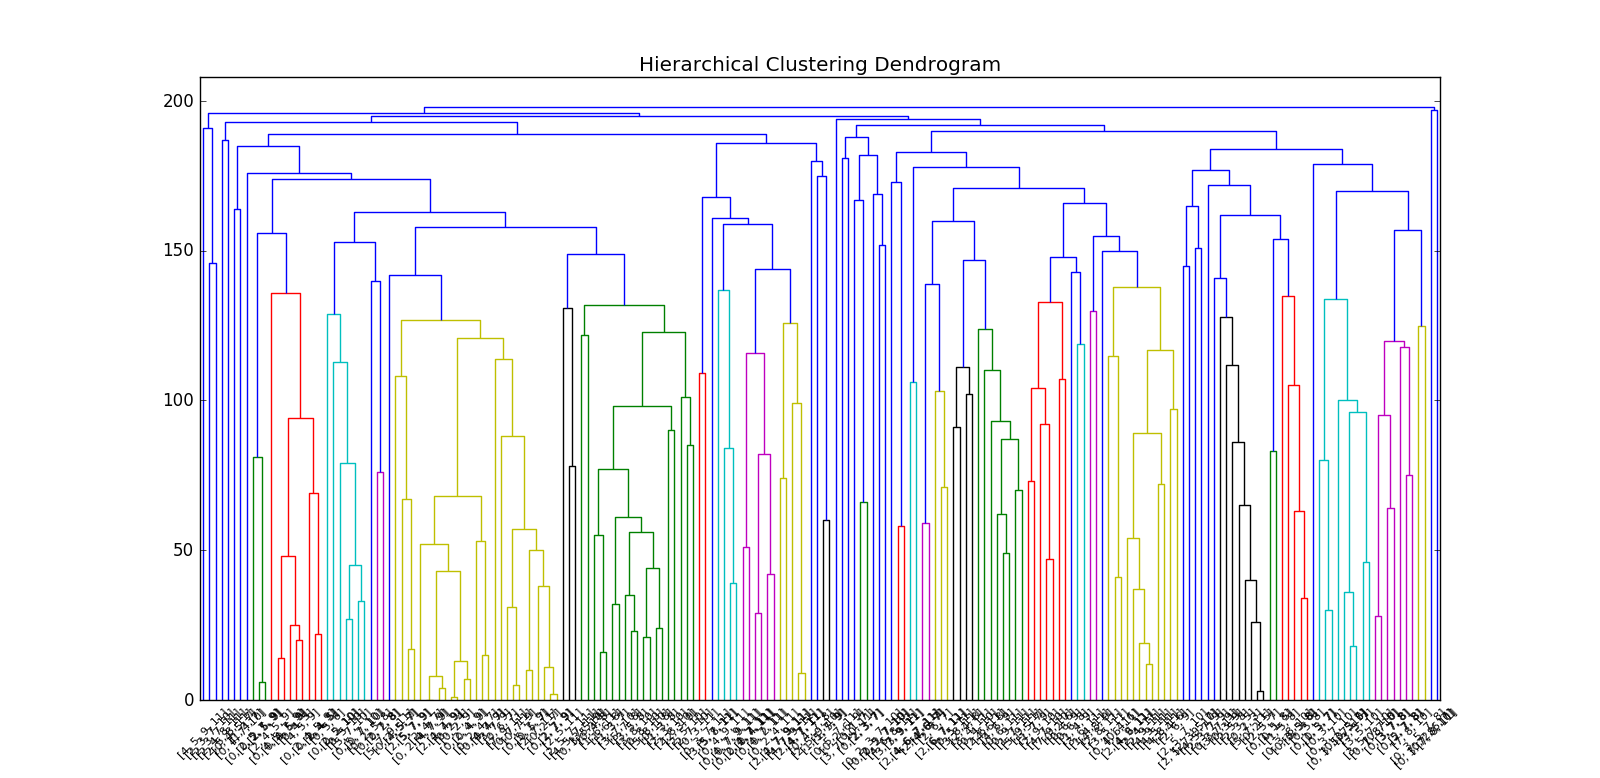
\includegraphics[width=6in]{Dendrogram_complete.png}
	\caption{The full dendrogram for agglomerative hierarchical clustering of the top 200 most frequent chords in the YJaMP corpus.  Chord-to-chord distances (or dissimilarities) are calculated from PCA-reduced temporal probability distribution matrices for each chord.}
	\label{Dend_complete}
\end{figure}

Figure~\ref{Dend_sub1} shows several chord clusters capturing pre-existing harmonic expectations for normative jazz substitutions.  At left, the green and red clusters contain scale degree sets readily interpretable as varieties of $ii$ and $IV$ triads, seventh chords, and their tonally-appropriate supersets.  The green cluster groups $[2,5,9]$, the $ii$ triad in a local key, with $[0,2,5,9]$, a fully-voiced $ii^7$, and $[0,2,5,7,9]$, which could be interpreted as a $ii^{7}$ with an added 11th.  The adjacency of these three scale degree sets in the dendrogram indicates close similarity in their progression matrices, and the shortest brackets, like the one connecting $[2,5,9]$ and $[0,2,5,9]$, correspond to the closest merges.  The red cluster contains $[0,4,5,9]$, a fully-voiced $IV^7$ in the local key, as well as $[4,5,9]$, a root-third-seventh $IV^7$ voicing, and $[0,5,9]$, the $IV$ triad.  But it also captures scale-degree sets we might describe as ambiguously-rooted $ii-IV$ blends, like $[0,2,4,5,9]$, or as related scale segments, like $[2,4,5,9]$ and $[0,2,4,5]$.\footnote{Both of the latter examples, like all the scale-degree sets on the dendrogram, might be voiced in a variety of ways, so interpretive caution is advised.  If $[0,2,4,5]$ were voiced in the smallest possible span (say, $[C4,D4,E4,F4]$) it would indeed resemble a scale segment -- but if it were instead voiced as $[D4,F4,C5,E5]$, an analyst might label it as a $ii^9$ chord.}   Here, we might interpret the red and green clusters as predominant or subdominant functions, and we can see from Figure~\ref{Dend_complete} that the merge operation one level above the color coding of each of these clusters groups them together; the red and green clusters are more similar to each other than they are to the other clusters produced by the agglomerative algorithm.

At the far right of Figure~\ref{Dend_sub1}, black brackets delineate a cluster quite different from the red or green clusters.  Here, dominant-function scale-degree sets appear in proximity to one another, including $[2,5,11]$, the $vii^{\circ}$ triad, $[2,5,7,11]$, a fully-voiced $V^7$ chord, and $[4,5,7,11]$, which might be identified as a $V^7$ chord with an added 13.  This comparatively small cluster consists of chords with a rather constrained syntactic function.  In contrast, the large yellow cluster in the middle of Figure~\ref{Dend_sub1} contains major-key ``tonic" type chords and scale segments, broadly construed.  It includes tonic representatives of $iii$ ($[2,4,7]$), $vi$ ([$0,4,9]$ and $[0,4,7,9]$), and $I$ ($[0,4,7]$).  The function of each individual chord in the yellow cluster is harder to pin down (what is a $[4,5,7]$ chord?), but the members of the cluster have progression statistics more similar to one another -- and to major tonics without a leading tone in them -- than to members of other clusters.

On the smallest scale, the agglomerative clustering describes $[0,4,7]$ and $[0,4,7,9]$ as closest-neighbors.  This reproduces an old jazz-analytical truism regarding stable tonics, but it does so in a way which avoids the usual complications of roman numeral analysis.  Jazz texts written by Mehegan, Levine, Terefenko, and others describe $[0,4,7,9]$ as either a $VI^7$ chord or as a $I^6$ chord, depending on its inversional voicing; with a $\hat{6}$ in the bass, the sonority tends to receive the former roman numeral, while a chord featuring $\hat{6}$ in the top voice receives the latter.  The agglomerative clustering of Figure~\ref{Dend_sub1} knows nothing about the ``root ambiguity" of $[0,4,7,9]$ -- nor does it know that the chord shares three of its scale degrees with $[0,4,7]$.  The clustering places them adjacent to one another because their temporal progression statistics are extremely similar -- they ``behave" the same way.  This tonic ``way of behaving" can evidently be expanded to instances of $[2,7,11]$, the dissonance-free $V$ triad, and various diatonic scale segments. 

\begin{figure}
	\centering
	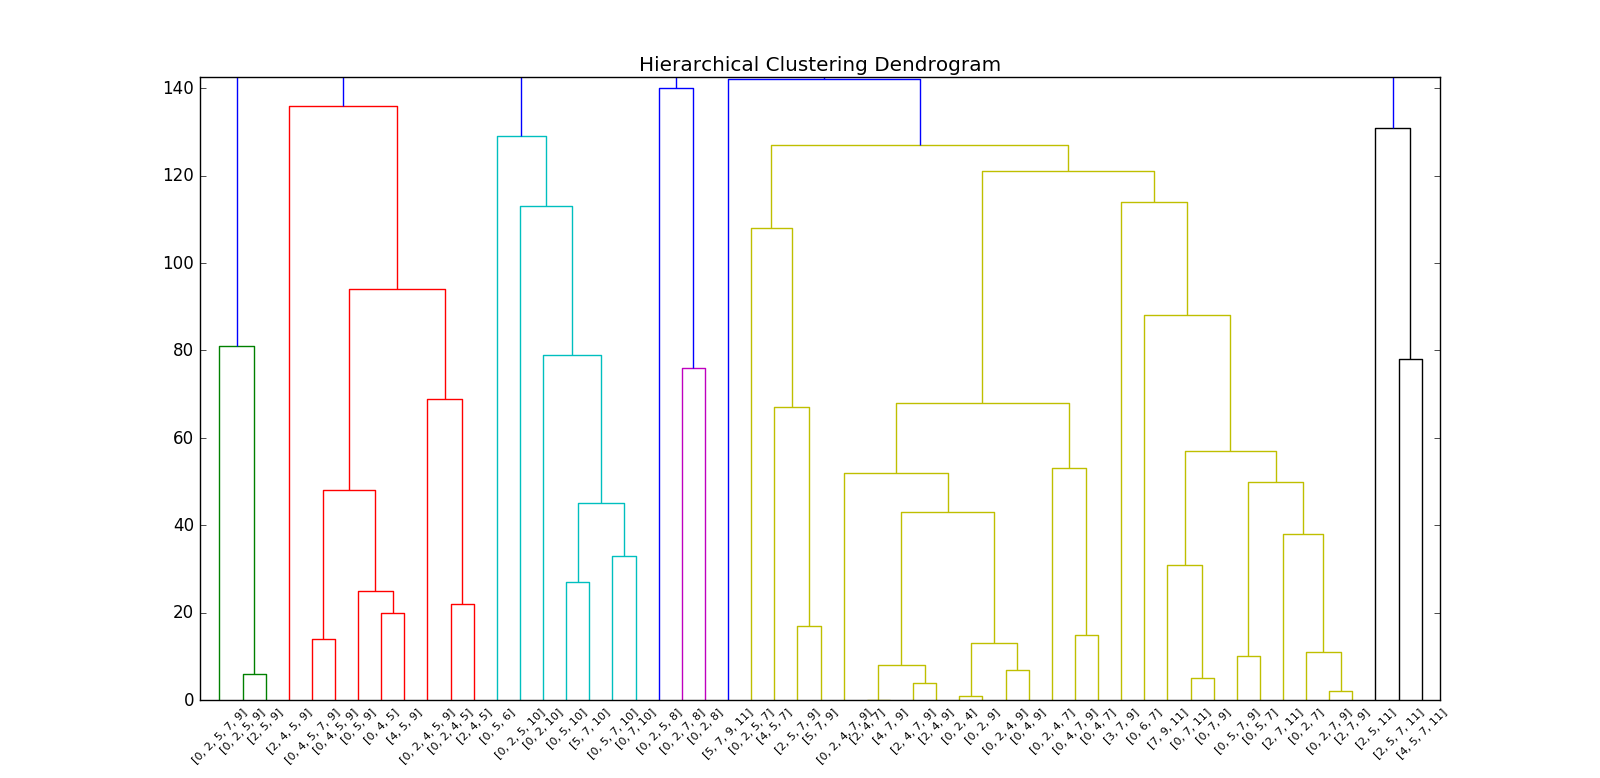
\includegraphics[width=6in]{Dend_ii_IV_I_vi_V.png}
	\caption{Close-up of Figure~\ref{Dend_complete}.  Color-coded clusters here capture categories corresponding to traditional scale degree set descriptions of $ii$, $IV$, $I$, $vi$, and $V$.  Note that the clustering algorithm knows only the behavior of the chords -- not their pitch class content.}
	\label{Dend_sub1}
\end{figure}
%iv appears in both of the below.  Is this because iv behaves differently in major vs. minor key contexts?
\begin{figure}
	\centering
	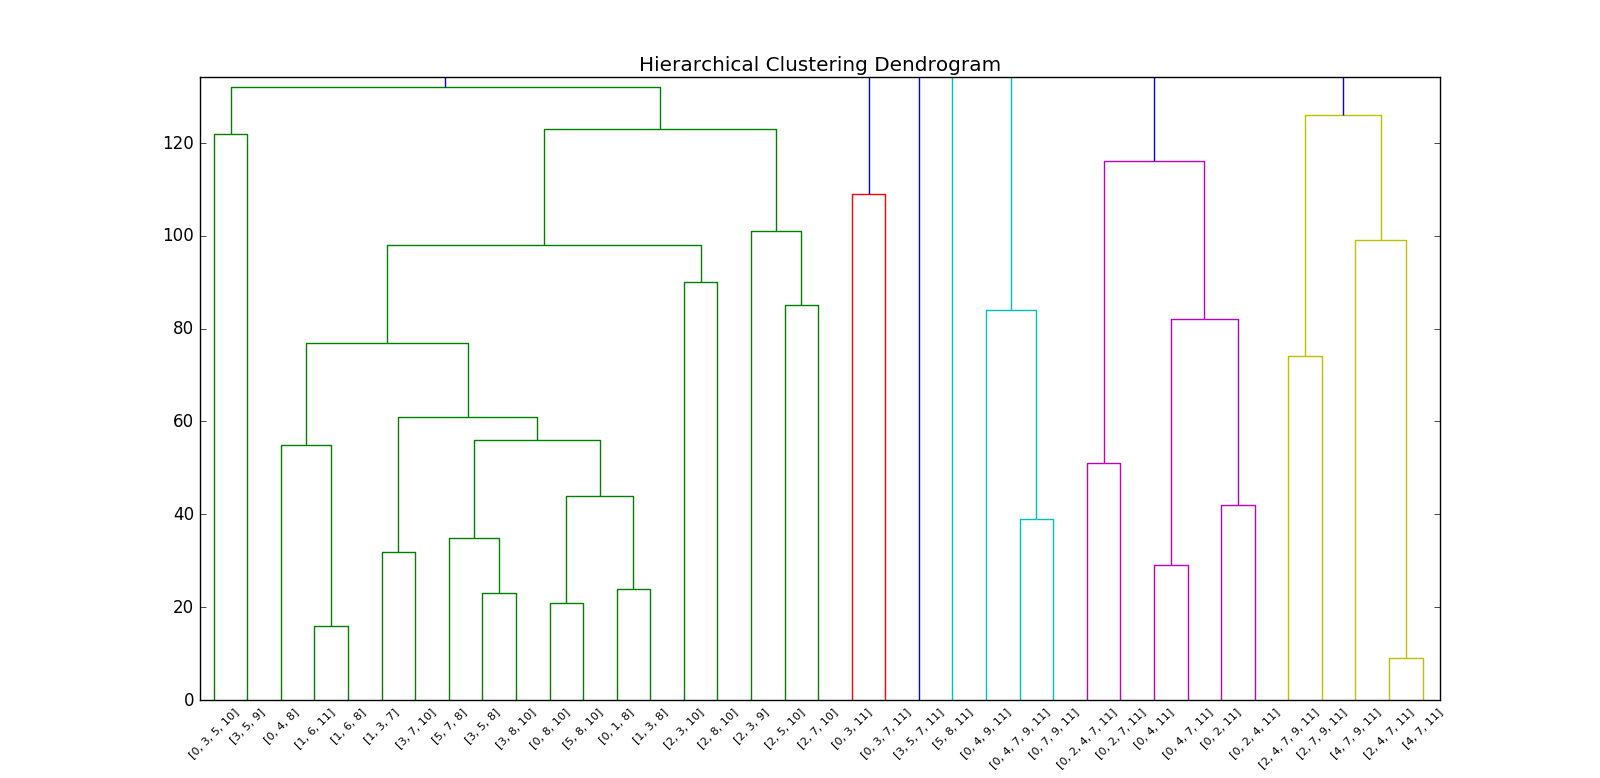
\includegraphics[width=6in]{Dend_iv_I7_iii.png}
	\caption{Close-up of Figure~\ref{Dend_complete}.  Color-coded clusters here capture categories corresponding to traditional scale degree set descriptions of $iv$, $I^7$, and $iii$.  Note that the clustering algorithm knows only the behavior of the chords -- not their pitch class content.}
	\label{Dend_sub2}
\end{figure}

Figure~\ref{Dend_sub2} contains a similar range of functional clusters.  At right are several clusters containing the leading tone ($[11]$ or $\hat{7}$).  The yellow cluster contains varieties of $iii^7$, like $[2,4,7,11]$ and $[4,7,11]$, as well as pitch class sets we might describe as root-ambiguous, or both $V$-like and $iii$-like.  The agglomerative clustering here sidesteps whether $[2,4,7,9,11]$ should be described as a $V$ triad with added sixth and ninth (less likely, due to the missing chordal seventh, but logically permissible) or as a $iii^{11}$; of importance to the clustering is that the scale-degree set behaves in a way very similar to the other chords in the cluster, several of which resemble traditional $iii$ chords.  The purple and cyan clusters on the right hand side of Figure~\ref{Dend_sub2} also contain tonic-type chords.  The majority of the purple curve consists of $I^7$ voicings, while the chords of the cyan cluster typically feature the addition of $\hat{6}$ (i.e., the purple cluster contains $[0,4,7,11]$, while the cyan cluster contains $[0,4,7,9,11]$).  Both the purple and cyan clusters separate the voice-leading behavior of major tonics containing leading tones from Figure~\ref{Dend_sub1}'s cluster of leading-tone-free tonics, and all three of the of the clusters at right on Figure~\ref{Dend_sub2} are similar enough to merge at the next branching point up the hierarchical tree.

Figure~\ref{Dend_sub3} shows a variety clusters suggestive of minor keys and ``flat-side" harmony.  In the cyan cluster near the middle, $[0,3,7]$, $[0,3,10]$, and $[0,3,7,10]$ appear adjacent to one another -- the three most common scale-degree expressions of the minor tonic chord.  The remainder of the cyan cluster indicates that the addition of scale degree $\hat{4}$ (in chromatic semitonal notation, $[5]$) to minor tonic chords leaves their progression statistics relatively unchanged.  While $[0,3,7]$, $[0,3,10]$, and $[0,3,7,10]$ fall in the left cyan ``subcluster," $[0,3,5,7]$, $[3,5,10]$, and $[0,3,5,7,10]$ all fall in the right.  This clustering appears to support the ``extended harmony" dictum that perfect 11ths may be added to minor chords without significantly altering their functional properties.  The purple cluster to the right contains many instances of minor tonic scale degrees $\hat{1}$, $\flat\hat{3}$, $\hat{5}$, and $\flat\hat{7}$ ($[0,3,7,$ and $10]$), but with the frequent addition of $\flat\hat{6}$ ($[8]$).  This includes chords that might carry roman numeral label $\flat VI$, like $[0,7,8]$ and $[0,3,7,8]$, as well as more ambiguous collections of minor key scale degrees, like $[7,8,10]$ and $[2,7,8]$.  This cluster's composition does not necessarily indicate that the chords appear exclusively in minor keys; rather, it demonstrates that they progress the same way over time, whether as modal mixture in major key contexts, flat-side modulatory passages, or as diatonic minor harmonies.

%Weird clusters
Aside from recognizably predominant, dominant, and tonic clusters in major and minor modes, the agglomerative clustering of Figure~\ref{Dend_complete} provides both a framework for categorizing systematically-used chords of lower probability and an indication of where the limits of cluster interpretation might lie.  The cyan cluster on the left hand side of Figure~\ref{Dend_sub1} contains a collection of chords bearing family resemblance, where no single scale degree or root occurs across all members of the cluster.  Most of the chords contain scale degree $\flat\hat{7}$, whether as part of a $v$ (like $[5,7,10]$) or a scale-degree set potentially identifiable as $\flat VII$ (like $[0,2,5,10]$), and each chord contains at least two scale degrees in common with its nearest neighbors.

%Green cluster of Figure~\ref{Dend_sub2}.  Has a lot of [8] in it?  Some bVII and v?  Possible junk drawer?
The green cluster at the left hand side of Figure~\ref{Dend_sub2} elevates the ambiguity of traditional interpretation to levels which cast doubt on the utility of the cluster.  Here, scale degree sets corresponding to $v$ ($[2,7,10]$) and $\flat VII$ ($[2,5,10]$) share a large cluster with root-third-seventh voicings $[3,5,8]$ and $[3,5,9]$.  The latter might be interpreted as a $V^7 / \flat VII$, and several other flat-side chords relative to that key area also appear (like $[3,7,10]$), but the cluster otherwise bears some resemblance to a ``junk drawer," a cluster into which the algorithm dumps noisy chords with complex behavior.

None of the chords in this green cluster are among the top 100 most unigram-probable chords except $[2,7,10]$, $[2,5,10]$, $[3,5,8]$, and $[3,7,10]$, a fact which reflects the increasing difficulty of clustering lower-probability chords in an intuitively (or syntactically) meaningful way.  When the agglomerative hierarchical clustering algorithm is given a large number of low-probability chords to tag with cluster labels, the perceived syntactic consistency of the clusters begins to break down.  Under such conditions, investigations into the potential behavior of low-probability chords benefit from \emph{supervised} machine learning classifier methods, where the initial clustering of high-probability chords is taken as a given, and new chords are categorized with respect to the initial framework. 

\begin{figure}
	\centering
	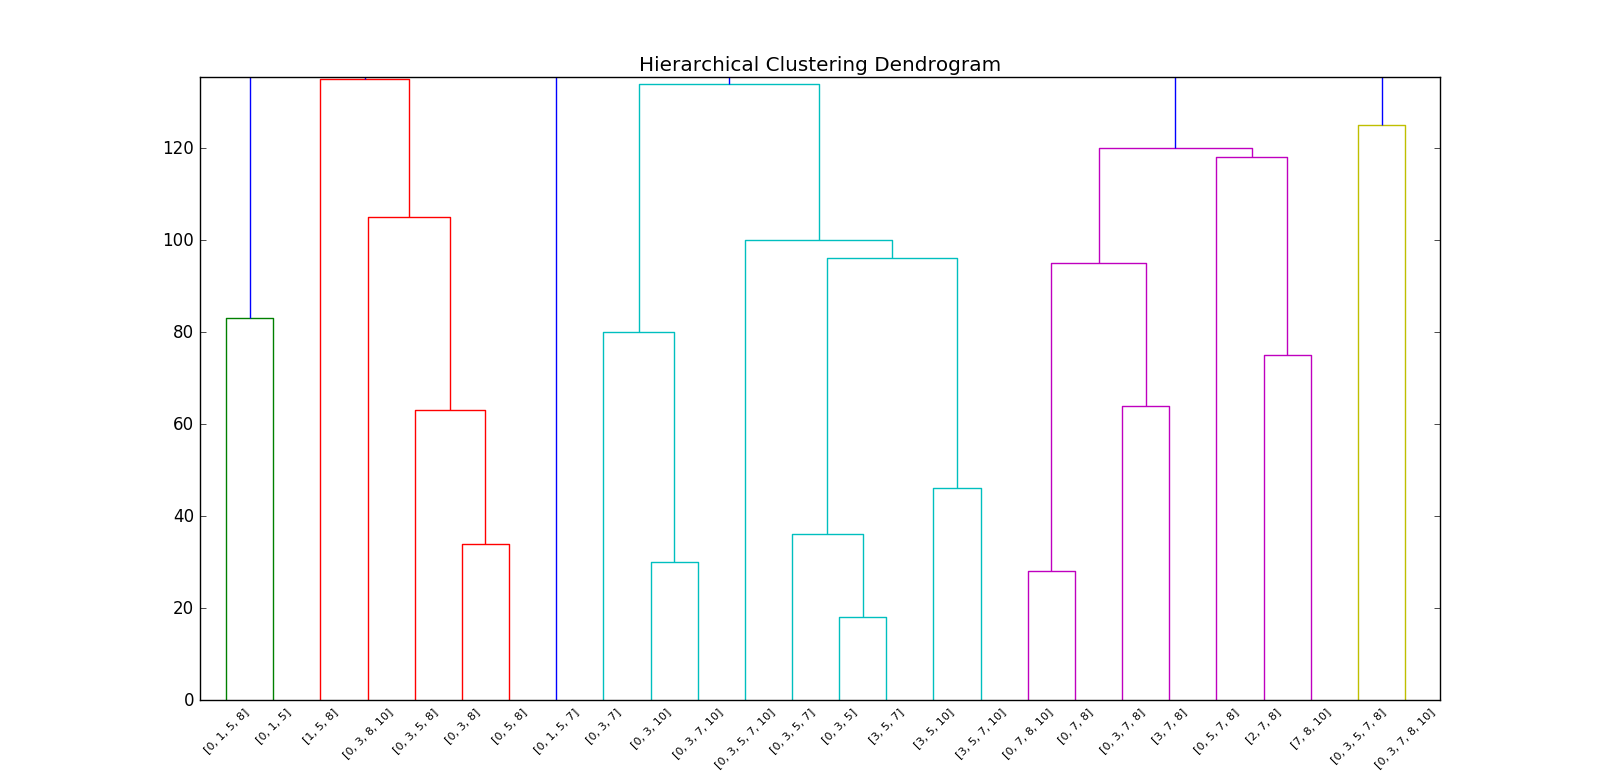
\includegraphics[width=6in]{Dend_iv_bVI_i.png}
	\caption{Close-up of Figure~\ref{Dend_complete}.  Color-coded clusters here capture categories corresponding to traditional scale degree set descriptions of $iv$, $\flat VI$, and $i$.  Note that the clustering algorithm knows only the behavior of the chords -- not their pitch class content.}
	\label{Dend_sub3}
\end{figure}

\section{Generalized harmonic syntax: categories and classifications}
%Lay out the general problem: want to get categories without noise -- especially so we can see useful behavior -- but then also use those categories for classifying noisier states
%Note that various types of machine learning algorithm can place lower-P chords into the flat agglomerative clustering classes; don't come down on one firm algorithm.
%MAYBE: Then note that training on high-P chords allows us to see some of what categories "do" (cat-to-cat transitions?)
Given a set of meaningful category assignments for high-probability chords, as introduced in the previous section, lower-probability chords may be classified into these categories by machine learning algorithms trained on the set of high-probability category assignments.  Supervised machine learning algorithms take a predictive stance with respect to ``new" observations, using patterns gleaned from known classifications to guess what tag should be assigned to a previously unseen observation.  Different specific algorithms accomplish the task in different ways, but each ``learns" from a training set -- high-probability chords and their cluster assignments, in this case -- and then attempts to extrapolate that learning to make predictions about sensible class assignments for elements of a testing set -- here, lower-probability chords not captured by the initial clustering.

Two important kinds of optimization confront any analyst choosing from the wide variety of supervised classifiers.  First, the value of a given classifier is typically assessed by examining how well it performs on a subset of the data for which the desired category assignments are known.\footnote{Give a source for cross-validation?}  In the case of YJaMP's syntactic clustering, this cross-validation scheme involves separating the flat clustering itself, in which all of the 200 most probable chords receive cluster assignments, into distinct training and testing sets.  If a machine learning algorithm is trained on a random selection of 80\% of the top 200 chords, comparing their temporal probability matrices to their cluster assignments in order to generate a predictive model mapping the former to the latter, it can then be tested on the remaining 20\% , chords which the model has never seen.  Since the flat clustering provides category assignments for these chords -- assignments the machine learning model did not see or use in its predictions -- the accuracy of the model's predictions for the ``held out" 20\% can be calculated by comparing the predicted cluster assignments to the real, pre-existing assignments made by the flat clustering algorithm.  Moreover, this validation process can be automated and repeated with new choices of 80/20 splits, decreasing the importance of any particular random selection within the training set.  The average accuracy across many such splits provides a measure of how well a particular class of supervised machine learning classifier performs -- and thus how well it should be trusted to predict cluster assignments for the unknown chords outside the top 200 most probable.

%Do I need to define accuracy/precision/recall?

Such cross-validation applies to any supervised classifier, providing a metric with which to choose between different algorithms.  Each algorithm, however, can be fine-tuned in a number of ways; most depend on several model parameters set \emph{a priori}, the effect of which on the model's predictive power may be difficult to predict.  This second kind of optimization, in which the analyst attempts to choose the best parameters for a given model, can make use of cross-validation as a tool for assessment -- but the cross-validation must be performed for each plausible combination of model input parameters, or at least some meaningful subset of that parameter space.

Fortunately, scikit-learn provides ready-made Python methods for both repeated, automated cross-validation and optimization over model parameters.  With the flat cluster assignments as tags for each of the 200 most probable chords in YJaMP, I employ two main scikit-learn methods: \emph{train\_test\_split} randomly divides the clustering into an $80\%$ development/training set and a $20\%$ testing set, and \emph{GridSearchCV} checks a wide variety of model parameters via cross-validation on the training set.  Given a ``grid" consisting of many combinations of model parameters, GridSearchCV uses every possible combination of those input parameters to build a model based on the development set.  It employs a multi-fold cross-validation scheme, where the development set is divided into four different parts, and each part is sequentially ``held out" as an internal testing set.  Based on each parametric model's performance in the cross-validation, GridSearchCV chooses the set of parameters most likely to yield a high-accuracy model on the final testing set.  Put another way, the model selection process follows a series of steps:

\begin{enumerate}
	\item Divide the overall flat clustering into a development set ($80\%$) and a testing set ($20\%$).
	\item For a given supervised classifier type, choose a grid of parameters over which to optimize.
	\item For each combination of parameters, divide the development set into four equal and randomly selected ``folds" for cross-validation.
	\item Treat each of these folds as a testing set, sequentially; when fold 1 is the testing set, train the model on folds 2-4; when fold 2 is the testing set, train the model on folds 1, 3 and 4; etc.
	\item Calculate the average accuracy score across all folds for a given combination of model parameters.  Select the parameters which yield the best score.
	\item With model and parameters in hand, train the selected classifier on the full development set and test it on the originally held-out testing set.
\end{enumerate}

\subsection{How can chords be classified into categories?}


\subsection{What do categories do?}
From origin chord matrices compared using a PCA-reduced manhattan metric within an agglomerative clustering scheme (flattened), can tally category temporal progression distributions precisely analogous to those for $ii$ in chapter 3, but without assuming the categories in advance.

Can still consider both phonetic and syntactic progressions, but once we're at the category level, most of the phonetic stuff takes place within the category; instead, we want to look at just the syntactic stuff.  Fortunately, PCA basis makes that relatively easy.  Pick a non-PCA1 basis component and sort by it -- PCA2 is usually long-range/key stats, while PCA3 is often the next ``syntactic" position.  Traditional transition stats can be extracted from that.  Are there any good examples?  If not, make this really short.

%chart: top PCA3-score destination categories for some prominent origin chords
%this is the bootstrapping progression categories/clustering metrics chapter
\chapter{Conclusion: Paradigms and Possibilities}

%TODO: BK says to define latent formalism (or whatever) earlier.  I can probably do that in passing and mention that it came up in chapter 1, too?

%outline where the diss has been to set up some framing
The chapters of this dissertation build on one another to create what seems to be an isolated, self-supporting data pipeline in which terms like jazz, harmony, chord, progression, and syntactic function receive narrowly specific (and idiosyncratic) definitions.  Building a corpus of jazz performance in MIDI format, tallying tiny-duration, locally-transposed scale degree sets as chords, and clustering those chords based on the statistics of their temporal deployment produce jazz harmonic claims connecting analytical abstraction to performance data through a complex -- but specific and frameable -- series of computational procedures.  It is clear that (or how) these claims are supportable within the ontological framing given here; less clear is their status with regard to traditional theories of jazz (and non-jazz) harmony.  The preceding three chapters look quite different from traditional harmonic theory discourse, and the semiotic framing of Chapters 2 and 4 implies that the resulting claims might not ``prove" or ``disprove" traditional harmonic theoretical claims directly.  Instead, the pipeline might produce similar-seeming analytical interpretants functioning as analytical homophones; they \emph{sound} like harmonic theory, but the two may rely on incommensurate epistemologies.

What I advocate here, in its most generally Kuhnian sense, is a kind of paradigm shift, or at least the simultaneous adoption of a new paradigm.\footnote{\cite{kuhn1962}.}  Extant successful jazz harmonic theories employ a particular epistemic framework (or, more properly, a closely-related set of frameworks), a language in which to write claims, as I will discuss below.  At the ground level, these frameworks involve ways of defining the terms of the discourse, like ``chord" and ``progression," as well as the accepted data to which the claims of the discourse should be accountable, like ``lead sheets" or ``score transcriptions."  But any functional paradigm also consists of an agreed-upon set of production rules for claims, a series of methods or processes used to generate statements about the data in a discursively-stable way.  Put reductively, I consider a paradigm to consist of discursively-useful statements, a domain deemed relevant and appropriate for investigation, and methods which the community operating under the paradigm considers sufficient for furnishing a proof of or offering support for the discursive statements.

Theorists in any field may (and do) differ regarding which claims are ``true" under the paradigm, and this is the source of most productive academic discourse.  But when the claims written in a paradigmatic language become sufficiently complex, new paradigms may be proposed; as Kuhn notes, new paradigms typically gain supporters in the field by re-writing claims accepted under the old paradigm in terms of the new.  If the proponents of the new paradigm can demonstrate that the same (\emph{a priori} useful) claims are reachable in a new way, and if they can argue that the new paradigm provides a framework more flexible, generalizable, justifiable, or elegant, then segments of the discourse may migrate, choosing to identify problems, perform research, and present their results in terms of the new paradigm.  A paradigm shift may undermine few or none of the claims made in the old paradigm, replacing instead the assumptions underlying and language describing the claims.

Seen on this basis, any new paradigm confronts three types of inquiry:
\begin{enumerate}
	\item \textbf{Reproduced claims}: Much of the heavy-lifting of this dissertation results in reproducing old knowledge in new terms.  When chapters 3 and 4 produce clustered categories of phonetic and syntactic similarity, the results partly subsume  traditional expectations regarding tertian-stack, root-based, hand-analyzed category assignment.  Work of this kind reproduces statements like ``$I$ triads behave like $vi$ triads," but it does so by a completely different set of processes accountable to different data.
	\item \textbf{Unreproduced claims}: Some types of claim produced by other paradigms cannot be rewritten (either simply or at all) in terms of the framework established in the preceding chapters.  Some of these unreproduced claims demonstrate weaknesses in the new paradigm, places where it fails or requires supplementation.  Others might indicate failures of extant paradigms, claims which might fail to be reproduced because they are only consistent or relevant in the context of their particular frameworks.  Interpreting the status of unreproduced claims with regard to existing and new paradigms involves complex considerations of framing and discursive utility.
	\item \textbf{New claims}: The data-driven framework which allows the reproduction of many pre-existing claims also broadens the class of claims possible.  By stripping away assumptions about chord structure, root, and successive immediacy, constructing and examining temporal progression regimes affords statements ill-formed under other paradigms, including statistically-supportable claims about the behavior of chords at a distance and similarity measures between chords with arbitrarily different pitch structures.
\end{enumerate}
The first and third kinds of inquiry enumerated above represent a straight-forward argument for a paradigm shift in discourse on jazz harmony.  The second kind functions to destabilize the totalizing nature of that shift, pointing to the limits of the new paradigm and identifying places where other paradigms provide better, more nuanced, and more useful claims.  The examination of unreproduced claims encourages the suspension of judgment regarding which conceptual proof structures are valid in favor of imagining which kinds of discourse might accomplish worthy goals.

Chapters 2-4 largely constitute demonstrations of claim reproduction.  Chapter 2 extracts voicings and scale-degree sets (two particular interpretants based on indices standing for ``chords") in line with the theoretical expectations of Mehegan, Martin, and Levine.  Chapter 3 translates notions of chord behavior into explicitly temporal syntactic terms, reproducing the most basic harmonic expectation found in elementary jazz harmonic discourse (like $ii - V - I$) from progression statistics in three temporal regimes.  With syntactic temporality as a ground, Chapter 4 reproduces chord categorization and substitution schemes common to a variety of jazz manuals with a different proof structure.  If these kinds of claims have discursive utility, attending to temporal progression regimes clearly affords their reproduction, albeit from a different domain -- a highly individualized corpus of unquantized MIDI performance, rather than notational transcriptions of tunes or recordings -- and with a different idea of what furnishes proof -- statistics produced without hand-annotation.

In what follows, I will compare this work to the work of other jazz theorists, paying particular attention to existing claims unreproduced under my temporal syntactic paradigm.  I will then suggest new directions afforded by the computational semiotic framing of Chapters 2-4.  At the end of the chapter, I will also suggest (somewhat paradoxically) that the very nature of a data-driven, corpus-based paradigm might amplify the impact of destabilizing, unreproduced claims, rendering the heterogeneous remainders left behind by dominant paradigms more legible and accessible.  Data-driven harmonic analysis might be seen to provide tools capable of both making powerful generalizations and undermining their hegemonic influence.

\section{Unreproduced Claims: Comparing frameworks}
%But how do we pull apart the structure of the old paradigm, theoretically?  Close reading of Strunk, Waters, and Terefenko.
%Pull in Wollheim's types of formalism

While claims regarding the typical deployment of chords with respect to their local key centers can be well-captured by temporal clustering, several related types of harmonic claim find no ready translation.  Two traditional discursive methods -- that of discussing harmonic prolongations, and that of performing close score analysis of functional harmony -- do not exhaust the space of unreproduced claims, but they may capture the most important omissions.  Understanding the nature and framing of unreproduced claims from these paradigms requires an examination of more than the intuitive usefulness of the claims themselves.

Both theoretical processes partake of what might be called \emph{formalism} in particular ways, abstracting harmonic claims from the musical surface meant to capture information about performance independent of a variety of other contextual factors and features.  These abstractions, reductions, and partitions of features are not entirely unique to the musical domain, and in discussing them, I will make reference to the descriptions of analogous formalism in the theory and history of art offered by Richard Wollheim.\footnote{I refer especially to a lecture Wollheim gave in Barcelona in 1994, later published as \cite{wollheim1995}.}  Following the mid-century backlash of syntactic and symbolic formalists against early twentieth-century biographical intentionalism,\footnote{By this, I mean the wave of formalist projects in the 1950s and 1960s which share George Kubler's eloquent description of art praxis as a dark mine; for Kubler, investigating the personal histories of the individual artists-\emph{cum}-miners precludes an appropriate focus on the (formalist) nature of the composition and topography of the material available for mining.  Kubler's work presents a complex historical formalism, and his abstraction of stylistic change in terms of mathematically-inspired chains of replication is ultimately brought into contact with Wollheim's formalist critiques in the work of Whitney Davis.  See \cite{kubler1962}; \cite{davis2010queer}; and especially \cite{davis2011}.}  Wollheim offers a series of corrective critiques regarding the formalist (over)reaction.  Concerned with art-historical claims regarding the ``essence" of particular works of art as being fully separable from and analyzable without representational or historical information, Wollheim offers in \emph{Formalism and Its Types} an analytic typology of formalisms, each type of which warrants specific structural objections.

In what follows, I bring Wollheim's notion of manifest formalism to bear on the jazz prolongational work of Steven Strunk and its response and elaboration in the work of Keith Waters.  Waters's nuanced position will lead to a discussion of latent formalism in jazz harmonic analysis, and I will follow Wollheim's description of particularly syntactic latent formalism to situate my harmonic claims with regard to close readings and pedagogical techniques offered by Darius Terefenko.\footnote{The latent formalism of Wollheim's critique is a significant influence on Whitney Davis's use of the term, which I invoked in Chapter 1.}

\subsection{Prolongation as Manifest Formalism}
%Strunk jazz prolongation, Waters's response, translation into Wollheim
%manifest formalism as drive-by attack on Schenker, pivot toward latent formalism

%Strunk
The Spring 2016 issue of \emph{Music Theory Spectrum} offers an unusual chance to compare very similar jazz harmonic analyses from two different scholars which differ primarily in their justification schemes.  Published adjacent to one another, Steve Strunk's ``Tonal and Transformational Approaches to Chick Corea's Compositions of the 1960s" and Keith Waters's response, ``Chick Corea and Postbop Harmony," both engage with the harmonic language of Corea's ``Windows" (1966).\footnote{\cite{strunk2016}; \cite{waters2016}.}  The published lead sheet for the tune is reproduced here as Figure~\ref{windows}.  In an attempt to explain the ``tonal and harmonic ambiguity" of ``Windows," Strunk provides Schenkerian voice-leading graphs and layered harmonic reductions based on Corea's published lead sheet for the tune.  The two analytical possibilities Strunk offers for ``Windows" both foreground substantial prolongations of E Major (which Strunk labels as a global $IV$); his ``middleground graph 1", reproduced in Figure~\ref{strunk_fig}, prolongs E Major from m.\ 17 all the way through m.\ 45-- more than half the tune's length-- while an alternate ``middleground graph 2" (not shown here) ends the prolongation at m.\ 33.  In both cases, this prolongation provides a ground for Strunk's claim that the 8 measure long alternation between $A\flat^7$ and $A^7$ consists of a nonfunctional embellishing chord ($A\flat^7$) which itself receives an embellishing chromatic upper neighbor ($A^7$, which Strunk suggests may also ``be thought of as a substitute dominant replacing $E\flat^7$, $V$ of $A\flat$").  Strunk's graphs present a clear hierarchy of tonal regimes, where $Bm$ (or $BM$, later) and $EM$ provide the context necessary for parsing the surface-level harmonies of the tune.

%Windows lead sheet
\begin{figure}
	\centering
	\caption{Strunk's Figure 1, the published lead sheet for Chick Corea's ``Windows."  Taken from p.\ 17 of \cite{strunk2016}.}\label{windows}
	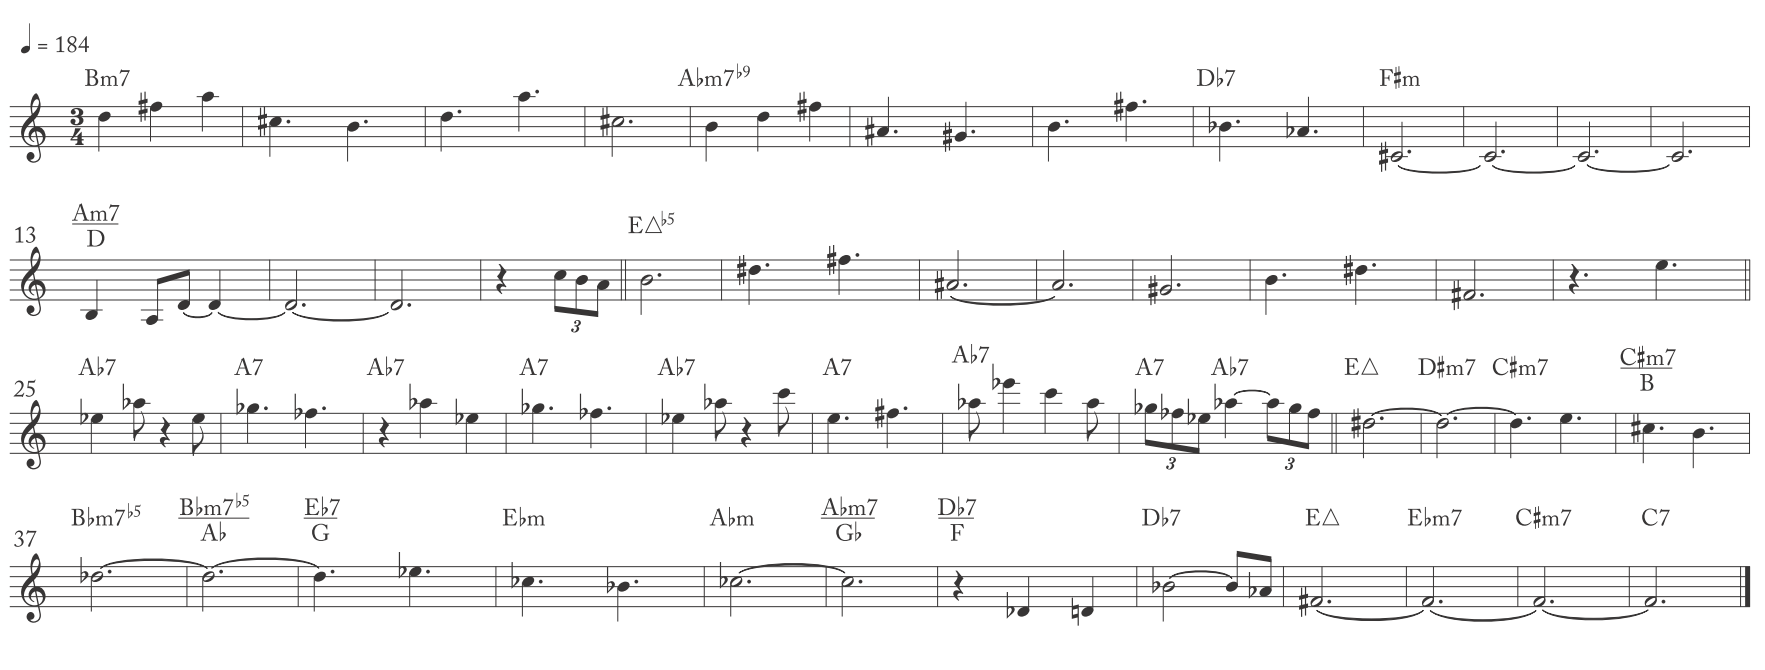
\includegraphics[width=6in]{strunk_windows.png}	
\end{figure}

%Strunk's middleground 1 with extended E prolongation
\begin{figure}
	\centering
	\caption{Strunk's Figure 2, his ``Middleground graph 1" for Corea's ``Windows."  Taken from p.\ 18 of \cite{strunk2016}.}\label{strunk_fig}
	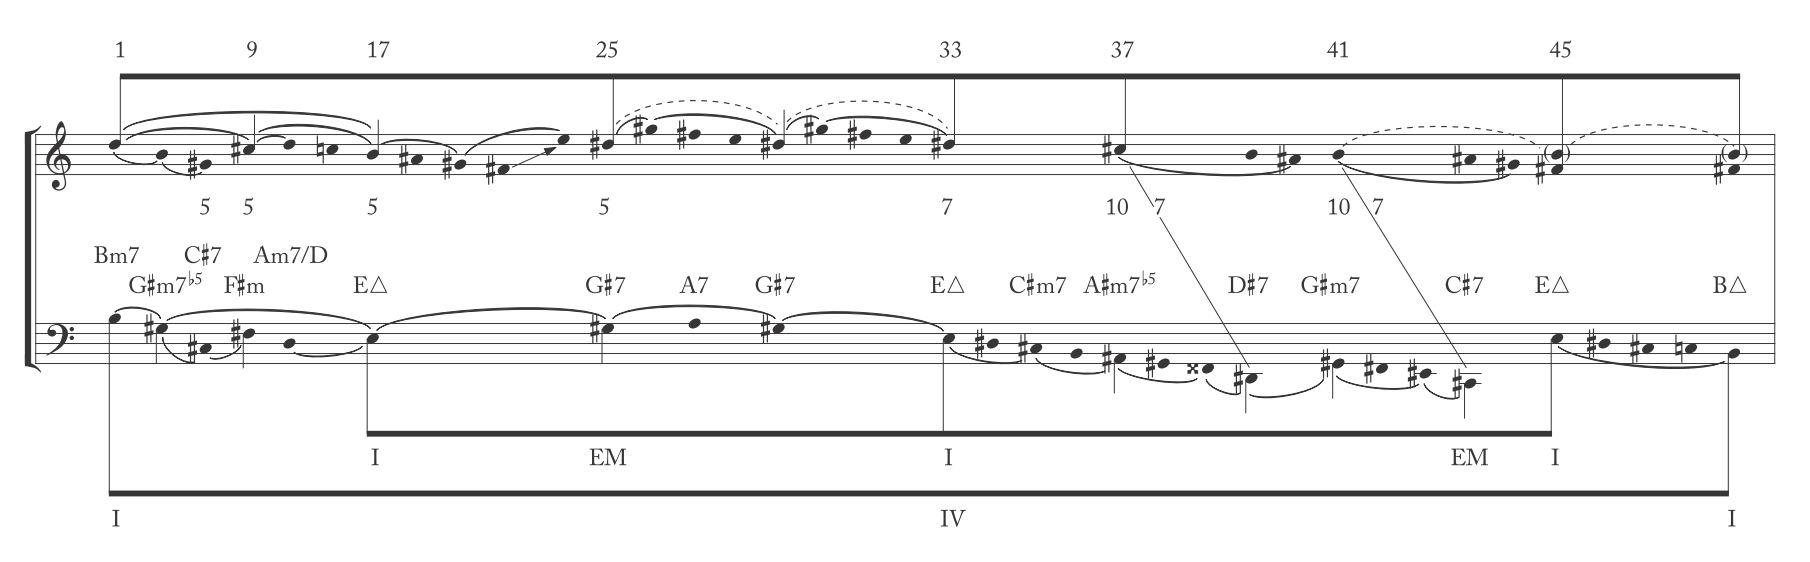
\includegraphics[width=6in]{strunk_windows1.png}
\end{figure}

%Waters
Waters re\"{e}xamines ``Windows" with skepticism regarding the importance of $IV$ as a syntactically functional tonal subdominant, opting instead to describe the piece as a series of ascending fifth-related keys poorly captured by an appeal to the subdominant (or indeed by a monotonal reading in general).  Parsing the tune through the lens of a repeated ascending-fifth ``schema" drawn from Bill Evans's ``34 Skidoo," Waters rehabilitates many of Strunk's embellishing chords as essential stepping stones for a schematic sequence -- $Bm$, $F\sharp m$, $C\sharp m$, $A\flat m$ -- encompassing measures 1-41.  Waters labels the successive ascending-fifth phases of the tune in his Example 2, reproduced here as Figure~\ref{waters_fig}.  Tracing the fifths through the entire tune requires the abandonment, or at least the substantial weakening, of Strunk's $EM$ tonal prolongation.

%Waters's four-stage ascending-fifth schema parsing of Windows
\begin{figure}
	\centering
	\caption{Waters's Example 2, where he parses ``Windows" as a series of ascending-fifth motions.  Taken from p.\ 40 of \cite{waters2016}.}
	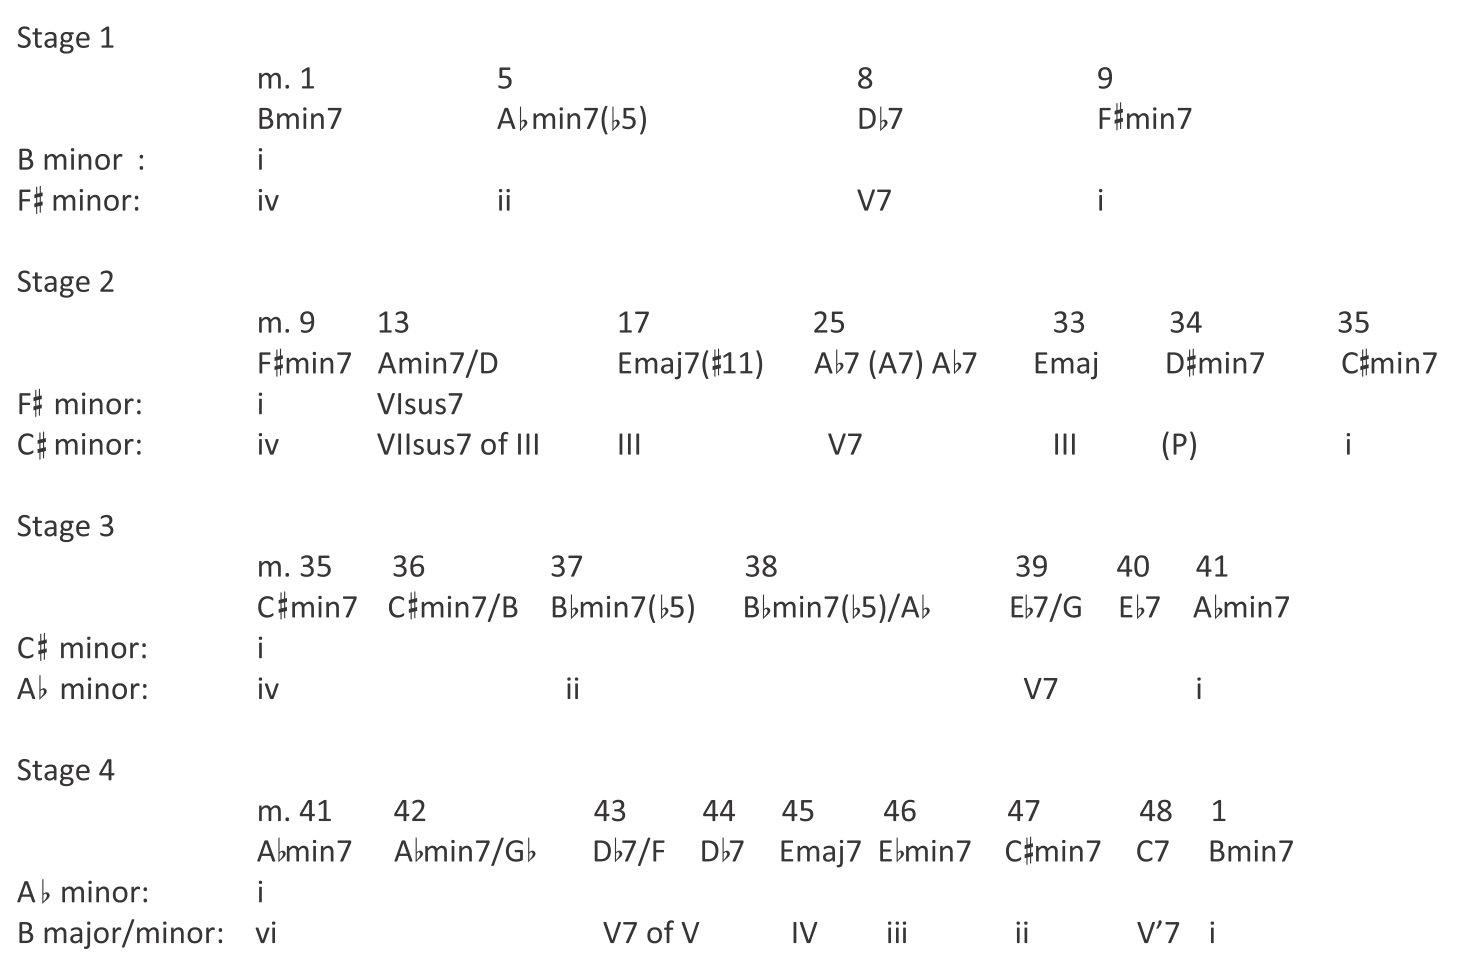
\includegraphics[width=6in]{waters_windows.png}
	\label{waters_fig}
\end{figure}

Waters notes that there are certainly ``compelling reasons" for Strunk's focus on $EM$, including its obvious duration, its hypermetrical placement at the start of two 8-measure phrases, and its appearance at both the beginning and ending of the hypothesized prolongational span.  But here, Waters objects on formal grounds, noting that ``neither duration, hypermetric inflection, nor departure/return is sufficient for prolongation."\footnote{\cite{waters2016}, p.\ 40.}  The usual grounds for prolongation -- presumably, embellishment through common passing or neighbor chords -- are missing, since the prolongation ``is carried out in an unorthodox manner, through $A\flat^7$ (mm.\ 25-32), a harmony in chromatic third relationship with E."\footnote{\cite{waters2016}, p.\ 40.}  Instead, Waters proposes that we hear $EM$ as a relative major substitute for $C\sharp m$, casting his re-labeling as a claim of harmonic relation and temporal delay: ``Thus the mm.\ 33-35 progression EMaj7 - D$\sharp$min7 - C$\sharp$min7 stands for C$\sharp$ minor (with ``stand for" meaning a transformation that meaningfully relates to and delays the more expected C$\sharp$ minor)."\footnote{\cite{waters2016}, p.\ 41.}  If the $EM$ sonorities have a syntactic ``function" in the tune, its primary status is not that of the subdominant of $B$, but rather as a substitute local tonic in $C\sharp m$.

%Waters:Strunk::Wollheim:Loran
I find Waters's analysis rewarding and attentive to the schematic norms of postbop practice, and I will return to his notion of substitutability and ``standing-for" in the next section.  For now, I note that his specific objections to Strunk's analysis echo Wollheim's description and critique of manifest formalism in the work of art critic Erle Loran.\footnote{The Loran discussion comes in \S 12, pp.\ 22-26, of \cite{wollheim1995}.}  In summarizing the argument of Loran's 1943 book on C\'{e}zanne's practice, Wollheim describes a reduction and justification process similar to Strunk's Schenkerian parsing: beginning with C\'{e}zanne's \emph{Still Life with Faience Jug}, reproduced here as Figure~\ref{cezanne}, Loran provides a reductive analytic overlay, isolating and extracting what he sees to be the formal boundaries or outlines of shapes given in the painting.  He then draws ``carry-through" lines designed to track and describe representational, volumetric tension experienced by a viewer.  The two-dimensional outlines give rise to (or represent, or stand as signs for) some phenomenal three-dimensional volumes, and those volumes are relatable to one another in a formal way.  All of this interpretation, Loran states, can be gleaned from the purely configurational (that is, formal, content-free) aspects or indices of the painting.  Wollheim reproduces several of Loran's supporting diagrams, four of which appear in Figure~\ref{loran_diagrams}.

%the cezanne painting
\begin{figure}
	\centering
	\caption{C\'{e}zanne's \emph{Still Life with Faience Jug and Fruit}, from the Oskar Reinhart Collection ``Am R\"{o}merholz," Winterthur.}
	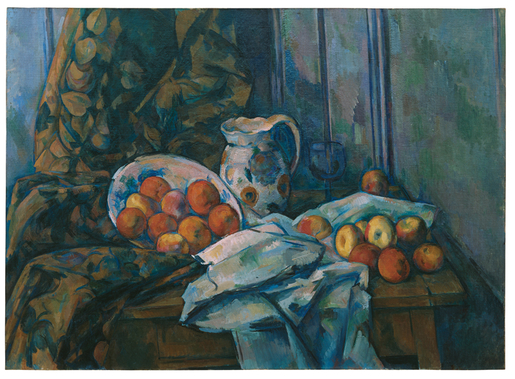
\includegraphics[width=6in]{cezanne.png}
	\label{cezanne}
\end{figure}

%the Loran diagrams
\begin{figure}
	\centering
	\caption{Four of Erle Loran's C\'{e}zanne diagrams, taken from \cite{wollheim1995}, pp.\ 44-45.}
	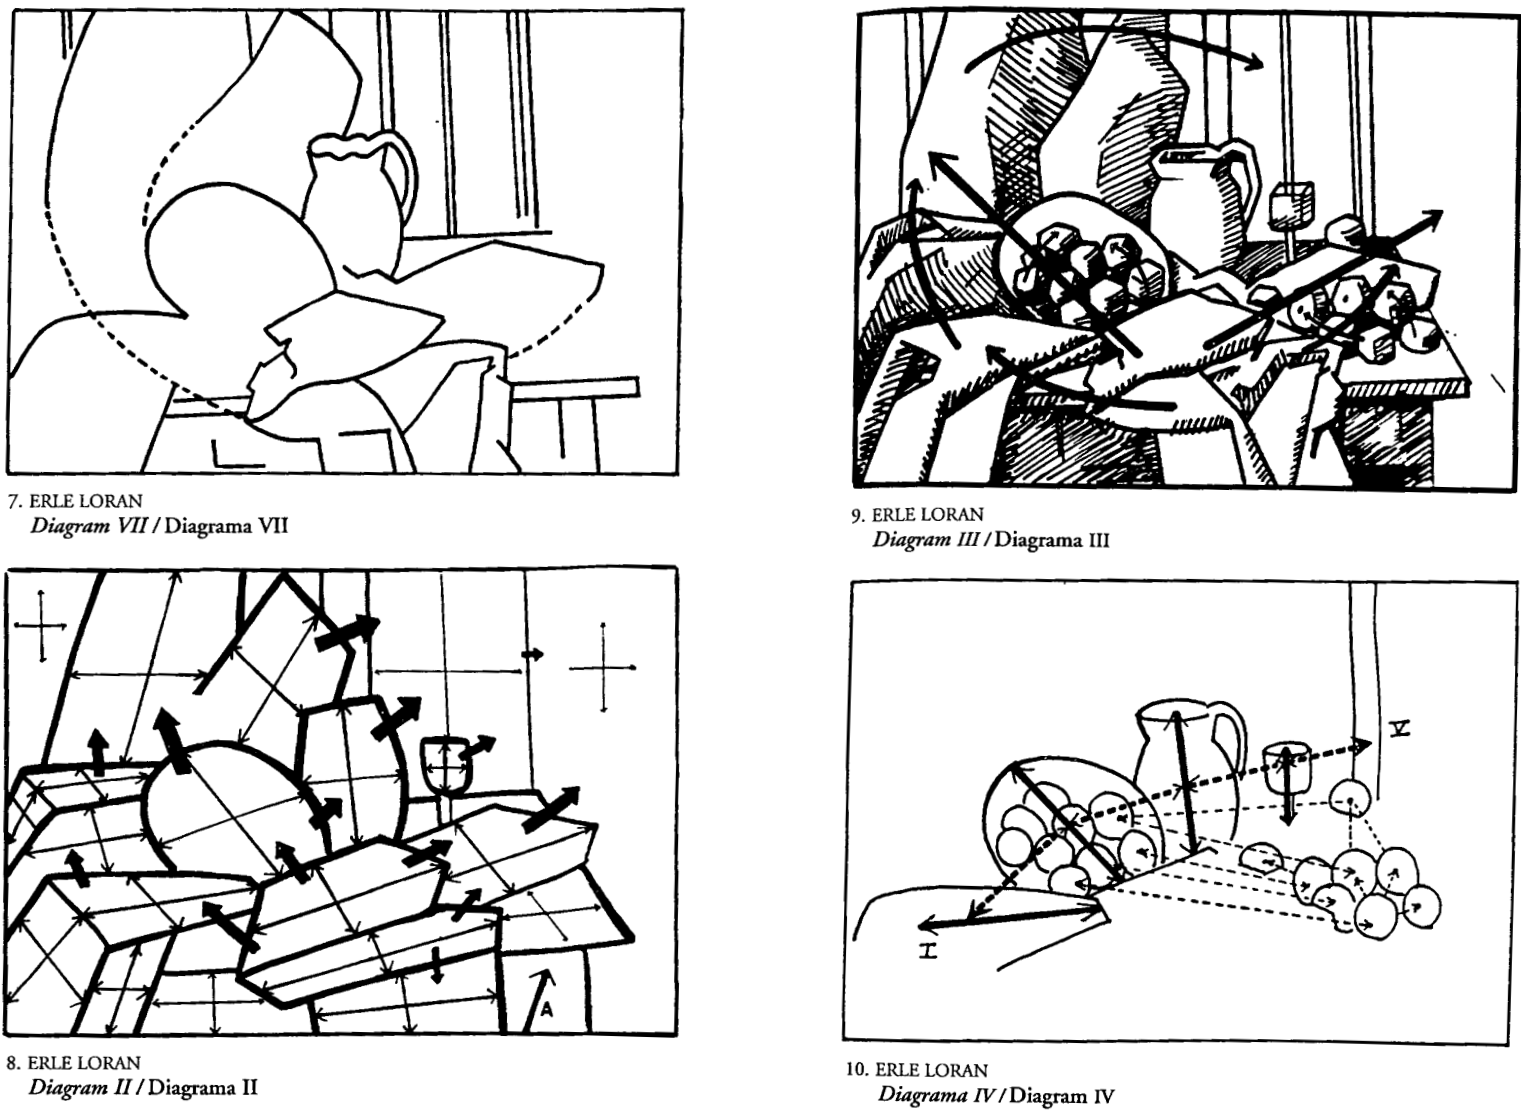
\includegraphics[width=6in]{loran_diagrams.png}
	\label{loran_diagrams}
\end{figure}

Wollheim has two main objections.  First, and more generally, he doubts that the outlines of shapes can be reliably selected from a painting in a consistent and purely formal way, without explicit appeal to the representational content of some viewer.  Judging where a shape begins and ends, Wollheim reminds us, is strongly informed by our internalized norms for the properties of whatever shape(s) and represented object(s) we might recognize in a given visual array.\footnote{Consider Wollheim's discussion of identifying the ``black ring" crowd shape in Breughel's \emph{Christ Carrying the Cross to Calvary} on \cite{wollheim1995}, pp.\ 9-13.}  Second, Wollheim drives a wedge between the two-dimensional outlines and Loran's ``carry-through" lines of three-dimensional tension.  Loran claims that the volumes arise from the formal configurations of the two-dimensional shapes, but Wollheim counters that the moment of turning a two-dimensional array into a represented three-dimensional volume is a psychological one, and that it cannot possibly occur independently of the other (non-formal) aspects of the painting.  As Wollheim puts it in his general rebuttal to manifest formalism, of which he sees Loran's work as a particularly problematic variety,
\begin{quote}
``Observe the earthenware object that lies on the ground on the left-hand side of the picture [Breughel's \emph{Christ Carrying the Cross to Calvary}].  As our eyes alight on it, we recognize it as a domestic vessel.  At this point the beliefs that we have about such utensils confirm us in seeing the dark circle on its body as an aperture opening inwards rather than as a protuberance pushing outwards... [W]e cannot exclude from the formal aspects of the painting any factor that influences what we see in the painting.  And there seems no way in which we can be certain, in advance of particular cases, particular paintings, that some given aspect of a painting will never be such a factor."\footnote{\cite{wollheim1995}, p.\ 22.}
\end{quote}
If Loran's three-dimensional tension is meant to arise from ``the similarity in the objects' size, shape, and colour," Wollheim suggests, ``we know better."\footnote{\cite{wollheim1995}, p.\ 25.}  Noting visual tension between apples in two different locations in C\'{e}zanne's \emph{Still Life with Faience Jug} seems to involve more than familiarity with outlines and colors.  The identification of representational volumes based on shapes in the visual array, the tensions between those volumes, and even the boundaries of two-dimensional shapes themselves depend on more than just the formal indices of the painting \emph{qua} painting: the viewer's multifaceted visual processing both requires and imposes numerous potentially non-formal aspects for and on any particular ``formal" parsing.\footnote{Wollheim's ultimately psychoanalytic commitment to the process of seeing-in and seeing-as is quite complex, and he would likely resist my use of the term ``parsing," here.  His formalist critiques do not necessarily depend on the adoption of his strikingly Freudian psychoanalytic representational stance, a thorough consideration of which may be found in \cite{davis2010queer}, Chapter 10.}

%TODO: this would be one spot for a Kockelman translation of Wollheim.  It could also come after its application to Strunk/Waters.

With the caveat that translation of Wollheim's argument into musical form requires both nuance and skepticism, Waters's response to Strunk can be paraphrased in Wollheim's terms and leveraged toward a paradigmatic critique.  Like Wollheim's manifest formalists, Strunk purports to examine the musical surface and extract (trace) the important harmonies, those that control, prolong, or function as boundaries for tonal spans (shapes).  Reducing away voicings and embellishing chords, Strunk shows an E Major ``shape" as an important formal property of Corea's tune.  With attention to schema drawn from jazz practice, Waters sees a different tonal shape in the passage, and he challenges Strunk's identification of an EM prolongation in a way directly analogous to Wollheim's critique of Loran: Strunk's identification of the formal prolongation seems based on his selection of important musical indices which are, nevertheless, not ``sufficient for prolongation."  To see the shape of the tonal prolongation Strunk identifies, we cannot simply extract surface-level chords to provide a formal justification; like with C\'{e}zanne's apples or Breughel's jug, our identification of the prolongation is dependent on features other than surface harmonic analysis.  If those other features are the ground on which the prolongation rests, no diagram of the type Strunk offers can furnish sufficient proof of its existence.  To put it in Wollheim's words:
\begin{quote}
``Though, through the use of diagrams, [Loran] can analyze, on the one hand, how the artist organizes the picture-plane and, on the other hand, how he organizes the represented space, what, in the nature of things, Loran cannot present diagrammatically is the meeting-point of the two, which is, for him, precisely where C\'{e}zanne's pictorial achievement, indeed pictorial achievement in general, lies... In order to grasp just how C\'{e}zanne fused the organization of volumes and the organization of the picture-plane, we have to go back to the painting itself and experience the fusion: nothing else will do.  There is no formulaic representation of the crucial stage."\footnote{\cite{wollheim1995}, pp.\ 24-25.}
\end{quote}
Since Strunk's prolongational reductions do not represent the moment where the surface harmonies somehow generate or map onto the tonal prolongation he suggests, the prolongation itself can be challenged.  Waters can provide an explanation appealing to a totally different paradigm: the passage might not need to form the shape of a tonal span in the subdominant, but rather could be seen as a series of ascending fifths.

%paradigm comparision, Schenkerian drive-by
The paradigms in play, here, make use of different terms and proof structures-- they start from different ``shapes," and they ``trace" those shapes in different ways.  Strunk's Schenkerian reductions begin with harmonic norms drawn from tonal, western-classical music, and they demonstrate a kind of tonal coherence by selecting surface features from ``Windows" to generate a hierarchy of important tonal features and regions.  Waters's schematic analyses begin with harmonic schema drawn from postbop jazz, and they demonstrate a replicatory chain of influence by interpreting surface voicings in a way designed to show their compatibility with repeated application of the same schema.

The algorithmic statements of the preceding chapters cannot reproduce manifest formalist claims of the variety employed by Strunk and other Schenkerian-prolongational theorists.\footnote{It comes as no surprise that the earliest intersections between programming and Schenkerian analysis center around encoding analyses as generative linguistic trees -- parsing trees may be stored in memory, and explicit unfoldings and motions up or down the tree may be cued by the human analyst in communication with the (entirely pre-specified) terminal tree (see \cite{smoliar1979}).  Smoliar is aware that this activity requires more than surface-structural claims, noting that ``while the information base of chord grammar is simply the vocabulary in which the labels are expressed, it is somewhat harder to characterize explicitly the information required to express chord significance" (p.\ 110).  For his and later computational Schenker projects, linguistic hierarchical descriptions of this ``significance" carry a definitional importance inaccessible to my algorithmic agents, and they require span-identification and elaboration rules passed explicitly from human analyst to algorithmic interpreter.  Among many more contemporary grammatical implementations, see \cite{mavromatis2004} and \cite{marsden2010}.}
And while these un-reproduced claims count against a temporal-syntactic paradigm, in one sense, they may be unreproducible for good reason: it may not be possible for data drawn exclusively from the surface-level harmonic content of jazz performances and interpreted by algorithmic agents to demonstrate Schenkerian claims of tonal harmonic prolongation, since the sense-making of such span-identification might \emph{require} human preconceptions regarding spans.\footnote{The broader question of how the rules for identifying Schenkerian prolongational spans might (or might not) be learned from musical surfaces partly resurrects the highly contentious 1978-1979 exchange between Keiler and Jackendoff and Lerdahl.  My re-framing of Wollheim's objections to manifest formalism bears direct resemblance to Keiler's questions regarding the ``discovery procedures" necessary for constructing a Schenkerian musical grammar. As Keiler writes, ``The circularity inherent in the notion of discovery procedures lies in the fact that the question of their internal logic or consistency depends necessarily on the kinds of analytic judgments intended in the first place" (Keiler 1978, p.\ 182).  See \cite{keiler1978}; as well as \cite{jackendoff1979}; \cite{keiler1979}; compare to my \S 1.4 above.}  Those preconceptions do not seem machine learnable, to me, though I consider the problem open.  In any case, the data representation and pipeline of Chapters 2-4 align algorithmic agents toward the production of other kinds of interpretant, and the ontological conditions these agents employ for segmentation and generalization are incompatible with robustly Schenkerian prolongational concerns.  Waters's claims, to the extent that some of them are predicated on parsing jazz progressions in terms of repeated harmonic schema, may lend themselves to a corpus-syntactic paradigm more easily; as such, they (and my own claims) may better resemble what Wollheim calls \emph{latent} formalism.

\subsection{Functional Analysis as Latent Formalism}
%Finish up Waters as grammatical/quasi-statistical latent formalist
%Terefenko's functions as syntactic latent formalism
%Wollheim's segmentation objection as motivating my project, which doesn't completely solve the problem

%Start with Terefenko-style functional analysis claims
If Strunk's prolongational analysis of Chick Corea's ``Windows" can be described as a kind of manifest formalism, as my Wollheimian extension of Waters's response implies above, it stands as one type of claim regarding jazz harmony unreproducible under the corpus-syntactic paradigm of Chapters 2-4.  Manifest formalism does not exhaust the space of unreachable claims, however; two other paradigmatic modes of discourse on jazz harmony seem not to find a statistical home -- pedagogical approaches and functional analyses of individual tunes or performances.  As an exemplar for both of these varieties of inquiry, I turn below to the jazz manual of Dariusz Terefenko.\footnote{\cite{terefenko2014}.}  I aim to unpack Terefenko's textbook partly as a latent formalist project, in Wollheim's terms, and I will ultimately suggest that my own work inclines in this direction, as well.

Terefenko does not aim his book at music theorists, at least not directly; rather, the text is meant for dedicated, adventurous musicians, ``undergraduate and graduate jazz students, and for an ever-increasing population of classical students interested in jazz theory and improvisation."\footnote{\cite{terefenko2014}, p.\ xv.}  As such, the book takes a fair amount of western-classical theoretical assumptions as a ground, providing quick primers on scales, meters, triads, and roman numeral analysis designed as reminders rather than explicit theoretical claims.  Since Terefenko presents theory in the service of practice, I will not subject his claims to quite the same critical attention as those in theoretical works like Strunk's or Waters's.  But attending to the model implicit in most of the book will, nevertheless, clarify one of the major presentational paradigms in jazz pedagogical literature.

While Terefenko's descriptions for phrase models and song forms presented in Part Three invoke Schenkerian techniques, the earlier portions of the book treat prolongation with a light touch, instead presenting a wide array of chords through the lens of functional categories.  Terefenko describes harmonic function quasi-grammatically from the outset:  after introducing tonic, predominant, and dominant as the necessary components (or ``contextual features") of functional tonality, he describes their properties and proper concatenation into phrases in terms of tension and release patterns.  The restful stability of the tonic, the moving-away of the predominant, and the tense instability of the dominant are all ``different behavioral patterns," which ``remain constant across the entirety of the tonal system in which jazz forms a distinctive musical language with its own harmonic grammar and melodic syntax."\footnote{\cite{terefenko2014}, p. 26.}  But even as Terefenko firmly grounds jazz harmonic function within a western-classical tonal paradigm, he makes space for its own idiomatic dialect: ``As will be demonstrated time and time again, functional tonality in jazz has different properties than that of common-practice classical music.  These properties are represented by a unique set of rules dictating the unfolding of harmonic function, voice-leading conventions, and the overall behavior of chord tones and chordal extensions."\footnote{\cite{terefenko2014}, p.\ 26.}  Much of the rest of the book is dedicated to stipulating these rules and showing examples of jazz harmony's idiomatic grammaticality.

%Use Wollheim to describe them as latent formalism
As Terefenko assigns a plethora of jazz chords to the three basic functional categories, he builds the lexicon of a complex grammatical system with a comparatively simple syntax.  The tonic, predominant, and dominant, which exist as idealized parts of musical speech, occur in a small number of grammatical orderings; most of the interest in jazz harmony, for Terefenko, consists of complicated mappings from increasingly dissonant chords to their interpretive functional categories.  Parsing musical surfaces toward this end produces what Wollheim would call a latent formalist system, where the harmonic drama arises from the underlying syntax of progressions.  Wollheim offers an extremely clear description of linguistically-inspired latent formalist models, claiming that rules of syntactic organization must meet five requirements:
\begin{quote}
(one) they presuppose some way in which larger units can be segmented into smaller units, and ultimately into basic units;

(two) they then operate on the basic units, which they first classify under certain general categories.  In the case of language, examples of such categories are noun, verb, adverb;

(three) they order these elements, classified by category, into strings of elements that are well-formed, or grammatical, while all other strings are ill-formed, or ungrammatical;

(four) the rules function recursively, in that they can be endlessly reapplied to their own output so as to yield an unbounded set of further well-formed strings; and

(five) in those cases where the strings refer, or have a semantic dimension -- that is, in all cases except purely formal languages -- the meaning that each string has is determined by its syntactical form plus the vocabulary, or lexicon, of the language.\footnote{\cite{wollheim1995}, pp.\ 26-27.}
\end{quote}
Terefenko's functional harmonic syntax engages with each of these requirements.  He explicitly states that passages of varying length can carry functions or be divided into elements which do so; he classifies those harmonic elements into functional categories; he deploys the elements (usually chords) in well-formed progressions, repeatedly and with variation.  If Terefenko's musical strings (usually harmonic progressions) do indeed refer, along the lines of Wollheim's fifth requirement, their semantic dimension might encompass a particular tune or style of playing, both of which are presumably recognizable from the combination of functional syntax and a particular lexicon, be it voicings or head changes.  But setting aside musical semantics, a proper analysis will reveal the hidden (latent) syntax of a given passage, and a proper composition will follow the grammatical production rules for ordering categories to produce an intelligible tune or improvisation.

For formalist projects of this general type, Wollheim offers another critique.  Taking to task Yve-Alain Bois's semiological description of Picasso's Cubism, Wollheim shows that a supposedly-syntactic analysis of Picasso's \emph{Head of a Girl} or Grebo mask must fail to satisfy the requirements given above.  Three of Wollheim's objections find possible counter-arguments in Terefenko's syntax.  Wollheim claims that Bois ``proposes no categories analogous to those of grammar," while Terefenko does; Bois offers no rules for how to concatenate categories, while functional harmony does this, in a general sense; and Bois offers no sense of what un-grammatical works of art might be: ``He gives us no reason to think that pictorial objects can be divided into the well-formed, which are legitimate, and the ill-formed, which are illegitimate, where this division is effected on the basis of whether or not rules of a very specific kind have been properly applied in their production."\footnote{\cite{wollheim1995}, p.\ 30.}  If one of Terefenko's students is expected to improvise with other musicians and write tunes in a mutually-understandable idiom, there may well be social and grammatical norms separating well- and ill-formed utterances.  Terefenko's functional harmony avoids many of Wollheim's latent formalist objections.

Terefenko's functional syntax may not, however, satisfy one of Wollheim's objections:  Wollheim complains that Bois offers ``no systematic way in which the total surface of the pictorial object could be segmented-- segmented, that is, without remainder-- into parts, which could then function as syntactical constituents."\footnote{\cite{wollheim1995}, p.\ 29.}  When confronted with a complex visual array, a Boisian latent formalist must somehow decide both how to chop up the painting into syntactic elements and how to recognize each element as part of the appropriate grammatical category.  This segmentation difficulty has an auspicious musical history in atonal music theory,\footnote{See its explication at the end of Part 1 of \cite{forte1973}.} but it applies to Terefenko's contextual parsings, too.

As one parsing example among many, consider the simple tonal progression on his p.\ 33, reproduced here as Figure~\ref{Terefenko_ex}.  For Terefenko, several of the chords can be given \emph{a priori} functional assignments based on their pitch structure -- in the limiting case, Terefenko has given the student no category other than tonic for the minor $i$ chord, but $V$ and $ii^\circ$ also seem unambiguous, here.  The $VI$ chords of measures two and four, however, merit special consideration:
\begin{quote}
The third chord of the progression, the submediant also has two functional assignments: tonic and predominant.  Based on the surrounding context though, especially the forthcoming $iv$, the $VI$ can be interpreted as belonging to the predominant family of chords.  The predominant $ii^{\circ}$ in m.\ 3 forms a cadential gesture with the dominant that then resolves deceptively to the $VI$.  Given the two functional assignments of $VI$, it functions as a tonic in the context of this progression.
\end{quote}

\begin{figure}
	\centering
	\caption{Terefenko's Figure 3.10, a tonal progression in minor.  Each chord receives a roman numeral based on its pitch structure, and Terefenko employs a multi-level parsing to assign functional categories to each roman numeral, starting from the clearest cases and extrapolating to ambiguous ones.}
	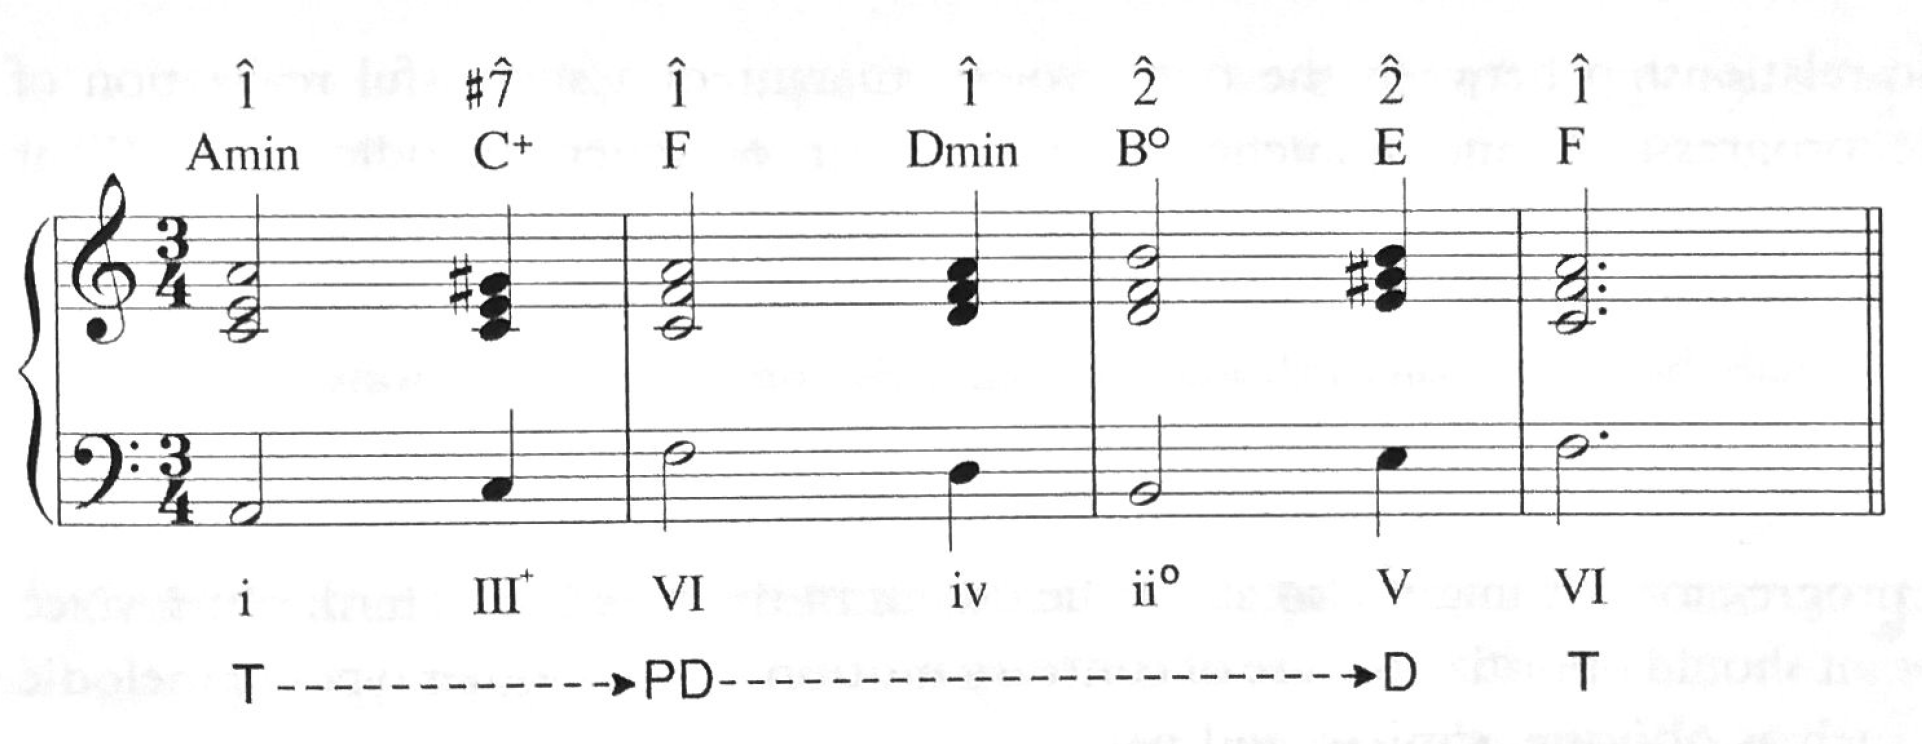
\includegraphics[width=5in]{Terefenko_ex.png}
	\label{Terefenko_ex}
\end{figure}

The segmentation procedure Terefenko employs is sensitive and emblematic of latent-formalist jazz analyses: begin by assigning a rooted, tertian-stack roman numeral label to each sonority, and consult a table of functional assignments to determine the category to which each roman numeral belongs.  When the category assignment is ambiguous, fall back on the local context of the phrase, tracing a quick hermeneutic loop designed to produce whichever functional label best fits the analyst's expectation for normative behavior in the local context.  In Terefenko's words, ``The surrounding harmonic context in which chords occur determines the analytical interpretation of these chords."\footnote{\cite{terefenko2014}, p.\ 33.}  If that is true, then the assignment of particular chords to functional categories does not depend (or, more charitably, does not \emph{only} depend) on their pitch structures, despite the fact that the rest of Terefenko's material on harmonic function makes repeated reference to pitch-based tables of harmonic functional categories.  The implied segmentation procedure is not \emph{a priori} consistent, and it requires foreknowledge of which contextual forces will override the pitch-based category assignments found in elementary descriptions of tonic, predominant, and dominant.

This hermeneutic circle at the heart of functional parsing renders harmonic analysis flexible and fertile, but it also renders any truly latent formalist system incomplete or circular.  If there is no explicit account given for how functional assignment is to be accomplished without recourse to the analyst's expectations, the formalist parsing runs the risk of confirming any preconceptions the analyst has.  As I claimed in Chapter 1's discussion of Lerdahl \& Jackendoff -- also latent formalists, much more explicitly -- the ``rules" of syntax cannot be proven on the basis of analyses of this kind, as contextual parsing will allow the analyst to shoe-horn a wide variety of musical surfaces into the analyst's pre-existing theory of harmonic syntax.  Terefenko is able to avoid an explicit framing of functional category assignment precisely because the paradigm under which he operates assumes one implicitly: the pedagogical analysis of particular passages implies a set of top-down ``rules" to be taught to the student, and the application of those rules results in claims about the music at hand.  Whether those claims are meant to encompass how the teacher hears the music, how the student ought to hear the music, or something about the structure of the music independent of a hearer cannot readily be determined within the paradigm's framework.%last part of this paragraph is weak

%Wollheim's objection motivates my project
Latent functional analysis for pedagogical purposes may yet be re-writable under a temporal syntactic paradigm, but Wollheim's segmentation objection must first be dispatched: the data-driven temporal segmentation and clustering performed in chapters 2-4 is an attempt to do so.  Where Bois cannot separate elements within the Grebo mask, chapter 2 suggests that voicings or scale-degree sets might be extracted from YJaMP based on their temporal properties -- that we can consistently partition the notes of a performance based on the perplexities of time-window note distributions and statistical patterns of inter-onset timing.  Where Bois cannot give an account of what general categories of syntactic behavior might exist for elements of the mask, and where Terefenko assumes pre-existing western-classical functions, chapter 3 suggests that statistics regarding temporal behavior on different time scales can serve as a ground for a kind of syntactic functionality.  And where Bois cannot provide meaningful rules assigning elements of the mask to syntactic categories or ordering them, Terefenko relies on hermeneutic application of western-classical functional patterns.  Chapter 4 suggests that clustering chords based on similarities in their PCA-reduced temporal properties provides a starting point for functional assignment independent of many analytical pre-conceptions, but the process described there accomplishes a task quite different from  Terefenko's harmonic parsings.  Unlike Wollheim's art-theoretical critique, a corpus of jazz piano harmony permits linguistically-inspired latent formalist description accountable to musical data.  Whether the resulting description still permits productive hermeneutic engagement with individual tunes for students and analysts is an open question.

\section{Paradigmatic framings}
%kockelman here, and use it to reframe the historical and latent formalism above
Wollheim's objections to manifest and latent formalism survive (or benefit from) translation into semiotic ontological terms. Pulling his criticisms apart across Kockelman's semiotic diagrams allows the specification of blocked or successful channels of communication between agents, stable or unstable objective ontologies, and interpretants produced through parasitic means.  With these framings in hand, I will be in a position to suggest what kind of semiotic processes the corpus analytical pipeline of chapters 2-4 affords; the resulting latent formalist framing co-generates objects and analysts well-aligned for only certain modalities of syntactic interpretation.

\begin{figure}
	\centering
	\caption{Formalist parsings implied by Loran and Strunk (top) as subject to critiques by Wollheim and Waters (bottom).  Both criticisms may be thought to split and re-frame the parsings into chains of semiotic processes.}
	\label{critiques}
	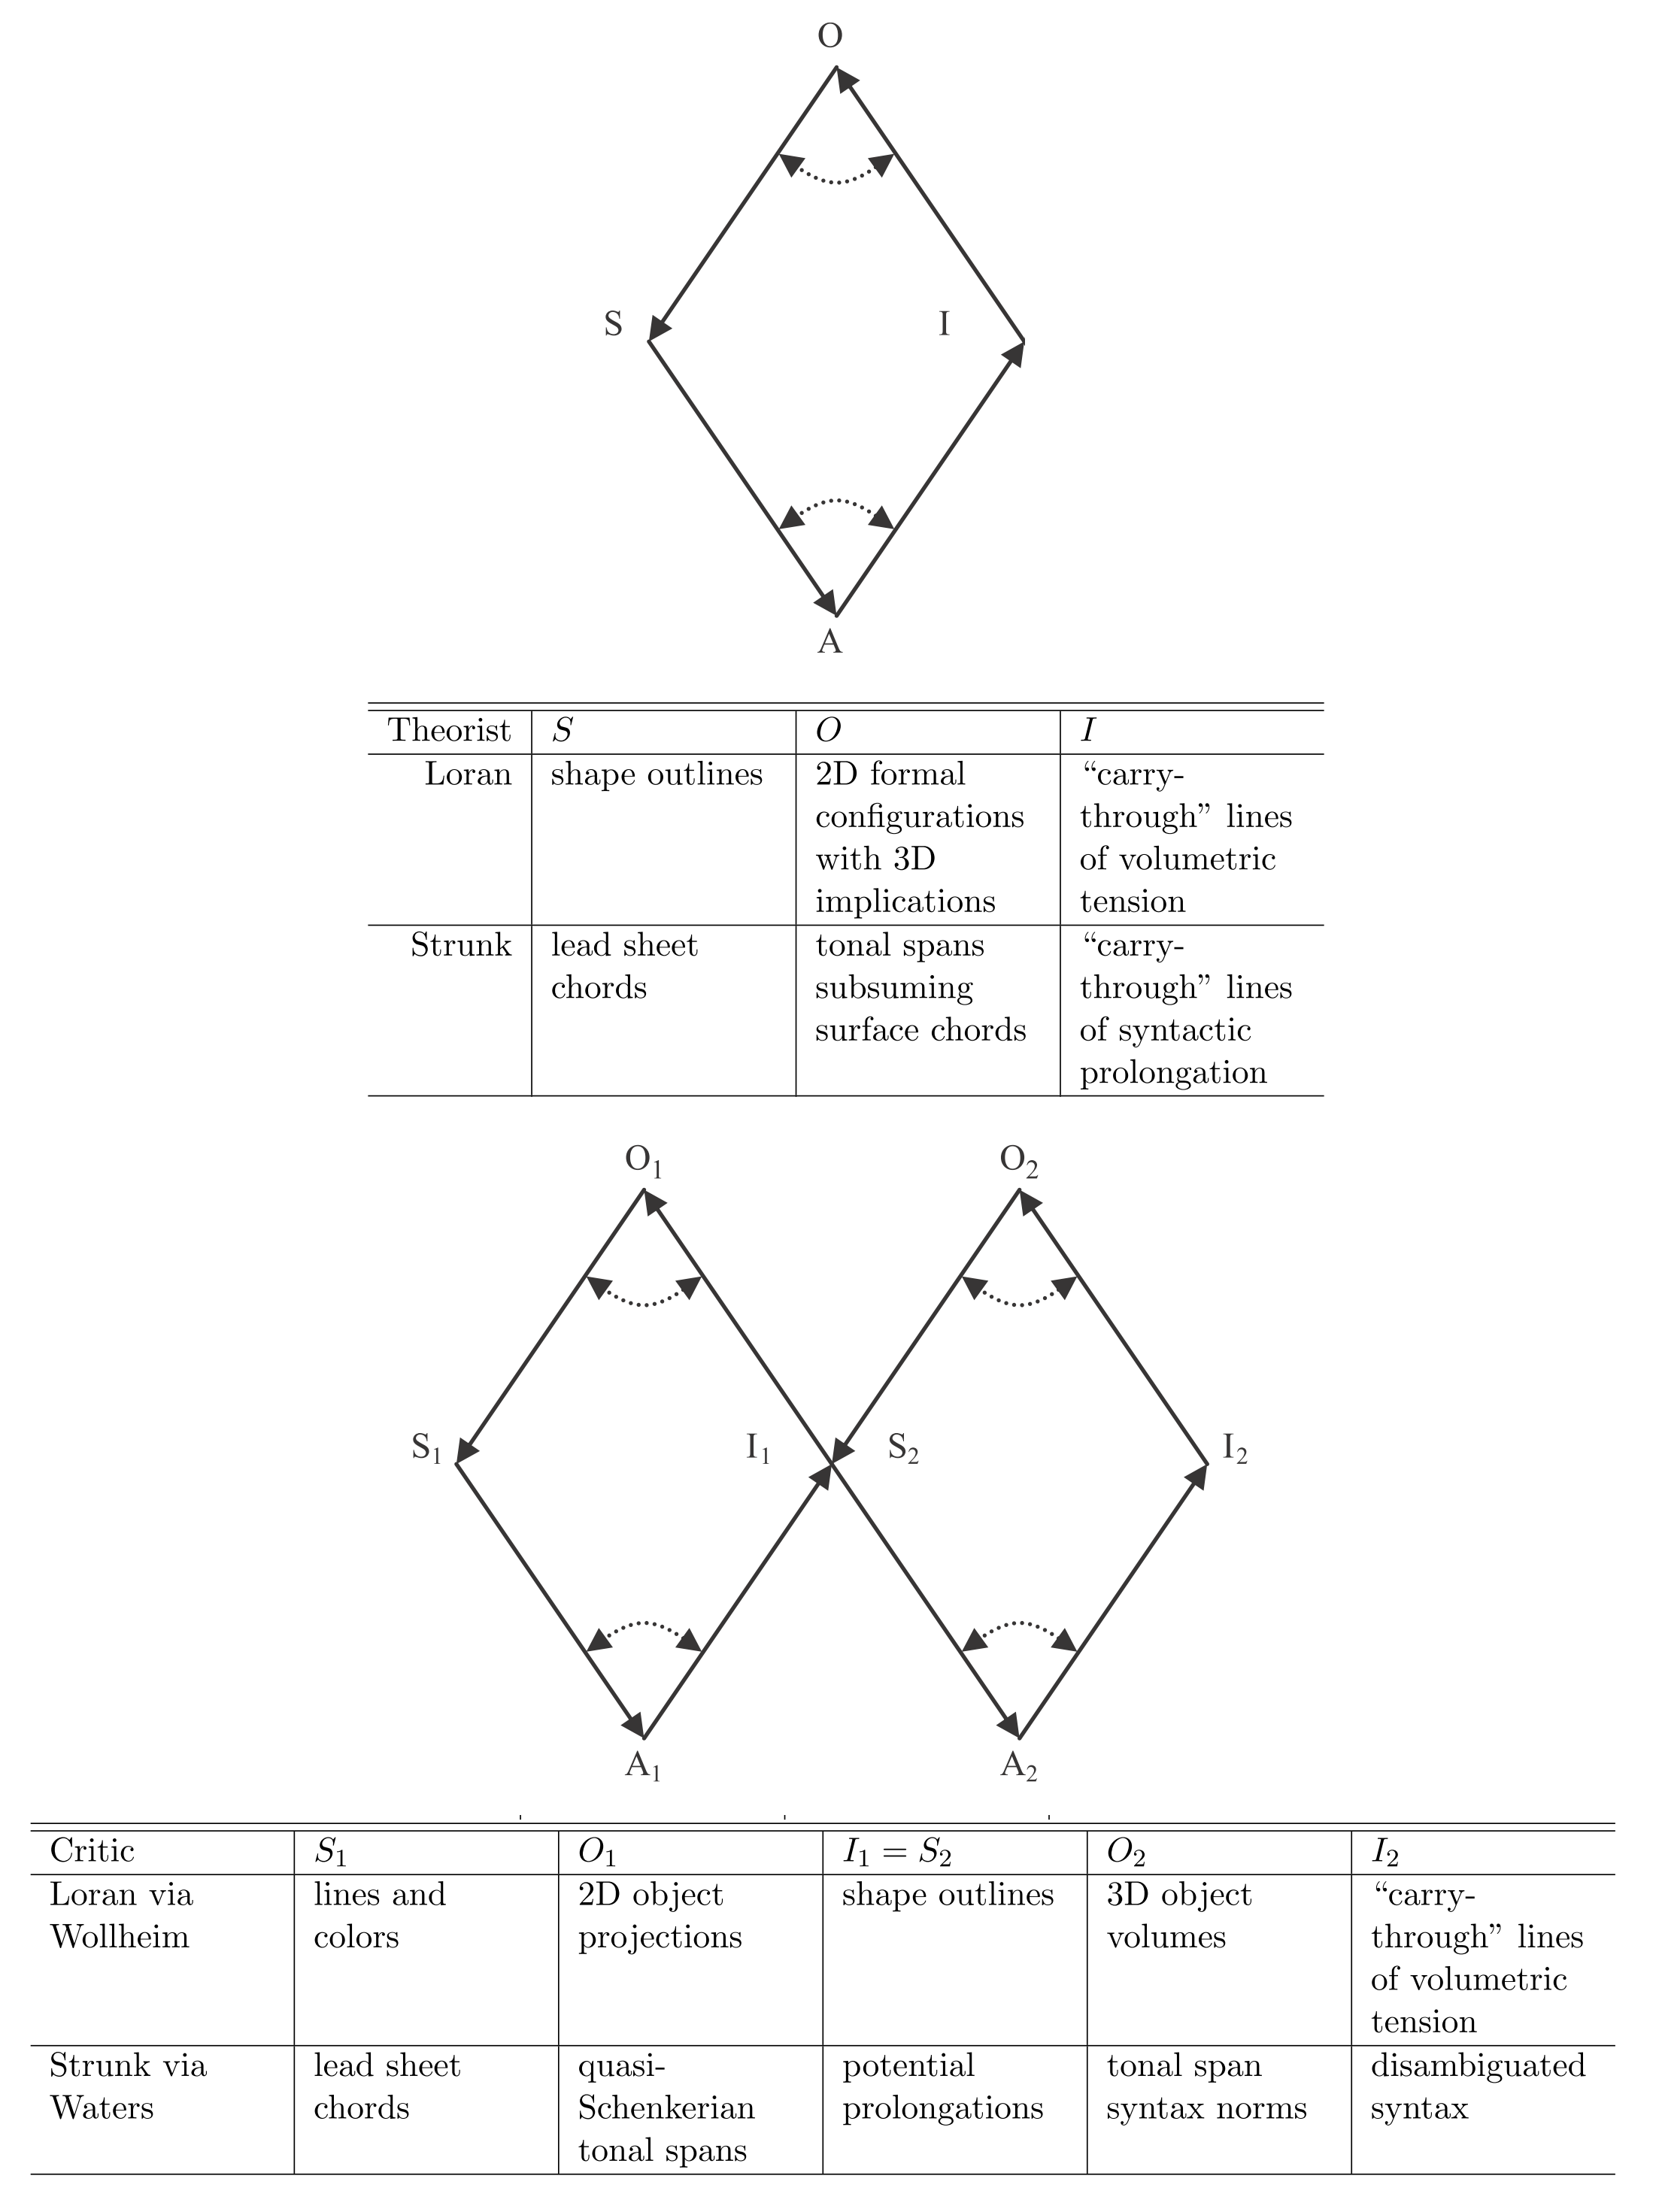
\includegraphics[width=6in]{critiques.png}
\end{figure}

The top half of Figure~\ref{critiques} provides one possible framing for the formalist analyses of Loran and Strunk.  In broadest strokes, each mode of analysis purports to begin with surface features, indices $S$ directly sensible by the analyst $A$.  As Loran would have it, these are two-dimensional shape outlines observable on a painting; for Strunk's analysis of ``Windows," these indices are the chords of the published lead sheet.  Both analysts interpret these indices as signs standing for some kind of object ($O$), and they produce analytical interpretants ($I$) meant to make sense given its properties.  Both produce graphical interpretants (which often serve as indices for other semiotic processes): Loran's ``carry-through" lines of projected volumetric tension and Strunk's tonal syntactic prolongations.  Coincidentally, both use roman numerals as part of their interpretants.  More consequentially, both give meaning to their interpretants with both the observed indices and the properties of spans, objects, or configurations not identical with the observed surfaces.

For Loran to turn shape outlines into carry-through lines, his actions necessitate the existence of objects with two-dimensional formal configurations and three-dimensional volumetric implications -- only in light of both of these kinds of property can the relation of $I$ to $S$ make sense for $A$ (Loran).  For Strunk, prolongational sketches only make sense given the existence of mostly-Schenkerian tonal spans subsuming surface chords.  These spans have some surface chords as observable indices, but the carry-through lines do not merely identify the repeated appearance of those indices -- rather, they make sense given some aural, psychological, or acoustic properties of the tonal span objects.

Wollheim's challenge to Loran and Waters's critique of Strunk appear in the bottom half of Figure~\ref{critiques}, where I interpret each critique as a further specification of (two of) the multiple semiotic framings involved in the production of Loran and Strunk's interpretants.  Wollheim doubts that the formal configuration objects produced by Loran's framing can arise from or connect to the indices of the paintings in a reliable (and representation-free, as Loran would have it) way.  He pulls apart the identification of shapes, noting that Loran really sees lines, dots, colors, shades, and so forth ($S_1$), not shape outlines. He must first interpret those indices as shape outlines -- and an analyst doing so will almost certainly make explicit or implicit reference to his or her experience with the two-dimensional projections of objects in the world.  Tracing a pot-shape involves recognizing a pot; it is not na\"{i}ve.\footnote{I note in passing here that an algorithm \emph{could} trace a pot without any possibility of knowing what it ``is."  In that case, the interpretant produced by the tracing algorithm (that is, the ``shape") would make sense given the properties of a different class of object with a different ontology -- not shape-schema drawn from objects in the world, but some specifications encoded in the algorithm (like recognition of lines and colors, continuity and discontinuity, and so forth).  An algorithm identifying a shape might produce a similar-looking interpretant to a human identifying the ``same" shape (i.e., ``CIRCLE"), but the two are imbricated in quite different semiotic structures.  The price of the consistency offered by the algorithm is that it may not serve ends a human would pursue.  This leads directly to considerations of semiotic parasitism, as will return below at more length.} The analyst then interprets these shape outlines ($I_1 = S_2$) in order to produce lines of volumetric tension which make sense given the properties of three-dimensional objects in general ($O_2$).

In a framing of this kind, Kockelman often notes that the relation between $A_1$ and $A_2$, the agent performing each of the analytical tasks required of Loran, is mediated by the relation between the objects they are selecting and signing, $O_1$ and $O_2$.\footnote{For example, see Kockelman's semiotic discussion of Aristotelian and Marxist ``social relations" as ``a relation between people mediated by a relation between things, where both these modes of relationality are themselves grounded in significance and selection."  \cite{kockelman2013}, p.\ 38.}  For the production of shape outlines to be purely formal, or based only on the configuratedness of the painting, $A_1$ should not consider three-dimensional properties of particular things in the world $O_2$ -- those are emphatically not indices observable on the painting's surface.  But while the signed objects $O_1$ have two-dimensional surface properties recognizable as shape outlines, Wollheim notes, interpretation of their shapes is impacted by exactly that knowledge (that is, the properties assumed by $O_2$).  The communicative relation between the analytical agents of the two framings (be they unconscious psychological processes or Loran in two conscious modes of analysis) is transacted through and mediated by the relations between these objects.  If $A_2$ cannot accomplish its tasks based purely on the painting's formal indices, neither can $A_1$; and if the properties of $O_2$ can determine the properties of $O_1$, then so can the representational analyst $A_2$ exert authority over the ``formal" parsings of $A_1$.

As explicated by Waters, Strunk's implied manifest formalism involves a similar framing.  The prolongational identification in ``Windows" is accomplished by selecting musical surface indices $S_1$ and using them to identify tonal spans $I_1$.  As Waters points out, this identification is, on purely formal terms, underdefined; some surface indices support it, like metric and hypermetric placement, but no obviously Schenkerian harmonic elaborations appear. Since no formal span-identification underpins Strunk's prolongations, several possible spans might be identified ($I_1$).  These spans then serve as indices for another process, by which Strunk must decide that the syntactic context of one particular prolongation makes it more probable -- more well-formed, in linguistic terms -- than other possibilities.  Agent $A_2$ employs a kind of syntax norm to turn potential prolongations into the final syntactic analysis Strunk offers, while agent $A_1$ is meant to rely on purely surface features ($O_1$).  Again, the $O_2 \rightarrow O_1$ relation mediates the $A_2 \rightarrow A_1$ relation: the identification of the prolongational spans cannot be accomplished based only on surface features, but rather is informed by pre-existing expectations regarding harmonic syntax.  This is not disqualifying, especially since Strunk's expectations largely align with those of other experienced jazz analysts.  Waters, however, suggests an alternative: well-formed, syntactic spans in post-bop jazz might have different schematic norms from Schenkerian prolongations (say, $O_{2^{\prime}}$), which might have a different influence on the properties of tonal spans ($O_{1^{\prime}}$).  The identification of tonal prolongations does not provide a proof of Strunk's functional parsing, since that identification already involved a particular semiotic communication between related agents -- and other types of syntax might align with or determine other types of ``prolongation."

As he lays out the case for a repeated-schema parsing of the syntax in ``Windows," Waters frames a pair of semiotic processes relying more explicitly on latently syntactic categories of temporal progression behavior.  From lead sheet chords, Waters produces potential schema segmentations $I_{1^{\prime}}$ which make sense given the properties of schema ($O_{1^{\prime}}$), which have particular surface chord indices and repeat in time.  Ambiguous schema segmentations are then adjudicated ($A_{2^{\prime}}$) by analytical appeals to categories of syntax-preserving chord substitutions ($O_{2^{\prime}}$).  If ``the mm.\ 33-35 progression EMaj7 - D$\sharp$min7 - C$\sharp$min7 stands for C$\sharp$ minor," as Waters writes, it must bear some similarity to it. Waters describes his semiotic standing-for as ``meaning a transformation that meaningfully relates to and delays the more expected C$\sharp$ minor."\footnote{\cite{waters2016}, p.\ 41.}  The temporal context in which the progression appears both permits and modifies a statistically-normative syntactic progression.  These considerations still impact the selection of schema accomplished by $A_{1^{\prime}}$ in a way not \emph{a priori} better or worse than Strunk's framing.  A different semiotic pipeline connects the syntactic disambiguation to the musical surface, and it employs objects with different properties to segment the surface and assess its well-formedness.

%transition to Terefenko and latent formalism
These analytical programs rely on the production and identification of spans with particular surface and non-surface properties, a kind of tonal hearing-as relying on a complex communication between segmentation and expectation.  But even syntactic projects which do not directly invoke spans implicate similar semiotic processes.  Before diagramming the affordances and limitations of the pipeline given in chapter 2-4, I frame Terefenko's parsing as emblematic of latent-formalist syntax in harmonic analysis pedagogy.

%Terefenko
Figure~\ref{k_t} diagrams my interpretation of the pipeline from the musical surface to Terefenko's syntactic parsing labels.  In the leftmost diamond, Terefenko's chord analyses first turn vertical pitch stacks $S_1$ (that is, chords which could be notated in a score) into roman numerals $I_1$.  Like Strunk's parsing, Terefenko's roman numeral assignments start with the pitch contents of a given verticality; unlike Strunk's parsing, prolongations play no clear feedback role in labeling.  All that is required, for Terefenko, is that the verticality have a clear key-relative root and appear roughly tertian, though he allows sophisticated chord-structural alterations later in the book.\footnote{Note that the explanation for adding new structures to a roman numeral category is almost always functional -- the added chord ``behaves like" a member of the category -- despite the pitch-based, context-free origin of the categories.}  When assigning a roman numeral, the agent/analyst $A_1$ knows only the key and the pitch structure.

%TODO: does T justify his categories with content provisions?
Next, Terefenko turns roman numeral labels ($S_2$) into possible functions $I_2$ (for him, usually $T$, $PD$, or $D$).  When parsing a particular tune or passage, this consists of consulting a table of typical roman numeral functions -- sets of roman numerals Terefenko deems syntax-preserving.  A single roman numeral might belong to more than one category of syntactic function (like $VI$), and the initial identification of these categories is purely content-based.  Indirectly, of course, the categories reflect progression tendencies, but the production of potential functional assignments $I_2$ only depends on the existence of syntax-preserving categories $O_2$, however they are formed.

As in the parsing of Figure~\ref{Terefenko_ex}, these content-driven functional assignments require disambiguation.  $A_3$ accomplishes this by applying conditions of syntactic well-formedness to the surrounding (and especially following) chords of the local phrase or referential tune.  Considering each of the possible syntactic functions $S_3$, Terefenko recognizes that other, less-ambiguous nearby functions may support one choice over another.  Given the existence of syntactically well-formed progressions, $A_3$ produces a disambiguated syntactic parsing $I_3$.  What enables communication across these processes?

\begin{figure}
	\centering
	\caption{My framing of Terefenko's contextual syntax parsing as three semiotic processes in communication.  Dotted lines (\textbf{a}) and (\textbf{b}) indicate the close relations between the significant properties of $O_1 / O_2$ and the selecting actions of $A_1 / A_2$.  Dotted lines (\textbf{c}) and (\textbf{d}) indicate relations between the categorical objects $O_2 / O_3$ and the analytical agents $A_2 / A_3$.  All of these relations between relations are implicated across signed indices $S_i$ and instigated interpretants $I_i$.}%DENSE caption
	\label{k_t}
	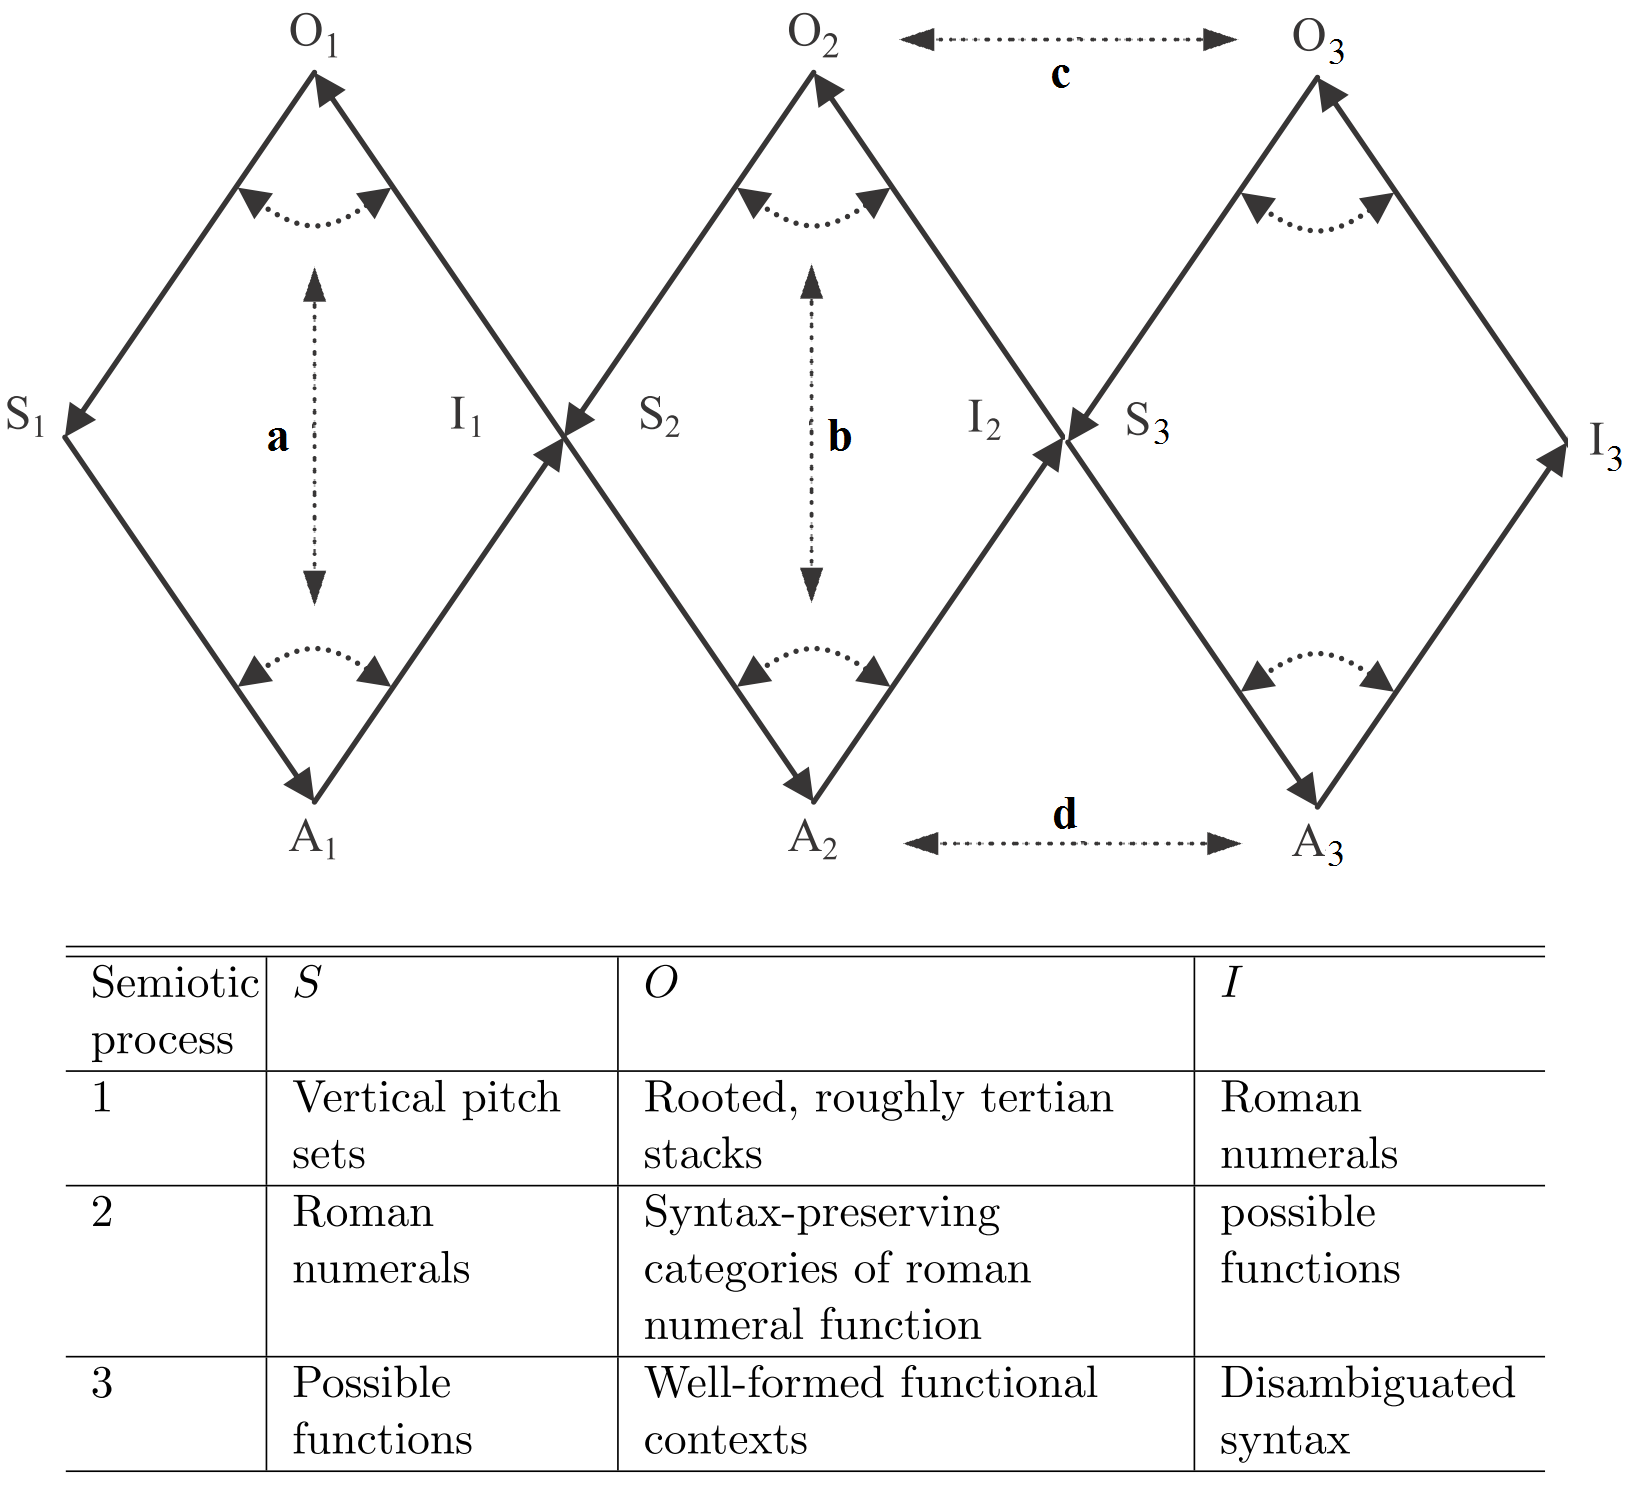
\includegraphics[width=6in]{kockelman_3simple.png}
\end{figure}

The dotted lines on Figure~\ref{k_t} denote the relations between relations underpinning (and undermining) semiotic communication.  First, as in the standard Kockelman framing, the properties and indices of the objects $O$ and the knowledge and actions of the agents $A$ make sense in complementary ways, as indicated by arrow (\textbf{a}).  The assignment of roman numerals $I_1$, for example, makes sense given the significant properties of $O_1$ only if the local pitch indices $S_1$ sign categories of key-rooted chords; the categories only have such indices by virtue of their selection by the agent.  Arrow (\textbf{b}) may describe a directly analogous process, where the identification of potential functions $I_2$ makes sense given the significant properties of $O_2$ -- that syntactic categories are indexed and signed by roman numerals.  Since the roman numeral label $I_1$ arose from content-driven analysis, with verticalities standing for their pitch-identified categories, $A_2$ may relate to $O_2$ in the same way (and with the same immediate ignorance of contextual or temporal information other than key).  The agents communicate across $S_1 \rightarrow I_2$ by virtue of this semiotic channel, where indices sign categories of verticalities.%TODO: check where Kockelman discusses channels?

From the right hand side of the diagram, channel comparison can be run in reverse.  $A_3$ cannot examine the potential functions $I_2 = S_3$ atemporally; without context, there is no way to determine whether or not a functional assignment will result in well-formed syntax.\footnote{Even in the limited string-matching case for well-formedness rules, where this might be done through examining a table of acceptable function strings, their \emph{ordering} must matter and will encode directly temporal properties into $O_3$.}  The properties of well-formed contexts explicitly require temporal progression indices, orderings of functions in time, to narrow down the potential assignments to one syntactic label $I_3$.  But if the $A_3 \rightarrow A_2$ relation (arrow (\textbf{d})) is mediated by the $O_3 \rightarrow  O_2$ relation (arrow (\textbf{c})), the different ontological conditions of the object categories necessitate strongly differentiated analytical interpreters.  Conversely, if the agents share goals, methods, or communicative channels, the resulting close relation $A_3 
\rightarrow A_2$ implies that the ontologically-(non)distinct categories $O_2$ and $O_3$ will inform one another.

I claim that syntax-preserving categories of roman numeral function $O_2$ are systematically over-determined, both for Terefenko and generally.  Verticalities end up in these categories by virtue of their atemporal pitch indices, but the well-formedness of the resulting parsings depends on strongly (perhaps exclusively) temporal indices.  To be pedantic but specific: two different voicings of ``the same" roman numeral get mapped to the same label by $A_1$ based on their \emph{contents}, and then that roman numeral's ultimate functional assignment $I_3$ relies on the heterogenous category's temporal progression \emph{contexts}.\footnote{I echo here terminology employed by \cite{white2013}.  See, for example, his gloss of Kopp on p.\ 183: ``Harmonic function, then, depends upon a chord's content and/or context, and functional categorizations can either emphasize the former or the latter."  Generally, I strongly sympathize with White's pursuit of a context-only syntax, though I doubt its possibility on semiotic grounds.}  When an analyst like Levine refers to a chord that is $V$-like, that particular sign could stand for objects in ontologies relevant to $O_1$, $O_2$, or $O_3$, or (more likely) some combination.

I will argue in what remains that contextual parsing is parasitic on content parsing in an explicitly semiotic sense defined by Kockelman.  Corpus analytical projects like this one can be framed to maximize the overlap between these sets of ontological constraints, but any algorithmic communication with human agents will introduce necessary misinterpretation.  I advocate a paradigm which embraces this misinterpretation as productive, limiting what we can know but hopefully broadening what we can do.

\section{Affordances and limits of a new (or many) paradigm(s)}
%temporality all the way down, pitch structure pushed out as much as possible
%affords claims of progression similarity at multiple time scale with as much confidence as possible
%still assumes all kinds of things --  especially that moments of time containing the same scale-degrees ought to behave in the same way.  This is the inescapable kernel of the parasitic process
%great for assembling the generic norms that human agents could later use for local parsing

Chapters 2-4 approach the production of chords and syntactic categories with a different framing from the accounts diagrammed above.  As I walk through the algorithmic steps involved in that pipeline, an overarching theme will emerge: rather than employing content-driven semiotic processes, I embed temporal considerations as far into the categories and data representations as possible.  This is done not to unearth some ultimate truth about this or any corpus, but rather to align the pipeline's production of interpretants with particular types of musicological pursuits -- ones focused on syntactic temporal progressions.  

\subsection{YJaMP's semiotic pipeline}
%A_1: MIDI parser
Figure~\ref{k_j} frames five semiotic processes spanning different algorithmic agents in communication with one another across similar channels and within related ontologies.  Agents 1 and 2, at the left edge of the figure, turn raw MIDI data into pitch-class set time windows and scale-degree sets, respectively, and they do so across related channels (\textbf{a}) and (\textbf{b}).  For $A_1$ to produce its pitch-class set interpretants, it must take the pitch and time indices $S_1$ as signs standing for chord objects defined in a very particular way and toward particular ends.  As is usually the case for algorithmic objects, these ``chords" resemble those a human analyst might define or discuss, but with crucial differences -- and the nature of those differences both renders the interpretants useful for other algorithmic agents and partially blocks our ability to map harmonic intuitions onto them.
%Jones syntax diagram
%NB: has extra dotted arrows, most likely.
\begin{landscape}
\begin{figure}
	\centering
	\caption{One framing of the semiotic pipeline connecting the YJaMP corpus to clusters of similar syntactic behavior.}%Possibly beef up?
	\label{k_j}
	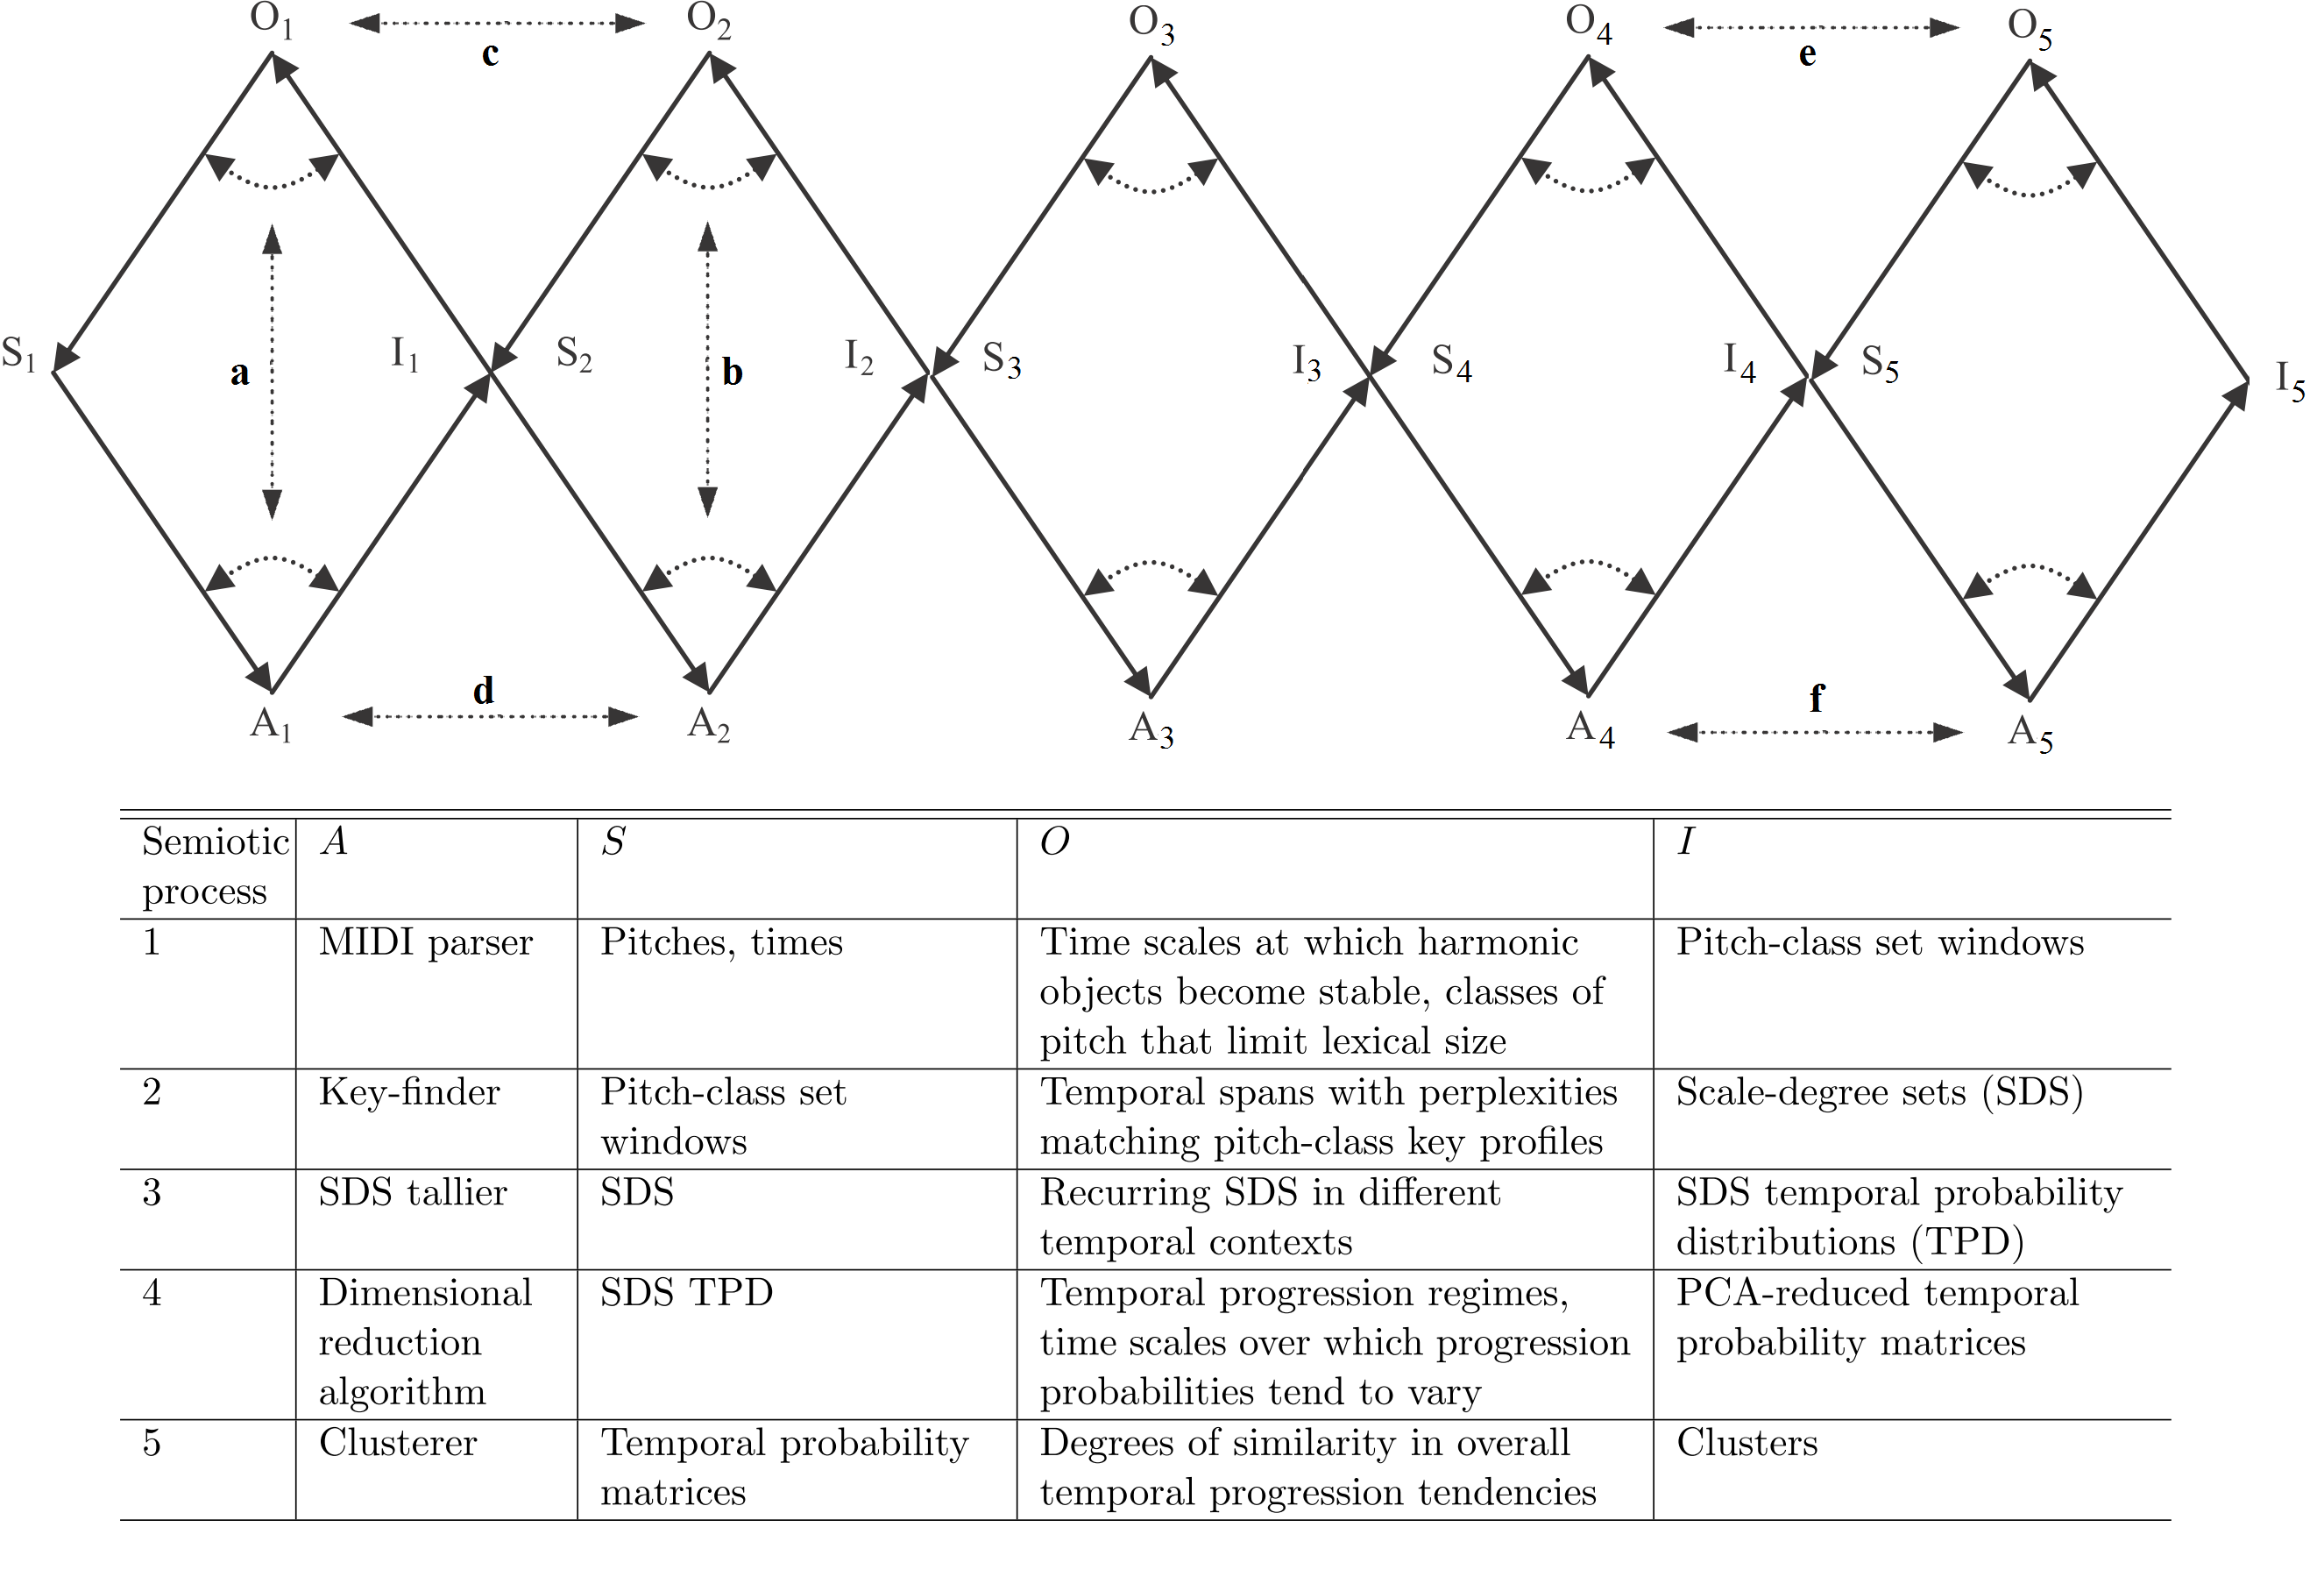
\includegraphics[width=8.25in]{kockelman_5jones.png}
\end{figure}
\end{landscape}


The objects $O_1$ occur at the smallest time scales where ``harmonies" -- roughly, collections with at least two or three pitches, as indicated by average window perplexity -- become stable, which tends to be around 50 milliseconds (see Chapter 2).  For $A_1$, time scales shorter than that sign some other kind of object or process, which a human might interpret as rolled chords with slightly different (but extremely close) onset times or very fast melodic runs.  $A_1$ does not know what these other objects are, of course, but it knows that the time scale at which it interprets objects $O_1$ is a special one -- special for the algorithm, in that it optimizes certain information-theoretic criteria, and special for us, in that it defines temporal objects well-suited to any theory purporting to treat chord progressions (e.g., the rest of the pipeline).

$A_1$ also assumes and generates objects with particular pitch properties.  For this agent, a voicing is not a chord; labeling each individual voicing type separately produces a very large and sparsely-populated vocabulary.  In order to select ``chords"  which may carry meaningful temporal progression statistics and recur across the corpus in many contexts (that is, to enable the task of the algorithmic agents with which it will communicate), $A_1$ turns pitch indices $S_1$ into pitch-class interpretants $I_1$.  This builds in a particular kind of ``bias," in Gjerdingen's sense (cf.\ Chapter 2), assuming that statements regarding harmonic progression might profit from this descriptive basis.  But \emph{any} analytical system involves labeling bias, and the relation between $A_1$ and the chord objects $O_1$ (given by dotted line (\textbf{a})) is chosen to align that bias with the specific conditions necessary for semiotic processes further down the pipeline.  If $A_2$ is coded and designed to use the interpretants produced by $A_1$ for a particular purpose (an inter-agent communicative relation indicated by arrow (\textbf{d})), then the properties ascribed to $O_1$ and $O_2$ ought to share modes of indexicality and significance (the (\textbf{c}) arrow).

%A_2: key-finder
After the MIDI parser ($A_1$) produces short-duration pitch-class set windows ($I_1$), the key-finder ($A_2$) interprets combinations of those windows as signs ($S_2$) indexing key spans ($O_2$).  As in relation (\textbf{a}), where the MIDI parser selects and interprets chord objects based on their distributional perplexity in time and a limited lexical size, the key-finder defines key spans as time windows with pitch-class perplexities similar to empirically-derived key profiles (Bellman-Budge, here, though other profiles have similar perplexities).  For $A_2$, spans governed by a particular key have no necessary chord structures, progressions, or cadential rhetoric -- they are defined by the relative proportion of scale degrees sounded during the span.\footnote{I note that assumptions regarding chord structure and progression may be read out of the key profiles, since scale degrees drawn from common roman-numeral chords receive high weightings, but the key-finder does not know this.}  Taken together, $A_1$ and $A_2$ trace a particular line of inquiry: if there is a time span at which harmonic objects first stabilize as quasi-verticalities, and if there is another time span at which the relative appearance of pitch-classes indexes or projects the distributional properties of key, then the scale-degree sets $I_2$ may be taken as consistently-defined labels for objects of harmonic interest.  $A_1$ and $A_2$ act as temporal filters, or as selecting ``sieves," in Kockelman's terms, each of which selects certain indices as significant toward the production of scale-degree set interpretants.

%A_3, sds-tallier
$A_3$, the scale-degree set tallier, has no direct access to the un-transposed MIDI data.  It examines the transposed scale-degree sets and time windows generated by the key-finder ($I_2 = S_3$), and it produces temporal probability distributions which make sense given progression objects (i.e., chords) specified by the ontology in which $O_3$ is embedded: each appearance of a particular scale-degree set indexes the general behavior of the scale-degree set across a token-type relation.  The tallier finds every token corresponding to a particular scale-degree set type (say, all performed instances of $[0,2,5,9]$) corpus-wide and records what other scale-degree set tokens appear within the subsequent five seconds (a span chosen based on the long-range predictivity of chords, which tapers off over time).  Each token has a particular temporal index (it is struck at exactly one time) and a specific sequence of other scale-degree set tokens which follow it.  The types, on the other hand, have a different ontological status: they do not occur at any particular time, and they are not associated with any specific sequence of chords.  Rather, the properties of each scale-degree set type consist of the probabilities with which many possible destination chords appear at given temporal delays.

This type-as-temporal-feature-bundle is a different kind of ``chord" object from $O_1$ or $O_2$, though its formation depends on them.  Crucially, the ontological difference between $O_2$ and $O_3$ is precisely the set of properties which permit generalizations regarding harmonic progressions.  When a jazz analyst claims that $V$ tends to go to $I$, he or she does not mean that a particular $V$ chord immediately proceeded to $I$ in one phrase of one performance.  The claim instead describes the frequent -- or most probable -- behavior of a type ``$V$" indexed by a wide variety of $V$ tokens.  The temporal probability distributions $I_3$ assigned to origin chord types $O_3$ encode that propositional relationship in explicit computational terms.  Unlike a human analyst, $I_3$ does \emph{not} say that a particular scale-degree set ``tends to go" anywhere, opting instead to provide a nuanced statistical portrait of what happens after each token appearance.  $I_3$ is not a judgment call; it is not a metaphysical claim; it makes no statement regarding what about a given scale-degree set might cause it to progress in any particular way; it does not even define exactly what a ``chord progression" might mean.  $I_3$ is a translation of facts communicated across and generated by the network of agents $A_1 \rightarrow A_2 \rightarrow A_3$.  It captures, in a minimal sense, the ontological shift necessary to move from statements regarding individual sonic moments $I_1$ or $I_2$ to generalizations about a chord type.  To my knowledge, every extant theory of harmonic syntax, function, or progression performs this ontological shift, but its nature is rarely specified -- indeed, for human-based analysis, it may be impossible to fully specify it.\footnote{Empirical or corpus analytical projects often perform this shift \emph{twice}, where individual tokens index types, and types generate or induce rules which then impact other tokens.  Human analysis which starts from categories constructed from notions of consonance or pitch content may only perform this shift \emph{once}, where the properties ascribed to a pre-defined category are inherited by tokens only during particular analysis.}  Here, the generalization receives statistical specification.

%A4: PCA reducer
If $A_3$ defines types from tokens, generalizing from many ``origin" chord instances to a far smaller number of indexed types, $A_4$ performs an analogous interpretation regarding chord-to-chord progressions in time.  For each origin chord scale-degree set, the dimensional reduction algorithm $A_4$ examines the probability distributions $I_3 = S_4$ which constitute the features ascribed to $O_3$.  How a chord (or rather chord \emph{type}) progresses is encoded in this data.  But statements regarding chord progression tendencies are not merely statistical portraits of nearby chords.  $A_4$ generalizes from the fine-grained temporal data to construct and define temporal progression regimes $O_4$ (cf.\ Chapter 3), ways of progressing in time.

%Human reduction
When a human analyst performs this reductive move, rhetoric, voice-leading, and phrase-level expectations inform distinctions between embellishing ``progressions," syntactic progressions, and chord-to-chord correlations deemed irrelevant to syntactic analysis.  Consider a temporally-ordered chord sequence $C_1, C_2, C_3,...,C_n$ for some large $n$.  Except under extraordinary circumstances, an analyst would rarely call the temporal correlation $C_1 \rightarrow C_{31}$ a ``progression."  But if $C_2$ and $C_3$ may be reduced away as voice exchanges or neighbor chords, the same analyst might well identify $C_1 \rightarrow C_4$ as a progression.  $A_4$ employs principal component analysis to produce similar types of ``progression" with a very different justification scheme.  Based on the temporal progression distributions, $A_4$ looks for combinations of time indices over which origin chord - destination chord combinations tend to show the highest variance in probability.  For most origin chords, a small number of components capture the lion's share of the variance in distributions, and the score given to each destination chord along each component indicates how well-captured its probabilistic variance is by that kind of temporal variance -- that mode of progression.\footnote{As indicated in Chapter 4, some caution is necessary here, as the (human) interpretation of a destination chord with high scores along more than one component is ripe for misinterpretation; does such a chord participate in more than one mode of ``progression," or do combinations of components themselves index modes of progression?}  $A_4$ may be thought to find chord progressions that a human would identify, but it really selects certain indices from the temporal probability distributions and assigns them as predicates for progression objects it constructs.

%A5: clusterer
Examining the temporal probability matrices in the dimensionally-reduced PCA basis ($I_4 = S_5$), the clustering algorithm ($A_5$) groups origin chords into categories of similar progression behavior $I_5$.  These clusters make sense in the presence of the temporal probability matrices $S_5$ only under the selection assumptions encoded in the clustering algorithm's optimization criteria and distance metric.  The properties of the chord cluster objects $O_5$ consist of the crude Manhattan distances between elements of each cluster.  Chords are ``similar" to one another if they are indexed by destination chords in statistically-similar ways across temporal progression regimes; since these properties depend on the indices selected by $A_4$, the relation between the dimensional reduction algorithm and the clusterer $A_4 \leftrightarrow A_5$ is mediated by the relation between the cluster objects and the temporal progression regimes $O_4 \leftrightarrow O_5$ (dotted arrows (\textbf{e}) and (\textbf{f}) on Figure~\ref{k_j}).

%incommensurability 
If one takes this semiotic chain as a black box $S_1 \rightarrow \blacksquare \rightarrow I_5$, where performances enter on one side and categories of chords come out the other, then the temptation to compare the black box to a brain and its outputs to human-generated categories of chord syntax is strong.\footnote{TODO: Think about whether and how much to unpack the computer science history of the black box, the Latourian implications of breaking it open like I do here.}  Indeed, the cognitive turn in corpus analytical music studies consists almost entirely of giving in to this temptation.  When David Temperley writes of a musical corpus that ``the model that makes the most accurate predictions about the data is then the most plausible model of the cognitive processes that gave rise to it," he assumes a fundamental similarity between algorithmic agents and processes in the human brain.\footnote{See \cite{temperley2010}, p.\ 355.  Temperley could get out of this by defining ``model" in an ends-oriented way, but the degree to which the ``homunculus talk" assigning human explanatory power to computational models is mitigated by that definition corresponds to the degree to which the ``model" could say nothing about cognitive processes.  (For a general critique of homunculus talk in cognitive research -- and a flurry of angry responses to that critique -- see \cite{mcginn2013}.)}  If a model clusters chords, for example, and produces results that mimic human-generated results, it may describe how humans make or perceive the music.  I intend the above framing to block this interpretation.  Not only do the algorithmic processes have no necessary neural correlates, but even the objects indicated -- the chords and categories and progressions selected, constructed, and interpreted by the algorithmic agents -- look like but \emph{are not} the objects of traditional (human) harmonic study.  That the clusters $I_5$ resemble traditional ideas regarding harmonic progression tendencies may be productive, useful, and applicable in a variety of circumstances (some of which I will elucidate below), but the semiotic referents upon which the algorithmic pipeline depends are fertile homophones, sounding like human statements but meaning something else.

\subsection{What do algorithmic agents know?  Or: Analysts as parasites.}
%All agents know stuff
As Wollheim notes of Loran, as Waters notes of Strunk, and as I note of Terefenko: what an analytical agent knows (or believes) informs the segmentation and classification processes on which that agent's activities and interpretants rely.  So what do the algorithmic agents of Figure~\ref{k_j} know?

$A_1$ knows the timescale at which collections of pitch classes tend to form, but not how they relate to one another; $A_2$ knows the timescale at which scale degrees tend to occur jointly in patterned ways, but not their ordering; $A_3$ knows the temporal ordering of token scale-degree sets, but not what general kinds and scales of ordering are important or common; $A_4$ knows that some particular temporal correlations underpin ordering patterns for any given origin chord, but not how origin chords relate to one another; $A_5$ knows how origin chord types relate to one another, but not any specific contexts.  Each agent acts as a sieve, filtering out indices to present as signed objects necessary for the next agent down the pipeline.

%the things we know are not fundamentally true
This prevents one kind of bias while enforcing another.  A certain form of hermeneutics is explicitly blocked, since particular expectations for chord type behavior cannot propagate backwards down the pipeline.  Where Loran's ostensibly-formal shape segmentation was informed by representational expectations further down the chain, no agent in the YJaMP pipeline has access to such information.  When $A_1$ segments a chord, it has no idea what the ultimate behavior of that chord might be or what any type it indexes could do.  But in each semiotic process given above, the kinds of properties the agent ascribes to each object have still been selected in a way suited to more than one task.  Put another way, many different ontologies might support the isolated selection processes of a given agent, and only some of those align with the processes employed by other agents.  There are many other ways to segment a musical surface into chords; $A_1$ chooses a particular way which provides exactly the indices necessary for $A_2$ (and so on).  I do not claim that this is the ``right" way -- emphatically the opposite.  I mean the above framing as a demonstration that there can be no ``right" way.

%parasitism
I embed temporal properties as far back into the pipeline as possible, but there is still no guarantee that the objects produced by the segmentation of $A_1$ and $A_2$ can produce or bear the kinds of properties required by agents $A_4$ and $A_5$.  Since each successive agent interprets the previous agent's interpretants in light of its own ontology, the signs necessarily afford (mis)direction toward other ends.  If this were not the case, $A_3$ could not produce temporal progression statistics from $A_2$'s scale-degree sets, since those sets all carried properties corresponding to distinct times and contexts.  Kockelman writes that if an object ``implies (embodies or indexes) other ends it might be directed to serve or indeed implies any way it may fail to serve an end (whether original or diverted)... [t]he parasite is whatever inhabits such implications."\footnote{\cite{kockelman2013}, p.\ 15.}  I claim that any context-oriented interpretant of a kind similar to that produced by $A_3$, $A_4$, or $A_5$ is parasitic on any content-oriented labeling systems similar to those produced by $A_1$ and $A_2$.  ``Just as a sign may (be taken to) stand for the wrong object," Kockelman reminds us, ``a  sign may also give rise to the wrong interpretant.  In this way, to return to our parasites, the \emph{tokens} instantiated may fail to conform to the \emph{types} selected."\footnote{\cite{kockelman2013}, p.\ 20.}  While membership in a given cluster, for example, is determined by type-level similarity in temporal progression statistics, membership in a given type $[0,2,5,9]$ is still assigned on the basis of the scale-degree content of a given token.  In the above pipeline, the contextual behavior of each token is embedded in the type's properties in a traceable way, but any resulting statements regarding the progression behavior of types is parasitic on chord tokens; content labels are misdirected to bear contextual properties.

%failure is inevitable
This is not a unique feature of the pipeline framed here.  In fact, this pipeline attempts to minimize the potential for parasitic misdirection, since the properties of literally every token are embedded in the properties of the scale-degree set types and clusters.  But once a probability distribution is calculated, information is lost about any given token.  The task of generalizing about harmonic progressions is inherently and unavoidably parasitic. So long as analysts (human or algorithmic) wish to produce interpretants identifying the temporal behavior of types indexed by pitch sets, pitch-class sets, scale-degree sets, or any other quasi-atemporal signs, the progressions we attribute to chord types will always misdirect token notation and permit failure.\footnote{If I want to sound really crazy, I could ask here if there can be such a thing as content-free labeling.  It seems like this might be possible with a radical re-orientation of harmonic inquiry, where each token is described purely in terms of its surroundings in some explicit way.  Would the results be tautological or impossible?}

\subsection{What can these interpretants do?}
%but failure is not always bad
This is not bad.  ``Failure," in a semiotic sense appropriate to the parasite, consists partly in cases where a token assigned to a type does not properly inherit or exhibit or index properties assigned to that type.  When in a particular phrase a chord does not behave as the chord's pitches might lead us to expect, analysis is not ruined.  By insisting (and demonstrating) that the many tokens with the same scale-degree content participate in a variety of progressions with statistically normative properties, we force open a door for hermeneutic interpretation and attentiveness to individuation.  A pipeline implicating no semiotic parasitism, it seems, would amount to a re-indexing of the input signs with no gains in generality.

A model which treats each individual token as its own type will not fail; an algorithm could reliably indicate which chord tokens succeed any temporally-specific token in the corpus at any time delay.  But such models do not reduce the complexity of the domain in any way, and some balance between failure and usefulness is required.  This balance (and the nature of the resulting semiotic failures and uses permitted) depends on the interpretive ends desired and pursued by the analyst at the end of the chain.  Several such analysts afforded by the pipeline of Chapters 2-4, both algorithmic and human, appear below.

%new-paradigm affordances designed to take parasitic advantage of the pipeline
\begin{enumerate}
	\item If an analyst seeks a high-level portrait of general temporal behavior at phonetic, syntactic, or long-range time scales, he or she might employ another algorithmic agent to tally the cluster-to-cluster transitions occurring at that time scale.  There are many ways this might be done, but perhaps the simplest is to modify the scale-degree set tallier $A_3$ to view cluster tags as input signs $S_3^{\prime}$ and produce temporal probability distributions $I_4^{\prime}$ for where tokens from those clusters tend to progress.  The same PCA reduction techniques would apply to these new distributions, re-encoding temporal progression regimes on the set of clusters, rather than the lexicon of scale-degree sets.
	
For example, if we want to know where chords in cluster 8 ($[0,2,5,7,9],[0,2,5,9],[2,5,9]$) tend to progress, we need to make several decisions: we might count or rule out progressions which remain within the cluster (like $[2,5,9] \rightarrow [0,2,5,9]$), we might choose different time scales, and we might index those time scales with millisecond windows or PCA-reduced basis components.  Table~\ref{8_progs} consists of interpretants produced under one set of those conditions.  Here, the tallier excludes intra-category transitions and looks for the shortest-scale progressions that result, as indexed by large PCA component 1 scores.
	
	\begin{table}
	\centering
	\caption{The top PCA component 1 (short time scale) destination chord clusters for origin chord cluster 8.  If cluster 8 contains $ii$-like chords, we might note that nearly all of the prominent destination chord clusters are $V$-like.}
	\label{8_progs}
	\begin{tabular}{p{0.75in} | p{0.75in} | >{\raggedright}p{1in} | >{\raggedright\arraybackslash}p{1in} }
	\hline\hline
	Destination cluster & PCA1 loading & Cluster example & Human interpretant\\ \hline
	45 & 7.74 & $[2,5,7,9,10]$ & $v^9$\\ \hline
	9 & 7.22 & $[0,4,5,9]$ & $IV^7$\\ \hline
	14 & 5.36 & $[2,5,7,11]$ & $V^7$\\ \hline
	13 & 4.96 & $[5,7,9,11]$ & $V^9$\\ \hline
	23 & 4.53 & $[2,5,9,10]$ & $\flat VII^{M7}$?\\ \hline
	48 & 4.47 & $[5,7,11]$ & $V^7$\\ \hline
	59 & 2.82 & $[7,8,11]$ & ?\\ \hline
	\end{tabular}
	\end{table}
	
The table lists the destination chord cluster labels (column one) with highest PCA-1 scores (column two) in descending order.  These columns are the tallier's actual interpretants, while the remaining two columns are my attempt to re-attach humans to the output.  Column three lists a single scale-degree set I have selected from the destination cluster (the full contents of which are listed on Table~\ref{memb}), and column four provides my rough gloss of what that chord might resemble in traditional theory parlance.  The algorithmic agents here do not know that several of these clusters resemble one another (like the $V^7$ and $V^9$ chords) -- only that tokens from these clusters frequently appear at similar, short time scales after a token from cluster 8.  My roman-numeral interpretations are explicitly parasitic on the algorithmic interpretants.  The pipeline's statistics do not prove that, say, ``$ii$ chords go to $V^7$ chords," but they provide a statistical language for specifying a meaning for such statements in a way accountable to the performance data.  And as with the mysterious appearance of $\flat VII^{M7}$ in Table~\ref{8_progs}, cluster type-level progression claims often produce statements counter-intuitive to a human analyst.  (Does this stand in for subtonic-type cadences in place of the more expected dominant $\flat VII^7$?)  Statements of this kind regarding cluster type progression properties might lead a human analyst down a variety of productive lines of inquiry.  These type-level properties cannot readily accomplish token-level phrase-parsing tasks of the kind performed by Terefenko, Strunk, or Waters, but they may inform or generate the norms on which those parsings rely.
	
	\item  The pipeline's direct connection to certain performance indices affords the isolation of seemingly non-normative token behavior.  When tallying the progression behavior of $[2,7,11]$ as a type, two strange claims emerge from the pipeline: that $[2,7,11]$ belongs in cluster 12, which contains many unambiguous tonic scale-degree sets (cf.\ Table~\ref{memb}), and that it progresses on many occasions directly to $[0,5,9]$.  Were these seventh chords, blues progressions might readily contain them, but their triadic nature appears unstylistic when compared to similar statements made under traditional harmonic analysis paradigms.

Recalling that the type is parasitic on the token, we may employ a new algorithmic agent to search for specific times where this progression takes place in the corpus.  In this case, doing so allows us to identify that 80\% of the token occurrences of $[2,7,11] \rightarrow [0,5,9]$ appear in just two recorded tunes: Alex Dubovoy's performance of ``Stella by Starlight," and Joe McWilliams's performance of ``If I had You."  Both performances feature prominent intro and outro ``riffs," vamp-like progressions setting the stage for the sound-world of the tune.\footnote{TODO: Who writes about riffs and vamps?}  The $[2,7,11] \rightarrow [0,5,9]$ progressions appear almost exclusively in these intros/outros.  This might imply that different syntactic constraints operate in vamp-like, repetitive harmonic contexts, and that intros and outros lying outside the purview of a tune's head and chord progression might afford different kinds of progression from the rest of the tune.\footnote{TODO: Surely somebody writes about this.}  The progression is a ``special effect" of sorts, and the pipeline's failure to re-produce traditional expectation allows us to unearth this particular behavior.

It might also imply that vamp-like progressions defy the usefulness of the key-finding algorithm.  Figure~\ref{alex_outro} provides a MIDI readout in ``piano roll" format (keyboard pitch versus time) for Dubovoy's ``Stella" outro, which consists primarily of three major triads transposed in parallel -- $BM \rightarrow AM \rightarrow A\flat M$.  Here we see that the key-finding algorithm has interpreted $BM \rightarrow AM$ as $[2,7,11] \rightarrow [0,5,9]$ merely in an attempt to fit an unusual progression into a ``key."  The repeated vamp produces a very consistent pitch-class distribution over a span of tens of seconds which loosely matches a traditional key profile.  The strong presence of $\{B,D\sharp,F\sharp\}$, $\{A,C\sharp,E\}$, and $\{A\flat,C,E\flat\}=\{G\sharp,B\sharp,D\sharp\}$ produces roughly the key-weightings of the $EM$ profile, despite its rhetorical and cadential implausibility.  After Dubovoy finishes the last rotation of the head in $B\flat M$, he sidesteps the concluding tonic chord, replacing it with $BM$ and initiating the vamp.  Since the resulting progression does not resemble the $B\flat M$ material which preceded it, the keyfinder makes its best guess.  Note that the keyfinder \emph{is not wrong}, semiotically: the properties the algorithm applied to a ``key" are different from the properties a human might consider important.  Key assignment thus does not directly mimic human activity, but it still serves to isolate progressions for aggregate statistics -- the keyfinder assigns McWilliams's vamp a similarly-``wrong" key, which nevertheless allows the tallier to see a similarity in the two progressions.
	\begin{landscape}
	\begin{figure}
		\centering
		\caption{The final 25 seconds of Alex Dubovoy's performance of ``Stella by Starlight."  The vertical axis plots keyboard pitch, from low to high; the horizontal axis tracks time from left to right.  The red boxes indicate the consecutive major triads separated by a whole step that the scale-degree set producing keyfinder identifies as $[2,7,11]$ and $[0,5,9]$.}
		\label{alex_outro}
		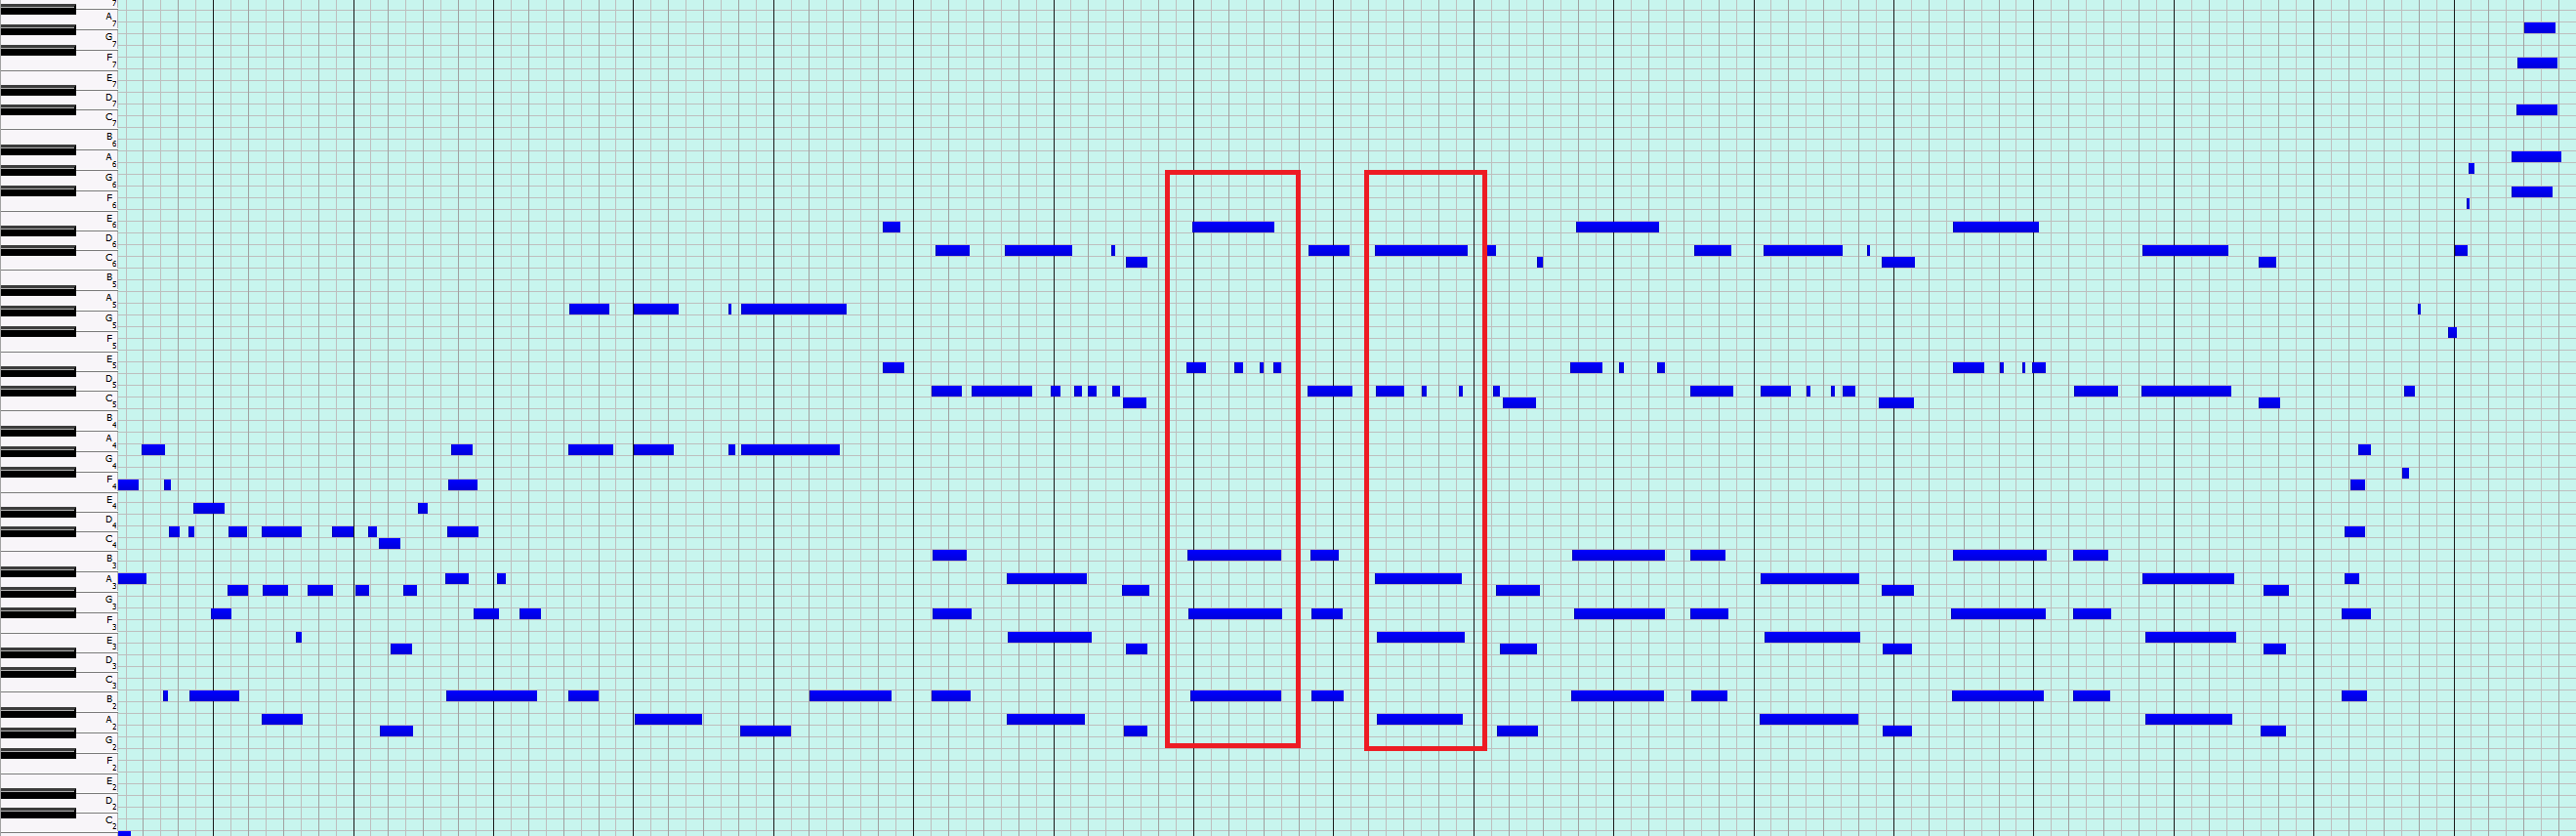
\includegraphics[width=8.75in]{alex_outro.png}
	\end{figure}
	\end{landscape}

Compared to a human analyst, the pipeline failed, both semiotically and practically -- this key parsing does not reflect human intuitions in a useful way.  But it (when combined with a human analyst) succeeded in locating a spot where normative key behavior is defied in an organized and systematic way.  To reproduce this mode of inquiry, a human analyst might compare his or her syntactic intuitions to progression-statistical interpretants produced by algorithmic agents and run the pipeline backwards, so to speak, to identify patterns captured by the type properties but about which we have no \emph{a priori} intuitions.  As I have argued elsewhere, corpus-analytical methods construct homogeneous harmonic norms while also providing a means for identifying and extracting their heterogeneous remainders.\footnote{I refer here to unpublished work I presented at the New England Conference of Music Theorists in 2015.  \cite{jones2015}.}  Humans and algorithms disagree regarding what a key is, but this disagreement allows the YJaMP pipeline to sign patterned progressions outside frame reachable by other paradigms.

%Well-formedness rules, CCG grammars	
	\item Generally speaking, the behavior modeled by the cluster memberships and type progression probability distributions will prove more useful in aggregating normative corpus-wide trends than producing local parsings.  Linguistically-inclined analysts will note that the former kind of data guides the production of well-formedness rules like those employed at the end of the semiotic chain I attributed to Terefenko in Figure~\ref{k_t}.  To disambiguate potential parsings, Terefenko judges the possible functional category assignments ($I_2 = S_3$ on Figure~\ref{k_t}) by the degree to which they produce syntactically well-formed contextual phrases.  As my framing implies, such judgments rely on the properties of well-formed phrases or well-formedness rules ($O_3$).  Type-level cluster transition statistics provide one possible grounding for such rules drawn from a given corpus.
	
Sophisticated natural language processing (NLP) approaches to jazz analysis typically encode well-formedness rules into a grammatical model and assess their appropriateness based on how well they reproduce ``gold standard" analyses (usually produced by a human and from lead sheets).  \cite{granroth2012}, for example, extends and employs earlier Combinatory Categorial Grammar (CCG) approaches to constrain lexical combinations based on the behavior of the categories to which they belong.  But as inputs for their grammatical parsings, the authors ``have hand-crafted a lexicon containing categories suitable for assigning harmonic interpretations to chords," and the resulting categories depend very strongly on their assumption that identifiable roots and chord qualities form the basis of syntactic categories.\footnote{\cite{granroth2012}, p.\ 4.}  The pipeline of chapters 2-4 provides an alternate method for generating such a lexicon, and CCG or other grammatical methods might be employed to turn cluster assignments as signs into well-formed parsings as interpretants.

I leave open the question of what type of well-formedness rules would best capture the temporal progression behavior of YJaMP or any other jazz corpus, though (as Chapter 1 implies) I am skeptical of the deeply recursive hierarchical and semantic structure Granroth-Wilding and Steedman employ.  But the use of probabilistic grammars based on data-driven lexical categories and the production of temporal progression norms could allow an analyst to produce local parsing interpretants from the otherwise ill-suited type-level statistics given here.  Crucially, the lexical assignments offered here do not encode any pre-conceptions regarding harmonic norms other than that they involve locally-transposed near-verticalities and their relative deployments over time.%TODO: should I beef up my critique of what the goal of such modeling methods is?  Maybe I should check what part of that ought to go in chapter 1.  

%Algorithmic composition
	\item A set of well-formedness rules based on the norms of a corpus can do more than guide parsing choices.  From the earliest research on computational grammars in music studies, parsers have appeared alongside \emph{producers} of music, generative routines which leverage rules drawn from a corpus or encoded based on human intuitions in order to support algorithmic composition efforts.\footnote{See \cite{fernandez2013}.}  The specific indices captured by the statistics drawn from YJaMP are well suited to such a task, as they already encode computational generalizations regarding temporal ordering at many time scales.  As a recent undergraduate computer science thesis at Yale demonstrated, comparatively simple stochastic grammars can take the temporal probability distributions producced here and use them to generate weighted distributions from which chords may be drawn at random.\footnote{See \cite{zitomer2016}.}  The results do not produce jazz in a way that humans do, but they provide two distinct benefits: they open algorithmic composition to a much wider lexicon of chords than roman numeral or lead sheet chord symbol-based methods, providing a fertile extension to the lexical constraints of algorithmic composers like Kulitta.\footnote{For details on Kulitta, see \cite{quick2014}.} And they encode temporal correlations at many time scales, allowing the development of sophisticated probabilistic models.

%Common to both grammatical parsings based on well-formedness rules and probabilistic composition approaches: Bayesian updating, especially in the context of Markov-type models.  This pipeline uniquely well-suited to temporally-sensitive Markov approaches, like the mixed-order models of Saul \& Pereira
	\item In general, both generating algorithmic compositions and constructing well-formedness rules applicable to individual phrase parsings involve choices regarding how to align permitted elements of the harmonic lexicon into syntactic temporal orderings.  The semiotic agents and interpretants of the YJaMP pipeline are uniquely well-suited to Markovian probabilistic models designed to produce and assess the likelihood of such orderings.  As with many corpus analytical approaches in music theory, consideration of this class of models involves engagement with research in computational linguistics.  In what remains, I will briefly frame a Markovian extension to the YJaMP pipeline suggestive for future work.
	
%explain classical n-gram Markov model, and shoot it down on temporal grounds
%footnote some n-gram models in music; bigrams and trigrams are good (like White?), but moving back farther than that is hard
Traditional $n$-gram modeling focuses on the moment at which a new or next chord's appearance in a sentence (linguistics) or progression (harmony) must be assessed probabilistically.  From a corpus of observation sequences, an $n$-gram model tallies all the ordered instances of $n$ consecutive tokens and produces probability distributions capturing what word (linguistics) or chord (harmony) tends to appear after every given combination of $n$ lexical elements.  Then, when the parser or generator encounters a sequence of elements $[C_1,C_2,C_3,...C_n]$ after which a new word or chord $C_{n+1}$ must be predicted, it draws on the knowledge encoded in the probability distributions -- after each sequence of $n$ elements, syntactically-structured corpora tend to display predictable patterns for the appearance of the $n+1$th element.\footnote{For a broader overview of $n$-gram methods, one can turn almost anywhere, these days -- but for a lucid and thorough place to start, see \cite{jurafsky2000}.}

The choice of how much of a history to give each such moment hinges on the choice of $n$.  Considering a larger number of previous chords yields more finely-grained predictions, but the increased subtlety comes at the cost of extreme sparsity: for a lexicon of size $L$, a given $n$-gram distribution will need probability estimates for $L^n$ possible orderings.  Many of these orderings may never occur in the training set, and various ``smoothing" measures attempt to account for such events by re-allocating them low but non-zero probability.  Alternately, when $n$-gram models encounter a previously-unseen combination of $n$ elements, they may ``back off" to smaller orders $n-j$ in a variety of ways.  With such smoothing and backoff adjustments, $n$-gram models have proven highly adept at predicting word and chord sequences, despite their radical dependence on only the most local, ordered context.

White and Quinn, Rohrmeier and Cross, and Raphael and Stoddard, \emph{inter alia}, have implemented bigram and trigram models of harmonic progression ($n=\{2,3\}$) with demonstrable success from corpora represented as sequences of roman numerals or scale degree sets.\footnote{\cite{white2013}; \cite{wq2017}; \cite{rohrmeier2008}; \cite{raphael2004}.}  Rohrmeier and Cross's methods, in particular, stand as a relatively close analog to the YJaMP pipeline in this context, as they employ agglomerative clustering based on bigram transition statistics.  Their model, like other common $n$-gram implementations in music theory, avoids the large-$n$ sparsity problem by tallying only quarter note sampling and immediate chord adjacencies.\footnote{See the segmentation discussion in part D of \cite{rohrmeier2008}.}

%transition to mixed-order Markov models
Like an $n$-gram model, the YJaMP temporal probability distributions inform the selection or likelihood of a new or next chord from the perspective of many temporally-previous chords.  But unlike common musical $n$-gram applications, a generative algorithm employing temporal data drawn from this pipeline may combine probabilistic contributions from each of the preceding chords individually at the time delay in question. Such an implementation would follow and extend the \emph{mixed-order} Markov model advocated in the linguistic context by Saul and Pereira.\footnote{See \cite{saul1997}.}

%summarize Saul \& Pereira
Mixed-order Markov models, sometimes called ``skip-$k$" models, treat non-adjacent predictive correlations.  If considering $n>2$ consecutive words yields a sparse distribution, a standard back-off procedure might consider some smaller $n$. But the one or two closest words to a given token may be relatively uninformative for structured contexts with long-range dependencies.  Mixed-order models allow probability contributions from further back in the chain at placement delays; if the $n=3$ distribution for a given lexicon is sparse, for example, a mixed-order model might nevertheless make its prediction by considering only the word preceding the moment of prediction by three (or $k$) words (hence: skip-$k$).  As Saul and Pereira note, mixed-order Markov models incorporate more temporal information while retaining limits on the size of the distribution's lexicon, decreasing model perplexity without an explosion of sparsely-populated $n$-gram states.\footnote{See \cite{saul1997}, \S 3.}

%Indicate analogous YJaMP pipeline interpretants
An algorithmic composer or parsing model could make analogous use of interpretants produced by the semiotic agents of the YJaMP pipeline.  For a given sequence of $n$ chords $[C_1,C_2,C_3,...C_n]$, an algorithm could assess the impact of each chord on the probable appearance of the $n+1$th chord with temporal probability distributions.  Since each $C_j$ for $1\leq j \leq n$ will fall at some temporal delay from $C_{n+1}$, its probabilistic contribution to the distribution from which $C_{n+1}$ will be drawn can arise from its distribution at time window $t= n+1-j$; this is precisely what is signed by the intepretants $I_3$ from Figure~\ref{k_j}.  Moreover, since each high-probability YJaMP origin chord can be associated with a PCA basis for its temporal progressions (by the dimensional reduction algorithmic agent $A_4$), a mixed-order algorithm could also take into account the time scales at which each particular $C_j$ tends to be most predictive, measured by PCA variance or distributional perplexity at $t=n+1-j$.  Chords with flat probability distributions at such times (like stable tonic chords at long $t$) could contribute less to the prediction of $C_{n+1}$ than chords with strong temporal correlations (like dominant-type chords at short $t$).  The very fact that the YJaMP pipeline generates chord types with detailed temporal properties that are difficult for a human to interpret renders its interpretants well-suited to such modeling.
\end{enumerate}

%sign off
%also nod to the fuzzy category assignment of aggregate Markov models, possibly name-drop factored language models? 
Each combination of agents above will draw on different indices and produce different interpretants, and each resulting pipeline must ensure that communicative ``failures" and parasitic re-interpretations push the research forward rather than hold it back.  If the preceding chapters offer anything of lasting use to a community of communicating agents with widely varied goals, I hope that its data representational paradigm imbricates temporality and semiotics in the production of harmonic syntax claims in a way which is flexible, generalizable, and aware of its limits.%general (Wollheimian) critique of formalism, description of how my methods escape the critique, affordances and possibilities for syntactic theories like mine
%\printindex
\bibliography{Diss_bib}
\bibliographystyle{plain}
\end{document}